\part{Unsourced Random Access \newline as Compressed Sensing}
\frame{\partpage}

% % % % % % % % % % % % % % % % % % % %

\begin{frame} \frametitle{Unsourced Random Access}
% % % % %
\hfill
\scalebox{0.5}{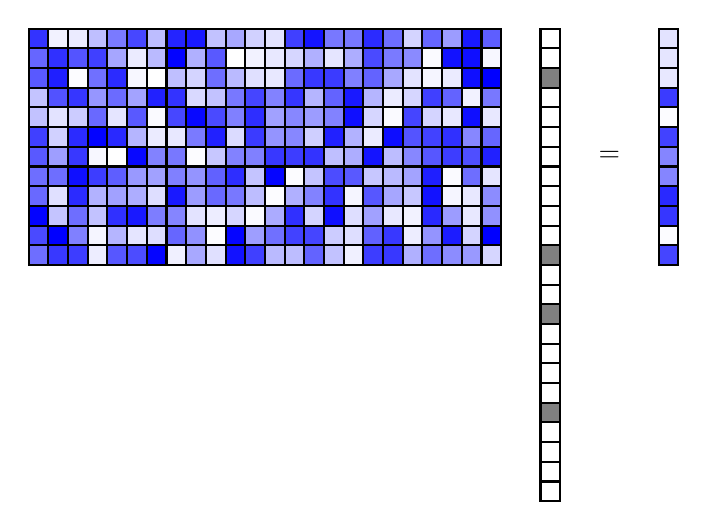
\begin{tikzpicture}
[draw=black, line width=0.75pt,
entry/.style={rectangle, draw, inner sep=0pt, minimum size=2.5mm},
symbol/.style={rectangle, draw, inner sep=0pt, minimum size=2.5mm}]

\node[entry, fill=blue!57] (x0y0) at (0.0,0.0) {};
\node[entry, fill=blue!71] (x0y1) at (0.0,0.25) {};
\node[entry, fill=blue!99] (x0y2) at (0.0,0.5) {};
\node[entry, fill=blue!59] (x0y3) at (0.0,0.75) {};
\node[entry, fill=blue!57] (x0y4) at (0.0,1.0) {};
\node[entry, fill=blue!65] (x0y5) at (0.0,1.25) {};
\node[entry, fill=blue!75] (x0y6) at (0.0,1.5) {};
\node[entry, fill=blue!24] (x0y7) at (0.0,1.75) {};
\node[entry, fill=blue!23] (x0y8) at (0.0,2.0) {};
\node[entry, fill=blue!65] (x0y9) at (0.0,2.25) {};
\node[entry, fill=blue!60] (x0y10) at (0.0,2.5) {};
\node[entry, fill=blue!80] (x0y11) at (0.0,2.75) {};

\node[entry, fill=blue!78] (x1y0) at (0.25,0.0) {};
\node[entry, fill=blue!101] (x1y1) at (0.25,0.25) {};
\node[entry, fill=blue!23] (x1y2) at (0.25,0.5) {};
\node[entry, fill=blue!12] (x1y3) at (0.25,0.75) {};
\node[entry, fill=blue!57] (x1y4) at (0.25,1.0) {};
\node[entry, fill=blue!38] (x1y5) at (0.25,1.25) {};
\node[entry, fill=blue!18] (x1y6) at (0.25,1.5) {};
\node[entry, fill=blue!11] (x1y7) at (0.25,1.75) {};
\node[entry, fill=blue!68] (x1y8) at (0.25,2.0) {};
\node[entry, fill=blue!88] (x1y9) at (0.25,2.25) {};
\node[entry, fill=blue!81] (x1y10) at (0.25,2.5) {};
\node[entry, fill=blue!5] (x1y11) at (0.25,2.75) {};

\node[entry, fill=blue!76] (x2y0) at (0.5,0.0) {};
\node[entry, fill=blue!50] (x2y1) at (0.5,0.25) {};
\node[entry, fill=blue!57] (x2y2) at (0.5,0.5) {};
\node[entry, fill=blue!83] (x2y3) at (0.5,0.75) {};
\node[entry, fill=blue!94] (x2y4) at (0.5,1.0) {};
\node[entry, fill=blue!78] (x2y5) at (0.5,1.25) {};
\node[entry, fill=blue!83] (x2y6) at (0.5,1.5) {};
\node[entry, fill=blue!20] (x2y7) at (0.5,1.75) {};
\node[entry, fill=blue!79] (x2y8) at (0.5,2.0) {};
\node[entry, fill=blue!1] (x2y9) at (0.5,2.25) {};
\node[entry, fill=blue!67] (x2y10) at (0.5,2.5) {};
\node[entry, fill=blue!8] (x2y11) at (0.5,2.75) {};

\node[entry, fill=blue!7] (x3y0) at (0.75,0.0) {};
\node[entry, fill=blue!4] (x3y1) at (0.75,0.25) {};
\node[entry, fill=blue!24] (x3y2) at (0.75,0.5) {};
\node[entry, fill=blue!30] (x3y3) at (0.75,0.75) {};
\node[entry, fill=blue!76] (x3y4) at (0.75,1.0) {};
\node[entry, fill=blue!3] (x3y5) at (0.75,1.25) {};
\node[entry, fill=blue!99] (x3y6) at (0.75,1.5) {};
\node[entry, fill=blue!59] (x3y7) at (0.75,1.75) {};
\node[entry, fill=blue!41] (x3y8) at (0.75,2.0) {};
\node[entry, fill=blue!56] (x3y9) at (0.75,2.25) {};
\node[entry, fill=blue!75] (x3y10) at (0.75,2.5) {};
\node[entry, fill=blue!25] (x3y11) at (0.75,2.75) {};

\node[entry, fill=blue!66] (x4y0) at (1.0,0.0) {};
\node[entry, fill=blue!29] (x4y1) at (1.0,0.25) {};
\node[entry, fill=blue!81] (x4y2) at (1.0,0.5) {};
\node[entry, fill=blue!37] (x4y3) at (1.0,0.75) {};
\node[entry, fill=blue!63] (x4y4) at (1.0,1.0) {};
\node[entry, fill=blue!0] (x4y5) at (1.0,1.25) {};
\node[entry, fill=blue!84] (x4y6) at (1.0,1.5) {};
\node[entry, fill=blue!10] (x4y7) at (1.0,1.75) {};
\node[entry, fill=blue!58] (x4y8) at (1.0,2.0) {};
\node[entry, fill=blue!83] (x4y9) at (1.0,2.25) {};
\node[entry, fill=blue!35] (x4y10) at (1.0,2.5) {};
\node[entry, fill=blue!52] (x4y11) at (1.0,2.75) {};

\node[entry, fill=blue!70] (x5y0) at (1.25,0.0) {};
\node[entry, fill=blue!10] (x5y1) at (1.25,0.25) {};
\node[entry, fill=blue!90] (x5y2) at (1.25,0.5) {};
\node[entry, fill=blue!32] (x5y3) at (1.25,0.75) {};
\node[entry, fill=blue!40] (x5y4) at (1.25,1.0) {};
\node[entry, fill=blue!97] (x5y5) at (1.25,1.25) {};
\node[entry, fill=blue!29] (x5y6) at (1.25,1.5) {};
\node[entry, fill=blue!65] (x5y7) at (1.25,1.75) {};
\node[entry, fill=blue!36] (x5y8) at (1.25,2.0) {};
\node[entry, fill=blue!3] (x5y9) at (1.25,2.25) {};
\node[entry, fill=blue!8] (x5y10) at (1.25,2.5) {};
\node[entry, fill=blue!72] (x5y11) at (1.25,2.75) {};

\node[entry, fill=blue!98] (x6y0) at (1.5,0.0) {};
\node[entry, fill=blue!13] (x6y1) at (1.5,0.25) {};
\node[entry, fill=blue!51] (x6y2) at (1.5,0.5) {};
\node[entry, fill=blue!13] (x6y3) at (1.5,0.75) {};
\node[entry, fill=blue!37] (x6y4) at (1.5,1.0) {};
\node[entry, fill=blue!49] (x6y5) at (1.5,1.25) {};
\node[entry, fill=blue!8] (x6y6) at (1.5,1.5) {};
\node[entry, fill=blue!2] (x6y7) at (1.5,1.75) {};
\node[entry, fill=blue!87] (x6y8) at (1.5,2.0) {};
\node[entry, fill=blue!0] (x6y9) at (1.5,2.25) {};
\node[entry, fill=blue!27] (x6y10) at (1.5,2.5) {};
\node[entry, fill=blue!26] (x6y11) at (1.5,2.75) {};

\node[entry, fill=blue!6] (x7y0) at (1.75,0.0) {};
\node[entry, fill=blue!60] (x7y1) at (1.75,0.25) {};
\node[entry, fill=blue!48] (x7y2) at (1.75,0.5) {};
\node[entry, fill=blue!90] (x7y3) at (1.75,0.75) {};
\node[entry, fill=blue!50] (x7y4) at (1.75,1.0) {};
\node[entry, fill=blue!53] (x7y5) at (1.75,1.25) {};
\node[entry, fill=blue!9] (x7y6) at (1.75,1.5) {};
\node[entry, fill=blue!72] (x7y7) at (1.75,1.75) {};
\node[entry, fill=blue!80] (x7y8) at (1.75,2.0) {};
\node[entry, fill=blue!25] (x7y9) at (1.75,2.25) {};
\node[entry, fill=blue!99] (x7y10) at (1.75,2.5) {};
\node[entry, fill=blue!86] (x7y11) at (1.75,2.75) {};

\node[entry, fill=blue!34] (x8y0) at (2.0,0.0) {};
\node[entry, fill=blue!43] (x8y1) at (2.0,0.25) {};
\node[entry, fill=blue!11] (x8y2) at (2.0,0.5) {};
\node[entry, fill=blue!39] (x8y3) at (2.0,0.75) {};
\node[entry, fill=blue!42] (x8y4) at (2.0,1.0) {};
\node[entry, fill=blue!1] (x8y5) at (2.0,1.25) {};
\node[entry, fill=blue!52] (x8y6) at (2.0,1.5) {};
\node[entry, fill=blue!97] (x8y7) at (2.0,1.75) {};
\node[entry, fill=blue!15] (x8y8) at (2.0,2.0) {};
\node[entry, fill=blue!17] (x8y9) at (2.0,2.25) {};
\node[entry, fill=blue!31] (x8y10) at (2.0,2.5) {};
\node[entry, fill=blue!90] (x8y11) at (2.0,2.75) {};

\node[entry, fill=blue!12] (x9y0) at (2.25,0.0) {};
\node[entry, fill=blue!1] (x9y1) at (2.25,0.25) {};
\node[entry, fill=blue!7] (x9y2) at (2.25,0.5) {};
\node[entry, fill=blue!59] (x9y3) at (2.25,0.75) {};
\node[entry, fill=blue!62] (x9y4) at (2.25,1.0) {};
\node[entry, fill=blue!22] (x9y5) at (2.25,1.25) {};
\node[entry, fill=blue!87] (x9y6) at (2.25,1.5) {};
\node[entry, fill=blue!71] (x9y7) at (2.25,1.75) {};
\node[entry, fill=blue!24] (x9y8) at (2.25,2.0) {};
\node[entry, fill=blue!57] (x9y9) at (2.25,2.25) {};
\node[entry, fill=blue!65] (x9y10) at (2.25,2.5) {};
\node[entry, fill=blue!24] (x9y11) at (2.25,2.75) {};

\node[entry, fill=blue!93] (x10y0) at (2.5,0.0) {};
\node[entry, fill=blue!98] (x10y1) at (2.5,0.25) {};
\node[entry, fill=blue!16] (x10y2) at (2.5,0.5) {};
\node[entry, fill=blue!53] (x10y3) at (2.5,0.75) {};
\node[entry, fill=blue!82] (x10y4) at (2.5,1.0) {};
\node[entry, fill=blue!49] (x10y5) at (2.5,1.25) {};
\node[entry, fill=blue!14] (x10y6) at (2.5,1.5) {};
\node[entry, fill=blue!50] (x10y7) at (2.5,1.75) {};
\node[entry, fill=blue!53] (x10y8) at (2.5,2.0) {};
\node[entry, fill=blue!27] (x10y9) at (2.5,2.25) {};
\node[entry, fill=blue!0] (x10y10) at (2.5,2.5) {};
\node[entry, fill=blue!34] (x10y11) at (2.5,2.75) {};

\node[entry, fill=blue!75] (x11y0) at (2.75,0.0) {};
\node[entry, fill=blue!38] (x11y1) at (2.75,0.25) {};
\node[entry, fill=blue!2] (x11y2) at (2.75,0.5) {};
\node[entry, fill=blue!26] (x11y3) at (2.75,0.75) {};
\node[entry, fill=blue!23] (x11y4) at (2.75,1.0) {};
\node[entry, fill=blue!50] (x11y5) at (2.75,1.25) {};
\node[entry, fill=blue!77] (x11y6) at (2.75,1.5) {};
\node[entry, fill=blue!82] (x11y7) at (2.75,1.75) {};
\node[entry, fill=blue!73] (x11y8) at (2.75,2.0) {};
\node[entry, fill=blue!12] (x11y9) at (2.75,2.25) {};
\node[entry, fill=blue!5] (x11y10) at (2.75,2.5) {};
\node[entry, fill=blue!18] (x11y11) at (2.75,2.75) {};

\node[entry, fill=blue!27] (x12y0) at (3.0,0.0) {};
\node[entry, fill=blue!56] (x12y1) at (3.0,0.25) {};
\node[entry, fill=blue!33] (x12y2) at (3.0,0.5) {};
\node[entry, fill=blue!1] (x12y3) at (3.0,0.75) {};
\node[entry, fill=blue!98] (x12y4) at (3.0,1.0) {};
\node[entry, fill=blue!78] (x12y5) at (3.0,1.25) {};
\node[entry, fill=blue!42] (x12y6) at (3.0,1.5) {};
\node[entry, fill=blue!37] (x12y7) at (3.0,1.75) {};
\node[entry, fill=blue!49] (x12y8) at (3.0,2.0) {};
\node[entry, fill=blue!9] (x12y9) at (3.0,2.25) {};
\node[entry, fill=blue!9] (x12y10) at (3.0,2.5) {};
\node[entry, fill=blue!11] (x12y11) at (3.0,2.75) {};

\node[entry, fill=blue!26] (x13y0) at (3.25,0.0) {};
\node[entry, fill=blue!74] (x13y1) at (3.25,0.25) {};
\node[entry, fill=blue!81] (x13y2) at (3.25,0.5) {};
\node[entry, fill=blue!31] (x13y3) at (3.25,0.75) {};
\node[entry, fill=blue!1] (x13y4) at (3.25,1.0) {};
\node[entry, fill=blue!76] (x13y5) at (3.25,1.25) {};
\node[entry, fill=blue!47] (x13y6) at (3.25,1.5) {};
\node[entry, fill=blue!47] (x13y7) at (3.25,1.75) {};
\node[entry, fill=blue!79] (x13y8) at (3.25,2.0) {};
\node[entry, fill=blue!58] (x13y9) at (3.25,2.25) {};
\node[entry, fill=blue!16] (x13y10) at (3.25,2.5) {};
\node[entry, fill=blue!75] (x13y11) at (3.25,2.75) {};

\node[entry, fill=blue!61] (x14y0) at (3.5,0.0) {};
\node[entry, fill=blue!73] (x14y1) at (3.5,0.25) {};
\node[entry, fill=blue!17] (x14y2) at (3.5,0.5) {};
\node[entry, fill=blue!49] (x14y3) at (3.5,0.75) {};
\node[entry, fill=blue!23] (x14y4) at (3.5,1.0) {};
\node[entry, fill=blue!80] (x14y5) at (3.5,1.25) {};
\node[entry, fill=blue!19] (x14y6) at (3.5,1.5) {};
\node[entry, fill=blue!39] (x14y7) at (3.5,1.75) {};
\node[entry, fill=blue!29] (x14y8) at (3.5,2.0) {};
\node[entry, fill=blue!78] (x14y9) at (3.5,2.25) {};
\node[entry, fill=blue!31] (x14y10) at (3.5,2.5) {};
\node[entry, fill=blue!92] (x14y11) at (3.5,2.75) {};

\node[entry, fill=blue!24] (x15y0) at (3.75,0.0) {};
\node[entry, fill=blue!20] (x15y1) at (3.75,0.25) {};
\node[entry, fill=blue!94] (x15y2) at (3.75,0.5) {};
\node[entry, fill=blue!80] (x15y3) at (3.75,0.75) {};
\node[entry, fill=blue!70] (x15y4) at (3.75,1.0) {};
\node[entry, fill=blue!25] (x15y5) at (3.75,1.25) {};
\node[entry, fill=blue!87] (x15y6) at (3.75,1.5) {};
\node[entry, fill=blue!49] (x15y7) at (3.75,1.75) {};
\node[entry, fill=blue!61] (x15y8) at (3.75,2.0) {};
\node[entry, fill=blue!77] (x15y9) at (3.75,2.25) {};
\node[entry, fill=blue!10] (x15y10) at (3.75,2.5) {};
\node[entry, fill=blue!53] (x15y11) at (3.75,2.75) {};

\node[entry, fill=blue!6] (x16y0) at (4.0,0.0) {};
\node[entry, fill=blue!13] (x16y1) at (4.0,0.25) {};
\node[entry, fill=blue!13] (x16y2) at (4.0,0.5) {};
\node[entry, fill=blue!4] (x16y3) at (4.0,0.75) {};
\node[entry, fill=blue!65] (x16y4) at (4.0,1.0) {};
\node[entry, fill=blue!32] (x16y5) at (4.0,1.25) {};
\node[entry, fill=blue!30] (x16y6) at (4.0,1.5) {};
\node[entry, fill=blue!94] (x16y7) at (4.0,1.75) {};
\node[entry, fill=blue!90] (x16y8) at (4.0,2.0) {};
\node[entry, fill=blue!50] (x16y9) at (4.0,2.25) {};
\node[entry, fill=blue!32] (x16y10) at (4.0,2.5) {};
\node[entry, fill=blue!53] (x16y11) at (4.0,2.75) {};

\node[entry, fill=blue!76] (x17y0) at (4.25,0.0) {};
\node[entry, fill=blue!62] (x17y1) at (4.25,0.25) {};
\node[entry, fill=blue!37] (x17y2) at (4.25,0.5) {};
\node[entry, fill=blue!66] (x17y3) at (4.25,0.75) {};
\node[entry, fill=blue!22] (x17y4) at (4.25,1.0) {};
\node[entry, fill=blue!92] (x17y5) at (4.25,1.25) {};
\node[entry, fill=blue!8] (x17y6) at (4.25,1.5) {};
\node[entry, fill=blue!16] (x17y7) at (4.25,1.75) {};
\node[entry, fill=blue!29] (x17y8) at (4.25,2.0) {};
\node[entry, fill=blue!61] (x17y9) at (4.25,2.25) {};
\node[entry, fill=blue!71] (x17y10) at (4.25,2.5) {};
\node[entry, fill=blue!83] (x17y11) at (4.25,2.75) {};

\node[entry, fill=blue!78] (x18y0) at (4.5,0.0) {};
\node[entry, fill=blue!78] (x18y1) at (4.5,0.25) {};
\node[entry, fill=blue!9] (x18y2) at (4.5,0.5) {};
\node[entry, fill=blue!35] (x18y3) at (4.5,0.75) {};
\node[entry, fill=blue!27] (x18y4) at (4.5,1.0) {};
\node[entry, fill=blue!26] (x18y5) at (4.5,1.25) {};
\node[entry, fill=blue!95] (x18y6) at (4.5,1.5) {};
\node[entry, fill=blue!2] (x18y7) at (4.5,1.75) {};
\node[entry, fill=blue!8] (x18y8) at (4.5,2.0) {};
\node[entry, fill=blue!34] (x18y9) at (4.5,2.25) {};
\node[entry, fill=blue!52] (x18y10) at (4.5,2.5) {};
\node[entry, fill=blue!57] (x18y11) at (4.5,2.75) {};

\node[entry, fill=blue!31] (x19y0) at (4.75,0.0) {};
\node[entry, fill=blue!7] (x19y1) at (4.75,0.25) {};
\node[entry, fill=blue!5] (x19y2) at (4.75,0.5) {};
\node[entry, fill=blue!22] (x19y3) at (4.75,0.75) {};
\node[entry, fill=blue!36] (x19y4) at (4.75,1.0) {};
\node[entry, fill=blue!47] (x19y5) at (4.75,1.25) {};
\node[entry, fill=blue!67] (x19y6) at (4.75,1.5) {};
\node[entry, fill=blue!73] (x19y7) at (4.75,1.75) {};
\node[entry, fill=blue!16] (x19y8) at (4.75,2.0) {};
\node[entry, fill=blue!11] (x19y9) at (4.75,2.25) {};
\node[entry, fill=blue!46] (x19y10) at (4.75,2.5) {};
\node[entry, fill=blue!17] (x19y11) at (4.75,2.75) {};

\node[entry, fill=blue!57] (x20y0) at (5.0,0.0) {};
\node[entry, fill=blue!42] (x20y1) at (5.0,0.25) {};
\node[entry, fill=blue!84] (x20y2) at (5.0,0.5) {};
\node[entry, fill=blue!93] (x20y3) at (5.0,0.75) {};
\node[entry, fill=blue!88] (x20y4) at (5.0,1.0) {};
\node[entry, fill=blue!66] (x20y5) at (5.0,1.25) {};
\node[entry, fill=blue!74] (x20y6) at (5.0,1.5) {};
\node[entry, fill=blue!17] (x20y7) at (5.0,1.75) {};
\node[entry, fill=blue!75] (x20y8) at (5.0,2.0) {};
\node[entry, fill=blue!4] (x20y9) at (5.0,2.25) {};
\node[entry, fill=blue!2] (x20y10) at (5.0,2.5) {};
\node[entry, fill=blue!60] (x20y11) at (5.0,2.75) {};

\node[entry, fill=blue!45] (x21y0) at (5.25,0.0) {};
\node[entry, fill=blue!89] (x21y1) at (5.25,0.25) {};
\node[entry, fill=blue!39] (x21y2) at (5.25,0.5) {};
\node[entry, fill=blue!4] (x21y3) at (5.25,0.75) {};
\node[entry, fill=blue!2] (x21y4) at (5.25,1.0) {};
\node[entry, fill=blue!76] (x21y5) at (5.25,1.25) {};
\node[entry, fill=blue!81] (x21y6) at (5.25,1.5) {};
\node[entry, fill=blue!9] (x21y7) at (5.25,1.75) {};
\node[entry, fill=blue!61] (x21y8) at (5.25,2.0) {};
\node[entry, fill=blue!8] (x21y9) at (5.25,2.25) {};
\node[entry, fill=blue!93] (x21y10) at (5.25,2.5) {};
\node[entry, fill=blue!39] (x21y11) at (5.25,2.75) {};

\node[entry, fill=blue!40] (x22y0) at (5.5,0.0) {};
\node[entry, fill=blue!17] (x22y1) at (5.5,0.25) {};
\node[entry, fill=blue!9] (x22y2) at (5.5,0.5) {};
\node[entry, fill=blue!9] (x22y3) at (5.5,0.75) {};
\node[entry, fill=blue!57] (x22y4) at (5.5,1.0) {};
\node[entry, fill=blue!69] (x22y5) at (5.5,1.25) {};
\node[entry, fill=blue!47] (x22y6) at (5.5,1.5) {};
\node[entry, fill=blue!94] (x22y7) at (5.5,1.75) {};
\node[entry, fill=blue!5] (x22y8) at (5.5,2.0) {};
\node[entry, fill=blue!94] (x22y9) at (5.5,2.25) {};
\node[entry, fill=blue!94] (x22y10) at (5.5,2.5) {};
\node[entry, fill=blue!90] (x22y11) at (5.5,2.75) {};

\node[entry, fill=blue!16] (x23y0) at (5.75,0.0) {};
\node[entry, fill=blue!101] (x23y1) at (5.75,0.25) {};
\node[entry, fill=blue!43] (x23y2) at (5.75,0.5) {};
\node[entry, fill=blue!45] (x23y3) at (5.75,0.75) {};
\node[entry, fill=blue!10] (x23y4) at (5.75,1.0) {};
\node[entry, fill=blue!87] (x23y5) at (5.75,1.25) {};
\node[entry, fill=blue!60] (x23y6) at (5.75,1.5) {};
\node[entry, fill=blue!9] (x23y7) at (5.75,1.75) {};
\node[entry, fill=blue!53] (x23y8) at (5.75,2.0) {};
\node[entry, fill=blue!101] (x23y9) at (5.75,2.25) {};
\node[entry, fill=blue!3] (x23y10) at (5.75,2.5) {};
\node[entry, fill=blue!63] (x23y11) at (5.75,2.75) {};

\node[symbol] (s01) at (6.5,-3.00) {};
\node[symbol] (s02) at (6.5,-2.75) {};
\node[symbol] (s03) at (6.5,-2.50) {};
\node[symbol] (s04) at (6.5,-2.25) {};
\node[symbol,fill=gray] (s05) at (6.5,-2.00) {};
\node[symbol] (s06) at (6.5,-1.75) {};
\node[symbol] (s07) at (6.5,-1.50) {};
\node[symbol] (s08) at (6.5,-1.25) {};
\node[symbol] (s09) at (6.5,-1.00) {};
\node[symbol,fill=gray] (s10) at (6.5,-0.75) {};
\node[symbol] (s11) at (6.5,-0.50) {};
\node[symbol] (s12) at (6.5,-0.25) {};
\node[symbol,fill=gray] (s13) at (6.5,0) {};
\node[symbol] (s14) at (6.5,0.25) {};
\node[symbol] (s15) at (6.5,0.50) {};
\node[symbol] (s16) at (6.5,0.75) {};
\node[symbol] (s17) at (6.5,1.00) {};
\node[symbol] (s18) at (6.5,1.25) {};
\node[symbol] (s19) at (6.5,1.50) {};
\node[symbol] (s20) at (6.5,1.75) {};
\node[symbol] (s21) at (6.5,2.00) {};
\node[symbol,fill=gray] (s22) at (6.5,2.25) {};
\node[symbol] (s23) at (6.5,2.50) {};
\node[symbol] (s24) at (6.5,2.75) {};

\node (equal) at (7.25,1.25) {$=$};

\node[entry, fill=blue!73] (o0) at (8.0,0.0) {};
\node[entry, fill=blue!1] (o1) at (8.0,0.25) {};
\node[entry, fill=blue!79] (o2) at (8.0,0.5) {};
\node[entry, fill=blue!84] (o3) at (8.0,0.75) {};
\node[entry, fill=blue!48] (o4) at (8.0,1.0) {};
\node[entry, fill=blue!48] (o5) at (8.0,1.25) {};
\node[entry, fill=blue!74] (o6) at (8.0,1.5) {};
\node[entry, fill=blue!1] (o7) at (8.0,1.75) {};
\node[entry, fill=blue!77] (o8) at (8.0,2.0) {};
\node[entry, fill=blue!9] (o9) at (8.0,2.25) {};
\node[entry, fill=blue!10] (o10) at (8.0,2.5) {};
\node[entry, fill=blue!11] (o11) at (8.0,2.75) {};

\end{tikzpicture}
}
\vspace{-1cm}

\begin{columns}
\column{.75\textwidth}
\structure{\Large Section objectives}
\begin{enumerate}
  \item Review connection between unsourced random access and compressed sensing
  \item Understand challenges associated with unsourced random access and other sparse recovery problems in exceedingly large dimensional spaces
  \item Introduce potential design strategies to address these challenges
\end{enumerate}
\column{.2\textwidth}
\end{columns}
% % % % %
\vfill
% % % % %
\end{frame}

% % % % % % % % % % % % % % % % % % % %

\begin{frame} \frametitle{Unsourced Random Access -- Encoding Function}
\begin{center} \begin{tikzpicture}
  [
  font=\footnotesize, draw=black, >=stealth', line width=1.25pt,
  channel/.style={rectangle, minimum height=20mm, minimum width=15mm, draw=black, rounded corners},
  encoder/.style={rectangle, minimum height=6mm, minimum width=15mm, draw=black, rounded corners},
  decoder/.style={rectangle, minimum height=20mm, minimum width=15mm, draw=black, rounded corners},
  message/.style={rectangle, minimum height=6mm, minimum width=15mm, draw=black, rounded corners}
  ]

\foreach \e in {1,2,3,5} {
  \node[encoder] (e\e) at (2.25,3-\e) {Encoder};
}

\foreach \m in {1,2,3} {
  \node[message] (m\m) at (0.0,3-\m) {Message~${\m}$}
  edge[->] (e\m);
  \draw[<-] (m\m) -- (-1.25,3-\m);
}

\foreach \m in {5} {
  \node[message] (m\m) at (0.0,3-\m) {Message~$K$}
  edge[->] (e\m);
  \draw[<-] (m\m) -- (-1.25,3-\m);
}

\node at (0,-0.9) {$\vdots$};
\node at (2.25,-0.9) {$\vdots$};

\node[channel,align=center] (channel) at (5,0) {Multiple\\Access\\Channel};
\node[decoder,align=center] (decoder) at (7.25,0) {Joint\\Decoder};
\draw[->] (channel) -- (decoder);

\draw[->] (decoder.east) -- (8.5,0);

\draw[->] (e1.east) -- (channel);
\draw[->] (e2.east) -- (channel);
\draw[->] (e3.east) -- (channel);
\draw[->] (e5.east) -- (channel);

\end{tikzpicture}
 \end{center}
% % % % %
\vfill
% % % % %
\begin{block}{Characteristics of URA framework}
\begin{itemize}
  \item $K$ active devices, each with a $B$-bit message
  \item Multiple access channel
\end{itemize}
\end{block}
\end{frame}

% % % % % % % % % % % % % % % % % % % %

\begin{frame} \frametitle{Unsourced Random Access -- Encoding Function}
\begin{center} \begin{tikzpicture}
  [
  font=\footnotesize, draw=black, >=stealth', line width=1.25pt,
  channel/.style={rectangle, minimum height=20mm, minimum width=15mm, draw=black, rounded corners},
  encoder/.style={rectangle, minimum height=6mm, minimum width=15mm, draw=black, rounded corners},
  decoder/.style={rectangle, minimum height=20mm, minimum width=15mm, draw=black, rounded corners},
  message/.style={rectangle, minimum height=6mm, minimum width=15mm, draw=black, rounded corners}
  ]

\node[encoder, fill=blue!25] (e1) at (2.25,2) {Encoder};
\foreach \e in {2,3,5} {
  \node[encoder] (e\e) at (2.25,3-\e) {Encoder};
}

\node[message, fill=blue!25] (m1) at (0.0,2) {Message~$1$}
edge[->] (e1);
\draw[<-] (m1) -- (-1.25,2);
\foreach \m in {2,3} {
  \node[message] (m\m) at (0.0,3-\m) {Message~${\m}$}
  edge[->] (e\m);
  \draw[<-] (m\m) -- (-1.25,3-\m);
}

\foreach \m in {5} {
  \node[message] (m\m) at (0.0,3-\m) {Message~$K$}
  edge[->] (e\m);
  \draw[<-] (m\m) -- (-1.25,3-\m);
}

\node at (0,-0.9) {$\vdots$};
\node at (2.25,-0.9) {$\vdots$};

\node[channel,align=center,fill=blue!25] (channel) at (5,0) {Multiple\\Access\\Channel};
\node[decoder,align=center] (decoder) at (7.25,0) {Joint\\Decoder};
\draw[->] (channel) -- (decoder);

\draw[->] (decoder.east) -- (8.5,0);

\draw[->] (e1.east) -- (channel);
\draw[->] (e2.east) -- (channel);
\draw[->] (e3.east) -- (channel);
\draw[->] (e5.east) -- (channel);

\end{tikzpicture}
 \end{center}
% % % % %
\vfill
% % % % %
\begin{block}{Characteristics of URA framework}
\begin{itemize}
  \item Every device employs the same encoder $f: \{ 0, 1 \}^B \rightarrow \mathbb{R}^n$
  \item Decoder must produce an unordered list of messages
\end{itemize}
\end{block}
\end{frame}

% % % % % % % % % % % % % % % % % % % %

\begin{frame} \frametitle{Unsourced Random Access -- Encoding Function}
\begin{center} \begin{tikzpicture}
[draw=black, line width=0.75pt,>=stealth',
entry/.style={rectangle, draw, inner sep=0pt, minimum size=2.5mm},
symbol/.style={rectangle, draw, opacity=0, inner sep=0pt, minimum size=2.5mm}]

\node[entry, fill=blue!57] (x0y0) at (0.0,0.0) {};
\node[entry, fill=blue!71] (x0y1) at (0.0,0.25) {};
\node[entry, fill=blue!99] (x0y2) at (0.0,0.5) {};
\node[entry, fill=blue!59] (x0y3) at (0.0,0.75) {};
\node[entry, fill=blue!57] (x0y4) at (0.0,1.0) {};
\node[entry, fill=blue!65] (x0y5) at (0.0,1.25) {};
\node[entry, fill=blue!75] (x0y6) at (0.0,1.5) {};
\node[entry, fill=blue!24] (x0y7) at (0.0,1.75) {};
\node[entry, fill=blue!23] (x0y8) at (0.0,2.0) {};
\node[entry, fill=blue!65] (x0y9) at (0.0,2.25) {};
\node[entry, fill=blue!60] (x0y10) at (0.0,2.5) {};
\node[entry, fill=blue!80] (x0y11) at (0.0,2.75) {};

%\node[entry, fill=blue!78] (x1y0) at (0.25,0.0) {};
%\node[entry, fill=blue!101] (x1y1) at (0.25,0.25) {};
%\node[entry, fill=blue!23] (x1y2) at (0.25,0.5) {};
%\node[entry, fill=blue!12] (x1y3) at (0.25,0.75) {};
%\node[entry, fill=blue!57] (x1y4) at (0.25,1.0) {};
%\node[entry, fill=blue!38] (x1y5) at (0.25,1.25) {};
%\node[entry, fill=blue!18] (x1y6) at (0.25,1.5) {};
%\node[entry, fill=blue!11] (x1y7) at (0.25,1.75) {};
%\node[entry, fill=blue!68] (x1y8) at (0.25,2.0) {};
%\node[entry, fill=blue!88] (x1y9) at (0.25,2.25) {};
%\node[entry, fill=blue!81] (x1y10) at (0.25,2.5) {};
%\node[entry, fill=blue!5] (x1y11) at (0.25,2.75) {};
%
%\node[entry, fill=blue!76] (x2y0) at (0.5,0.0) {};
%\node[entry, fill=blue!50] (x2y1) at (0.5,0.25) {};
%\node[entry, fill=blue!57] (x2y2) at (0.5,0.5) {};
%\node[entry, fill=blue!83] (x2y3) at (0.5,0.75) {};
%\node[entry, fill=blue!94] (x2y4) at (0.5,1.0) {};
%\node[entry, fill=blue!78] (x2y5) at (0.5,1.25) {};
%\node[entry, fill=blue!83] (x2y6) at (0.5,1.5) {};
%\node[entry, fill=blue!20] (x2y7) at (0.5,1.75) {};
%\node[entry, fill=blue!79] (x2y8) at (0.5,2.0) {};
%\node[entry, fill=blue!1] (x2y9) at (0.5,2.25) {};
%\node[entry, fill=blue!67] (x2y10) at (0.5,2.5) {};
%\node[entry, fill=blue!8] (x2y11) at (0.5,2.75) {};
%
%\node[entry, fill=blue!7] (x3y0) at (0.75,0.0) {};
%\node[entry, fill=blue!4] (x3y1) at (0.75,0.25) {};
%\node[entry, fill=blue!24] (x3y2) at (0.75,0.5) {};
%\node[entry, fill=blue!30] (x3y3) at (0.75,0.75) {};
%\node[entry, fill=blue!76] (x3y4) at (0.75,1.0) {};
%\node[entry, fill=blue!3] (x3y5) at (0.75,1.25) {};
%\node[entry, fill=blue!99] (x3y6) at (0.75,1.5) {};
%\node[entry, fill=blue!59] (x3y7) at (0.75,1.75) {};
%\node[entry, fill=blue!41] (x3y8) at (0.75,2.0) {};
%\node[entry, fill=blue!56] (x3y9) at (0.75,2.25) {};
%\node[entry, fill=blue!75] (x3y10) at (0.75,2.5) {};
%\node[entry, fill=blue!25] (x3y11) at (0.75,2.75) {};
%
%\node[entry, fill=blue!66] (x4y0) at (1.0,0.0) {};
%\node[entry, fill=blue!29] (x4y1) at (1.0,0.25) {};
%\node[entry, fill=blue!81] (x4y2) at (1.0,0.5) {};
%\node[entry, fill=blue!37] (x4y3) at (1.0,0.75) {};
%\node[entry, fill=blue!63] (x4y4) at (1.0,1.0) {};
%\node[entry, fill=blue!0] (x4y5) at (1.0,1.25) {};
%\node[entry, fill=blue!84] (x4y6) at (1.0,1.5) {};
%\node[entry, fill=blue!10] (x4y7) at (1.0,1.75) {};
%\node[entry, fill=blue!58] (x4y8) at (1.0,2.0) {};
%\node[entry, fill=blue!83] (x4y9) at (1.0,2.25) {};
%\node[entry, fill=blue!35] (x4y10) at (1.0,2.5) {};
%\node[entry, fill=blue!52] (x4y11) at (1.0,2.75) {};
%
%\node[entry, fill=blue!70] (x5y0) at (1.25,0.0) {};
%\node[entry, fill=blue!10] (x5y1) at (1.25,0.25) {};
%\node[entry, fill=blue!90] (x5y2) at (1.25,0.5) {};
%\node[entry, fill=blue!32] (x5y3) at (1.25,0.75) {};
%\node[entry, fill=blue!40] (x5y4) at (1.25,1.0) {};
%\node[entry, fill=blue!97] (x5y5) at (1.25,1.25) {};
%\node[entry, fill=blue!29] (x5y6) at (1.25,1.5) {};
%\node[entry, fill=blue!65] (x5y7) at (1.25,1.75) {};
%\node[entry, fill=blue!36] (x5y8) at (1.25,2.0) {};
%\node[entry, fill=blue!3] (x5y9) at (1.25,2.25) {};
%\node[entry, fill=blue!8] (x5y10) at (1.25,2.5) {};
%\node[entry, fill=blue!72] (x5y11) at (1.25,2.75) {};
%
%\node[entry, fill=blue!98] (x6y0) at (1.5,0.0) {};
%\node[entry, fill=blue!13] (x6y1) at (1.5,0.25) {};
%\node[entry, fill=blue!51] (x6y2) at (1.5,0.5) {};
%\node[entry, fill=blue!13] (x6y3) at (1.5,0.75) {};
%\node[entry, fill=blue!37] (x6y4) at (1.5,1.0) {};
%\node[entry, fill=blue!49] (x6y5) at (1.5,1.25) {};
%\node[entry, fill=blue!8] (x6y6) at (1.5,1.5) {};
%\node[entry, fill=blue!2] (x6y7) at (1.5,1.75) {};
%\node[entry, fill=blue!87] (x6y8) at (1.5,2.0) {};
%\node[entry, fill=blue!0] (x6y9) at (1.5,2.25) {};
%\node[entry, fill=blue!27] (x6y10) at (1.5,2.5) {};
%\node[entry, fill=blue!26] (x6y11) at (1.5,2.75) {};
%
%\node[entry, fill=blue!6] (x7y0) at (1.75,0.0) {};
%\node[entry, fill=blue!60] (x7y1) at (1.75,0.25) {};
%\node[entry, fill=blue!48] (x7y2) at (1.75,0.5) {};
%\node[entry, fill=blue!90] (x7y3) at (1.75,0.75) {};
%\node[entry, fill=blue!50] (x7y4) at (1.75,1.0) {};
%\node[entry, fill=blue!53] (x7y5) at (1.75,1.25) {};
%\node[entry, fill=blue!9] (x7y6) at (1.75,1.5) {};
%\node[entry, fill=blue!72] (x7y7) at (1.75,1.75) {};
%\node[entry, fill=blue!80] (x7y8) at (1.75,2.0) {};
%\node[entry, fill=blue!25] (x7y9) at (1.75,2.25) {};
%\node[entry, fill=blue!99] (x7y10) at (1.75,2.5) {};
%\node[entry, fill=blue!86] (x7y11) at (1.75,2.75) {};
%
%\node[entry, fill=blue!34] (x8y0) at (2.0,0.0) {};
%\node[entry, fill=blue!43] (x8y1) at (2.0,0.25) {};
%\node[entry, fill=blue!11] (x8y2) at (2.0,0.5) {};
%\node[entry, fill=blue!39] (x8y3) at (2.0,0.75) {};
%\node[entry, fill=blue!42] (x8y4) at (2.0,1.0) {};
%\node[entry, fill=blue!1] (x8y5) at (2.0,1.25) {};
%\node[entry, fill=blue!52] (x8y6) at (2.0,1.5) {};
%\node[entry, fill=blue!97] (x8y7) at (2.0,1.75) {};
%\node[entry, fill=blue!15] (x8y8) at (2.0,2.0) {};
%\node[entry, fill=blue!17] (x8y9) at (2.0,2.25) {};
%\node[entry, fill=blue!31] (x8y10) at (2.0,2.5) {};
%\node[entry, fill=blue!90] (x8y11) at (2.0,2.75) {};
%
%\node[entry, fill=blue!12] (x9y0) at (2.25,0.0) {};
%\node[entry, fill=blue!1] (x9y1) at (2.25,0.25) {};
%\node[entry, fill=blue!7] (x9y2) at (2.25,0.5) {};
%\node[entry, fill=blue!59] (x9y3) at (2.25,0.75) {};
%\node[entry, fill=blue!62] (x9y4) at (2.25,1.0) {};
%\node[entry, fill=blue!22] (x9y5) at (2.25,1.25) {};
%\node[entry, fill=blue!87] (x9y6) at (2.25,1.5) {};
%\node[entry, fill=blue!71] (x9y7) at (2.25,1.75) {};
%\node[entry, fill=blue!24] (x9y8) at (2.25,2.0) {};
%\node[entry, fill=blue!57] (x9y9) at (2.25,2.25) {};
%\node[entry, fill=blue!65] (x9y10) at (2.25,2.5) {};
%\node[entry, fill=blue!24] (x9y11) at (2.25,2.75) {};
%
%\node[entry, fill=blue!93] (x10y0) at (2.5,0.0) {};
%\node[entry, fill=blue!98] (x10y1) at (2.5,0.25) {};
%\node[entry, fill=blue!16] (x10y2) at (2.5,0.5) {};
%\node[entry, fill=blue!53] (x10y3) at (2.5,0.75) {};
%\node[entry, fill=blue!82] (x10y4) at (2.5,1.0) {};
%\node[entry, fill=blue!49] (x10y5) at (2.5,1.25) {};
%\node[entry, fill=blue!14] (x10y6) at (2.5,1.5) {};
%\node[entry, fill=blue!50] (x10y7) at (2.5,1.75) {};
%\node[entry, fill=blue!53] (x10y8) at (2.5,2.0) {};
%\node[entry, fill=blue!27] (x10y9) at (2.5,2.25) {};
%\node[entry, fill=blue!0] (x10y10) at (2.5,2.5) {};
%\node[entry, fill=blue!34] (x10y11) at (2.5,2.75) {};
%
%\node[entry, fill=blue!75] (x11y0) at (2.75,0.0) {};
%\node[entry, fill=blue!38] (x11y1) at (2.75,0.25) {};
%\node[entry, fill=blue!2] (x11y2) at (2.75,0.5) {};
%\node[entry, fill=blue!26] (x11y3) at (2.75,0.75) {};
%\node[entry, fill=blue!23] (x11y4) at (2.75,1.0) {};
%\node[entry, fill=blue!50] (x11y5) at (2.75,1.25) {};
%\node[entry, fill=blue!77] (x11y6) at (2.75,1.5) {};
%\node[entry, fill=blue!82] (x11y7) at (2.75,1.75) {};
%\node[entry, fill=blue!73] (x11y8) at (2.75,2.0) {};
%\node[entry, fill=blue!12] (x11y9) at (2.75,2.25) {};
%\node[entry, fill=blue!5] (x11y10) at (2.75,2.5) {};
%\node[entry, fill=blue!18] (x11y11) at (2.75,2.75) {};
%
%\node[entry, fill=blue!27] (x12y0) at (3.0,0.0) {};
%\node[entry, fill=blue!56] (x12y1) at (3.0,0.25) {};
%\node[entry, fill=blue!33] (x12y2) at (3.0,0.5) {};
%\node[entry, fill=blue!1] (x12y3) at (3.0,0.75) {};
%\node[entry, fill=blue!98] (x12y4) at (3.0,1.0) {};
%\node[entry, fill=blue!78] (x12y5) at (3.0,1.25) {};
%\node[entry, fill=blue!42] (x12y6) at (3.0,1.5) {};
%\node[entry, fill=blue!37] (x12y7) at (3.0,1.75) {};
%\node[entry, fill=blue!49] (x12y8) at (3.0,2.0) {};
%\node[entry, fill=blue!9] (x12y9) at (3.0,2.25) {};
%\node[entry, fill=blue!9] (x12y10) at (3.0,2.5) {};
%\node[entry, fill=blue!11] (x12y11) at (3.0,2.75) {};
%
%\node[entry, fill=blue!26] (x13y0) at (3.25,0.0) {};
%\node[entry, fill=blue!74] (x13y1) at (3.25,0.25) {};
%\node[entry, fill=blue!81] (x13y2) at (3.25,0.5) {};
%\node[entry, fill=blue!31] (x13y3) at (3.25,0.75) {};
%\node[entry, fill=blue!1] (x13y4) at (3.25,1.0) {};
%\node[entry, fill=blue!76] (x13y5) at (3.25,1.25) {};
%\node[entry, fill=blue!47] (x13y6) at (3.25,1.5) {};
%\node[entry, fill=blue!47] (x13y7) at (3.25,1.75) {};
%\node[entry, fill=blue!79] (x13y8) at (3.25,2.0) {};
%\node[entry, fill=blue!58] (x13y9) at (3.25,2.25) {};
%\node[entry, fill=blue!16] (x13y10) at (3.25,2.5) {};
%\node[entry, fill=blue!75] (x13y11) at (3.25,2.75) {};
%
%\node[entry, fill=blue!61] (x14y0) at (3.5,0.0) {};
%\node[entry, fill=blue!73] (x14y1) at (3.5,0.25) {};
%\node[entry, fill=blue!17] (x14y2) at (3.5,0.5) {};
%\node[entry, fill=blue!49] (x14y3) at (3.5,0.75) {};
%\node[entry, fill=blue!23] (x14y4) at (3.5,1.0) {};
%\node[entry, fill=blue!80] (x14y5) at (3.5,1.25) {};
%\node[entry, fill=blue!19] (x14y6) at (3.5,1.5) {};
%\node[entry, fill=blue!39] (x14y7) at (3.5,1.75) {};
%\node[entry, fill=blue!29] (x14y8) at (3.5,2.0) {};
%\node[entry, fill=blue!78] (x14y9) at (3.5,2.25) {};
%\node[entry, fill=blue!31] (x14y10) at (3.5,2.5) {};
%\node[entry, fill=blue!92] (x14y11) at (3.5,2.75) {};
%
%\node[entry, fill=blue!24] (x15y0) at (3.75,0.0) {};
%\node[entry, fill=blue!20] (x15y1) at (3.75,0.25) {};
%\node[entry, fill=blue!94] (x15y2) at (3.75,0.5) {};
%\node[entry, fill=blue!80] (x15y3) at (3.75,0.75) {};
%\node[entry, fill=blue!70] (x15y4) at (3.75,1.0) {};
%\node[entry, fill=blue!25] (x15y5) at (3.75,1.25) {};
%\node[entry, fill=blue!87] (x15y6) at (3.75,1.5) {};
%\node[entry, fill=blue!49] (x15y7) at (3.75,1.75) {};
%\node[entry, fill=blue!61] (x15y8) at (3.75,2.0) {};
%\node[entry, fill=blue!77] (x15y9) at (3.75,2.25) {};
%\node[entry, fill=blue!10] (x15y10) at (3.75,2.5) {};
%\node[entry, fill=blue!53] (x15y11) at (3.75,2.75) {};
%
%\node[entry, fill=blue!6] (x16y0) at (4.0,0.0) {};
%\node[entry, fill=blue!13] (x16y1) at (4.0,0.25) {};
%\node[entry, fill=blue!13] (x16y2) at (4.0,0.5) {};
%\node[entry, fill=blue!4] (x16y3) at (4.0,0.75) {};
%\node[entry, fill=blue!65] (x16y4) at (4.0,1.0) {};
%\node[entry, fill=blue!32] (x16y5) at (4.0,1.25) {};
%\node[entry, fill=blue!30] (x16y6) at (4.0,1.5) {};
%\node[entry, fill=blue!94] (x16y7) at (4.0,1.75) {};
%\node[entry, fill=blue!90] (x16y8) at (4.0,2.0) {};
%\node[entry, fill=blue!50] (x16y9) at (4.0,2.25) {};
%\node[entry, fill=blue!32] (x16y10) at (4.0,2.5) {};
%\node[entry, fill=blue!53] (x16y11) at (4.0,2.75) {};
%
%\node[entry, fill=blue!76] (x17y0) at (4.25,0.0) {};
%\node[entry, fill=blue!62] (x17y1) at (4.25,0.25) {};
%\node[entry, fill=blue!37] (x17y2) at (4.25,0.5) {};
%\node[entry, fill=blue!66] (x17y3) at (4.25,0.75) {};
%\node[entry, fill=blue!22] (x17y4) at (4.25,1.0) {};
%\node[entry, fill=blue!92] (x17y5) at (4.25,1.25) {};
%\node[entry, fill=blue!8] (x17y6) at (4.25,1.5) {};
%\node[entry, fill=blue!16] (x17y7) at (4.25,1.75) {};
%\node[entry, fill=blue!29] (x17y8) at (4.25,2.0) {};
%\node[entry, fill=blue!61] (x17y9) at (4.25,2.25) {};
%\node[entry, fill=blue!71] (x17y10) at (4.25,2.5) {};
%\node[entry, fill=blue!83] (x17y11) at (4.25,2.75) {};
%
%\node[entry, fill=blue!78] (x18y0) at (4.5,0.0) {};
%\node[entry, fill=blue!78] (x18y1) at (4.5,0.25) {};
%\node[entry, fill=blue!9] (x18y2) at (4.5,0.5) {};
%\node[entry, fill=blue!35] (x18y3) at (4.5,0.75) {};
%\node[entry, fill=blue!27] (x18y4) at (4.5,1.0) {};
%\node[entry, fill=blue!26] (x18y5) at (4.5,1.25) {};
%\node[entry, fill=blue!95] (x18y6) at (4.5,1.5) {};
%\node[entry, fill=blue!2] (x18y7) at (4.5,1.75) {};
%\node[entry, fill=blue!8] (x18y8) at (4.5,2.0) {};
%\node[entry, fill=blue!34] (x18y9) at (4.5,2.25) {};
%\node[entry, fill=blue!52] (x18y10) at (4.5,2.5) {};
%\node[entry, fill=blue!57] (x18y11) at (4.5,2.75) {};
%
%\node[entry, fill=blue!31] (x19y0) at (4.75,0.0) {};
%\node[entry, fill=blue!7] (x19y1) at (4.75,0.25) {};
%\node[entry, fill=blue!5] (x19y2) at (4.75,0.5) {};
%\node[entry, fill=blue!22] (x19y3) at (4.75,0.75) {};
%\node[entry, fill=blue!36] (x19y4) at (4.75,1.0) {};
%\node[entry, fill=blue!47] (x19y5) at (4.75,1.25) {};
%\node[entry, fill=blue!67] (x19y6) at (4.75,1.5) {};
%\node[entry, fill=blue!73] (x19y7) at (4.75,1.75) {};
%\node[entry, fill=blue!16] (x19y8) at (4.75,2.0) {};
%\node[entry, fill=blue!11] (x19y9) at (4.75,2.25) {};
%\node[entry, fill=blue!46] (x19y10) at (4.75,2.5) {};
%\node[entry, fill=blue!17] (x19y11) at (4.75,2.75) {};
%
%\node[entry, fill=blue!57] (x20y0) at (5.0,0.0) {};
%\node[entry, fill=blue!42] (x20y1) at (5.0,0.25) {};
%\node[entry, fill=blue!84] (x20y2) at (5.0,0.5) {};
%\node[entry, fill=blue!93] (x20y3) at (5.0,0.75) {};
%\node[entry, fill=blue!88] (x20y4) at (5.0,1.0) {};
%\node[entry, fill=blue!66] (x20y5) at (5.0,1.25) {};
%\node[entry, fill=blue!74] (x20y6) at (5.0,1.5) {};
%\node[entry, fill=blue!17] (x20y7) at (5.0,1.75) {};
%\node[entry, fill=blue!75] (x20y8) at (5.0,2.0) {};
%\node[entry, fill=blue!4] (x20y9) at (5.0,2.25) {};
%\node[entry, fill=blue!2] (x20y10) at (5.0,2.5) {};
%\node[entry, fill=blue!60] (x20y11) at (5.0,2.75) {};
%
%\node[entry, fill=blue!45] (x21y0) at (5.25,0.0) {};
%\node[entry, fill=blue!89] (x21y1) at (5.25,0.25) {};
%\node[entry, fill=blue!39] (x21y2) at (5.25,0.5) {};
%\node[entry, fill=blue!4] (x21y3) at (5.25,0.75) {};
%\node[entry, fill=blue!2] (x21y4) at (5.25,1.0) {};
%\node[entry, fill=blue!76] (x21y5) at (5.25,1.25) {};
%\node[entry, fill=blue!81] (x21y6) at (5.25,1.5) {};
%\node[entry, fill=blue!9] (x21y7) at (5.25,1.75) {};
%\node[entry, fill=blue!61] (x21y8) at (5.25,2.0) {};
%\node[entry, fill=blue!8] (x21y9) at (5.25,2.25) {};
%\node[entry, fill=blue!93] (x21y10) at (5.25,2.5) {};
%\node[entry, fill=blue!39] (x21y11) at (5.25,2.75) {};
%
%\node[entry, fill=blue!40] (x22y0) at (5.5,0.0) {};
%\node[entry, fill=blue!17] (x22y1) at (5.5,0.25) {};
%\node[entry, fill=blue!9] (x22y2) at (5.5,0.5) {};
%\node[entry, fill=blue!9] (x22y3) at (5.5,0.75) {};
%\node[entry, fill=blue!57] (x22y4) at (5.5,1.0) {};
%\node[entry, fill=blue!69] (x22y5) at (5.5,1.25) {};
%\node[entry, fill=blue!47] (x22y6) at (5.5,1.5) {};
%\node[entry, fill=blue!94] (x22y7) at (5.5,1.75) {};
%\node[entry, fill=blue!5] (x22y8) at (5.5,2.0) {};
%\node[entry, fill=blue!94] (x22y9) at (5.5,2.25) {};
%\node[entry, fill=blue!94] (x22y10) at (5.5,2.5) {};
%\node[entry, fill=blue!90] (x22y11) at (5.5,2.75) {};
%
%\node[entry, fill=blue!16] (x23y0) at (5.75,0.0) {};
%\node[entry, fill=blue!101] (x23y1) at (5.75,0.25) {};
%\node[entry, fill=blue!43] (x23y2) at (5.75,0.5) {};
%\node[entry, fill=blue!45] (x23y3) at (5.75,0.75) {};
%\node[entry, fill=blue!10] (x23y4) at (5.75,1.0) {};
%\node[entry, fill=blue!87] (x23y5) at (5.75,1.25) {};
%\node[entry, fill=blue!60] (x23y6) at (5.75,1.5) {};
%\node[entry, fill=blue!9] (x23y7) at (5.75,1.75) {};
%\node[entry, fill=blue!53] (x23y8) at (5.75,2.0) {};
%\node[entry, fill=blue!101] (x23y9) at (5.75,2.25) {};
%\node[entry, fill=blue!3] (x23y10) at (5.75,2.5) {};
%\node[entry, fill=blue!63] (x23y11) at (5.75,2.75) {};

\node[symbol] (s01) at (6.5,-3.00) {};
\node[symbol] (s02) at (6.5,-2.75) {};
\node[symbol] (s03) at (6.5,-2.50) {};
\node[symbol] (s04) at (6.5,-2.25) {};
\node[symbol] (s05) at (6.5,-2.00) {};
\node[symbol] (s06) at (6.5,-1.75) {};
\node[symbol] (s07) at (6.5,-1.50) {};
\node[symbol] (s08) at (6.5,-1.25) {};
\node[symbol] (s09) at (6.5,-1.00) {};
\node[symbol] (s10) at (6.5,-0.75) {};
\node[symbol] (s11) at (6.5,-0.50) {};
\node[symbol] (s12) at (6.5,-0.25) {};
\node[symbol] (s13) at (6.5,0) {};
\node[symbol] (s14) at (6.5,0.25) {};
\node[symbol] (s15) at (6.5,0.50) {};
\node[symbol] (s16) at (6.5,0.75) {};
\node[symbol] (s17) at (6.5,1.00) {};
\node[symbol] (s18) at (6.5,1.25) {};
\node[symbol] (s19) at (6.5,1.50) {};
\node[symbol] (s20) at (6.5,1.75) {};
\node[symbol] (s21) at (6.5,2.00) {};
\node[symbol] (s22) at (6.5,2.25) {};
\node[symbol] (s23) at (6.5,2.50) {};
\node[symbol] (s24) at (6.5,2.75) {};

\draw[|-|,opacity=0] (-0.125, 3.125) to node[above] {\small Signal dictionary} (5.875, 3.125);
\draw[<-] (-0.375, -0.125) to node[above,rotate=90] {\small Time} (-0.375, 2.875);
\draw[|-|,opacity=0] (6.875, -3.125) to node[above,rotate=-90] {\small Message index} (6.875, 2.875);

\node (su0) at (2.875, 3.25) {\small Single user with message $00000$};
\node (f0) at (7.25, 1.375) {\small $f(00000)$};
\draw[->] (f0) to (0.25,1.375);

\node[text width=5cm] (equation) at (3.875, -1.625) {Message Encoding:
\[ \begin{split} &f: \{ 0, 1 \}^B \mapsto \mathbb{R}^n \\
&f(\text{binary message}) = \text{signal} \end{split} \]};

\end{tikzpicture}
 \end{center}
\end{frame}

% % % % % % % % % % % % % % % % % % % %

\begin{frame} \frametitle{Unsourced Random Access -- Encoding Function}
\begin{center} \begin{tikzpicture}
[draw=black, line width=0.75pt,>=stealth',
entry/.style={rectangle, draw, inner sep=0pt, minimum size=2.5mm},
symbol/.style={rectangle, draw, opacity=0, inner sep=0pt, minimum size=2.5mm}]

\node[entry, fill=blue!57] (x0y0) at (0.0,0.0) {};
\node[entry, fill=blue!71] (x0y1) at (0.0,0.25) {};
\node[entry, fill=blue!99] (x0y2) at (0.0,0.5) {};
\node[entry, fill=blue!59] (x0y3) at (0.0,0.75) {};
\node[entry, fill=blue!57] (x0y4) at (0.0,1.0) {};
\node[entry, fill=blue!65] (x0y5) at (0.0,1.25) {};
\node[entry, fill=blue!75] (x0y6) at (0.0,1.5) {};
\node[entry, fill=blue!24] (x0y7) at (0.0,1.75) {};
\node[entry, fill=blue!23] (x0y8) at (0.0,2.0) {};
\node[entry, fill=blue!65] (x0y9) at (0.0,2.25) {};
\node[entry, fill=blue!60] (x0y10) at (0.0,2.5) {};
\node[entry, fill=blue!80] (x0y11) at (0.0,2.75) {};

\node[entry, fill=blue!78] (x1y0) at (0.25,0.0) {};
\node[entry, fill=blue!101] (x1y1) at (0.25,0.25) {};
\node[entry, fill=blue!23] (x1y2) at (0.25,0.5) {};
\node[entry, fill=blue!12] (x1y3) at (0.25,0.75) {};
\node[entry, fill=blue!57] (x1y4) at (0.25,1.0) {};
\node[entry, fill=blue!38] (x1y5) at (0.25,1.25) {};
\node[entry, fill=blue!18] (x1y6) at (0.25,1.5) {};
\node[entry, fill=blue!11] (x1y7) at (0.25,1.75) {};
\node[entry, fill=blue!68] (x1y8) at (0.25,2.0) {};
\node[entry, fill=blue!88] (x1y9) at (0.25,2.25) {};
\node[entry, fill=blue!81] (x1y10) at (0.25,2.5) {};
\node[entry, fill=blue!5] (x1y11) at (0.25,2.75) {};

%\node[entry, fill=blue!76] (x2y0) at (0.5,0.0) {};
%\node[entry, fill=blue!50] (x2y1) at (0.5,0.25) {};
%\node[entry, fill=blue!57] (x2y2) at (0.5,0.5) {};
%\node[entry, fill=blue!83] (x2y3) at (0.5,0.75) {};
%\node[entry, fill=blue!94] (x2y4) at (0.5,1.0) {};
%\node[entry, fill=blue!78] (x2y5) at (0.5,1.25) {};
%\node[entry, fill=blue!83] (x2y6) at (0.5,1.5) {};
%\node[entry, fill=blue!20] (x2y7) at (0.5,1.75) {};
%\node[entry, fill=blue!79] (x2y8) at (0.5,2.0) {};
%\node[entry, fill=blue!1] (x2y9) at (0.5,2.25) {};
%\node[entry, fill=blue!67] (x2y10) at (0.5,2.5) {};
%\node[entry, fill=blue!8] (x2y11) at (0.5,2.75) {};
%
%\node[entry, fill=blue!7] (x3y0) at (0.75,0.0) {};
%\node[entry, fill=blue!4] (x3y1) at (0.75,0.25) {};
%\node[entry, fill=blue!24] (x3y2) at (0.75,0.5) {};
%\node[entry, fill=blue!30] (x3y3) at (0.75,0.75) {};
%\node[entry, fill=blue!76] (x3y4) at (0.75,1.0) {};
%\node[entry, fill=blue!3] (x3y5) at (0.75,1.25) {};
%\node[entry, fill=blue!99] (x3y6) at (0.75,1.5) {};
%\node[entry, fill=blue!59] (x3y7) at (0.75,1.75) {};
%\node[entry, fill=blue!41] (x3y8) at (0.75,2.0) {};
%\node[entry, fill=blue!56] (x3y9) at (0.75,2.25) {};
%\node[entry, fill=blue!75] (x3y10) at (0.75,2.5) {};
%\node[entry, fill=blue!25] (x3y11) at (0.75,2.75) {};
%
%\node[entry, fill=blue!66] (x4y0) at (1.0,0.0) {};
%\node[entry, fill=blue!29] (x4y1) at (1.0,0.25) {};
%\node[entry, fill=blue!81] (x4y2) at (1.0,0.5) {};
%\node[entry, fill=blue!37] (x4y3) at (1.0,0.75) {};
%\node[entry, fill=blue!63] (x4y4) at (1.0,1.0) {};
%\node[entry, fill=blue!0] (x4y5) at (1.0,1.25) {};
%\node[entry, fill=blue!84] (x4y6) at (1.0,1.5) {};
%\node[entry, fill=blue!10] (x4y7) at (1.0,1.75) {};
%\node[entry, fill=blue!58] (x4y8) at (1.0,2.0) {};
%\node[entry, fill=blue!83] (x4y9) at (1.0,2.25) {};
%\node[entry, fill=blue!35] (x4y10) at (1.0,2.5) {};
%\node[entry, fill=blue!52] (x4y11) at (1.0,2.75) {};
%
%\node[entry, fill=blue!70] (x5y0) at (1.25,0.0) {};
%\node[entry, fill=blue!10] (x5y1) at (1.25,0.25) {};
%\node[entry, fill=blue!90] (x5y2) at (1.25,0.5) {};
%\node[entry, fill=blue!32] (x5y3) at (1.25,0.75) {};
%\node[entry, fill=blue!40] (x5y4) at (1.25,1.0) {};
%\node[entry, fill=blue!97] (x5y5) at (1.25,1.25) {};
%\node[entry, fill=blue!29] (x5y6) at (1.25,1.5) {};
%\node[entry, fill=blue!65] (x5y7) at (1.25,1.75) {};
%\node[entry, fill=blue!36] (x5y8) at (1.25,2.0) {};
%\node[entry, fill=blue!3] (x5y9) at (1.25,2.25) {};
%\node[entry, fill=blue!8] (x5y10) at (1.25,2.5) {};
%\node[entry, fill=blue!72] (x5y11) at (1.25,2.75) {};
%
%\node[entry, fill=blue!98] (x6y0) at (1.5,0.0) {};
%\node[entry, fill=blue!13] (x6y1) at (1.5,0.25) {};
%\node[entry, fill=blue!51] (x6y2) at (1.5,0.5) {};
%\node[entry, fill=blue!13] (x6y3) at (1.5,0.75) {};
%\node[entry, fill=blue!37] (x6y4) at (1.5,1.0) {};
%\node[entry, fill=blue!49] (x6y5) at (1.5,1.25) {};
%\node[entry, fill=blue!8] (x6y6) at (1.5,1.5) {};
%\node[entry, fill=blue!2] (x6y7) at (1.5,1.75) {};
%\node[entry, fill=blue!87] (x6y8) at (1.5,2.0) {};
%\node[entry, fill=blue!0] (x6y9) at (1.5,2.25) {};
%\node[entry, fill=blue!27] (x6y10) at (1.5,2.5) {};
%\node[entry, fill=blue!26] (x6y11) at (1.5,2.75) {};
%
%\node[entry, fill=blue!6] (x7y0) at (1.75,0.0) {};
%\node[entry, fill=blue!60] (x7y1) at (1.75,0.25) {};
%\node[entry, fill=blue!48] (x7y2) at (1.75,0.5) {};
%\node[entry, fill=blue!90] (x7y3) at (1.75,0.75) {};
%\node[entry, fill=blue!50] (x7y4) at (1.75,1.0) {};
%\node[entry, fill=blue!53] (x7y5) at (1.75,1.25) {};
%\node[entry, fill=blue!9] (x7y6) at (1.75,1.5) {};
%\node[entry, fill=blue!72] (x7y7) at (1.75,1.75) {};
%\node[entry, fill=blue!80] (x7y8) at (1.75,2.0) {};
%\node[entry, fill=blue!25] (x7y9) at (1.75,2.25) {};
%\node[entry, fill=blue!99] (x7y10) at (1.75,2.5) {};
%\node[entry, fill=blue!86] (x7y11) at (1.75,2.75) {};
%
%\node[entry, fill=blue!34] (x8y0) at (2.0,0.0) {};
%\node[entry, fill=blue!43] (x8y1) at (2.0,0.25) {};
%\node[entry, fill=blue!11] (x8y2) at (2.0,0.5) {};
%\node[entry, fill=blue!39] (x8y3) at (2.0,0.75) {};
%\node[entry, fill=blue!42] (x8y4) at (2.0,1.0) {};
%\node[entry, fill=blue!1] (x8y5) at (2.0,1.25) {};
%\node[entry, fill=blue!52] (x8y6) at (2.0,1.5) {};
%\node[entry, fill=blue!97] (x8y7) at (2.0,1.75) {};
%\node[entry, fill=blue!15] (x8y8) at (2.0,2.0) {};
%\node[entry, fill=blue!17] (x8y9) at (2.0,2.25) {};
%\node[entry, fill=blue!31] (x8y10) at (2.0,2.5) {};
%\node[entry, fill=blue!90] (x8y11) at (2.0,2.75) {};
%
%\node[entry, fill=blue!12] (x9y0) at (2.25,0.0) {};
%\node[entry, fill=blue!1] (x9y1) at (2.25,0.25) {};
%\node[entry, fill=blue!7] (x9y2) at (2.25,0.5) {};
%\node[entry, fill=blue!59] (x9y3) at (2.25,0.75) {};
%\node[entry, fill=blue!62] (x9y4) at (2.25,1.0) {};
%\node[entry, fill=blue!22] (x9y5) at (2.25,1.25) {};
%\node[entry, fill=blue!87] (x9y6) at (2.25,1.5) {};
%\node[entry, fill=blue!71] (x9y7) at (2.25,1.75) {};
%\node[entry, fill=blue!24] (x9y8) at (2.25,2.0) {};
%\node[entry, fill=blue!57] (x9y9) at (2.25,2.25) {};
%\node[entry, fill=blue!65] (x9y10) at (2.25,2.5) {};
%\node[entry, fill=blue!24] (x9y11) at (2.25,2.75) {};
%
%\node[entry, fill=blue!93] (x10y0) at (2.5,0.0) {};
%\node[entry, fill=blue!98] (x10y1) at (2.5,0.25) {};
%\node[entry, fill=blue!16] (x10y2) at (2.5,0.5) {};
%\node[entry, fill=blue!53] (x10y3) at (2.5,0.75) {};
%\node[entry, fill=blue!82] (x10y4) at (2.5,1.0) {};
%\node[entry, fill=blue!49] (x10y5) at (2.5,1.25) {};
%\node[entry, fill=blue!14] (x10y6) at (2.5,1.5) {};
%\node[entry, fill=blue!50] (x10y7) at (2.5,1.75) {};
%\node[entry, fill=blue!53] (x10y8) at (2.5,2.0) {};
%\node[entry, fill=blue!27] (x10y9) at (2.5,2.25) {};
%\node[entry, fill=blue!0] (x10y10) at (2.5,2.5) {};
%\node[entry, fill=blue!34] (x10y11) at (2.5,2.75) {};
%
%\node[entry, fill=blue!75] (x11y0) at (2.75,0.0) {};
%\node[entry, fill=blue!38] (x11y1) at (2.75,0.25) {};
%\node[entry, fill=blue!2] (x11y2) at (2.75,0.5) {};
%\node[entry, fill=blue!26] (x11y3) at (2.75,0.75) {};
%\node[entry, fill=blue!23] (x11y4) at (2.75,1.0) {};
%\node[entry, fill=blue!50] (x11y5) at (2.75,1.25) {};
%\node[entry, fill=blue!77] (x11y6) at (2.75,1.5) {};
%\node[entry, fill=blue!82] (x11y7) at (2.75,1.75) {};
%\node[entry, fill=blue!73] (x11y8) at (2.75,2.0) {};
%\node[entry, fill=blue!12] (x11y9) at (2.75,2.25) {};
%\node[entry, fill=blue!5] (x11y10) at (2.75,2.5) {};
%\node[entry, fill=blue!18] (x11y11) at (2.75,2.75) {};
%
%\node[entry, fill=blue!27] (x12y0) at (3.0,0.0) {};
%\node[entry, fill=blue!56] (x12y1) at (3.0,0.25) {};
%\node[entry, fill=blue!33] (x12y2) at (3.0,0.5) {};
%\node[entry, fill=blue!1] (x12y3) at (3.0,0.75) {};
%\node[entry, fill=blue!98] (x12y4) at (3.0,1.0) {};
%\node[entry, fill=blue!78] (x12y5) at (3.0,1.25) {};
%\node[entry, fill=blue!42] (x12y6) at (3.0,1.5) {};
%\node[entry, fill=blue!37] (x12y7) at (3.0,1.75) {};
%\node[entry, fill=blue!49] (x12y8) at (3.0,2.0) {};
%\node[entry, fill=blue!9] (x12y9) at (3.0,2.25) {};
%\node[entry, fill=blue!9] (x12y10) at (3.0,2.5) {};
%\node[entry, fill=blue!11] (x12y11) at (3.0,2.75) {};
%
%\node[entry, fill=blue!26] (x13y0) at (3.25,0.0) {};
%\node[entry, fill=blue!74] (x13y1) at (3.25,0.25) {};
%\node[entry, fill=blue!81] (x13y2) at (3.25,0.5) {};
%\node[entry, fill=blue!31] (x13y3) at (3.25,0.75) {};
%\node[entry, fill=blue!1] (x13y4) at (3.25,1.0) {};
%\node[entry, fill=blue!76] (x13y5) at (3.25,1.25) {};
%\node[entry, fill=blue!47] (x13y6) at (3.25,1.5) {};
%\node[entry, fill=blue!47] (x13y7) at (3.25,1.75) {};
%\node[entry, fill=blue!79] (x13y8) at (3.25,2.0) {};
%\node[entry, fill=blue!58] (x13y9) at (3.25,2.25) {};
%\node[entry, fill=blue!16] (x13y10) at (3.25,2.5) {};
%\node[entry, fill=blue!75] (x13y11) at (3.25,2.75) {};
%
%\node[entry, fill=blue!61] (x14y0) at (3.5,0.0) {};
%\node[entry, fill=blue!73] (x14y1) at (3.5,0.25) {};
%\node[entry, fill=blue!17] (x14y2) at (3.5,0.5) {};
%\node[entry, fill=blue!49] (x14y3) at (3.5,0.75) {};
%\node[entry, fill=blue!23] (x14y4) at (3.5,1.0) {};
%\node[entry, fill=blue!80] (x14y5) at (3.5,1.25) {};
%\node[entry, fill=blue!19] (x14y6) at (3.5,1.5) {};
%\node[entry, fill=blue!39] (x14y7) at (3.5,1.75) {};
%\node[entry, fill=blue!29] (x14y8) at (3.5,2.0) {};
%\node[entry, fill=blue!78] (x14y9) at (3.5,2.25) {};
%\node[entry, fill=blue!31] (x14y10) at (3.5,2.5) {};
%\node[entry, fill=blue!92] (x14y11) at (3.5,2.75) {};
%
%\node[entry, fill=blue!24] (x15y0) at (3.75,0.0) {};
%\node[entry, fill=blue!20] (x15y1) at (3.75,0.25) {};
%\node[entry, fill=blue!94] (x15y2) at (3.75,0.5) {};
%\node[entry, fill=blue!80] (x15y3) at (3.75,0.75) {};
%\node[entry, fill=blue!70] (x15y4) at (3.75,1.0) {};
%\node[entry, fill=blue!25] (x15y5) at (3.75,1.25) {};
%\node[entry, fill=blue!87] (x15y6) at (3.75,1.5) {};
%\node[entry, fill=blue!49] (x15y7) at (3.75,1.75) {};
%\node[entry, fill=blue!61] (x15y8) at (3.75,2.0) {};
%\node[entry, fill=blue!77] (x15y9) at (3.75,2.25) {};
%\node[entry, fill=blue!10] (x15y10) at (3.75,2.5) {};
%\node[entry, fill=blue!53] (x15y11) at (3.75,2.75) {};
%
%\node[entry, fill=blue!6] (x16y0) at (4.0,0.0) {};
%\node[entry, fill=blue!13] (x16y1) at (4.0,0.25) {};
%\node[entry, fill=blue!13] (x16y2) at (4.0,0.5) {};
%\node[entry, fill=blue!4] (x16y3) at (4.0,0.75) {};
%\node[entry, fill=blue!65] (x16y4) at (4.0,1.0) {};
%\node[entry, fill=blue!32] (x16y5) at (4.0,1.25) {};
%\node[entry, fill=blue!30] (x16y6) at (4.0,1.5) {};
%\node[entry, fill=blue!94] (x16y7) at (4.0,1.75) {};
%\node[entry, fill=blue!90] (x16y8) at (4.0,2.0) {};
%\node[entry, fill=blue!50] (x16y9) at (4.0,2.25) {};
%\node[entry, fill=blue!32] (x16y10) at (4.0,2.5) {};
%\node[entry, fill=blue!53] (x16y11) at (4.0,2.75) {};
%
%\node[entry, fill=blue!76] (x17y0) at (4.25,0.0) {};
%\node[entry, fill=blue!62] (x17y1) at (4.25,0.25) {};
%\node[entry, fill=blue!37] (x17y2) at (4.25,0.5) {};
%\node[entry, fill=blue!66] (x17y3) at (4.25,0.75) {};
%\node[entry, fill=blue!22] (x17y4) at (4.25,1.0) {};
%\node[entry, fill=blue!92] (x17y5) at (4.25,1.25) {};
%\node[entry, fill=blue!8] (x17y6) at (4.25,1.5) {};
%\node[entry, fill=blue!16] (x17y7) at (4.25,1.75) {};
%\node[entry, fill=blue!29] (x17y8) at (4.25,2.0) {};
%\node[entry, fill=blue!61] (x17y9) at (4.25,2.25) {};
%\node[entry, fill=blue!71] (x17y10) at (4.25,2.5) {};
%\node[entry, fill=blue!83] (x17y11) at (4.25,2.75) {};
%
%\node[entry, fill=blue!78] (x18y0) at (4.5,0.0) {};
%\node[entry, fill=blue!78] (x18y1) at (4.5,0.25) {};
%\node[entry, fill=blue!9] (x18y2) at (4.5,0.5) {};
%\node[entry, fill=blue!35] (x18y3) at (4.5,0.75) {};
%\node[entry, fill=blue!27] (x18y4) at (4.5,1.0) {};
%\node[entry, fill=blue!26] (x18y5) at (4.5,1.25) {};
%\node[entry, fill=blue!95] (x18y6) at (4.5,1.5) {};
%\node[entry, fill=blue!2] (x18y7) at (4.5,1.75) {};
%\node[entry, fill=blue!8] (x18y8) at (4.5,2.0) {};
%\node[entry, fill=blue!34] (x18y9) at (4.5,2.25) {};
%\node[entry, fill=blue!52] (x18y10) at (4.5,2.5) {};
%\node[entry, fill=blue!57] (x18y11) at (4.5,2.75) {};
%
%\node[entry, fill=blue!31] (x19y0) at (4.75,0.0) {};
%\node[entry, fill=blue!7] (x19y1) at (4.75,0.25) {};
%\node[entry, fill=blue!5] (x19y2) at (4.75,0.5) {};
%\node[entry, fill=blue!22] (x19y3) at (4.75,0.75) {};
%\node[entry, fill=blue!36] (x19y4) at (4.75,1.0) {};
%\node[entry, fill=blue!47] (x19y5) at (4.75,1.25) {};
%\node[entry, fill=blue!67] (x19y6) at (4.75,1.5) {};
%\node[entry, fill=blue!73] (x19y7) at (4.75,1.75) {};
%\node[entry, fill=blue!16] (x19y8) at (4.75,2.0) {};
%\node[entry, fill=blue!11] (x19y9) at (4.75,2.25) {};
%\node[entry, fill=blue!46] (x19y10) at (4.75,2.5) {};
%\node[entry, fill=blue!17] (x19y11) at (4.75,2.75) {};
%
%\node[entry, fill=blue!57] (x20y0) at (5.0,0.0) {};
%\node[entry, fill=blue!42] (x20y1) at (5.0,0.25) {};
%\node[entry, fill=blue!84] (x20y2) at (5.0,0.5) {};
%\node[entry, fill=blue!93] (x20y3) at (5.0,0.75) {};
%\node[entry, fill=blue!88] (x20y4) at (5.0,1.0) {};
%\node[entry, fill=blue!66] (x20y5) at (5.0,1.25) {};
%\node[entry, fill=blue!74] (x20y6) at (5.0,1.5) {};
%\node[entry, fill=blue!17] (x20y7) at (5.0,1.75) {};
%\node[entry, fill=blue!75] (x20y8) at (5.0,2.0) {};
%\node[entry, fill=blue!4] (x20y9) at (5.0,2.25) {};
%\node[entry, fill=blue!2] (x20y10) at (5.0,2.5) {};
%\node[entry, fill=blue!60] (x20y11) at (5.0,2.75) {};
%
%\node[entry, fill=blue!45] (x21y0) at (5.25,0.0) {};
%\node[entry, fill=blue!89] (x21y1) at (5.25,0.25) {};
%\node[entry, fill=blue!39] (x21y2) at (5.25,0.5) {};
%\node[entry, fill=blue!4] (x21y3) at (5.25,0.75) {};
%\node[entry, fill=blue!2] (x21y4) at (5.25,1.0) {};
%\node[entry, fill=blue!76] (x21y5) at (5.25,1.25) {};
%\node[entry, fill=blue!81] (x21y6) at (5.25,1.5) {};
%\node[entry, fill=blue!9] (x21y7) at (5.25,1.75) {};
%\node[entry, fill=blue!61] (x21y8) at (5.25,2.0) {};
%\node[entry, fill=blue!8] (x21y9) at (5.25,2.25) {};
%\node[entry, fill=blue!93] (x21y10) at (5.25,2.5) {};
%\node[entry, fill=blue!39] (x21y11) at (5.25,2.75) {};
%
%\node[entry, fill=blue!40] (x22y0) at (5.5,0.0) {};
%\node[entry, fill=blue!17] (x22y1) at (5.5,0.25) {};
%\node[entry, fill=blue!9] (x22y2) at (5.5,0.5) {};
%\node[entry, fill=blue!9] (x22y3) at (5.5,0.75) {};
%\node[entry, fill=blue!57] (x22y4) at (5.5,1.0) {};
%\node[entry, fill=blue!69] (x22y5) at (5.5,1.25) {};
%\node[entry, fill=blue!47] (x22y6) at (5.5,1.5) {};
%\node[entry, fill=blue!94] (x22y7) at (5.5,1.75) {};
%\node[entry, fill=blue!5] (x22y8) at (5.5,2.0) {};
%\node[entry, fill=blue!94] (x22y9) at (5.5,2.25) {};
%\node[entry, fill=blue!94] (x22y10) at (5.5,2.5) {};
%\node[entry, fill=blue!90] (x22y11) at (5.5,2.75) {};
%
%\node[entry, fill=blue!16] (x23y0) at (5.75,0.0) {};
%\node[entry, fill=blue!101] (x23y1) at (5.75,0.25) {};
%\node[entry, fill=blue!43] (x23y2) at (5.75,0.5) {};
%\node[entry, fill=blue!45] (x23y3) at (5.75,0.75) {};
%\node[entry, fill=blue!10] (x23y4) at (5.75,1.0) {};
%\node[entry, fill=blue!87] (x23y5) at (5.75,1.25) {};
%\node[entry, fill=blue!60] (x23y6) at (5.75,1.5) {};
%\node[entry, fill=blue!9] (x23y7) at (5.75,1.75) {};
%\node[entry, fill=blue!53] (x23y8) at (5.75,2.0) {};
%\node[entry, fill=blue!101] (x23y9) at (5.75,2.25) {};
%\node[entry, fill=blue!3] (x23y10) at (5.75,2.5) {};
%\node[entry, fill=blue!63] (x23y11) at (5.75,2.75) {};

\node[symbol] (s01) at (6.5,-3.00) {};
\node[symbol] (s02) at (6.5,-2.75) {};
\node[symbol] (s03) at (6.5,-2.50) {};
\node[symbol] (s04) at (6.5,-2.25) {};
\node[symbol] (s05) at (6.5,-2.00) {};
\node[symbol] (s06) at (6.5,-1.75) {};
\node[symbol] (s07) at (6.5,-1.50) {};
\node[symbol] (s08) at (6.5,-1.25) {};
\node[symbol] (s09) at (6.5,-1.00) {};
\node[symbol] (s10) at (6.5,-0.75) {};
\node[symbol] (s11) at (6.5,-0.50) {};
\node[symbol] (s12) at (6.5,-0.25) {};
\node[symbol] (s13) at (6.5,0) {};
\node[symbol] (s14) at (6.5,0.25) {};
\node[symbol] (s15) at (6.5,0.50) {};
\node[symbol] (s16) at (6.5,0.75) {};
\node[symbol] (s17) at (6.5,1.00) {};
\node[symbol] (s18) at (6.5,1.25) {};
\node[symbol] (s19) at (6.5,1.50) {};
\node[symbol] (s20) at (6.5,1.75) {};
\node[symbol] (s21) at (6.5,2.00) {};
\node[symbol] (s22) at (6.5,2.25) {};
\node[symbol] (s23) at (6.5,2.50) {};
\node[symbol] (s24) at (6.5,2.75) {};

\draw[|-|,opacity=0] (-0.125, 3.125) to node[above] {\small Signal dictionary} (5.875, 3.125);
\draw[<-] (-0.375, -0.125) to node[above,rotate=90] {\small Time} (-0.375, 2.875);
\draw[|-|,opacity=0] (6.875, -3.125) to node[above,rotate=-90] {\small Message index} (6.875, 2.875);

\node (su1) at (2.875, 3.25) {\small Single user with message $00001$};
\node (f1) at (7.25, 1.375) {\small $f(00001)$};
\draw[->] (f1) to (0.5,1.375);

\node[text width=5cm] (equation) at (3.875, -1.625) {Message Encoding:
\[ \begin{split} &f: \{ 0, 1 \}^B \mapsto \mathbb{R}^n \\
&f(\text{binary message}) = \text{signal} \end{split} \]};

\end{tikzpicture}
 \end{center}
\end{frame}

% % % % % % % % % % % % % % % % % % % %

\begin{frame} \frametitle{Unsourced Random Access -- Encoding Function}
\begin{center} \begin{tikzpicture}
[draw=black, line width=0.75pt,>=stealth',
entry/.style={rectangle, draw, inner sep=0pt, minimum size=2.5mm},
symbol/.style={rectangle, draw, opacity=0, inner sep=0pt, minimum size=2.5mm}]

\node[entry, fill=blue!57] (x0y0) at (0.0,0.0) {};
\node[entry, fill=blue!71] (x0y1) at (0.0,0.25) {};
\node[entry, fill=blue!99] (x0y2) at (0.0,0.5) {};
\node[entry, fill=blue!59] (x0y3) at (0.0,0.75) {};
\node[entry, fill=blue!57] (x0y4) at (0.0,1.0) {};
\node[entry, fill=blue!65] (x0y5) at (0.0,1.25) {};
\node[entry, fill=blue!75] (x0y6) at (0.0,1.5) {};
\node[entry, fill=blue!24] (x0y7) at (0.0,1.75) {};
\node[entry, fill=blue!23] (x0y8) at (0.0,2.0) {};
\node[entry, fill=blue!65] (x0y9) at (0.0,2.25) {};
\node[entry, fill=blue!60] (x0y10) at (0.0,2.5) {};
\node[entry, fill=blue!80] (x0y11) at (0.0,2.75) {};

\node[entry, fill=blue!78] (x1y0) at (0.25,0.0) {};
\node[entry, fill=blue!101] (x1y1) at (0.25,0.25) {};
\node[entry, fill=blue!23] (x1y2) at (0.25,0.5) {};
\node[entry, fill=blue!12] (x1y3) at (0.25,0.75) {};
\node[entry, fill=blue!57] (x1y4) at (0.25,1.0) {};
\node[entry, fill=blue!38] (x1y5) at (0.25,1.25) {};
\node[entry, fill=blue!18] (x1y6) at (0.25,1.5) {};
\node[entry, fill=blue!11] (x1y7) at (0.25,1.75) {};
\node[entry, fill=blue!68] (x1y8) at (0.25,2.0) {};
\node[entry, fill=blue!88] (x1y9) at (0.25,2.25) {};
\node[entry, fill=blue!81] (x1y10) at (0.25,2.5) {};
\node[entry, fill=blue!5] (x1y11) at (0.25,2.75) {};

\node[entry, fill=blue!76] (x2y0) at (0.5,0.0) {};
\node[entry, fill=blue!50] (x2y1) at (0.5,0.25) {};
\node[entry, fill=blue!57] (x2y2) at (0.5,0.5) {};
\node[entry, fill=blue!83] (x2y3) at (0.5,0.75) {};
\node[entry, fill=blue!94] (x2y4) at (0.5,1.0) {};
\node[entry, fill=blue!78] (x2y5) at (0.5,1.25) {};
\node[entry, fill=blue!83] (x2y6) at (0.5,1.5) {};
\node[entry, fill=blue!20] (x2y7) at (0.5,1.75) {};
\node[entry, fill=blue!79] (x2y8) at (0.5,2.0) {};
\node[entry, fill=blue!1] (x2y9) at (0.5,2.25) {};
\node[entry, fill=blue!67] (x2y10) at (0.5,2.5) {};
\node[entry, fill=blue!8] (x2y11) at (0.5,2.75) {};

%\node[entry, fill=blue!7] (x3y0) at (0.75,0.0) {};
%\node[entry, fill=blue!4] (x3y1) at (0.75,0.25) {};
%\node[entry, fill=blue!24] (x3y2) at (0.75,0.5) {};
%\node[entry, fill=blue!30] (x3y3) at (0.75,0.75) {};
%\node[entry, fill=blue!76] (x3y4) at (0.75,1.0) {};
%\node[entry, fill=blue!3] (x3y5) at (0.75,1.25) {};
%\node[entry, fill=blue!99] (x3y6) at (0.75,1.5) {};
%\node[entry, fill=blue!59] (x3y7) at (0.75,1.75) {};
%\node[entry, fill=blue!41] (x3y8) at (0.75,2.0) {};
%\node[entry, fill=blue!56] (x3y9) at (0.75,2.25) {};
%\node[entry, fill=blue!75] (x3y10) at (0.75,2.5) {};
%\node[entry, fill=blue!25] (x3y11) at (0.75,2.75) {};
%
%\node[entry, fill=blue!66] (x4y0) at (1.0,0.0) {};
%\node[entry, fill=blue!29] (x4y1) at (1.0,0.25) {};
%\node[entry, fill=blue!81] (x4y2) at (1.0,0.5) {};
%\node[entry, fill=blue!37] (x4y3) at (1.0,0.75) {};
%\node[entry, fill=blue!63] (x4y4) at (1.0,1.0) {};
%\node[entry, fill=blue!0] (x4y5) at (1.0,1.25) {};
%\node[entry, fill=blue!84] (x4y6) at (1.0,1.5) {};
%\node[entry, fill=blue!10] (x4y7) at (1.0,1.75) {};
%\node[entry, fill=blue!58] (x4y8) at (1.0,2.0) {};
%\node[entry, fill=blue!83] (x4y9) at (1.0,2.25) {};
%\node[entry, fill=blue!35] (x4y10) at (1.0,2.5) {};
%\node[entry, fill=blue!52] (x4y11) at (1.0,2.75) {};
%
%\node[entry, fill=blue!70] (x5y0) at (1.25,0.0) {};
%\node[entry, fill=blue!10] (x5y1) at (1.25,0.25) {};
%\node[entry, fill=blue!90] (x5y2) at (1.25,0.5) {};
%\node[entry, fill=blue!32] (x5y3) at (1.25,0.75) {};
%\node[entry, fill=blue!40] (x5y4) at (1.25,1.0) {};
%\node[entry, fill=blue!97] (x5y5) at (1.25,1.25) {};
%\node[entry, fill=blue!29] (x5y6) at (1.25,1.5) {};
%\node[entry, fill=blue!65] (x5y7) at (1.25,1.75) {};
%\node[entry, fill=blue!36] (x5y8) at (1.25,2.0) {};
%\node[entry, fill=blue!3] (x5y9) at (1.25,2.25) {};
%\node[entry, fill=blue!8] (x5y10) at (1.25,2.5) {};
%\node[entry, fill=blue!72] (x5y11) at (1.25,2.75) {};
%
%\node[entry, fill=blue!98] (x6y0) at (1.5,0.0) {};
%\node[entry, fill=blue!13] (x6y1) at (1.5,0.25) {};
%\node[entry, fill=blue!51] (x6y2) at (1.5,0.5) {};
%\node[entry, fill=blue!13] (x6y3) at (1.5,0.75) {};
%\node[entry, fill=blue!37] (x6y4) at (1.5,1.0) {};
%\node[entry, fill=blue!49] (x6y5) at (1.5,1.25) {};
%\node[entry, fill=blue!8] (x6y6) at (1.5,1.5) {};
%\node[entry, fill=blue!2] (x6y7) at (1.5,1.75) {};
%\node[entry, fill=blue!87] (x6y8) at (1.5,2.0) {};
%\node[entry, fill=blue!0] (x6y9) at (1.5,2.25) {};
%\node[entry, fill=blue!27] (x6y10) at (1.5,2.5) {};
%\node[entry, fill=blue!26] (x6y11) at (1.5,2.75) {};
%
%\node[entry, fill=blue!6] (x7y0) at (1.75,0.0) {};
%\node[entry, fill=blue!60] (x7y1) at (1.75,0.25) {};
%\node[entry, fill=blue!48] (x7y2) at (1.75,0.5) {};
%\node[entry, fill=blue!90] (x7y3) at (1.75,0.75) {};
%\node[entry, fill=blue!50] (x7y4) at (1.75,1.0) {};
%\node[entry, fill=blue!53] (x7y5) at (1.75,1.25) {};
%\node[entry, fill=blue!9] (x7y6) at (1.75,1.5) {};
%\node[entry, fill=blue!72] (x7y7) at (1.75,1.75) {};
%\node[entry, fill=blue!80] (x7y8) at (1.75,2.0) {};
%\node[entry, fill=blue!25] (x7y9) at (1.75,2.25) {};
%\node[entry, fill=blue!99] (x7y10) at (1.75,2.5) {};
%\node[entry, fill=blue!86] (x7y11) at (1.75,2.75) {};
%
%\node[entry, fill=blue!34] (x8y0) at (2.0,0.0) {};
%\node[entry, fill=blue!43] (x8y1) at (2.0,0.25) {};
%\node[entry, fill=blue!11] (x8y2) at (2.0,0.5) {};
%\node[entry, fill=blue!39] (x8y3) at (2.0,0.75) {};
%\node[entry, fill=blue!42] (x8y4) at (2.0,1.0) {};
%\node[entry, fill=blue!1] (x8y5) at (2.0,1.25) {};
%\node[entry, fill=blue!52] (x8y6) at (2.0,1.5) {};
%\node[entry, fill=blue!97] (x8y7) at (2.0,1.75) {};
%\node[entry, fill=blue!15] (x8y8) at (2.0,2.0) {};
%\node[entry, fill=blue!17] (x8y9) at (2.0,2.25) {};
%\node[entry, fill=blue!31] (x8y10) at (2.0,2.5) {};
%\node[entry, fill=blue!90] (x8y11) at (2.0,2.75) {};
%
%\node[entry, fill=blue!12] (x9y0) at (2.25,0.0) {};
%\node[entry, fill=blue!1] (x9y1) at (2.25,0.25) {};
%\node[entry, fill=blue!7] (x9y2) at (2.25,0.5) {};
%\node[entry, fill=blue!59] (x9y3) at (2.25,0.75) {};
%\node[entry, fill=blue!62] (x9y4) at (2.25,1.0) {};
%\node[entry, fill=blue!22] (x9y5) at (2.25,1.25) {};
%\node[entry, fill=blue!87] (x9y6) at (2.25,1.5) {};
%\node[entry, fill=blue!71] (x9y7) at (2.25,1.75) {};
%\node[entry, fill=blue!24] (x9y8) at (2.25,2.0) {};
%\node[entry, fill=blue!57] (x9y9) at (2.25,2.25) {};
%\node[entry, fill=blue!65] (x9y10) at (2.25,2.5) {};
%\node[entry, fill=blue!24] (x9y11) at (2.25,2.75) {};
%
%\node[entry, fill=blue!93] (x10y0) at (2.5,0.0) {};
%\node[entry, fill=blue!98] (x10y1) at (2.5,0.25) {};
%\node[entry, fill=blue!16] (x10y2) at (2.5,0.5) {};
%\node[entry, fill=blue!53] (x10y3) at (2.5,0.75) {};
%\node[entry, fill=blue!82] (x10y4) at (2.5,1.0) {};
%\node[entry, fill=blue!49] (x10y5) at (2.5,1.25) {};
%\node[entry, fill=blue!14] (x10y6) at (2.5,1.5) {};
%\node[entry, fill=blue!50] (x10y7) at (2.5,1.75) {};
%\node[entry, fill=blue!53] (x10y8) at (2.5,2.0) {};
%\node[entry, fill=blue!27] (x10y9) at (2.5,2.25) {};
%\node[entry, fill=blue!0] (x10y10) at (2.5,2.5) {};
%\node[entry, fill=blue!34] (x10y11) at (2.5,2.75) {};
%
%\node[entry, fill=blue!75] (x11y0) at (2.75,0.0) {};
%\node[entry, fill=blue!38] (x11y1) at (2.75,0.25) {};
%\node[entry, fill=blue!2] (x11y2) at (2.75,0.5) {};
%\node[entry, fill=blue!26] (x11y3) at (2.75,0.75) {};
%\node[entry, fill=blue!23] (x11y4) at (2.75,1.0) {};
%\node[entry, fill=blue!50] (x11y5) at (2.75,1.25) {};
%\node[entry, fill=blue!77] (x11y6) at (2.75,1.5) {};
%\node[entry, fill=blue!82] (x11y7) at (2.75,1.75) {};
%\node[entry, fill=blue!73] (x11y8) at (2.75,2.0) {};
%\node[entry, fill=blue!12] (x11y9) at (2.75,2.25) {};
%\node[entry, fill=blue!5] (x11y10) at (2.75,2.5) {};
%\node[entry, fill=blue!18] (x11y11) at (2.75,2.75) {};
%
%\node[entry, fill=blue!27] (x12y0) at (3.0,0.0) {};
%\node[entry, fill=blue!56] (x12y1) at (3.0,0.25) {};
%\node[entry, fill=blue!33] (x12y2) at (3.0,0.5) {};
%\node[entry, fill=blue!1] (x12y3) at (3.0,0.75) {};
%\node[entry, fill=blue!98] (x12y4) at (3.0,1.0) {};
%\node[entry, fill=blue!78] (x12y5) at (3.0,1.25) {};
%\node[entry, fill=blue!42] (x12y6) at (3.0,1.5) {};
%\node[entry, fill=blue!37] (x12y7) at (3.0,1.75) {};
%\node[entry, fill=blue!49] (x12y8) at (3.0,2.0) {};
%\node[entry, fill=blue!9] (x12y9) at (3.0,2.25) {};
%\node[entry, fill=blue!9] (x12y10) at (3.0,2.5) {};
%\node[entry, fill=blue!11] (x12y11) at (3.0,2.75) {};
%
%\node[entry, fill=blue!26] (x13y0) at (3.25,0.0) {};
%\node[entry, fill=blue!74] (x13y1) at (3.25,0.25) {};
%\node[entry, fill=blue!81] (x13y2) at (3.25,0.5) {};
%\node[entry, fill=blue!31] (x13y3) at (3.25,0.75) {};
%\node[entry, fill=blue!1] (x13y4) at (3.25,1.0) {};
%\node[entry, fill=blue!76] (x13y5) at (3.25,1.25) {};
%\node[entry, fill=blue!47] (x13y6) at (3.25,1.5) {};
%\node[entry, fill=blue!47] (x13y7) at (3.25,1.75) {};
%\node[entry, fill=blue!79] (x13y8) at (3.25,2.0) {};
%\node[entry, fill=blue!58] (x13y9) at (3.25,2.25) {};
%\node[entry, fill=blue!16] (x13y10) at (3.25,2.5) {};
%\node[entry, fill=blue!75] (x13y11) at (3.25,2.75) {};
%
%\node[entry, fill=blue!61] (x14y0) at (3.5,0.0) {};
%\node[entry, fill=blue!73] (x14y1) at (3.5,0.25) {};
%\node[entry, fill=blue!17] (x14y2) at (3.5,0.5) {};
%\node[entry, fill=blue!49] (x14y3) at (3.5,0.75) {};
%\node[entry, fill=blue!23] (x14y4) at (3.5,1.0) {};
%\node[entry, fill=blue!80] (x14y5) at (3.5,1.25) {};
%\node[entry, fill=blue!19] (x14y6) at (3.5,1.5) {};
%\node[entry, fill=blue!39] (x14y7) at (3.5,1.75) {};
%\node[entry, fill=blue!29] (x14y8) at (3.5,2.0) {};
%\node[entry, fill=blue!78] (x14y9) at (3.5,2.25) {};
%\node[entry, fill=blue!31] (x14y10) at (3.5,2.5) {};
%\node[entry, fill=blue!92] (x14y11) at (3.5,2.75) {};
%
%\node[entry, fill=blue!24] (x15y0) at (3.75,0.0) {};
%\node[entry, fill=blue!20] (x15y1) at (3.75,0.25) {};
%\node[entry, fill=blue!94] (x15y2) at (3.75,0.5) {};
%\node[entry, fill=blue!80] (x15y3) at (3.75,0.75) {};
%\node[entry, fill=blue!70] (x15y4) at (3.75,1.0) {};
%\node[entry, fill=blue!25] (x15y5) at (3.75,1.25) {};
%\node[entry, fill=blue!87] (x15y6) at (3.75,1.5) {};
%\node[entry, fill=blue!49] (x15y7) at (3.75,1.75) {};
%\node[entry, fill=blue!61] (x15y8) at (3.75,2.0) {};
%\node[entry, fill=blue!77] (x15y9) at (3.75,2.25) {};
%\node[entry, fill=blue!10] (x15y10) at (3.75,2.5) {};
%\node[entry, fill=blue!53] (x15y11) at (3.75,2.75) {};
%
%\node[entry, fill=blue!6] (x16y0) at (4.0,0.0) {};
%\node[entry, fill=blue!13] (x16y1) at (4.0,0.25) {};
%\node[entry, fill=blue!13] (x16y2) at (4.0,0.5) {};
%\node[entry, fill=blue!4] (x16y3) at (4.0,0.75) {};
%\node[entry, fill=blue!65] (x16y4) at (4.0,1.0) {};
%\node[entry, fill=blue!32] (x16y5) at (4.0,1.25) {};
%\node[entry, fill=blue!30] (x16y6) at (4.0,1.5) {};
%\node[entry, fill=blue!94] (x16y7) at (4.0,1.75) {};
%\node[entry, fill=blue!90] (x16y8) at (4.0,2.0) {};
%\node[entry, fill=blue!50] (x16y9) at (4.0,2.25) {};
%\node[entry, fill=blue!32] (x16y10) at (4.0,2.5) {};
%\node[entry, fill=blue!53] (x16y11) at (4.0,2.75) {};
%
%\node[entry, fill=blue!76] (x17y0) at (4.25,0.0) {};
%\node[entry, fill=blue!62] (x17y1) at (4.25,0.25) {};
%\node[entry, fill=blue!37] (x17y2) at (4.25,0.5) {};
%\node[entry, fill=blue!66] (x17y3) at (4.25,0.75) {};
%\node[entry, fill=blue!22] (x17y4) at (4.25,1.0) {};
%\node[entry, fill=blue!92] (x17y5) at (4.25,1.25) {};
%\node[entry, fill=blue!8] (x17y6) at (4.25,1.5) {};
%\node[entry, fill=blue!16] (x17y7) at (4.25,1.75) {};
%\node[entry, fill=blue!29] (x17y8) at (4.25,2.0) {};
%\node[entry, fill=blue!61] (x17y9) at (4.25,2.25) {};
%\node[entry, fill=blue!71] (x17y10) at (4.25,2.5) {};
%\node[entry, fill=blue!83] (x17y11) at (4.25,2.75) {};
%
%\node[entry, fill=blue!78] (x18y0) at (4.5,0.0) {};
%\node[entry, fill=blue!78] (x18y1) at (4.5,0.25) {};
%\node[entry, fill=blue!9] (x18y2) at (4.5,0.5) {};
%\node[entry, fill=blue!35] (x18y3) at (4.5,0.75) {};
%\node[entry, fill=blue!27] (x18y4) at (4.5,1.0) {};
%\node[entry, fill=blue!26] (x18y5) at (4.5,1.25) {};
%\node[entry, fill=blue!95] (x18y6) at (4.5,1.5) {};
%\node[entry, fill=blue!2] (x18y7) at (4.5,1.75) {};
%\node[entry, fill=blue!8] (x18y8) at (4.5,2.0) {};
%\node[entry, fill=blue!34] (x18y9) at (4.5,2.25) {};
%\node[entry, fill=blue!52] (x18y10) at (4.5,2.5) {};
%\node[entry, fill=blue!57] (x18y11) at (4.5,2.75) {};
%
%\node[entry, fill=blue!31] (x19y0) at (4.75,0.0) {};
%\node[entry, fill=blue!7] (x19y1) at (4.75,0.25) {};
%\node[entry, fill=blue!5] (x19y2) at (4.75,0.5) {};
%\node[entry, fill=blue!22] (x19y3) at (4.75,0.75) {};
%\node[entry, fill=blue!36] (x19y4) at (4.75,1.0) {};
%\node[entry, fill=blue!47] (x19y5) at (4.75,1.25) {};
%\node[entry, fill=blue!67] (x19y6) at (4.75,1.5) {};
%\node[entry, fill=blue!73] (x19y7) at (4.75,1.75) {};
%\node[entry, fill=blue!16] (x19y8) at (4.75,2.0) {};
%\node[entry, fill=blue!11] (x19y9) at (4.75,2.25) {};
%\node[entry, fill=blue!46] (x19y10) at (4.75,2.5) {};
%\node[entry, fill=blue!17] (x19y11) at (4.75,2.75) {};
%
%\node[entry, fill=blue!57] (x20y0) at (5.0,0.0) {};
%\node[entry, fill=blue!42] (x20y1) at (5.0,0.25) {};
%\node[entry, fill=blue!84] (x20y2) at (5.0,0.5) {};
%\node[entry, fill=blue!93] (x20y3) at (5.0,0.75) {};
%\node[entry, fill=blue!88] (x20y4) at (5.0,1.0) {};
%\node[entry, fill=blue!66] (x20y5) at (5.0,1.25) {};
%\node[entry, fill=blue!74] (x20y6) at (5.0,1.5) {};
%\node[entry, fill=blue!17] (x20y7) at (5.0,1.75) {};
%\node[entry, fill=blue!75] (x20y8) at (5.0,2.0) {};
%\node[entry, fill=blue!4] (x20y9) at (5.0,2.25) {};
%\node[entry, fill=blue!2] (x20y10) at (5.0,2.5) {};
%\node[entry, fill=blue!60] (x20y11) at (5.0,2.75) {};
%
%\node[entry, fill=blue!45] (x21y0) at (5.25,0.0) {};
%\node[entry, fill=blue!89] (x21y1) at (5.25,0.25) {};
%\node[entry, fill=blue!39] (x21y2) at (5.25,0.5) {};
%\node[entry, fill=blue!4] (x21y3) at (5.25,0.75) {};
%\node[entry, fill=blue!2] (x21y4) at (5.25,1.0) {};
%\node[entry, fill=blue!76] (x21y5) at (5.25,1.25) {};
%\node[entry, fill=blue!81] (x21y6) at (5.25,1.5) {};
%\node[entry, fill=blue!9] (x21y7) at (5.25,1.75) {};
%\node[entry, fill=blue!61] (x21y8) at (5.25,2.0) {};
%\node[entry, fill=blue!8] (x21y9) at (5.25,2.25) {};
%\node[entry, fill=blue!93] (x21y10) at (5.25,2.5) {};
%\node[entry, fill=blue!39] (x21y11) at (5.25,2.75) {};
%
%\node[entry, fill=blue!40] (x22y0) at (5.5,0.0) {};
%\node[entry, fill=blue!17] (x22y1) at (5.5,0.25) {};
%\node[entry, fill=blue!9] (x22y2) at (5.5,0.5) {};
%\node[entry, fill=blue!9] (x22y3) at (5.5,0.75) {};
%\node[entry, fill=blue!57] (x22y4) at (5.5,1.0) {};
%\node[entry, fill=blue!69] (x22y5) at (5.5,1.25) {};
%\node[entry, fill=blue!47] (x22y6) at (5.5,1.5) {};
%\node[entry, fill=blue!94] (x22y7) at (5.5,1.75) {};
%\node[entry, fill=blue!5] (x22y8) at (5.5,2.0) {};
%\node[entry, fill=blue!94] (x22y9) at (5.5,2.25) {};
%\node[entry, fill=blue!94] (x22y10) at (5.5,2.5) {};
%\node[entry, fill=blue!90] (x22y11) at (5.5,2.75) {};
%
%\node[entry, fill=blue!16] (x23y0) at (5.75,0.0) {};
%\node[entry, fill=blue!101] (x23y1) at (5.75,0.25) {};
%\node[entry, fill=blue!43] (x23y2) at (5.75,0.5) {};
%\node[entry, fill=blue!45] (x23y3) at (5.75,0.75) {};
%\node[entry, fill=blue!10] (x23y4) at (5.75,1.0) {};
%\node[entry, fill=blue!87] (x23y5) at (5.75,1.25) {};
%\node[entry, fill=blue!60] (x23y6) at (5.75,1.5) {};
%\node[entry, fill=blue!9] (x23y7) at (5.75,1.75) {};
%\node[entry, fill=blue!53] (x23y8) at (5.75,2.0) {};
%\node[entry, fill=blue!101] (x23y9) at (5.75,2.25) {};
%\node[entry, fill=blue!3] (x23y10) at (5.75,2.5) {};
%\node[entry, fill=blue!63] (x23y11) at (5.75,2.75) {};

\node[symbol] (s01) at (6.5,-3.00) {};
\node[symbol] (s02) at (6.5,-2.75) {};
\node[symbol] (s03) at (6.5,-2.50) {};
\node[symbol] (s04) at (6.5,-2.25) {};
\node[symbol] (s05) at (6.5,-2.00) {};
\node[symbol] (s06) at (6.5,-1.75) {};
\node[symbol] (s07) at (6.5,-1.50) {};
\node[symbol] (s08) at (6.5,-1.25) {};
\node[symbol] (s09) at (6.5,-1.00) {};
\node[symbol] (s10) at (6.5,-0.75) {};
\node[symbol] (s11) at (6.5,-0.50) {};
\node[symbol] (s12) at (6.5,-0.25) {};
\node[symbol] (s13) at (6.5,0) {};
\node[symbol] (s14) at (6.5,0.25) {};
\node[symbol] (s15) at (6.5,0.50) {};
\node[symbol] (s16) at (6.5,0.75) {};
\node[symbol] (s17) at (6.5,1.00) {};
\node[symbol] (s18) at (6.5,1.25) {};
\node[symbol] (s19) at (6.5,1.50) {};
\node[symbol] (s20) at (6.5,1.75) {};
\node[symbol] (s21) at (6.5,2.00) {};
\node[symbol] (s22) at (6.5,2.25) {};
\node[symbol] (s23) at (6.5,2.50) {};
\node[symbol] (s24) at (6.5,2.75) {};

\draw[|-|,opacity=0] (-0.125, 3.125) to node[above] {\small Signal dictionary} (5.875, 3.125);
\draw[<-] (-0.375, -0.125) to node[above,rotate=90] {\small Time} (-0.375, 2.875);
\draw[|-|,opacity=0] (6.875, -3.125) to node[above,rotate=-90] {\small Message index} (6.875, 2.875);

\node (su2) at (2.875, 3.25) {\small Single user with message $00010$};
\node (f2) at (7.25, 1.375) {\small $f(00010)$};
\draw[->] (f2) to (0.75,1.375);

\node[text width=5cm] (equation) at (3.875, -1.625) {Message Encoding:
\[ \begin{split} &f: \{ 0, 1 \}^B \mapsto \mathbb{R}^n \\
&f(\text{binary message}) = \text{signal} \end{split} \]};

\end{tikzpicture}
 \end{center}
\end{frame}

% % % % % % % % % % % % % % % % % % % %

\begin{frame} \frametitle{Unsourced Random Access -- Encoding Function}
\begin{center} \begin{tikzpicture}
[draw=black, line width=0.75pt,>=stealth',
entry/.style={rectangle, draw, inner sep=0pt, minimum size=2.5mm},
symbol/.style={rectangle, draw, opacity=0, inner sep=0pt, minimum size=2.5mm}]

\node[entry, fill=blue!57] (x0y0) at (0.0,0.0) {};
\node[entry, fill=blue!71] (x0y1) at (0.0,0.25) {};
\node[entry, fill=blue!99] (x0y2) at (0.0,0.5) {};
\node[entry, fill=blue!59] (x0y3) at (0.0,0.75) {};
\node[entry, fill=blue!57] (x0y4) at (0.0,1.0) {};
\node[entry, fill=blue!65] (x0y5) at (0.0,1.25) {};
\node[entry, fill=blue!75] (x0y6) at (0.0,1.5) {};
\node[entry, fill=blue!24] (x0y7) at (0.0,1.75) {};
\node[entry, fill=blue!23] (x0y8) at (0.0,2.0) {};
\node[entry, fill=blue!65] (x0y9) at (0.0,2.25) {};
\node[entry, fill=blue!60] (x0y10) at (0.0,2.5) {};
\node[entry, fill=blue!80] (x0y11) at (0.0,2.75) {};

\node[entry, fill=blue!78] (x1y0) at (0.25,0.0) {};
\node[entry, fill=blue!101] (x1y1) at (0.25,0.25) {};
\node[entry, fill=blue!23] (x1y2) at (0.25,0.5) {};
\node[entry, fill=blue!12] (x1y3) at (0.25,0.75) {};
\node[entry, fill=blue!57] (x1y4) at (0.25,1.0) {};
\node[entry, fill=blue!38] (x1y5) at (0.25,1.25) {};
\node[entry, fill=blue!18] (x1y6) at (0.25,1.5) {};
\node[entry, fill=blue!11] (x1y7) at (0.25,1.75) {};
\node[entry, fill=blue!68] (x1y8) at (0.25,2.0) {};
\node[entry, fill=blue!88] (x1y9) at (0.25,2.25) {};
\node[entry, fill=blue!81] (x1y10) at (0.25,2.5) {};
\node[entry, fill=blue!5] (x1y11) at (0.25,2.75) {};

\node[entry, fill=blue!76] (x2y0) at (0.5,0.0) {};
\node[entry, fill=blue!50] (x2y1) at (0.5,0.25) {};
\node[entry, fill=blue!57] (x2y2) at (0.5,0.5) {};
\node[entry, fill=blue!83] (x2y3) at (0.5,0.75) {};
\node[entry, fill=blue!94] (x2y4) at (0.5,1.0) {};
\node[entry, fill=blue!78] (x2y5) at (0.5,1.25) {};
\node[entry, fill=blue!83] (x2y6) at (0.5,1.5) {};
\node[entry, fill=blue!20] (x2y7) at (0.5,1.75) {};
\node[entry, fill=blue!79] (x2y8) at (0.5,2.0) {};
\node[entry, fill=blue!1] (x2y9) at (0.5,2.25) {};
\node[entry, fill=blue!67] (x2y10) at (0.5,2.5) {};
\node[entry, fill=blue!8] (x2y11) at (0.5,2.75) {};

\node[entry, fill=blue!7] (x3y0) at (0.75,0.0) {};
\node[entry, fill=blue!4] (x3y1) at (0.75,0.25) {};
\node[entry, fill=blue!24] (x3y2) at (0.75,0.5) {};
\node[entry, fill=blue!30] (x3y3) at (0.75,0.75) {};
\node[entry, fill=blue!76] (x3y4) at (0.75,1.0) {};
\node[entry, fill=blue!3] (x3y5) at (0.75,1.25) {};
\node[entry, fill=blue!99] (x3y6) at (0.75,1.5) {};
\node[entry, fill=blue!59] (x3y7) at (0.75,1.75) {};
\node[entry, fill=blue!41] (x3y8) at (0.75,2.0) {};
\node[entry, fill=blue!56] (x3y9) at (0.75,2.25) {};
\node[entry, fill=blue!75] (x3y10) at (0.75,2.5) {};
\node[entry, fill=blue!25] (x3y11) at (0.75,2.75) {};

%\node[entry, fill=blue!66] (x4y0) at (1.0,0.0) {};
%\node[entry, fill=blue!29] (x4y1) at (1.0,0.25) {};
%\node[entry, fill=blue!81] (x4y2) at (1.0,0.5) {};
%\node[entry, fill=blue!37] (x4y3) at (1.0,0.75) {};
%\node[entry, fill=blue!63] (x4y4) at (1.0,1.0) {};
%\node[entry, fill=blue!0] (x4y5) at (1.0,1.25) {};
%\node[entry, fill=blue!84] (x4y6) at (1.0,1.5) {};
%\node[entry, fill=blue!10] (x4y7) at (1.0,1.75) {};
%\node[entry, fill=blue!58] (x4y8) at (1.0,2.0) {};
%\node[entry, fill=blue!83] (x4y9) at (1.0,2.25) {};
%\node[entry, fill=blue!35] (x4y10) at (1.0,2.5) {};
%\node[entry, fill=blue!52] (x4y11) at (1.0,2.75) {};
%
%\node[entry, fill=blue!70] (x5y0) at (1.25,0.0) {};
%\node[entry, fill=blue!10] (x5y1) at (1.25,0.25) {};
%\node[entry, fill=blue!90] (x5y2) at (1.25,0.5) {};
%\node[entry, fill=blue!32] (x5y3) at (1.25,0.75) {};
%\node[entry, fill=blue!40] (x5y4) at (1.25,1.0) {};
%\node[entry, fill=blue!97] (x5y5) at (1.25,1.25) {};
%\node[entry, fill=blue!29] (x5y6) at (1.25,1.5) {};
%\node[entry, fill=blue!65] (x5y7) at (1.25,1.75) {};
%\node[entry, fill=blue!36] (x5y8) at (1.25,2.0) {};
%\node[entry, fill=blue!3] (x5y9) at (1.25,2.25) {};
%\node[entry, fill=blue!8] (x5y10) at (1.25,2.5) {};
%\node[entry, fill=blue!72] (x5y11) at (1.25,2.75) {};
%
%\node[entry, fill=blue!98] (x6y0) at (1.5,0.0) {};
%\node[entry, fill=blue!13] (x6y1) at (1.5,0.25) {};
%\node[entry, fill=blue!51] (x6y2) at (1.5,0.5) {};
%\node[entry, fill=blue!13] (x6y3) at (1.5,0.75) {};
%\node[entry, fill=blue!37] (x6y4) at (1.5,1.0) {};
%\node[entry, fill=blue!49] (x6y5) at (1.5,1.25) {};
%\node[entry, fill=blue!8] (x6y6) at (1.5,1.5) {};
%\node[entry, fill=blue!2] (x6y7) at (1.5,1.75) {};
%\node[entry, fill=blue!87] (x6y8) at (1.5,2.0) {};
%\node[entry, fill=blue!0] (x6y9) at (1.5,2.25) {};
%\node[entry, fill=blue!27] (x6y10) at (1.5,2.5) {};
%\node[entry, fill=blue!26] (x6y11) at (1.5,2.75) {};
%
%\node[entry, fill=blue!6] (x7y0) at (1.75,0.0) {};
%\node[entry, fill=blue!60] (x7y1) at (1.75,0.25) {};
%\node[entry, fill=blue!48] (x7y2) at (1.75,0.5) {};
%\node[entry, fill=blue!90] (x7y3) at (1.75,0.75) {};
%\node[entry, fill=blue!50] (x7y4) at (1.75,1.0) {};
%\node[entry, fill=blue!53] (x7y5) at (1.75,1.25) {};
%\node[entry, fill=blue!9] (x7y6) at (1.75,1.5) {};
%\node[entry, fill=blue!72] (x7y7) at (1.75,1.75) {};
%\node[entry, fill=blue!80] (x7y8) at (1.75,2.0) {};
%\node[entry, fill=blue!25] (x7y9) at (1.75,2.25) {};
%\node[entry, fill=blue!99] (x7y10) at (1.75,2.5) {};
%\node[entry, fill=blue!86] (x7y11) at (1.75,2.75) {};
%
%\node[entry, fill=blue!34] (x8y0) at (2.0,0.0) {};
%\node[entry, fill=blue!43] (x8y1) at (2.0,0.25) {};
%\node[entry, fill=blue!11] (x8y2) at (2.0,0.5) {};
%\node[entry, fill=blue!39] (x8y3) at (2.0,0.75) {};
%\node[entry, fill=blue!42] (x8y4) at (2.0,1.0) {};
%\node[entry, fill=blue!1] (x8y5) at (2.0,1.25) {};
%\node[entry, fill=blue!52] (x8y6) at (2.0,1.5) {};
%\node[entry, fill=blue!97] (x8y7) at (2.0,1.75) {};
%\node[entry, fill=blue!15] (x8y8) at (2.0,2.0) {};
%\node[entry, fill=blue!17] (x8y9) at (2.0,2.25) {};
%\node[entry, fill=blue!31] (x8y10) at (2.0,2.5) {};
%\node[entry, fill=blue!90] (x8y11) at (2.0,2.75) {};
%
%\node[entry, fill=blue!12] (x9y0) at (2.25,0.0) {};
%\node[entry, fill=blue!1] (x9y1) at (2.25,0.25) {};
%\node[entry, fill=blue!7] (x9y2) at (2.25,0.5) {};
%\node[entry, fill=blue!59] (x9y3) at (2.25,0.75) {};
%\node[entry, fill=blue!62] (x9y4) at (2.25,1.0) {};
%\node[entry, fill=blue!22] (x9y5) at (2.25,1.25) {};
%\node[entry, fill=blue!87] (x9y6) at (2.25,1.5) {};
%\node[entry, fill=blue!71] (x9y7) at (2.25,1.75) {};
%\node[entry, fill=blue!24] (x9y8) at (2.25,2.0) {};
%\node[entry, fill=blue!57] (x9y9) at (2.25,2.25) {};
%\node[entry, fill=blue!65] (x9y10) at (2.25,2.5) {};
%\node[entry, fill=blue!24] (x9y11) at (2.25,2.75) {};
%
%\node[entry, fill=blue!93] (x10y0) at (2.5,0.0) {};
%\node[entry, fill=blue!98] (x10y1) at (2.5,0.25) {};
%\node[entry, fill=blue!16] (x10y2) at (2.5,0.5) {};
%\node[entry, fill=blue!53] (x10y3) at (2.5,0.75) {};
%\node[entry, fill=blue!82] (x10y4) at (2.5,1.0) {};
%\node[entry, fill=blue!49] (x10y5) at (2.5,1.25) {};
%\node[entry, fill=blue!14] (x10y6) at (2.5,1.5) {};
%\node[entry, fill=blue!50] (x10y7) at (2.5,1.75) {};
%\node[entry, fill=blue!53] (x10y8) at (2.5,2.0) {};
%\node[entry, fill=blue!27] (x10y9) at (2.5,2.25) {};
%\node[entry, fill=blue!0] (x10y10) at (2.5,2.5) {};
%\node[entry, fill=blue!34] (x10y11) at (2.5,2.75) {};
%
%\node[entry, fill=blue!75] (x11y0) at (2.75,0.0) {};
%\node[entry, fill=blue!38] (x11y1) at (2.75,0.25) {};
%\node[entry, fill=blue!2] (x11y2) at (2.75,0.5) {};
%\node[entry, fill=blue!26] (x11y3) at (2.75,0.75) {};
%\node[entry, fill=blue!23] (x11y4) at (2.75,1.0) {};
%\node[entry, fill=blue!50] (x11y5) at (2.75,1.25) {};
%\node[entry, fill=blue!77] (x11y6) at (2.75,1.5) {};
%\node[entry, fill=blue!82] (x11y7) at (2.75,1.75) {};
%\node[entry, fill=blue!73] (x11y8) at (2.75,2.0) {};
%\node[entry, fill=blue!12] (x11y9) at (2.75,2.25) {};
%\node[entry, fill=blue!5] (x11y10) at (2.75,2.5) {};
%\node[entry, fill=blue!18] (x11y11) at (2.75,2.75) {};
%
%\node[entry, fill=blue!27] (x12y0) at (3.0,0.0) {};
%\node[entry, fill=blue!56] (x12y1) at (3.0,0.25) {};
%\node[entry, fill=blue!33] (x12y2) at (3.0,0.5) {};
%\node[entry, fill=blue!1] (x12y3) at (3.0,0.75) {};
%\node[entry, fill=blue!98] (x12y4) at (3.0,1.0) {};
%\node[entry, fill=blue!78] (x12y5) at (3.0,1.25) {};
%\node[entry, fill=blue!42] (x12y6) at (3.0,1.5) {};
%\node[entry, fill=blue!37] (x12y7) at (3.0,1.75) {};
%\node[entry, fill=blue!49] (x12y8) at (3.0,2.0) {};
%\node[entry, fill=blue!9] (x12y9) at (3.0,2.25) {};
%\node[entry, fill=blue!9] (x12y10) at (3.0,2.5) {};
%\node[entry, fill=blue!11] (x12y11) at (3.0,2.75) {};
%
%\node[entry, fill=blue!26] (x13y0) at (3.25,0.0) {};
%\node[entry, fill=blue!74] (x13y1) at (3.25,0.25) {};
%\node[entry, fill=blue!81] (x13y2) at (3.25,0.5) {};
%\node[entry, fill=blue!31] (x13y3) at (3.25,0.75) {};
%\node[entry, fill=blue!1] (x13y4) at (3.25,1.0) {};
%\node[entry, fill=blue!76] (x13y5) at (3.25,1.25) {};
%\node[entry, fill=blue!47] (x13y6) at (3.25,1.5) {};
%\node[entry, fill=blue!47] (x13y7) at (3.25,1.75) {};
%\node[entry, fill=blue!79] (x13y8) at (3.25,2.0) {};
%\node[entry, fill=blue!58] (x13y9) at (3.25,2.25) {};
%\node[entry, fill=blue!16] (x13y10) at (3.25,2.5) {};
%\node[entry, fill=blue!75] (x13y11) at (3.25,2.75) {};
%
%\node[entry, fill=blue!61] (x14y0) at (3.5,0.0) {};
%\node[entry, fill=blue!73] (x14y1) at (3.5,0.25) {};
%\node[entry, fill=blue!17] (x14y2) at (3.5,0.5) {};
%\node[entry, fill=blue!49] (x14y3) at (3.5,0.75) {};
%\node[entry, fill=blue!23] (x14y4) at (3.5,1.0) {};
%\node[entry, fill=blue!80] (x14y5) at (3.5,1.25) {};
%\node[entry, fill=blue!19] (x14y6) at (3.5,1.5) {};
%\node[entry, fill=blue!39] (x14y7) at (3.5,1.75) {};
%\node[entry, fill=blue!29] (x14y8) at (3.5,2.0) {};
%\node[entry, fill=blue!78] (x14y9) at (3.5,2.25) {};
%\node[entry, fill=blue!31] (x14y10) at (3.5,2.5) {};
%\node[entry, fill=blue!92] (x14y11) at (3.5,2.75) {};
%
%\node[entry, fill=blue!24] (x15y0) at (3.75,0.0) {};
%\node[entry, fill=blue!20] (x15y1) at (3.75,0.25) {};
%\node[entry, fill=blue!94] (x15y2) at (3.75,0.5) {};
%\node[entry, fill=blue!80] (x15y3) at (3.75,0.75) {};
%\node[entry, fill=blue!70] (x15y4) at (3.75,1.0) {};
%\node[entry, fill=blue!25] (x15y5) at (3.75,1.25) {};
%\node[entry, fill=blue!87] (x15y6) at (3.75,1.5) {};
%\node[entry, fill=blue!49] (x15y7) at (3.75,1.75) {};
%\node[entry, fill=blue!61] (x15y8) at (3.75,2.0) {};
%\node[entry, fill=blue!77] (x15y9) at (3.75,2.25) {};
%\node[entry, fill=blue!10] (x15y10) at (3.75,2.5) {};
%\node[entry, fill=blue!53] (x15y11) at (3.75,2.75) {};
%
%\node[entry, fill=blue!6] (x16y0) at (4.0,0.0) {};
%\node[entry, fill=blue!13] (x16y1) at (4.0,0.25) {};
%\node[entry, fill=blue!13] (x16y2) at (4.0,0.5) {};
%\node[entry, fill=blue!4] (x16y3) at (4.0,0.75) {};
%\node[entry, fill=blue!65] (x16y4) at (4.0,1.0) {};
%\node[entry, fill=blue!32] (x16y5) at (4.0,1.25) {};
%\node[entry, fill=blue!30] (x16y6) at (4.0,1.5) {};
%\node[entry, fill=blue!94] (x16y7) at (4.0,1.75) {};
%\node[entry, fill=blue!90] (x16y8) at (4.0,2.0) {};
%\node[entry, fill=blue!50] (x16y9) at (4.0,2.25) {};
%\node[entry, fill=blue!32] (x16y10) at (4.0,2.5) {};
%\node[entry, fill=blue!53] (x16y11) at (4.0,2.75) {};
%
%\node[entry, fill=blue!76] (x17y0) at (4.25,0.0) {};
%\node[entry, fill=blue!62] (x17y1) at (4.25,0.25) {};
%\node[entry, fill=blue!37] (x17y2) at (4.25,0.5) {};
%\node[entry, fill=blue!66] (x17y3) at (4.25,0.75) {};
%\node[entry, fill=blue!22] (x17y4) at (4.25,1.0) {};
%\node[entry, fill=blue!92] (x17y5) at (4.25,1.25) {};
%\node[entry, fill=blue!8] (x17y6) at (4.25,1.5) {};
%\node[entry, fill=blue!16] (x17y7) at (4.25,1.75) {};
%\node[entry, fill=blue!29] (x17y8) at (4.25,2.0) {};
%\node[entry, fill=blue!61] (x17y9) at (4.25,2.25) {};
%\node[entry, fill=blue!71] (x17y10) at (4.25,2.5) {};
%\node[entry, fill=blue!83] (x17y11) at (4.25,2.75) {};
%
%\node[entry, fill=blue!78] (x18y0) at (4.5,0.0) {};
%\node[entry, fill=blue!78] (x18y1) at (4.5,0.25) {};
%\node[entry, fill=blue!9] (x18y2) at (4.5,0.5) {};
%\node[entry, fill=blue!35] (x18y3) at (4.5,0.75) {};
%\node[entry, fill=blue!27] (x18y4) at (4.5,1.0) {};
%\node[entry, fill=blue!26] (x18y5) at (4.5,1.25) {};
%\node[entry, fill=blue!95] (x18y6) at (4.5,1.5) {};
%\node[entry, fill=blue!2] (x18y7) at (4.5,1.75) {};
%\node[entry, fill=blue!8] (x18y8) at (4.5,2.0) {};
%\node[entry, fill=blue!34] (x18y9) at (4.5,2.25) {};
%\node[entry, fill=blue!52] (x18y10) at (4.5,2.5) {};
%\node[entry, fill=blue!57] (x18y11) at (4.5,2.75) {};
%
%\node[entry, fill=blue!31] (x19y0) at (4.75,0.0) {};
%\node[entry, fill=blue!7] (x19y1) at (4.75,0.25) {};
%\node[entry, fill=blue!5] (x19y2) at (4.75,0.5) {};
%\node[entry, fill=blue!22] (x19y3) at (4.75,0.75) {};
%\node[entry, fill=blue!36] (x19y4) at (4.75,1.0) {};
%\node[entry, fill=blue!47] (x19y5) at (4.75,1.25) {};
%\node[entry, fill=blue!67] (x19y6) at (4.75,1.5) {};
%\node[entry, fill=blue!73] (x19y7) at (4.75,1.75) {};
%\node[entry, fill=blue!16] (x19y8) at (4.75,2.0) {};
%\node[entry, fill=blue!11] (x19y9) at (4.75,2.25) {};
%\node[entry, fill=blue!46] (x19y10) at (4.75,2.5) {};
%\node[entry, fill=blue!17] (x19y11) at (4.75,2.75) {};
%
%\node[entry, fill=blue!57] (x20y0) at (5.0,0.0) {};
%\node[entry, fill=blue!42] (x20y1) at (5.0,0.25) {};
%\node[entry, fill=blue!84] (x20y2) at (5.0,0.5) {};
%\node[entry, fill=blue!93] (x20y3) at (5.0,0.75) {};
%\node[entry, fill=blue!88] (x20y4) at (5.0,1.0) {};
%\node[entry, fill=blue!66] (x20y5) at (5.0,1.25) {};
%\node[entry, fill=blue!74] (x20y6) at (5.0,1.5) {};
%\node[entry, fill=blue!17] (x20y7) at (5.0,1.75) {};
%\node[entry, fill=blue!75] (x20y8) at (5.0,2.0) {};
%\node[entry, fill=blue!4] (x20y9) at (5.0,2.25) {};
%\node[entry, fill=blue!2] (x20y10) at (5.0,2.5) {};
%\node[entry, fill=blue!60] (x20y11) at (5.0,2.75) {};
%
%\node[entry, fill=blue!45] (x21y0) at (5.25,0.0) {};
%\node[entry, fill=blue!89] (x21y1) at (5.25,0.25) {};
%\node[entry, fill=blue!39] (x21y2) at (5.25,0.5) {};
%\node[entry, fill=blue!4] (x21y3) at (5.25,0.75) {};
%\node[entry, fill=blue!2] (x21y4) at (5.25,1.0) {};
%\node[entry, fill=blue!76] (x21y5) at (5.25,1.25) {};
%\node[entry, fill=blue!81] (x21y6) at (5.25,1.5) {};
%\node[entry, fill=blue!9] (x21y7) at (5.25,1.75) {};
%\node[entry, fill=blue!61] (x21y8) at (5.25,2.0) {};
%\node[entry, fill=blue!8] (x21y9) at (5.25,2.25) {};
%\node[entry, fill=blue!93] (x21y10) at (5.25,2.5) {};
%\node[entry, fill=blue!39] (x21y11) at (5.25,2.75) {};
%
%\node[entry, fill=blue!40] (x22y0) at (5.5,0.0) {};
%\node[entry, fill=blue!17] (x22y1) at (5.5,0.25) {};
%\node[entry, fill=blue!9] (x22y2) at (5.5,0.5) {};
%\node[entry, fill=blue!9] (x22y3) at (5.5,0.75) {};
%\node[entry, fill=blue!57] (x22y4) at (5.5,1.0) {};
%\node[entry, fill=blue!69] (x22y5) at (5.5,1.25) {};
%\node[entry, fill=blue!47] (x22y6) at (5.5,1.5) {};
%\node[entry, fill=blue!94] (x22y7) at (5.5,1.75) {};
%\node[entry, fill=blue!5] (x22y8) at (5.5,2.0) {};
%\node[entry, fill=blue!94] (x22y9) at (5.5,2.25) {};
%\node[entry, fill=blue!94] (x22y10) at (5.5,2.5) {};
%\node[entry, fill=blue!90] (x22y11) at (5.5,2.75) {};
%
%\node[entry, fill=blue!16] (x23y0) at (5.75,0.0) {};
%\node[entry, fill=blue!101] (x23y1) at (5.75,0.25) {};
%\node[entry, fill=blue!43] (x23y2) at (5.75,0.5) {};
%\node[entry, fill=blue!45] (x23y3) at (5.75,0.75) {};
%\node[entry, fill=blue!10] (x23y4) at (5.75,1.0) {};
%\node[entry, fill=blue!87] (x23y5) at (5.75,1.25) {};
%\node[entry, fill=blue!60] (x23y6) at (5.75,1.5) {};
%\node[entry, fill=blue!9] (x23y7) at (5.75,1.75) {};
%\node[entry, fill=blue!53] (x23y8) at (5.75,2.0) {};
%\node[entry, fill=blue!101] (x23y9) at (5.75,2.25) {};
%\node[entry, fill=blue!3] (x23y10) at (5.75,2.5) {};
%\node[entry, fill=blue!63] (x23y11) at (5.75,2.75) {};

\node[symbol] (s01) at (6.5,-3.00) {};
\node[symbol] (s02) at (6.5,-2.75) {};
\node[symbol] (s03) at (6.5,-2.50) {};
\node[symbol] (s04) at (6.5,-2.25) {};
\node[symbol] (s05) at (6.5,-2.00) {};
\node[symbol] (s06) at (6.5,-1.75) {};
\node[symbol] (s07) at (6.5,-1.50) {};
\node[symbol] (s08) at (6.5,-1.25) {};
\node[symbol] (s09) at (6.5,-1.00) {};
\node[symbol] (s10) at (6.5,-0.75) {};
\node[symbol] (s11) at (6.5,-0.50) {};
\node[symbol] (s12) at (6.5,-0.25) {};
\node[symbol] (s13) at (6.5,0) {};
\node[symbol] (s14) at (6.5,0.25) {};
\node[symbol] (s15) at (6.5,0.50) {};
\node[symbol] (s16) at (6.5,0.75) {};
\node[symbol] (s17) at (6.5,1.00) {};
\node[symbol] (s18) at (6.5,1.25) {};
\node[symbol] (s19) at (6.5,1.50) {};
\node[symbol] (s20) at (6.5,1.75) {};
\node[symbol] (s21) at (6.5,2.00) {};
\node[symbol] (s22) at (6.5,2.25) {};
\node[symbol] (s23) at (6.5,2.50) {};
\node[symbol] (s24) at (6.5,2.75) {};

\draw[|-|,opacity=0] (-0.125, 3.125) to node[above] {\small Signal dictionary} (5.875, 3.125);
\draw[<-] (-0.375, -0.125) to node[above,rotate=90] {\small Time} (-0.375, 2.875);
\draw[|-|,opacity=0] (6.875, -3.125) to node[above,rotate=-90] {\small Message index} (6.875, 2.875);

\node (su3) at (2.875, 3.25) {\small Single user with message $00011$};
\node (f3) at (7.25, 1.375) {\small $f(00011)$};
\draw[->] (f3) to (1,1.375);

\node[text width=5cm] (equation) at (3.875, -1.625) {Message Encoding:
\[ \begin{split} &f: \{ 0, 1 \}^B \mapsto \mathbb{R}^n \\
&f(\text{binary message}) = \text{signal} \end{split} \]};

\end{tikzpicture}
 \end{center}
\end{frame}

% % % % % % % % % % % % % % % % % % % %

\begin{frame} \frametitle{Unsourced Random Access -- Encoding Function}
\begin{center} \begin{tikzpicture}
[draw=black, line width=0.75pt,>=stealth',
entry/.style={rectangle, draw, inner sep=0pt, minimum size=2.5mm},
symbol/.style={rectangle, draw, opacity=0, inner sep=0pt, minimum size=2.5mm}]

\node[entry, fill=blue!57] (x0y0) at (0.0,0.0) {};
\node[entry, fill=blue!71] (x0y1) at (0.0,0.25) {};
\node[entry, fill=blue!99] (x0y2) at (0.0,0.5) {};
\node[entry, fill=blue!59] (x0y3) at (0.0,0.75) {};
\node[entry, fill=blue!57] (x0y4) at (0.0,1.0) {};
\node[entry, fill=blue!65] (x0y5) at (0.0,1.25) {};
\node[entry, fill=blue!75] (x0y6) at (0.0,1.5) {};
\node[entry, fill=blue!24] (x0y7) at (0.0,1.75) {};
\node[entry, fill=blue!23] (x0y8) at (0.0,2.0) {};
\node[entry, fill=blue!65] (x0y9) at (0.0,2.25) {};
\node[entry, fill=blue!60] (x0y10) at (0.0,2.5) {};
\node[entry, fill=blue!80] (x0y11) at (0.0,2.75) {};

\node[entry, fill=blue!78] (x1y0) at (0.25,0.0) {};
\node[entry, fill=blue!101] (x1y1) at (0.25,0.25) {};
\node[entry, fill=blue!23] (x1y2) at (0.25,0.5) {};
\node[entry, fill=blue!12] (x1y3) at (0.25,0.75) {};
\node[entry, fill=blue!57] (x1y4) at (0.25,1.0) {};
\node[entry, fill=blue!38] (x1y5) at (0.25,1.25) {};
\node[entry, fill=blue!18] (x1y6) at (0.25,1.5) {};
\node[entry, fill=blue!11] (x1y7) at (0.25,1.75) {};
\node[entry, fill=blue!68] (x1y8) at (0.25,2.0) {};
\node[entry, fill=blue!88] (x1y9) at (0.25,2.25) {};
\node[entry, fill=blue!81] (x1y10) at (0.25,2.5) {};
\node[entry, fill=blue!5] (x1y11) at (0.25,2.75) {};

\node[entry, fill=blue!76] (x2y0) at (0.5,0.0) {};
\node[entry, fill=blue!50] (x2y1) at (0.5,0.25) {};
\node[entry, fill=blue!57] (x2y2) at (0.5,0.5) {};
\node[entry, fill=blue!83] (x2y3) at (0.5,0.75) {};
\node[entry, fill=blue!94] (x2y4) at (0.5,1.0) {};
\node[entry, fill=blue!78] (x2y5) at (0.5,1.25) {};
\node[entry, fill=blue!83] (x2y6) at (0.5,1.5) {};
\node[entry, fill=blue!20] (x2y7) at (0.5,1.75) {};
\node[entry, fill=blue!79] (x2y8) at (0.5,2.0) {};
\node[entry, fill=blue!1] (x2y9) at (0.5,2.25) {};
\node[entry, fill=blue!67] (x2y10) at (0.5,2.5) {};
\node[entry, fill=blue!8] (x2y11) at (0.5,2.75) {};

\node[entry, fill=blue!7] (x3y0) at (0.75,0.0) {};
\node[entry, fill=blue!4] (x3y1) at (0.75,0.25) {};
\node[entry, fill=blue!24] (x3y2) at (0.75,0.5) {};
\node[entry, fill=blue!30] (x3y3) at (0.75,0.75) {};
\node[entry, fill=blue!76] (x3y4) at (0.75,1.0) {};
\node[entry, fill=blue!3] (x3y5) at (0.75,1.25) {};
\node[entry, fill=blue!99] (x3y6) at (0.75,1.5) {};
\node[entry, fill=blue!59] (x3y7) at (0.75,1.75) {};
\node[entry, fill=blue!41] (x3y8) at (0.75,2.0) {};
\node[entry, fill=blue!56] (x3y9) at (0.75,2.25) {};
\node[entry, fill=blue!75] (x3y10) at (0.75,2.5) {};
\node[entry, fill=blue!25] (x3y11) at (0.75,2.75) {};

\node[entry, fill=blue!66] (x4y0) at (1.0,0.0) {};
\node[entry, fill=blue!29] (x4y1) at (1.0,0.25) {};
\node[entry, fill=blue!81] (x4y2) at (1.0,0.5) {};
\node[entry, fill=blue!37] (x4y3) at (1.0,0.75) {};
\node[entry, fill=blue!63] (x4y4) at (1.0,1.0) {};
\node[entry, fill=blue!0] (x4y5) at (1.0,1.25) {};
\node[entry, fill=blue!84] (x4y6) at (1.0,1.5) {};
\node[entry, fill=blue!10] (x4y7) at (1.0,1.75) {};
\node[entry, fill=blue!58] (x4y8) at (1.0,2.0) {};
\node[entry, fill=blue!83] (x4y9) at (1.0,2.25) {};
\node[entry, fill=blue!35] (x4y10) at (1.0,2.5) {};
\node[entry, fill=blue!52] (x4y11) at (1.0,2.75) {};

\node[entry, fill=blue!70] (x5y0) at (1.25,0.0) {};
\node[entry, fill=blue!10] (x5y1) at (1.25,0.25) {};
\node[entry, fill=blue!90] (x5y2) at (1.25,0.5) {};
\node[entry, fill=blue!32] (x5y3) at (1.25,0.75) {};
\node[entry, fill=blue!40] (x5y4) at (1.25,1.0) {};
\node[entry, fill=blue!97] (x5y5) at (1.25,1.25) {};
\node[entry, fill=blue!29] (x5y6) at (1.25,1.5) {};
\node[entry, fill=blue!65] (x5y7) at (1.25,1.75) {};
\node[entry, fill=blue!36] (x5y8) at (1.25,2.0) {};
\node[entry, fill=blue!3] (x5y9) at (1.25,2.25) {};
\node[entry, fill=blue!8] (x5y10) at (1.25,2.5) {};
\node[entry, fill=blue!72] (x5y11) at (1.25,2.75) {};

\node[entry, fill=blue!98] (x6y0) at (1.5,0.0) {};
\node[entry, fill=blue!13] (x6y1) at (1.5,0.25) {};
\node[entry, fill=blue!51] (x6y2) at (1.5,0.5) {};
\node[entry, fill=blue!13] (x6y3) at (1.5,0.75) {};
\node[entry, fill=blue!37] (x6y4) at (1.5,1.0) {};
\node[entry, fill=blue!49] (x6y5) at (1.5,1.25) {};
\node[entry, fill=blue!8] (x6y6) at (1.5,1.5) {};
\node[entry, fill=blue!2] (x6y7) at (1.5,1.75) {};
\node[entry, fill=blue!87] (x6y8) at (1.5,2.0) {};
\node[entry, fill=blue!0] (x6y9) at (1.5,2.25) {};
\node[entry, fill=blue!27] (x6y10) at (1.5,2.5) {};
\node[entry, fill=blue!26] (x6y11) at (1.5,2.75) {};

\node[entry, fill=blue!6] (x7y0) at (1.75,0.0) {};
\node[entry, fill=blue!60] (x7y1) at (1.75,0.25) {};
\node[entry, fill=blue!48] (x7y2) at (1.75,0.5) {};
\node[entry, fill=blue!90] (x7y3) at (1.75,0.75) {};
\node[entry, fill=blue!50] (x7y4) at (1.75,1.0) {};
\node[entry, fill=blue!53] (x7y5) at (1.75,1.25) {};
\node[entry, fill=blue!9] (x7y6) at (1.75,1.5) {};
\node[entry, fill=blue!72] (x7y7) at (1.75,1.75) {};
\node[entry, fill=blue!80] (x7y8) at (1.75,2.0) {};
\node[entry, fill=blue!25] (x7y9) at (1.75,2.25) {};
\node[entry, fill=blue!99] (x7y10) at (1.75,2.5) {};
\node[entry, fill=blue!86] (x7y11) at (1.75,2.75) {};

\node[entry, fill=blue!34] (x8y0) at (2.0,0.0) {};
\node[entry, fill=blue!43] (x8y1) at (2.0,0.25) {};
\node[entry, fill=blue!11] (x8y2) at (2.0,0.5) {};
\node[entry, fill=blue!39] (x8y3) at (2.0,0.75) {};
\node[entry, fill=blue!42] (x8y4) at (2.0,1.0) {};
\node[entry, fill=blue!1] (x8y5) at (2.0,1.25) {};
\node[entry, fill=blue!52] (x8y6) at (2.0,1.5) {};
\node[entry, fill=blue!97] (x8y7) at (2.0,1.75) {};
\node[entry, fill=blue!15] (x8y8) at (2.0,2.0) {};
\node[entry, fill=blue!17] (x8y9) at (2.0,2.25) {};
\node[entry, fill=blue!31] (x8y10) at (2.0,2.5) {};
\node[entry, fill=blue!90] (x8y11) at (2.0,2.75) {};

\node[entry, fill=blue!12] (x9y0) at (2.25,0.0) {};
\node[entry, fill=blue!1] (x9y1) at (2.25,0.25) {};
\node[entry, fill=blue!7] (x9y2) at (2.25,0.5) {};
\node[entry, fill=blue!59] (x9y3) at (2.25,0.75) {};
\node[entry, fill=blue!62] (x9y4) at (2.25,1.0) {};
\node[entry, fill=blue!22] (x9y5) at (2.25,1.25) {};
\node[entry, fill=blue!87] (x9y6) at (2.25,1.5) {};
\node[entry, fill=blue!71] (x9y7) at (2.25,1.75) {};
\node[entry, fill=blue!24] (x9y8) at (2.25,2.0) {};
\node[entry, fill=blue!57] (x9y9) at (2.25,2.25) {};
\node[entry, fill=blue!65] (x9y10) at (2.25,2.5) {};
\node[entry, fill=blue!24] (x9y11) at (2.25,2.75) {};

\node[entry, fill=blue!93] (x10y0) at (2.5,0.0) {};
\node[entry, fill=blue!98] (x10y1) at (2.5,0.25) {};
\node[entry, fill=blue!16] (x10y2) at (2.5,0.5) {};
\node[entry, fill=blue!53] (x10y3) at (2.5,0.75) {};
\node[entry, fill=blue!82] (x10y4) at (2.5,1.0) {};
\node[entry, fill=blue!49] (x10y5) at (2.5,1.25) {};
\node[entry, fill=blue!14] (x10y6) at (2.5,1.5) {};
\node[entry, fill=blue!50] (x10y7) at (2.5,1.75) {};
\node[entry, fill=blue!53] (x10y8) at (2.5,2.0) {};
\node[entry, fill=blue!27] (x10y9) at (2.5,2.25) {};
\node[entry, fill=blue!0] (x10y10) at (2.5,2.5) {};
\node[entry, fill=blue!34] (x10y11) at (2.5,2.75) {};

\node[entry, fill=blue!75] (x11y0) at (2.75,0.0) {};
\node[entry, fill=blue!38] (x11y1) at (2.75,0.25) {};
\node[entry, fill=blue!2] (x11y2) at (2.75,0.5) {};
\node[entry, fill=blue!26] (x11y3) at (2.75,0.75) {};
\node[entry, fill=blue!23] (x11y4) at (2.75,1.0) {};
\node[entry, fill=blue!50] (x11y5) at (2.75,1.25) {};
\node[entry, fill=blue!77] (x11y6) at (2.75,1.5) {};
\node[entry, fill=blue!82] (x11y7) at (2.75,1.75) {};
\node[entry, fill=blue!73] (x11y8) at (2.75,2.0) {};
\node[entry, fill=blue!12] (x11y9) at (2.75,2.25) {};
\node[entry, fill=blue!5] (x11y10) at (2.75,2.5) {};
\node[entry, fill=blue!18] (x11y11) at (2.75,2.75) {};

\node[entry, fill=blue!27] (x12y0) at (3.0,0.0) {};
\node[entry, fill=blue!56] (x12y1) at (3.0,0.25) {};
\node[entry, fill=blue!33] (x12y2) at (3.0,0.5) {};
\node[entry, fill=blue!1] (x12y3) at (3.0,0.75) {};
\node[entry, fill=blue!98] (x12y4) at (3.0,1.0) {};
\node[entry, fill=blue!78] (x12y5) at (3.0,1.25) {};
\node[entry, fill=blue!42] (x12y6) at (3.0,1.5) {};
\node[entry, fill=blue!37] (x12y7) at (3.0,1.75) {};
\node[entry, fill=blue!49] (x12y8) at (3.0,2.0) {};
\node[entry, fill=blue!9] (x12y9) at (3.0,2.25) {};
\node[entry, fill=blue!9] (x12y10) at (3.0,2.5) {};
\node[entry, fill=blue!11] (x12y11) at (3.0,2.75) {};

\node[entry, fill=blue!26] (x13y0) at (3.25,0.0) {};
\node[entry, fill=blue!74] (x13y1) at (3.25,0.25) {};
\node[entry, fill=blue!81] (x13y2) at (3.25,0.5) {};
\node[entry, fill=blue!31] (x13y3) at (3.25,0.75) {};
\node[entry, fill=blue!1] (x13y4) at (3.25,1.0) {};
\node[entry, fill=blue!76] (x13y5) at (3.25,1.25) {};
\node[entry, fill=blue!47] (x13y6) at (3.25,1.5) {};
\node[entry, fill=blue!47] (x13y7) at (3.25,1.75) {};
\node[entry, fill=blue!79] (x13y8) at (3.25,2.0) {};
\node[entry, fill=blue!58] (x13y9) at (3.25,2.25) {};
\node[entry, fill=blue!16] (x13y10) at (3.25,2.5) {};
\node[entry, fill=blue!75] (x13y11) at (3.25,2.75) {};

\node[entry, fill=blue!61] (x14y0) at (3.5,0.0) {};
\node[entry, fill=blue!73] (x14y1) at (3.5,0.25) {};
\node[entry, fill=blue!17] (x14y2) at (3.5,0.5) {};
\node[entry, fill=blue!49] (x14y3) at (3.5,0.75) {};
\node[entry, fill=blue!23] (x14y4) at (3.5,1.0) {};
\node[entry, fill=blue!80] (x14y5) at (3.5,1.25) {};
\node[entry, fill=blue!19] (x14y6) at (3.5,1.5) {};
\node[entry, fill=blue!39] (x14y7) at (3.5,1.75) {};
\node[entry, fill=blue!29] (x14y8) at (3.5,2.0) {};
\node[entry, fill=blue!78] (x14y9) at (3.5,2.25) {};
\node[entry, fill=blue!31] (x14y10) at (3.5,2.5) {};
\node[entry, fill=blue!92] (x14y11) at (3.5,2.75) {};

\node[entry, fill=blue!24] (x15y0) at (3.75,0.0) {};
\node[entry, fill=blue!20] (x15y1) at (3.75,0.25) {};
\node[entry, fill=blue!94] (x15y2) at (3.75,0.5) {};
\node[entry, fill=blue!80] (x15y3) at (3.75,0.75) {};
\node[entry, fill=blue!70] (x15y4) at (3.75,1.0) {};
\node[entry, fill=blue!25] (x15y5) at (3.75,1.25) {};
\node[entry, fill=blue!87] (x15y6) at (3.75,1.5) {};
\node[entry, fill=blue!49] (x15y7) at (3.75,1.75) {};
\node[entry, fill=blue!61] (x15y8) at (3.75,2.0) {};
\node[entry, fill=blue!77] (x15y9) at (3.75,2.25) {};
\node[entry, fill=blue!10] (x15y10) at (3.75,2.5) {};
\node[entry, fill=blue!53] (x15y11) at (3.75,2.75) {};

\node[entry, fill=blue!6] (x16y0) at (4.0,0.0) {};
\node[entry, fill=blue!13] (x16y1) at (4.0,0.25) {};
\node[entry, fill=blue!13] (x16y2) at (4.0,0.5) {};
\node[entry, fill=blue!4] (x16y3) at (4.0,0.75) {};
\node[entry, fill=blue!65] (x16y4) at (4.0,1.0) {};
\node[entry, fill=blue!32] (x16y5) at (4.0,1.25) {};
\node[entry, fill=blue!30] (x16y6) at (4.0,1.5) {};
\node[entry, fill=blue!94] (x16y7) at (4.0,1.75) {};
\node[entry, fill=blue!90] (x16y8) at (4.0,2.0) {};
\node[entry, fill=blue!50] (x16y9) at (4.0,2.25) {};
\node[entry, fill=blue!32] (x16y10) at (4.0,2.5) {};
\node[entry, fill=blue!53] (x16y11) at (4.0,2.75) {};

\node[entry, fill=blue!76] (x17y0) at (4.25,0.0) {};
\node[entry, fill=blue!62] (x17y1) at (4.25,0.25) {};
\node[entry, fill=blue!37] (x17y2) at (4.25,0.5) {};
\node[entry, fill=blue!66] (x17y3) at (4.25,0.75) {};
\node[entry, fill=blue!22] (x17y4) at (4.25,1.0) {};
\node[entry, fill=blue!92] (x17y5) at (4.25,1.25) {};
\node[entry, fill=blue!8] (x17y6) at (4.25,1.5) {};
\node[entry, fill=blue!16] (x17y7) at (4.25,1.75) {};
\node[entry, fill=blue!29] (x17y8) at (4.25,2.0) {};
\node[entry, fill=blue!61] (x17y9) at (4.25,2.25) {};
\node[entry, fill=blue!71] (x17y10) at (4.25,2.5) {};
\node[entry, fill=blue!83] (x17y11) at (4.25,2.75) {};

\node[entry, fill=blue!78] (x18y0) at (4.5,0.0) {};
\node[entry, fill=blue!78] (x18y1) at (4.5,0.25) {};
\node[entry, fill=blue!9] (x18y2) at (4.5,0.5) {};
\node[entry, fill=blue!35] (x18y3) at (4.5,0.75) {};
\node[entry, fill=blue!27] (x18y4) at (4.5,1.0) {};
\node[entry, fill=blue!26] (x18y5) at (4.5,1.25) {};
\node[entry, fill=blue!95] (x18y6) at (4.5,1.5) {};
\node[entry, fill=blue!2] (x18y7) at (4.5,1.75) {};
\node[entry, fill=blue!8] (x18y8) at (4.5,2.0) {};
\node[entry, fill=blue!34] (x18y9) at (4.5,2.25) {};
\node[entry, fill=blue!52] (x18y10) at (4.5,2.5) {};
\node[entry, fill=blue!57] (x18y11) at (4.5,2.75) {};

\node[entry, fill=blue!31] (x19y0) at (4.75,0.0) {};
\node[entry, fill=blue!7] (x19y1) at (4.75,0.25) {};
\node[entry, fill=blue!5] (x19y2) at (4.75,0.5) {};
\node[entry, fill=blue!22] (x19y3) at (4.75,0.75) {};
\node[entry, fill=blue!36] (x19y4) at (4.75,1.0) {};
\node[entry, fill=blue!47] (x19y5) at (4.75,1.25) {};
\node[entry, fill=blue!67] (x19y6) at (4.75,1.5) {};
\node[entry, fill=blue!73] (x19y7) at (4.75,1.75) {};
\node[entry, fill=blue!16] (x19y8) at (4.75,2.0) {};
\node[entry, fill=blue!11] (x19y9) at (4.75,2.25) {};
\node[entry, fill=blue!46] (x19y10) at (4.75,2.5) {};
\node[entry, fill=blue!17] (x19y11) at (4.75,2.75) {};

\node[entry, fill=blue!57] (x20y0) at (5.0,0.0) {};
\node[entry, fill=blue!42] (x20y1) at (5.0,0.25) {};
\node[entry, fill=blue!84] (x20y2) at (5.0,0.5) {};
\node[entry, fill=blue!93] (x20y3) at (5.0,0.75) {};
\node[entry, fill=blue!88] (x20y4) at (5.0,1.0) {};
\node[entry, fill=blue!66] (x20y5) at (5.0,1.25) {};
\node[entry, fill=blue!74] (x20y6) at (5.0,1.5) {};
\node[entry, fill=blue!17] (x20y7) at (5.0,1.75) {};
\node[entry, fill=blue!75] (x20y8) at (5.0,2.0) {};
\node[entry, fill=blue!4] (x20y9) at (5.0,2.25) {};
\node[entry, fill=blue!2] (x20y10) at (5.0,2.5) {};
\node[entry, fill=blue!60] (x20y11) at (5.0,2.75) {};

\node[entry, fill=blue!45] (x21y0) at (5.25,0.0) {};
\node[entry, fill=blue!89] (x21y1) at (5.25,0.25) {};
\node[entry, fill=blue!39] (x21y2) at (5.25,0.5) {};
\node[entry, fill=blue!4] (x21y3) at (5.25,0.75) {};
\node[entry, fill=blue!2] (x21y4) at (5.25,1.0) {};
\node[entry, fill=blue!76] (x21y5) at (5.25,1.25) {};
\node[entry, fill=blue!81] (x21y6) at (5.25,1.5) {};
\node[entry, fill=blue!9] (x21y7) at (5.25,1.75) {};
\node[entry, fill=blue!61] (x21y8) at (5.25,2.0) {};
\node[entry, fill=blue!8] (x21y9) at (5.25,2.25) {};
\node[entry, fill=blue!93] (x21y10) at (5.25,2.5) {};
\node[entry, fill=blue!39] (x21y11) at (5.25,2.75) {};

\node[entry, fill=blue!40] (x22y0) at (5.5,0.0) {};
\node[entry, fill=blue!17] (x22y1) at (5.5,0.25) {};
\node[entry, fill=blue!9] (x22y2) at (5.5,0.5) {};
\node[entry, fill=blue!9] (x22y3) at (5.5,0.75) {};
\node[entry, fill=blue!57] (x22y4) at (5.5,1.0) {};
\node[entry, fill=blue!69] (x22y5) at (5.5,1.25) {};
\node[entry, fill=blue!47] (x22y6) at (5.5,1.5) {};
\node[entry, fill=blue!94] (x22y7) at (5.5,1.75) {};
\node[entry, fill=blue!5] (x22y8) at (5.5,2.0) {};
\node[entry, fill=blue!94] (x22y9) at (5.5,2.25) {};
\node[entry, fill=blue!94] (x22y10) at (5.5,2.5) {};
\node[entry, fill=blue!90] (x22y11) at (5.5,2.75) {};

\node[entry, fill=blue!16] (x23y0) at (5.75,0.0) {};
\node[entry, fill=blue!101] (x23y1) at (5.75,0.25) {};
\node[entry, fill=blue!43] (x23y2) at (5.75,0.5) {};
\node[entry, fill=blue!45] (x23y3) at (5.75,0.75) {};
\node[entry, fill=blue!10] (x23y4) at (5.75,1.0) {};
\node[entry, fill=blue!87] (x23y5) at (5.75,1.25) {};
\node[entry, fill=blue!60] (x23y6) at (5.75,1.5) {};
\node[entry, fill=blue!9] (x23y7) at (5.75,1.75) {};
\node[entry, fill=blue!53] (x23y8) at (5.75,2.0) {};
\node[entry, fill=blue!101] (x23y9) at (5.75,2.25) {};
\node[entry, fill=blue!3] (x23y10) at (5.75,2.5) {};
\node[entry, fill=blue!63] (x23y11) at (5.75,2.75) {};

\node[symbol] (s01) at (6.5,-3.00) {};
\node[symbol] (s02) at (6.5,-2.75) {};
\node[symbol] (s03) at (6.5,-2.50) {};
\node[symbol] (s04) at (6.5,-2.25) {};
\node[symbol] (s05) at (6.5,-2.00) {};
\node[symbol] (s06) at (6.5,-1.75) {};
\node[symbol] (s07) at (6.5,-1.50) {};
\node[symbol] (s08) at (6.5,-1.25) {};
\node[symbol] (s09) at (6.5,-1.00) {};
\node[symbol] (s10) at (6.5,-0.75) {};
\node[symbol] (s11) at (6.5,-0.50) {};
\node[symbol] (s12) at (6.5,-0.25) {};
\node[symbol] (s13) at (6.5,0) {};
\node[symbol] (s14) at (6.5,0.25) {};
\node[symbol] (s15) at (6.5,0.50) {};
\node[symbol] (s16) at (6.5,0.75) {};
\node[symbol] (s17) at (6.5,1.00) {};
\node[symbol] (s18) at (6.5,1.25) {};
\node[symbol] (s19) at (6.5,1.50) {};
\node[symbol] (s20) at (6.5,1.75) {};
\node[symbol] (s21) at (6.5,2.00) {};
\node[symbol] (s22) at (6.5,2.25) {};
\node[symbol] (s23) at (6.5,2.50) {};
\node[symbol] (s24) at (6.5,2.75) {};

\draw[|-|,opacity=0] (-0.125, 3.125) to node[above] {\small Signal dictionary} (5.875, 3.125);
\draw[<-] (-0.375, -0.125) to node[above,rotate=90] {\small Time} (-0.375, 2.875);
\draw[|-|,opacity=0] (6.875, -3.125) to node[above,rotate=-90] {\small Message index} (6.875, 2.875);

\node (suB) at (2.875, 3.25) {\small Single user with message $11111$};
\node (fB) at (7.25, 1.375) {\small $f(11111)$};
\draw[->] (fB) to (6,1.375);

\node[text width=5cm] (equation) at (3.875, -1.625) {Message Encoding:
\[ \begin{split} &f: \{ 0, 1 \}^B \mapsto \mathbb{R}^n \\
&f(\text{binary message}) = \text{signal} \end{split} \]};

\end{tikzpicture}
 \end{center}
\end{frame}

% % % % % % % % % % % % % % % % % % % %

\begin{frame} \frametitle{Unsourced Random Access -- Encoding Function}
\begin{center} \begin{tikzpicture}
[draw=black, line width=0.75pt,>=stealth',
entry/.style={rectangle, draw, inner sep=0pt, minimum size=2.5mm},
symbol/.style={rectangle, draw, opacity=0, inner sep=0pt, minimum size=2.5mm}]

\node[entry, fill=blue!57] (x0y0) at (0.0,0.0) {};
\node[entry, fill=blue!71] (x0y1) at (0.0,0.25) {};
\node[entry, fill=blue!99] (x0y2) at (0.0,0.5) {};
\node[entry, fill=blue!59] (x0y3) at (0.0,0.75) {};
\node[entry, fill=blue!57] (x0y4) at (0.0,1.0) {};
\node[entry, fill=blue!65] (x0y5) at (0.0,1.25) {};
\node[entry, fill=blue!75] (x0y6) at (0.0,1.5) {};
\node[entry, fill=blue!24] (x0y7) at (0.0,1.75) {};
\node[entry, fill=blue!23] (x0y8) at (0.0,2.0) {};
\node[entry, fill=blue!65] (x0y9) at (0.0,2.25) {};
\node[entry, fill=blue!60] (x0y10) at (0.0,2.5) {};
\node[entry, fill=blue!80] (x0y11) at (0.0,2.75) {};

\node[entry, fill=blue!78] (x1y0) at (0.25,0.0) {};
\node[entry, fill=blue!101] (x1y1) at (0.25,0.25) {};
\node[entry, fill=blue!23] (x1y2) at (0.25,0.5) {};
\node[entry, fill=blue!12] (x1y3) at (0.25,0.75) {};
\node[entry, fill=blue!57] (x1y4) at (0.25,1.0) {};
\node[entry, fill=blue!38] (x1y5) at (0.25,1.25) {};
\node[entry, fill=blue!18] (x1y6) at (0.25,1.5) {};
\node[entry, fill=blue!11] (x1y7) at (0.25,1.75) {};
\node[entry, fill=blue!68] (x1y8) at (0.25,2.0) {};
\node[entry, fill=blue!88] (x1y9) at (0.25,2.25) {};
\node[entry, fill=blue!81] (x1y10) at (0.25,2.5) {};
\node[entry, fill=blue!5] (x1y11) at (0.25,2.75) {};

\node[entry, fill=blue!76] (x2y0) at (0.5,0.0) {};
\node[entry, fill=blue!50] (x2y1) at (0.5,0.25) {};
\node[entry, fill=blue!57] (x2y2) at (0.5,0.5) {};
\node[entry, fill=blue!83] (x2y3) at (0.5,0.75) {};
\node[entry, fill=blue!94] (x2y4) at (0.5,1.0) {};
\node[entry, fill=blue!78] (x2y5) at (0.5,1.25) {};
\node[entry, fill=blue!83] (x2y6) at (0.5,1.5) {};
\node[entry, fill=blue!20] (x2y7) at (0.5,1.75) {};
\node[entry, fill=blue!79] (x2y8) at (0.5,2.0) {};
\node[entry, fill=blue!1] (x2y9) at (0.5,2.25) {};
\node[entry, fill=blue!67] (x2y10) at (0.5,2.5) {};
\node[entry, fill=blue!8] (x2y11) at (0.5,2.75) {};

\node[entry, fill=blue!7] (x3y0) at (0.75,0.0) {};
\node[entry, fill=blue!4] (x3y1) at (0.75,0.25) {};
\node[entry, fill=blue!24] (x3y2) at (0.75,0.5) {};
\node[entry, fill=blue!30] (x3y3) at (0.75,0.75) {};
\node[entry, fill=blue!76] (x3y4) at (0.75,1.0) {};
\node[entry, fill=blue!3] (x3y5) at (0.75,1.25) {};
\node[entry, fill=blue!99] (x3y6) at (0.75,1.5) {};
\node[entry, fill=blue!59] (x3y7) at (0.75,1.75) {};
\node[entry, fill=blue!41] (x3y8) at (0.75,2.0) {};
\node[entry, fill=blue!56] (x3y9) at (0.75,2.25) {};
\node[entry, fill=blue!75] (x3y10) at (0.75,2.5) {};
\node[entry, fill=blue!25] (x3y11) at (0.75,2.75) {};

\node[entry, fill=blue!66] (x4y0) at (1.0,0.0) {};
\node[entry, fill=blue!29] (x4y1) at (1.0,0.25) {};
\node[entry, fill=blue!81] (x4y2) at (1.0,0.5) {};
\node[entry, fill=blue!37] (x4y3) at (1.0,0.75) {};
\node[entry, fill=blue!63] (x4y4) at (1.0,1.0) {};
\node[entry, fill=blue!0] (x4y5) at (1.0,1.25) {};
\node[entry, fill=blue!84] (x4y6) at (1.0,1.5) {};
\node[entry, fill=blue!10] (x4y7) at (1.0,1.75) {};
\node[entry, fill=blue!58] (x4y8) at (1.0,2.0) {};
\node[entry, fill=blue!83] (x4y9) at (1.0,2.25) {};
\node[entry, fill=blue!35] (x4y10) at (1.0,2.5) {};
\node[entry, fill=blue!52] (x4y11) at (1.0,2.75) {};

\node[entry, fill=blue!70] (x5y0) at (1.25,0.0) {};
\node[entry, fill=blue!10] (x5y1) at (1.25,0.25) {};
\node[entry, fill=blue!90] (x5y2) at (1.25,0.5) {};
\node[entry, fill=blue!32] (x5y3) at (1.25,0.75) {};
\node[entry, fill=blue!40] (x5y4) at (1.25,1.0) {};
\node[entry, fill=blue!97] (x5y5) at (1.25,1.25) {};
\node[entry, fill=blue!29] (x5y6) at (1.25,1.5) {};
\node[entry, fill=blue!65] (x5y7) at (1.25,1.75) {};
\node[entry, fill=blue!36] (x5y8) at (1.25,2.0) {};
\node[entry, fill=blue!3] (x5y9) at (1.25,2.25) {};
\node[entry, fill=blue!8] (x5y10) at (1.25,2.5) {};
\node[entry, fill=blue!72] (x5y11) at (1.25,2.75) {};

\node[entry, fill=blue!98] (x6y0) at (1.5,0.0) {};
\node[entry, fill=blue!13] (x6y1) at (1.5,0.25) {};
\node[entry, fill=blue!51] (x6y2) at (1.5,0.5) {};
\node[entry, fill=blue!13] (x6y3) at (1.5,0.75) {};
\node[entry, fill=blue!37] (x6y4) at (1.5,1.0) {};
\node[entry, fill=blue!49] (x6y5) at (1.5,1.25) {};
\node[entry, fill=blue!8] (x6y6) at (1.5,1.5) {};
\node[entry, fill=blue!2] (x6y7) at (1.5,1.75) {};
\node[entry, fill=blue!87] (x6y8) at (1.5,2.0) {};
\node[entry, fill=blue!0] (x6y9) at (1.5,2.25) {};
\node[entry, fill=blue!27] (x6y10) at (1.5,2.5) {};
\node[entry, fill=blue!26] (x6y11) at (1.5,2.75) {};

\node[entry, fill=blue!6] (x7y0) at (1.75,0.0) {};
\node[entry, fill=blue!60] (x7y1) at (1.75,0.25) {};
\node[entry, fill=blue!48] (x7y2) at (1.75,0.5) {};
\node[entry, fill=blue!90] (x7y3) at (1.75,0.75) {};
\node[entry, fill=blue!50] (x7y4) at (1.75,1.0) {};
\node[entry, fill=blue!53] (x7y5) at (1.75,1.25) {};
\node[entry, fill=blue!9] (x7y6) at (1.75,1.5) {};
\node[entry, fill=blue!72] (x7y7) at (1.75,1.75) {};
\node[entry, fill=blue!80] (x7y8) at (1.75,2.0) {};
\node[entry, fill=blue!25] (x7y9) at (1.75,2.25) {};
\node[entry, fill=blue!99] (x7y10) at (1.75,2.5) {};
\node[entry, fill=blue!86] (x7y11) at (1.75,2.75) {};

\node[entry, fill=blue!34] (x8y0) at (2.0,0.0) {};
\node[entry, fill=blue!43] (x8y1) at (2.0,0.25) {};
\node[entry, fill=blue!11] (x8y2) at (2.0,0.5) {};
\node[entry, fill=blue!39] (x8y3) at (2.0,0.75) {};
\node[entry, fill=blue!42] (x8y4) at (2.0,1.0) {};
\node[entry, fill=blue!1] (x8y5) at (2.0,1.25) {};
\node[entry, fill=blue!52] (x8y6) at (2.0,1.5) {};
\node[entry, fill=blue!97] (x8y7) at (2.0,1.75) {};
\node[entry, fill=blue!15] (x8y8) at (2.0,2.0) {};
\node[entry, fill=blue!17] (x8y9) at (2.0,2.25) {};
\node[entry, fill=blue!31] (x8y10) at (2.0,2.5) {};
\node[entry, fill=blue!90] (x8y11) at (2.0,2.75) {};

\node[entry, fill=blue!12] (x9y0) at (2.25,0.0) {};
\node[entry, fill=blue!1] (x9y1) at (2.25,0.25) {};
\node[entry, fill=blue!7] (x9y2) at (2.25,0.5) {};
\node[entry, fill=blue!59] (x9y3) at (2.25,0.75) {};
\node[entry, fill=blue!62] (x9y4) at (2.25,1.0) {};
\node[entry, fill=blue!22] (x9y5) at (2.25,1.25) {};
\node[entry, fill=blue!87] (x9y6) at (2.25,1.5) {};
\node[entry, fill=blue!71] (x9y7) at (2.25,1.75) {};
\node[entry, fill=blue!24] (x9y8) at (2.25,2.0) {};
\node[entry, fill=blue!57] (x9y9) at (2.25,2.25) {};
\node[entry, fill=blue!65] (x9y10) at (2.25,2.5) {};
\node[entry, fill=blue!24] (x9y11) at (2.25,2.75) {};

\node[entry, fill=blue!93] (x10y0) at (2.5,0.0) {};
\node[entry, fill=blue!98] (x10y1) at (2.5,0.25) {};
\node[entry, fill=blue!16] (x10y2) at (2.5,0.5) {};
\node[entry, fill=blue!53] (x10y3) at (2.5,0.75) {};
\node[entry, fill=blue!82] (x10y4) at (2.5,1.0) {};
\node[entry, fill=blue!49] (x10y5) at (2.5,1.25) {};
\node[entry, fill=blue!14] (x10y6) at (2.5,1.5) {};
\node[entry, fill=blue!50] (x10y7) at (2.5,1.75) {};
\node[entry, fill=blue!53] (x10y8) at (2.5,2.0) {};
\node[entry, fill=blue!27] (x10y9) at (2.5,2.25) {};
\node[entry, fill=blue!0] (x10y10) at (2.5,2.5) {};
\node[entry, fill=blue!34] (x10y11) at (2.5,2.75) {};

\node[entry, fill=blue!75] (x11y0) at (2.75,0.0) {};
\node[entry, fill=blue!38] (x11y1) at (2.75,0.25) {};
\node[entry, fill=blue!2] (x11y2) at (2.75,0.5) {};
\node[entry, fill=blue!26] (x11y3) at (2.75,0.75) {};
\node[entry, fill=blue!23] (x11y4) at (2.75,1.0) {};
\node[entry, fill=blue!50] (x11y5) at (2.75,1.25) {};
\node[entry, fill=blue!77] (x11y6) at (2.75,1.5) {};
\node[entry, fill=blue!82] (x11y7) at (2.75,1.75) {};
\node[entry, fill=blue!73] (x11y8) at (2.75,2.0) {};
\node[entry, fill=blue!12] (x11y9) at (2.75,2.25) {};
\node[entry, fill=blue!5] (x11y10) at (2.75,2.5) {};
\node[entry, fill=blue!18] (x11y11) at (2.75,2.75) {};

\node[entry, fill=blue!27] (x12y0) at (3.0,0.0) {};
\node[entry, fill=blue!56] (x12y1) at (3.0,0.25) {};
\node[entry, fill=blue!33] (x12y2) at (3.0,0.5) {};
\node[entry, fill=blue!1] (x12y3) at (3.0,0.75) {};
\node[entry, fill=blue!98] (x12y4) at (3.0,1.0) {};
\node[entry, fill=blue!78] (x12y5) at (3.0,1.25) {};
\node[entry, fill=blue!42] (x12y6) at (3.0,1.5) {};
\node[entry, fill=blue!37] (x12y7) at (3.0,1.75) {};
\node[entry, fill=blue!49] (x12y8) at (3.0,2.0) {};
\node[entry, fill=blue!9] (x12y9) at (3.0,2.25) {};
\node[entry, fill=blue!9] (x12y10) at (3.0,2.5) {};
\node[entry, fill=blue!11] (x12y11) at (3.0,2.75) {};

\node[entry, fill=blue!26] (x13y0) at (3.25,0.0) {};
\node[entry, fill=blue!74] (x13y1) at (3.25,0.25) {};
\node[entry, fill=blue!81] (x13y2) at (3.25,0.5) {};
\node[entry, fill=blue!31] (x13y3) at (3.25,0.75) {};
\node[entry, fill=blue!1] (x13y4) at (3.25,1.0) {};
\node[entry, fill=blue!76] (x13y5) at (3.25,1.25) {};
\node[entry, fill=blue!47] (x13y6) at (3.25,1.5) {};
\node[entry, fill=blue!47] (x13y7) at (3.25,1.75) {};
\node[entry, fill=blue!79] (x13y8) at (3.25,2.0) {};
\node[entry, fill=blue!58] (x13y9) at (3.25,2.25) {};
\node[entry, fill=blue!16] (x13y10) at (3.25,2.5) {};
\node[entry, fill=blue!75] (x13y11) at (3.25,2.75) {};

\node[entry, fill=blue!61] (x14y0) at (3.5,0.0) {};
\node[entry, fill=blue!73] (x14y1) at (3.5,0.25) {};
\node[entry, fill=blue!17] (x14y2) at (3.5,0.5) {};
\node[entry, fill=blue!49] (x14y3) at (3.5,0.75) {};
\node[entry, fill=blue!23] (x14y4) at (3.5,1.0) {};
\node[entry, fill=blue!80] (x14y5) at (3.5,1.25) {};
\node[entry, fill=blue!19] (x14y6) at (3.5,1.5) {};
\node[entry, fill=blue!39] (x14y7) at (3.5,1.75) {};
\node[entry, fill=blue!29] (x14y8) at (3.5,2.0) {};
\node[entry, fill=blue!78] (x14y9) at (3.5,2.25) {};
\node[entry, fill=blue!31] (x14y10) at (3.5,2.5) {};
\node[entry, fill=blue!92] (x14y11) at (3.5,2.75) {};

\node[entry, fill=blue!24] (x15y0) at (3.75,0.0) {};
\node[entry, fill=blue!20] (x15y1) at (3.75,0.25) {};
\node[entry, fill=blue!94] (x15y2) at (3.75,0.5) {};
\node[entry, fill=blue!80] (x15y3) at (3.75,0.75) {};
\node[entry, fill=blue!70] (x15y4) at (3.75,1.0) {};
\node[entry, fill=blue!25] (x15y5) at (3.75,1.25) {};
\node[entry, fill=blue!87] (x15y6) at (3.75,1.5) {};
\node[entry, fill=blue!49] (x15y7) at (3.75,1.75) {};
\node[entry, fill=blue!61] (x15y8) at (3.75,2.0) {};
\node[entry, fill=blue!77] (x15y9) at (3.75,2.25) {};
\node[entry, fill=blue!10] (x15y10) at (3.75,2.5) {};
\node[entry, fill=blue!53] (x15y11) at (3.75,2.75) {};

\node[entry, fill=blue!6] (x16y0) at (4.0,0.0) {};
\node[entry, fill=blue!13] (x16y1) at (4.0,0.25) {};
\node[entry, fill=blue!13] (x16y2) at (4.0,0.5) {};
\node[entry, fill=blue!4] (x16y3) at (4.0,0.75) {};
\node[entry, fill=blue!65] (x16y4) at (4.0,1.0) {};
\node[entry, fill=blue!32] (x16y5) at (4.0,1.25) {};
\node[entry, fill=blue!30] (x16y6) at (4.0,1.5) {};
\node[entry, fill=blue!94] (x16y7) at (4.0,1.75) {};
\node[entry, fill=blue!90] (x16y8) at (4.0,2.0) {};
\node[entry, fill=blue!50] (x16y9) at (4.0,2.25) {};
\node[entry, fill=blue!32] (x16y10) at (4.0,2.5) {};
\node[entry, fill=blue!53] (x16y11) at (4.0,2.75) {};

\node[entry, fill=blue!76] (x17y0) at (4.25,0.0) {};
\node[entry, fill=blue!62] (x17y1) at (4.25,0.25) {};
\node[entry, fill=blue!37] (x17y2) at (4.25,0.5) {};
\node[entry, fill=blue!66] (x17y3) at (4.25,0.75) {};
\node[entry, fill=blue!22] (x17y4) at (4.25,1.0) {};
\node[entry, fill=blue!92] (x17y5) at (4.25,1.25) {};
\node[entry, fill=blue!8] (x17y6) at (4.25,1.5) {};
\node[entry, fill=blue!16] (x17y7) at (4.25,1.75) {};
\node[entry, fill=blue!29] (x17y8) at (4.25,2.0) {};
\node[entry, fill=blue!61] (x17y9) at (4.25,2.25) {};
\node[entry, fill=blue!71] (x17y10) at (4.25,2.5) {};
\node[entry, fill=blue!83] (x17y11) at (4.25,2.75) {};

\node[entry, fill=blue!78] (x18y0) at (4.5,0.0) {};
\node[entry, fill=blue!78] (x18y1) at (4.5,0.25) {};
\node[entry, fill=blue!9] (x18y2) at (4.5,0.5) {};
\node[entry, fill=blue!35] (x18y3) at (4.5,0.75) {};
\node[entry, fill=blue!27] (x18y4) at (4.5,1.0) {};
\node[entry, fill=blue!26] (x18y5) at (4.5,1.25) {};
\node[entry, fill=blue!95] (x18y6) at (4.5,1.5) {};
\node[entry, fill=blue!2] (x18y7) at (4.5,1.75) {};
\node[entry, fill=blue!8] (x18y8) at (4.5,2.0) {};
\node[entry, fill=blue!34] (x18y9) at (4.5,2.25) {};
\node[entry, fill=blue!52] (x18y10) at (4.5,2.5) {};
\node[entry, fill=blue!57] (x18y11) at (4.5,2.75) {};

\node[entry, fill=blue!31] (x19y0) at (4.75,0.0) {};
\node[entry, fill=blue!7] (x19y1) at (4.75,0.25) {};
\node[entry, fill=blue!5] (x19y2) at (4.75,0.5) {};
\node[entry, fill=blue!22] (x19y3) at (4.75,0.75) {};
\node[entry, fill=blue!36] (x19y4) at (4.75,1.0) {};
\node[entry, fill=blue!47] (x19y5) at (4.75,1.25) {};
\node[entry, fill=blue!67] (x19y6) at (4.75,1.5) {};
\node[entry, fill=blue!73] (x19y7) at (4.75,1.75) {};
\node[entry, fill=blue!16] (x19y8) at (4.75,2.0) {};
\node[entry, fill=blue!11] (x19y9) at (4.75,2.25) {};
\node[entry, fill=blue!46] (x19y10) at (4.75,2.5) {};
\node[entry, fill=blue!17] (x19y11) at (4.75,2.75) {};

\node[entry, fill=blue!57] (x20y0) at (5.0,0.0) {};
\node[entry, fill=blue!42] (x20y1) at (5.0,0.25) {};
\node[entry, fill=blue!84] (x20y2) at (5.0,0.5) {};
\node[entry, fill=blue!93] (x20y3) at (5.0,0.75) {};
\node[entry, fill=blue!88] (x20y4) at (5.0,1.0) {};
\node[entry, fill=blue!66] (x20y5) at (5.0,1.25) {};
\node[entry, fill=blue!74] (x20y6) at (5.0,1.5) {};
\node[entry, fill=blue!17] (x20y7) at (5.0,1.75) {};
\node[entry, fill=blue!75] (x20y8) at (5.0,2.0) {};
\node[entry, fill=blue!4] (x20y9) at (5.0,2.25) {};
\node[entry, fill=blue!2] (x20y10) at (5.0,2.5) {};
\node[entry, fill=blue!60] (x20y11) at (5.0,2.75) {};

\node[entry, fill=blue!45] (x21y0) at (5.25,0.0) {};
\node[entry, fill=blue!89] (x21y1) at (5.25,0.25) {};
\node[entry, fill=blue!39] (x21y2) at (5.25,0.5) {};
\node[entry, fill=blue!4] (x21y3) at (5.25,0.75) {};
\node[entry, fill=blue!2] (x21y4) at (5.25,1.0) {};
\node[entry, fill=blue!76] (x21y5) at (5.25,1.25) {};
\node[entry, fill=blue!81] (x21y6) at (5.25,1.5) {};
\node[entry, fill=blue!9] (x21y7) at (5.25,1.75) {};
\node[entry, fill=blue!61] (x21y8) at (5.25,2.0) {};
\node[entry, fill=blue!8] (x21y9) at (5.25,2.25) {};
\node[entry, fill=blue!93] (x21y10) at (5.25,2.5) {};
\node[entry, fill=blue!39] (x21y11) at (5.25,2.75) {};

\node[entry, fill=blue!40] (x22y0) at (5.5,0.0) {};
\node[entry, fill=blue!17] (x22y1) at (5.5,0.25) {};
\node[entry, fill=blue!9] (x22y2) at (5.5,0.5) {};
\node[entry, fill=blue!9] (x22y3) at (5.5,0.75) {};
\node[entry, fill=blue!57] (x22y4) at (5.5,1.0) {};
\node[entry, fill=blue!69] (x22y5) at (5.5,1.25) {};
\node[entry, fill=blue!47] (x22y6) at (5.5,1.5) {};
\node[entry, fill=blue!94] (x22y7) at (5.5,1.75) {};
\node[entry, fill=blue!5] (x22y8) at (5.5,2.0) {};
\node[entry, fill=blue!94] (x22y9) at (5.5,2.25) {};
\node[entry, fill=blue!94] (x22y10) at (5.5,2.5) {};
\node[entry, fill=blue!90] (x22y11) at (5.5,2.75) {};

\node[entry, fill=blue!16] (x23y0) at (5.75,0.0) {};
\node[entry, fill=blue!101] (x23y1) at (5.75,0.25) {};
\node[entry, fill=blue!43] (x23y2) at (5.75,0.5) {};
\node[entry, fill=blue!45] (x23y3) at (5.75,0.75) {};
\node[entry, fill=blue!10] (x23y4) at (5.75,1.0) {};
\node[entry, fill=blue!87] (x23y5) at (5.75,1.25) {};
\node[entry, fill=blue!60] (x23y6) at (5.75,1.5) {};
\node[entry, fill=blue!9] (x23y7) at (5.75,1.75) {};
\node[entry, fill=blue!53] (x23y8) at (5.75,2.0) {};
\node[entry, fill=blue!101] (x23y9) at (5.75,2.25) {};
\node[entry, fill=blue!3] (x23y10) at (5.75,2.5) {};
\node[entry, fill=blue!63] (x23y11) at (5.75,2.75) {};

\node[symbol] (s01) at (6.5,-3.00) {};
\node[symbol] (s02) at (6.5,-2.75) {};
\node[symbol] (s03) at (6.5,-2.50) {};
\node[symbol] (s04) at (6.5,-2.25) {};
\node[symbol] (s05) at (6.5,-2.00) {};
\node[symbol] (s06) at (6.5,-1.75) {};
\node[symbol] (s07) at (6.5,-1.50) {};
\node[symbol] (s08) at (6.5,-1.25) {};
\node[symbol] (s09) at (6.5,-1.00) {};
\node[symbol] (s10) at (6.5,-0.75) {};
\node[symbol] (s11) at (6.5,-0.50) {};
\node[symbol] (s12) at (6.5,-0.25) {};
\node[symbol] (s13) at (6.5,0) {};
\node[symbol] (s14) at (6.5,0.25) {};
\node[symbol] (s15) at (6.5,0.50) {};
\node[symbol] (s16) at (6.5,0.75) {};
\node[symbol] (s17) at (6.5,1.00) {};
\node[symbol] (s18) at (6.5,1.25) {};
\node[symbol] (s19) at (6.5,1.50) {};
\node[symbol] (s20) at (6.5,1.75) {};
\node[symbol] (s21) at (6.5,2.00) {};
\node[symbol] (s22) at (6.5,2.25) {};
\node[symbol] (s23) at (6.5,2.50) {};
\node[symbol] (s24) at (6.5,2.75) {};


\draw[|-|] (-0.125, 3.125) to node[above] {\small Signal dictionary} (5.875, 3.125);
\draw[<-] (-0.375, -0.125) to node[above,rotate=90] {\small Time} (-0.375, 2.875);
\draw[|-|,opacity=0] (6.875, -3.125) to node[above,rotate=-90] {\small Message index} (6.875, 2.875);

\node[opacity=0] (fB) at (7.25, 1.375) {\small $f(11111)$};

\node[text width=5cm] (equation) at (3.875, -1.625) {Message Encoding:
\[ \begin{split} &f: \{ 0, 1 \}^B \mapsto \mathbb{R}^n \\
&f(\text{binary message}) = \text{signal} \end{split} \]};

\end{tikzpicture}
 \end{center}
\end{frame}

% % % % % % % % % % % % % % % % % % % %

\begin{frame} \frametitle{Unsourced Random Access -- Index Representation}
\begin{center} \begin{tikzpicture}
[draw=black, line width=0.75pt,>=stealth',
entry/.style={rectangle, draw, inner sep=0pt, minimum size=2.5mm},
symbol/.style={rectangle, draw, inner sep=0pt, minimum size=2.5mm}]

\node[entry, fill=blue!57] (x0y0) at (0.0,0.0) {};
\node[entry, fill=blue!71] (x0y1) at (0.0,0.25) {};
\node[entry, fill=blue!99] (x0y2) at (0.0,0.5) {};
\node[entry, fill=blue!59] (x0y3) at (0.0,0.75) {};
\node[entry, fill=blue!57] (x0y4) at (0.0,1.0) {};
\node[entry, fill=blue!65] (x0y5) at (0.0,1.25) {};
\node[entry, fill=blue!75] (x0y6) at (0.0,1.5) {};
\node[entry, fill=blue!24] (x0y7) at (0.0,1.75) {};
\node[entry, fill=blue!23] (x0y8) at (0.0,2.0) {};
\node[entry, fill=blue!65] (x0y9) at (0.0,2.25) {};
\node[entry, fill=blue!60] (x0y10) at (0.0,2.5) {};
\node[entry, fill=blue!80] (x0y11) at (0.0,2.75) {};

\node[entry, fill=blue!78] (x1y0) at (0.25,0.0) {};
\node[entry, fill=blue!101] (x1y1) at (0.25,0.25) {};
\node[entry, fill=blue!23] (x1y2) at (0.25,0.5) {};
\node[entry, fill=blue!12] (x1y3) at (0.25,0.75) {};
\node[entry, fill=blue!57] (x1y4) at (0.25,1.0) {};
\node[entry, fill=blue!38] (x1y5) at (0.25,1.25) {};
\node[entry, fill=blue!18] (x1y6) at (0.25,1.5) {};
\node[entry, fill=blue!11] (x1y7) at (0.25,1.75) {};
\node[entry, fill=blue!68] (x1y8) at (0.25,2.0) {};
\node[entry, fill=blue!88] (x1y9) at (0.25,2.25) {};
\node[entry, fill=blue!81] (x1y10) at (0.25,2.5) {};
\node[entry, fill=blue!5] (x1y11) at (0.25,2.75) {};

\node[entry, fill=blue!76] (x2y0) at (0.5,0.0) {};
\node[entry, fill=blue!50] (x2y1) at (0.5,0.25) {};
\node[entry, fill=blue!57] (x2y2) at (0.5,0.5) {};
\node[entry, fill=blue!83] (x2y3) at (0.5,0.75) {};
\node[entry, fill=blue!94] (x2y4) at (0.5,1.0) {};
\node[entry, fill=blue!78] (x2y5) at (0.5,1.25) {};
\node[entry, fill=blue!83] (x2y6) at (0.5,1.5) {};
\node[entry, fill=blue!20] (x2y7) at (0.5,1.75) {};
\node[entry, fill=blue!79] (x2y8) at (0.5,2.0) {};
\node[entry, fill=blue!1] (x2y9) at (0.5,2.25) {};
\node[entry, fill=blue!67] (x2y10) at (0.5,2.5) {};
\node[entry, fill=blue!8] (x2y11) at (0.5,2.75) {};

\node[entry, fill=blue!7] (x3y0) at (0.75,0.0) {};
\node[entry, fill=blue!4] (x3y1) at (0.75,0.25) {};
\node[entry, fill=blue!24] (x3y2) at (0.75,0.5) {};
\node[entry, fill=blue!30] (x3y3) at (0.75,0.75) {};
\node[entry, fill=blue!76] (x3y4) at (0.75,1.0) {};
\node[entry, fill=blue!3] (x3y5) at (0.75,1.25) {};
\node[entry, fill=blue!99] (x3y6) at (0.75,1.5) {};
\node[entry, fill=blue!59] (x3y7) at (0.75,1.75) {};
\node[entry, fill=blue!41] (x3y8) at (0.75,2.0) {};
\node[entry, fill=blue!56] (x3y9) at (0.75,2.25) {};
\node[entry, fill=blue!75] (x3y10) at (0.75,2.5) {};
\node[entry, fill=blue!25] (x3y11) at (0.75,2.75) {};

\node[entry, fill=blue!66] (x4y0) at (1.0,0.0) {};
\node[entry, fill=blue!29] (x4y1) at (1.0,0.25) {};
\node[entry, fill=blue!81] (x4y2) at (1.0,0.5) {};
\node[entry, fill=blue!37] (x4y3) at (1.0,0.75) {};
\node[entry, fill=blue!63] (x4y4) at (1.0,1.0) {};
\node[entry, fill=blue!0] (x4y5) at (1.0,1.25) {};
\node[entry, fill=blue!84] (x4y6) at (1.0,1.5) {};
\node[entry, fill=blue!10] (x4y7) at (1.0,1.75) {};
\node[entry, fill=blue!58] (x4y8) at (1.0,2.0) {};
\node[entry, fill=blue!83] (x4y9) at (1.0,2.25) {};
\node[entry, fill=blue!35] (x4y10) at (1.0,2.5) {};
\node[entry, fill=blue!52] (x4y11) at (1.0,2.75) {};

\node[entry, fill=blue!70] (x5y0) at (1.25,0.0) {};
\node[entry, fill=blue!10] (x5y1) at (1.25,0.25) {};
\node[entry, fill=blue!90] (x5y2) at (1.25,0.5) {};
\node[entry, fill=blue!32] (x5y3) at (1.25,0.75) {};
\node[entry, fill=blue!40] (x5y4) at (1.25,1.0) {};
\node[entry, fill=blue!97] (x5y5) at (1.25,1.25) {};
\node[entry, fill=blue!29] (x5y6) at (1.25,1.5) {};
\node[entry, fill=blue!65] (x5y7) at (1.25,1.75) {};
\node[entry, fill=blue!36] (x5y8) at (1.25,2.0) {};
\node[entry, fill=blue!3] (x5y9) at (1.25,2.25) {};
\node[entry, fill=blue!8] (x5y10) at (1.25,2.5) {};
\node[entry, fill=blue!72] (x5y11) at (1.25,2.75) {};

\node[entry, fill=blue!98] (x6y0) at (1.5,0.0) {};
\node[entry, fill=blue!13] (x6y1) at (1.5,0.25) {};
\node[entry, fill=blue!51] (x6y2) at (1.5,0.5) {};
\node[entry, fill=blue!13] (x6y3) at (1.5,0.75) {};
\node[entry, fill=blue!37] (x6y4) at (1.5,1.0) {};
\node[entry, fill=blue!49] (x6y5) at (1.5,1.25) {};
\node[entry, fill=blue!8] (x6y6) at (1.5,1.5) {};
\node[entry, fill=blue!2] (x6y7) at (1.5,1.75) {};
\node[entry, fill=blue!87] (x6y8) at (1.5,2.0) {};
\node[entry, fill=blue!0] (x6y9) at (1.5,2.25) {};
\node[entry, fill=blue!27] (x6y10) at (1.5,2.5) {};
\node[entry, fill=blue!26] (x6y11) at (1.5,2.75) {};

\node[entry, fill=blue!6] (x7y0) at (1.75,0.0) {};
\node[entry, fill=blue!60] (x7y1) at (1.75,0.25) {};
\node[entry, fill=blue!48] (x7y2) at (1.75,0.5) {};
\node[entry, fill=blue!90] (x7y3) at (1.75,0.75) {};
\node[entry, fill=blue!50] (x7y4) at (1.75,1.0) {};
\node[entry, fill=blue!53] (x7y5) at (1.75,1.25) {};
\node[entry, fill=blue!9] (x7y6) at (1.75,1.5) {};
\node[entry, fill=blue!72] (x7y7) at (1.75,1.75) {};
\node[entry, fill=blue!80] (x7y8) at (1.75,2.0) {};
\node[entry, fill=blue!25] (x7y9) at (1.75,2.25) {};
\node[entry, fill=blue!99] (x7y10) at (1.75,2.5) {};
\node[entry, fill=blue!86] (x7y11) at (1.75,2.75) {};

\node[entry, fill=blue!34] (x8y0) at (2.0,0.0) {};
\node[entry, fill=blue!43] (x8y1) at (2.0,0.25) {};
\node[entry, fill=blue!11] (x8y2) at (2.0,0.5) {};
\node[entry, fill=blue!39] (x8y3) at (2.0,0.75) {};
\node[entry, fill=blue!42] (x8y4) at (2.0,1.0) {};
\node[entry, fill=blue!1] (x8y5) at (2.0,1.25) {};
\node[entry, fill=blue!52] (x8y6) at (2.0,1.5) {};
\node[entry, fill=blue!97] (x8y7) at (2.0,1.75) {};
\node[entry, fill=blue!15] (x8y8) at (2.0,2.0) {};
\node[entry, fill=blue!17] (x8y9) at (2.0,2.25) {};
\node[entry, fill=blue!31] (x8y10) at (2.0,2.5) {};
\node[entry, fill=blue!90] (x8y11) at (2.0,2.75) {};

\node[entry, fill=blue!12] (x9y0) at (2.25,0.0) {};
\node[entry, fill=blue!1] (x9y1) at (2.25,0.25) {};
\node[entry, fill=blue!7] (x9y2) at (2.25,0.5) {};
\node[entry, fill=blue!59] (x9y3) at (2.25,0.75) {};
\node[entry, fill=blue!62] (x9y4) at (2.25,1.0) {};
\node[entry, fill=blue!22] (x9y5) at (2.25,1.25) {};
\node[entry, fill=blue!87] (x9y6) at (2.25,1.5) {};
\node[entry, fill=blue!71] (x9y7) at (2.25,1.75) {};
\node[entry, fill=blue!24] (x9y8) at (2.25,2.0) {};
\node[entry, fill=blue!57] (x9y9) at (2.25,2.25) {};
\node[entry, fill=blue!65] (x9y10) at (2.25,2.5) {};
\node[entry, fill=blue!24] (x9y11) at (2.25,2.75) {};

\node[entry, fill=blue!93] (x10y0) at (2.5,0.0) {};
\node[entry, fill=blue!98] (x10y1) at (2.5,0.25) {};
\node[entry, fill=blue!16] (x10y2) at (2.5,0.5) {};
\node[entry, fill=blue!53] (x10y3) at (2.5,0.75) {};
\node[entry, fill=blue!82] (x10y4) at (2.5,1.0) {};
\node[entry, fill=blue!49] (x10y5) at (2.5,1.25) {};
\node[entry, fill=blue!14] (x10y6) at (2.5,1.5) {};
\node[entry, fill=blue!50] (x10y7) at (2.5,1.75) {};
\node[entry, fill=blue!53] (x10y8) at (2.5,2.0) {};
\node[entry, fill=blue!27] (x10y9) at (2.5,2.25) {};
\node[entry, fill=blue!0] (x10y10) at (2.5,2.5) {};
\node[entry, fill=blue!34] (x10y11) at (2.5,2.75) {};

\node[entry, fill=blue!75] (x11y0) at (2.75,0.0) {};
\node[entry, fill=blue!38] (x11y1) at (2.75,0.25) {};
\node[entry, fill=blue!2] (x11y2) at (2.75,0.5) {};
\node[entry, fill=blue!26] (x11y3) at (2.75,0.75) {};
\node[entry, fill=blue!23] (x11y4) at (2.75,1.0) {};
\node[entry, fill=blue!50] (x11y5) at (2.75,1.25) {};
\node[entry, fill=blue!77] (x11y6) at (2.75,1.5) {};
\node[entry, fill=blue!82] (x11y7) at (2.75,1.75) {};
\node[entry, fill=blue!73] (x11y8) at (2.75,2.0) {};
\node[entry, fill=blue!12] (x11y9) at (2.75,2.25) {};
\node[entry, fill=blue!5] (x11y10) at (2.75,2.5) {};
\node[entry, fill=blue!18] (x11y11) at (2.75,2.75) {};

\node[entry, fill=blue!27] (x12y0) at (3.0,0.0) {};
\node[entry, fill=blue!56] (x12y1) at (3.0,0.25) {};
\node[entry, fill=blue!33] (x12y2) at (3.0,0.5) {};
\node[entry, fill=blue!1] (x12y3) at (3.0,0.75) {};
\node[entry, fill=blue!98] (x12y4) at (3.0,1.0) {};
\node[entry, fill=blue!78] (x12y5) at (3.0,1.25) {};
\node[entry, fill=blue!42] (x12y6) at (3.0,1.5) {};
\node[entry, fill=blue!37] (x12y7) at (3.0,1.75) {};
\node[entry, fill=blue!49] (x12y8) at (3.0,2.0) {};
\node[entry, fill=blue!9] (x12y9) at (3.0,2.25) {};
\node[entry, fill=blue!9] (x12y10) at (3.0,2.5) {};
\node[entry, fill=blue!11] (x12y11) at (3.0,2.75) {};

\node[entry, fill=blue!26] (x13y0) at (3.25,0.0) {};
\node[entry, fill=blue!74] (x13y1) at (3.25,0.25) {};
\node[entry, fill=blue!81] (x13y2) at (3.25,0.5) {};
\node[entry, fill=blue!31] (x13y3) at (3.25,0.75) {};
\node[entry, fill=blue!1] (x13y4) at (3.25,1.0) {};
\node[entry, fill=blue!76] (x13y5) at (3.25,1.25) {};
\node[entry, fill=blue!47] (x13y6) at (3.25,1.5) {};
\node[entry, fill=blue!47] (x13y7) at (3.25,1.75) {};
\node[entry, fill=blue!79] (x13y8) at (3.25,2.0) {};
\node[entry, fill=blue!58] (x13y9) at (3.25,2.25) {};
\node[entry, fill=blue!16] (x13y10) at (3.25,2.5) {};
\node[entry, fill=blue!75] (x13y11) at (3.25,2.75) {};

\node[entry, fill=blue!61] (x14y0) at (3.5,0.0) {};
\node[entry, fill=blue!73] (x14y1) at (3.5,0.25) {};
\node[entry, fill=blue!17] (x14y2) at (3.5,0.5) {};
\node[entry, fill=blue!49] (x14y3) at (3.5,0.75) {};
\node[entry, fill=blue!23] (x14y4) at (3.5,1.0) {};
\node[entry, fill=blue!80] (x14y5) at (3.5,1.25) {};
\node[entry, fill=blue!19] (x14y6) at (3.5,1.5) {};
\node[entry, fill=blue!39] (x14y7) at (3.5,1.75) {};
\node[entry, fill=blue!29] (x14y8) at (3.5,2.0) {};
\node[entry, fill=blue!78] (x14y9) at (3.5,2.25) {};
\node[entry, fill=blue!31] (x14y10) at (3.5,2.5) {};
\node[entry, fill=blue!92] (x14y11) at (3.5,2.75) {};

\node[entry, fill=blue!24] (x15y0) at (3.75,0.0) {};
\node[entry, fill=blue!20] (x15y1) at (3.75,0.25) {};
\node[entry, fill=blue!94] (x15y2) at (3.75,0.5) {};
\node[entry, fill=blue!80] (x15y3) at (3.75,0.75) {};
\node[entry, fill=blue!70] (x15y4) at (3.75,1.0) {};
\node[entry, fill=blue!25] (x15y5) at (3.75,1.25) {};
\node[entry, fill=blue!87] (x15y6) at (3.75,1.5) {};
\node[entry, fill=blue!49] (x15y7) at (3.75,1.75) {};
\node[entry, fill=blue!61] (x15y8) at (3.75,2.0) {};
\node[entry, fill=blue!77] (x15y9) at (3.75,2.25) {};
\node[entry, fill=blue!10] (x15y10) at (3.75,2.5) {};
\node[entry, fill=blue!53] (x15y11) at (3.75,2.75) {};

\node[entry, fill=blue!6] (x16y0) at (4.0,0.0) {};
\node[entry, fill=blue!13] (x16y1) at (4.0,0.25) {};
\node[entry, fill=blue!13] (x16y2) at (4.0,0.5) {};
\node[entry, fill=blue!4] (x16y3) at (4.0,0.75) {};
\node[entry, fill=blue!65] (x16y4) at (4.0,1.0) {};
\node[entry, fill=blue!32] (x16y5) at (4.0,1.25) {};
\node[entry, fill=blue!30] (x16y6) at (4.0,1.5) {};
\node[entry, fill=blue!94] (x16y7) at (4.0,1.75) {};
\node[entry, fill=blue!90] (x16y8) at (4.0,2.0) {};
\node[entry, fill=blue!50] (x16y9) at (4.0,2.25) {};
\node[entry, fill=blue!32] (x16y10) at (4.0,2.5) {};
\node[entry, fill=blue!53] (x16y11) at (4.0,2.75) {};

\node[entry, fill=blue!76] (x17y0) at (4.25,0.0) {};
\node[entry, fill=blue!62] (x17y1) at (4.25,0.25) {};
\node[entry, fill=blue!37] (x17y2) at (4.25,0.5) {};
\node[entry, fill=blue!66] (x17y3) at (4.25,0.75) {};
\node[entry, fill=blue!22] (x17y4) at (4.25,1.0) {};
\node[entry, fill=blue!92] (x17y5) at (4.25,1.25) {};
\node[entry, fill=blue!8] (x17y6) at (4.25,1.5) {};
\node[entry, fill=blue!16] (x17y7) at (4.25,1.75) {};
\node[entry, fill=blue!29] (x17y8) at (4.25,2.0) {};
\node[entry, fill=blue!61] (x17y9) at (4.25,2.25) {};
\node[entry, fill=blue!71] (x17y10) at (4.25,2.5) {};
\node[entry, fill=blue!83] (x17y11) at (4.25,2.75) {};

\node[entry, fill=blue!78] (x18y0) at (4.5,0.0) {};
\node[entry, fill=blue!78] (x18y1) at (4.5,0.25) {};
\node[entry, fill=blue!9] (x18y2) at (4.5,0.5) {};
\node[entry, fill=blue!35] (x18y3) at (4.5,0.75) {};
\node[entry, fill=blue!27] (x18y4) at (4.5,1.0) {};
\node[entry, fill=blue!26] (x18y5) at (4.5,1.25) {};
\node[entry, fill=blue!95] (x18y6) at (4.5,1.5) {};
\node[entry, fill=blue!2] (x18y7) at (4.5,1.75) {};
\node[entry, fill=blue!8] (x18y8) at (4.5,2.0) {};
\node[entry, fill=blue!34] (x18y9) at (4.5,2.25) {};
\node[entry, fill=blue!52] (x18y10) at (4.5,2.5) {};
\node[entry, fill=blue!57] (x18y11) at (4.5,2.75) {};

\node[entry, fill=blue!31] (x19y0) at (4.75,0.0) {};
\node[entry, fill=blue!7] (x19y1) at (4.75,0.25) {};
\node[entry, fill=blue!5] (x19y2) at (4.75,0.5) {};
\node[entry, fill=blue!22] (x19y3) at (4.75,0.75) {};
\node[entry, fill=blue!36] (x19y4) at (4.75,1.0) {};
\node[entry, fill=blue!47] (x19y5) at (4.75,1.25) {};
\node[entry, fill=blue!67] (x19y6) at (4.75,1.5) {};
\node[entry, fill=blue!73] (x19y7) at (4.75,1.75) {};
\node[entry, fill=blue!16] (x19y8) at (4.75,2.0) {};
\node[entry, fill=blue!11] (x19y9) at (4.75,2.25) {};
\node[entry, fill=blue!46] (x19y10) at (4.75,2.5) {};
\node[entry, fill=blue!17] (x19y11) at (4.75,2.75) {};

\node[entry, fill=blue!57] (x20y0) at (5.0,0.0) {};
\node[entry, fill=blue!42] (x20y1) at (5.0,0.25) {};
\node[entry, fill=blue!84] (x20y2) at (5.0,0.5) {};
\node[entry, fill=blue!93] (x20y3) at (5.0,0.75) {};
\node[entry, fill=blue!88] (x20y4) at (5.0,1.0) {};
\node[entry, fill=blue!66] (x20y5) at (5.0,1.25) {};
\node[entry, fill=blue!74] (x20y6) at (5.0,1.5) {};
\node[entry, fill=blue!17] (x20y7) at (5.0,1.75) {};
\node[entry, fill=blue!75] (x20y8) at (5.0,2.0) {};
\node[entry, fill=blue!4] (x20y9) at (5.0,2.25) {};
\node[entry, fill=blue!2] (x20y10) at (5.0,2.5) {};
\node[entry, fill=blue!60] (x20y11) at (5.0,2.75) {};

\node[entry, fill=blue!45] (x21y0) at (5.25,0.0) {};
\node[entry, fill=blue!89] (x21y1) at (5.25,0.25) {};
\node[entry, fill=blue!39] (x21y2) at (5.25,0.5) {};
\node[entry, fill=blue!4] (x21y3) at (5.25,0.75) {};
\node[entry, fill=blue!2] (x21y4) at (5.25,1.0) {};
\node[entry, fill=blue!76] (x21y5) at (5.25,1.25) {};
\node[entry, fill=blue!81] (x21y6) at (5.25,1.5) {};
\node[entry, fill=blue!9] (x21y7) at (5.25,1.75) {};
\node[entry, fill=blue!61] (x21y8) at (5.25,2.0) {};
\node[entry, fill=blue!8] (x21y9) at (5.25,2.25) {};
\node[entry, fill=blue!93] (x21y10) at (5.25,2.5) {};
\node[entry, fill=blue!39] (x21y11) at (5.25,2.75) {};

\node[entry, fill=blue!40] (x22y0) at (5.5,0.0) {};
\node[entry, fill=blue!17] (x22y1) at (5.5,0.25) {};
\node[entry, fill=blue!9] (x22y2) at (5.5,0.5) {};
\node[entry, fill=blue!9] (x22y3) at (5.5,0.75) {};
\node[entry, fill=blue!57] (x22y4) at (5.5,1.0) {};
\node[entry, fill=blue!69] (x22y5) at (5.5,1.25) {};
\node[entry, fill=blue!47] (x22y6) at (5.5,1.5) {};
\node[entry, fill=blue!94] (x22y7) at (5.5,1.75) {};
\node[entry, fill=blue!5] (x22y8) at (5.5,2.0) {};
\node[entry, fill=blue!94] (x22y9) at (5.5,2.25) {};
\node[entry, fill=blue!94] (x22y10) at (5.5,2.5) {};
\node[entry, fill=blue!90] (x22y11) at (5.5,2.75) {};

\node[entry, fill=blue!16] (x23y0) at (5.75,0.0) {};
\node[entry, fill=blue!101] (x23y1) at (5.75,0.25) {};
\node[entry, fill=blue!43] (x23y2) at (5.75,0.5) {};
\node[entry, fill=blue!45] (x23y3) at (5.75,0.75) {};
\node[entry, fill=blue!10] (x23y4) at (5.75,1.0) {};
\node[entry, fill=blue!87] (x23y5) at (5.75,1.25) {};
\node[entry, fill=blue!60] (x23y6) at (5.75,1.5) {};
\node[entry, fill=blue!9] (x23y7) at (5.75,1.75) {};
\node[entry, fill=blue!53] (x23y8) at (5.75,2.0) {};
\node[entry, fill=blue!101] (x23y9) at (5.75,2.25) {};
\node[entry, fill=blue!3] (x23y10) at (5.75,2.5) {};
\node[entry, fill=blue!63] (x23y11) at (5.75,2.75) {};

\node[symbol] (s01) at (6.5,-3.00) {};
\node[symbol] (s02) at (6.5,-2.75) {};
\node[symbol] (s03) at (6.5,-2.50) {};
\node[symbol] (s04) at (6.5,-2.25) {};
\node[symbol] (s05) at (6.5,-2.00) {};
\node[symbol] (s06) at (6.5,-1.75) {};
\node[symbol] (s07) at (6.5,-1.50) {};
\node[symbol] (s08) at (6.5,-1.25) {};
\node[symbol] (s09) at (6.5,-1.00) {};
\node[symbol] (s10) at (6.5,-0.75) {};
\node[symbol] (s11) at (6.5,-0.50) {};
\node[symbol] (s12) at (6.5,-0.25) {};
\node[symbol] (s13) at (6.5,0) {};
\node[symbol] (s14) at (6.5,0.25) {};
\node[symbol] (s15) at (6.5,0.50) {};
\node[symbol] (s16) at (6.5,0.75) {};
\node[symbol] (s17) at (6.5,1.00) {};
\node[symbol] (s18) at (6.5,1.25) {};
\node[symbol] (s19) at (6.5,1.50) {};
\node[symbol] (s20) at (6.5,1.75) {};
\node[symbol,fill=gray] (s21) at (6.5,2.00) {};
\node[symbol] (s22) at (6.5,2.25) {};
\node[symbol] (s23) at (6.5,2.50) {};
\node[symbol] (s24) at (6.5,2.75) {};

\draw[|-|,opacity=0] (-0.125, 3.125) to node[above] {\small Signal dictionary} (5.875, 3.125);
\draw[<-] (-0.375, -0.125) to node[above,rotate=90] {\small Time} (-0.375, 2.875);
\draw[|-|] (6.875, -3.125) to node[above,rotate=-90] {\small Message index $\mathbf{m}$} (6.875, 2.875);
\draw[|-|] (-0.125, -0.375) to node[below] {\small Matrix $\boldsymbol{\Phi}$} (5.875, -0.375);

\node[opacity=0] (fB) at (7.25, 1.375) {\small $f(11111)$};

\node[text width=5cm] (equation) at (2.875, -1.625) {CS-Style Format:
\[ \text{signal} = \boldsymbol{\Phi} \mathbf{m} \]};

\end{tikzpicture}
 \end{center}
\end{frame}

% % % % % % % % % % % % % % % % % % % %

\begin{frame} \frametitle{Unsourced Random Access -- Index Representation}
\begin{center} \begin{tikzpicture}
[draw=black, line width=0.75pt,>=stealth',
entry/.style={opacity=0.4, rectangle, draw, inner sep=0pt, minimum size=2.5mm},
symbol/.style={rectangle, draw, inner sep=0pt, minimum size=2.5mm}]

\node[entry, fill=blue!57] (x0y0) at (0.0,0.0) {};
\node[entry, fill=blue!71] (x0y1) at (0.0,0.25) {};
\node[entry, fill=blue!99] (x0y2) at (0.0,0.5) {};
\node[entry, fill=blue!59] (x0y3) at (0.0,0.75) {};
\node[entry, fill=blue!57] (x0y4) at (0.0,1.0) {};
\node[entry, fill=blue!65] (x0y5) at (0.0,1.25) {};
\node[entry, fill=blue!75] (x0y6) at (0.0,1.5) {};
\node[entry, fill=blue!24] (x0y7) at (0.0,1.75) {};
\node[entry, fill=blue!23] (x0y8) at (0.0,2.0) {};
\node[entry, fill=blue!65] (x0y9) at (0.0,2.25) {};
\node[entry, fill=blue!60] (x0y10) at (0.0,2.5) {};
\node[entry, fill=blue!80] (x0y11) at (0.0,2.75) {};

\node[entry, fill=blue!78] (x1y0) at (0.25,0.0) {};
\node[entry, fill=blue!101] (x1y1) at (0.25,0.25) {};
\node[entry, fill=blue!23] (x1y2) at (0.25,0.5) {};
\node[entry, fill=blue!12] (x1y3) at (0.25,0.75) {};
\node[entry, fill=blue!57] (x1y4) at (0.25,1.0) {};
\node[entry, fill=blue!38] (x1y5) at (0.25,1.25) {};
\node[entry, fill=blue!18] (x1y6) at (0.25,1.5) {};
\node[entry, fill=blue!11] (x1y7) at (0.25,1.75) {};
\node[entry, fill=blue!68] (x1y8) at (0.25,2.0) {};
\node[entry, fill=blue!88] (x1y9) at (0.25,2.25) {};
\node[entry, fill=blue!81] (x1y10) at (0.25,2.5) {};
\node[entry, fill=blue!5] (x1y11) at (0.25,2.75) {};

\node[entry, fill=blue!76] (x2y0) at (0.5,0.0) {};
\node[entry, fill=blue!50] (x2y1) at (0.5,0.25) {};
\node[entry, fill=blue!57] (x2y2) at (0.5,0.5) {};
\node[entry, fill=blue!83] (x2y3) at (0.5,0.75) {};
\node[entry, fill=blue!94] (x2y4) at (0.5,1.0) {};
\node[entry, fill=blue!78] (x2y5) at (0.5,1.25) {};
\node[entry, fill=blue!83] (x2y6) at (0.5,1.5) {};
\node[entry, fill=blue!20] (x2y7) at (0.5,1.75) {};
\node[entry, fill=blue!79] (x2y8) at (0.5,2.0) {};
\node[entry, fill=blue!1] (x2y9) at (0.5,2.25) {};
\node[entry, fill=blue!67] (x2y10) at (0.5,2.5) {};
\node[entry, fill=blue!8] (x2y11) at (0.5,2.75) {};

\node[entry, opacity=1, fill=blue!7] (x3y0) at (0.75,0.0) {};
\node[entry, opacity=1, fill=blue!4] (x3y1) at (0.75,0.25) {};
\node[entry, opacity=1, fill=blue!24] (x3y2) at (0.75,0.5) {};
\node[entry, opacity=1, fill=blue!30] (x3y3) at (0.75,0.75) {};
\node[entry, opacity=1, fill=blue!76] (x3y4) at (0.75,1.0) {};
\node[entry, opacity=1, fill=blue!3] (x3y5) at (0.75,1.25) {};
\node[entry, opacity=1, fill=blue!99] (x3y6) at (0.75,1.5) {};
\node[entry, opacity=1, fill=blue!59] (x3y7) at (0.75,1.75) {};
\node[entry, opacity=1, fill=blue!41] (x3y8) at (0.75,2.0) {};
\node[entry, opacity=1, fill=blue!56] (x3y9) at (0.75,2.25) {};
\node[entry, opacity=1, fill=blue!75] (x3y10) at (0.75,2.5) {};
\node[entry, opacity=1, fill=blue!25] (x3y11) at (0.75,2.75) {};

\node[entry, fill=blue!66] (x4y0) at (1.0,0.0) {};
\node[entry, fill=blue!29] (x4y1) at (1.0,0.25) {};
\node[entry, fill=blue!81] (x4y2) at (1.0,0.5) {};
\node[entry, fill=blue!37] (x4y3) at (1.0,0.75) {};
\node[entry, fill=blue!63] (x4y4) at (1.0,1.0) {};
\node[entry, fill=blue!0] (x4y5) at (1.0,1.25) {};
\node[entry, fill=blue!84] (x4y6) at (1.0,1.5) {};
\node[entry, fill=blue!10] (x4y7) at (1.0,1.75) {};
\node[entry, fill=blue!58] (x4y8) at (1.0,2.0) {};
\node[entry, fill=blue!83] (x4y9) at (1.0,2.25) {};
\node[entry, fill=blue!35] (x4y10) at (1.0,2.5) {};
\node[entry, fill=blue!52] (x4y11) at (1.0,2.75) {};

\node[entry, fill=blue!70] (x5y0) at (1.25,0.0) {};
\node[entry, fill=blue!10] (x5y1) at (1.25,0.25) {};
\node[entry, fill=blue!90] (x5y2) at (1.25,0.5) {};
\node[entry, fill=blue!32] (x5y3) at (1.25,0.75) {};
\node[entry, fill=blue!40] (x5y4) at (1.25,1.0) {};
\node[entry, fill=blue!97] (x5y5) at (1.25,1.25) {};
\node[entry, fill=blue!29] (x5y6) at (1.25,1.5) {};
\node[entry, fill=blue!65] (x5y7) at (1.25,1.75) {};
\node[entry, fill=blue!36] (x5y8) at (1.25,2.0) {};
\node[entry, fill=blue!3] (x5y9) at (1.25,2.25) {};
\node[entry, fill=blue!8] (x5y10) at (1.25,2.5) {};
\node[entry, fill=blue!72] (x5y11) at (1.25,2.75) {};

\node[entry, fill=blue!98] (x6y0) at (1.5,0.0) {};
\node[entry, fill=blue!13] (x6y1) at (1.5,0.25) {};
\node[entry, fill=blue!51] (x6y2) at (1.5,0.5) {};
\node[entry, fill=blue!13] (x6y3) at (1.5,0.75) {};
\node[entry, fill=blue!37] (x6y4) at (1.5,1.0) {};
\node[entry, fill=blue!49] (x6y5) at (1.5,1.25) {};
\node[entry, fill=blue!8] (x6y6) at (1.5,1.5) {};
\node[entry, fill=blue!2] (x6y7) at (1.5,1.75) {};
\node[entry, fill=blue!87] (x6y8) at (1.5,2.0) {};
\node[entry, fill=blue!0] (x6y9) at (1.5,2.25) {};
\node[entry, fill=blue!27] (x6y10) at (1.5,2.5) {};
\node[entry, fill=blue!26] (x6y11) at (1.5,2.75) {};

\node[entry, fill=blue!6] (x7y0) at (1.75,0.0) {};
\node[entry, fill=blue!60] (x7y1) at (1.75,0.25) {};
\node[entry, fill=blue!48] (x7y2) at (1.75,0.5) {};
\node[entry, fill=blue!90] (x7y3) at (1.75,0.75) {};
\node[entry, fill=blue!50] (x7y4) at (1.75,1.0) {};
\node[entry, fill=blue!53] (x7y5) at (1.75,1.25) {};
\node[entry, fill=blue!9] (x7y6) at (1.75,1.5) {};
\node[entry, fill=blue!72] (x7y7) at (1.75,1.75) {};
\node[entry, fill=blue!80] (x7y8) at (1.75,2.0) {};
\node[entry, fill=blue!25] (x7y9) at (1.75,2.25) {};
\node[entry, fill=blue!99] (x7y10) at (1.75,2.5) {};
\node[entry, fill=blue!86] (x7y11) at (1.75,2.75) {};

\node[entry, fill=blue!34] (x8y0) at (2.0,0.0) {};
\node[entry, fill=blue!43] (x8y1) at (2.0,0.25) {};
\node[entry, fill=blue!11] (x8y2) at (2.0,0.5) {};
\node[entry, fill=blue!39] (x8y3) at (2.0,0.75) {};
\node[entry, fill=blue!42] (x8y4) at (2.0,1.0) {};
\node[entry, fill=blue!1] (x8y5) at (2.0,1.25) {};
\node[entry, fill=blue!52] (x8y6) at (2.0,1.5) {};
\node[entry, fill=blue!97] (x8y7) at (2.0,1.75) {};
\node[entry, fill=blue!15] (x8y8) at (2.0,2.0) {};
\node[entry, fill=blue!17] (x8y9) at (2.0,2.25) {};
\node[entry, fill=blue!31] (x8y10) at (2.0,2.5) {};
\node[entry, fill=blue!90] (x8y11) at (2.0,2.75) {};

\node[entry, fill=blue!12] (x9y0) at (2.25,0.0) {};
\node[entry, fill=blue!1] (x9y1) at (2.25,0.25) {};
\node[entry, fill=blue!7] (x9y2) at (2.25,0.5) {};
\node[entry, fill=blue!59] (x9y3) at (2.25,0.75) {};
\node[entry, fill=blue!62] (x9y4) at (2.25,1.0) {};
\node[entry, fill=blue!22] (x9y5) at (2.25,1.25) {};
\node[entry, fill=blue!87] (x9y6) at (2.25,1.5) {};
\node[entry, fill=blue!71] (x9y7) at (2.25,1.75) {};
\node[entry, fill=blue!24] (x9y8) at (2.25,2.0) {};
\node[entry, fill=blue!57] (x9y9) at (2.25,2.25) {};
\node[entry, fill=blue!65] (x9y10) at (2.25,2.5) {};
\node[entry, fill=blue!24] (x9y11) at (2.25,2.75) {};

\node[entry, fill=blue!93] (x10y0) at (2.5,0.0) {};
\node[entry, fill=blue!98] (x10y1) at (2.5,0.25) {};
\node[entry, fill=blue!16] (x10y2) at (2.5,0.5) {};
\node[entry, fill=blue!53] (x10y3) at (2.5,0.75) {};
\node[entry, fill=blue!82] (x10y4) at (2.5,1.0) {};
\node[entry, fill=blue!49] (x10y5) at (2.5,1.25) {};
\node[entry, fill=blue!14] (x10y6) at (2.5,1.5) {};
\node[entry, fill=blue!50] (x10y7) at (2.5,1.75) {};
\node[entry, fill=blue!53] (x10y8) at (2.5,2.0) {};
\node[entry, fill=blue!27] (x10y9) at (2.5,2.25) {};
\node[entry, fill=blue!0] (x10y10) at (2.5,2.5) {};
\node[entry, fill=blue!34] (x10y11) at (2.5,2.75) {};

\node[entry, fill=blue!75] (x11y0) at (2.75,0.0) {};
\node[entry, fill=blue!38] (x11y1) at (2.75,0.25) {};
\node[entry, fill=blue!2] (x11y2) at (2.75,0.5) {};
\node[entry, fill=blue!26] (x11y3) at (2.75,0.75) {};
\node[entry, fill=blue!23] (x11y4) at (2.75,1.0) {};
\node[entry, fill=blue!50] (x11y5) at (2.75,1.25) {};
\node[entry, fill=blue!77] (x11y6) at (2.75,1.5) {};
\node[entry, fill=blue!82] (x11y7) at (2.75,1.75) {};
\node[entry, fill=blue!73] (x11y8) at (2.75,2.0) {};
\node[entry, fill=blue!12] (x11y9) at (2.75,2.25) {};
\node[entry, fill=blue!5] (x11y10) at (2.75,2.5) {};
\node[entry, fill=blue!18] (x11y11) at (2.75,2.75) {};

\node[entry, fill=blue!27] (x12y0) at (3.0,0.0) {};
\node[entry, fill=blue!56] (x12y1) at (3.0,0.25) {};
\node[entry, fill=blue!33] (x12y2) at (3.0,0.5) {};
\node[entry, fill=blue!1] (x12y3) at (3.0,0.75) {};
\node[entry, fill=blue!98] (x12y4) at (3.0,1.0) {};
\node[entry, fill=blue!78] (x12y5) at (3.0,1.25) {};
\node[entry, fill=blue!42] (x12y6) at (3.0,1.5) {};
\node[entry, fill=blue!37] (x12y7) at (3.0,1.75) {};
\node[entry, fill=blue!49] (x12y8) at (3.0,2.0) {};
\node[entry, fill=blue!9] (x12y9) at (3.0,2.25) {};
\node[entry, fill=blue!9] (x12y10) at (3.0,2.5) {};
\node[entry, fill=blue!11] (x12y11) at (3.0,2.75) {};

\node[entry, fill=blue!26] (x13y0) at (3.25,0.0) {};
\node[entry, fill=blue!74] (x13y1) at (3.25,0.25) {};
\node[entry, fill=blue!81] (x13y2) at (3.25,0.5) {};
\node[entry, fill=blue!31] (x13y3) at (3.25,0.75) {};
\node[entry, fill=blue!1] (x13y4) at (3.25,1.0) {};
\node[entry, fill=blue!76] (x13y5) at (3.25,1.25) {};
\node[entry, fill=blue!47] (x13y6) at (3.25,1.5) {};
\node[entry, fill=blue!47] (x13y7) at (3.25,1.75) {};
\node[entry, fill=blue!79] (x13y8) at (3.25,2.0) {};
\node[entry, fill=blue!58] (x13y9) at (3.25,2.25) {};
\node[entry, fill=blue!16] (x13y10) at (3.25,2.5) {};
\node[entry, fill=blue!75] (x13y11) at (3.25,2.75) {};

\node[entry, fill=blue!61] (x14y0) at (3.5,0.0) {};
\node[entry, fill=blue!73] (x14y1) at (3.5,0.25) {};
\node[entry, fill=blue!17] (x14y2) at (3.5,0.5) {};
\node[entry, fill=blue!49] (x14y3) at (3.5,0.75) {};
\node[entry, fill=blue!23] (x14y4) at (3.5,1.0) {};
\node[entry, fill=blue!80] (x14y5) at (3.5,1.25) {};
\node[entry, fill=blue!19] (x14y6) at (3.5,1.5) {};
\node[entry, fill=blue!39] (x14y7) at (3.5,1.75) {};
\node[entry, fill=blue!29] (x14y8) at (3.5,2.0) {};
\node[entry, fill=blue!78] (x14y9) at (3.5,2.25) {};
\node[entry, fill=blue!31] (x14y10) at (3.5,2.5) {};
\node[entry, fill=blue!92] (x14y11) at (3.5,2.75) {};

\node[entry, fill=blue!24] (x15y0) at (3.75,0.0) {};
\node[entry, fill=blue!20] (x15y1) at (3.75,0.25) {};
\node[entry, fill=blue!94] (x15y2) at (3.75,0.5) {};
\node[entry, fill=blue!80] (x15y3) at (3.75,0.75) {};
\node[entry, fill=blue!70] (x15y4) at (3.75,1.0) {};
\node[entry, fill=blue!25] (x15y5) at (3.75,1.25) {};
\node[entry, fill=blue!87] (x15y6) at (3.75,1.5) {};
\node[entry, fill=blue!49] (x15y7) at (3.75,1.75) {};
\node[entry, fill=blue!61] (x15y8) at (3.75,2.0) {};
\node[entry, fill=blue!77] (x15y9) at (3.75,2.25) {};
\node[entry, fill=blue!10] (x15y10) at (3.75,2.5) {};
\node[entry, fill=blue!53] (x15y11) at (3.75,2.75) {};

\node[entry, fill=blue!6] (x16y0) at (4.0,0.0) {};
\node[entry, fill=blue!13] (x16y1) at (4.0,0.25) {};
\node[entry, fill=blue!13] (x16y2) at (4.0,0.5) {};
\node[entry, fill=blue!4] (x16y3) at (4.0,0.75) {};
\node[entry, fill=blue!65] (x16y4) at (4.0,1.0) {};
\node[entry, fill=blue!32] (x16y5) at (4.0,1.25) {};
\node[entry, fill=blue!30] (x16y6) at (4.0,1.5) {};
\node[entry, fill=blue!94] (x16y7) at (4.0,1.75) {};
\node[entry, fill=blue!90] (x16y8) at (4.0,2.0) {};
\node[entry, fill=blue!50] (x16y9) at (4.0,2.25) {};
\node[entry, fill=blue!32] (x16y10) at (4.0,2.5) {};
\node[entry, fill=blue!53] (x16y11) at (4.0,2.75) {};

\node[entry, fill=blue!76] (x17y0) at (4.25,0.0) {};
\node[entry, fill=blue!62] (x17y1) at (4.25,0.25) {};
\node[entry, fill=blue!37] (x17y2) at (4.25,0.5) {};
\node[entry, fill=blue!66] (x17y3) at (4.25,0.75) {};
\node[entry, fill=blue!22] (x17y4) at (4.25,1.0) {};
\node[entry, fill=blue!92] (x17y5) at (4.25,1.25) {};
\node[entry, fill=blue!8] (x17y6) at (4.25,1.5) {};
\node[entry, fill=blue!16] (x17y7) at (4.25,1.75) {};
\node[entry, fill=blue!29] (x17y8) at (4.25,2.0) {};
\node[entry, fill=blue!61] (x17y9) at (4.25,2.25) {};
\node[entry, fill=blue!71] (x17y10) at (4.25,2.5) {};
\node[entry, fill=blue!83] (x17y11) at (4.25,2.75) {};

\node[entry, fill=blue!78] (x18y0) at (4.5,0.0) {};
\node[entry, fill=blue!78] (x18y1) at (4.5,0.25) {};
\node[entry, fill=blue!9] (x18y2) at (4.5,0.5) {};
\node[entry, fill=blue!35] (x18y3) at (4.5,0.75) {};
\node[entry, fill=blue!27] (x18y4) at (4.5,1.0) {};
\node[entry, fill=blue!26] (x18y5) at (4.5,1.25) {};
\node[entry, fill=blue!95] (x18y6) at (4.5,1.5) {};
\node[entry, fill=blue!2] (x18y7) at (4.5,1.75) {};
\node[entry, fill=blue!8] (x18y8) at (4.5,2.0) {};
\node[entry, fill=blue!34] (x18y9) at (4.5,2.25) {};
\node[entry, fill=blue!52] (x18y10) at (4.5,2.5) {};
\node[entry, fill=blue!57] (x18y11) at (4.5,2.75) {};

\node[entry, fill=blue!31] (x19y0) at (4.75,0.0) {};
\node[entry, fill=blue!7] (x19y1) at (4.75,0.25) {};
\node[entry, fill=blue!5] (x19y2) at (4.75,0.5) {};
\node[entry, fill=blue!22] (x19y3) at (4.75,0.75) {};
\node[entry, fill=blue!36] (x19y4) at (4.75,1.0) {};
\node[entry, fill=blue!47] (x19y5) at (4.75,1.25) {};
\node[entry, fill=blue!67] (x19y6) at (4.75,1.5) {};
\node[entry, fill=blue!73] (x19y7) at (4.75,1.75) {};
\node[entry, fill=blue!16] (x19y8) at (4.75,2.0) {};
\node[entry, fill=blue!11] (x19y9) at (4.75,2.25) {};
\node[entry, fill=blue!46] (x19y10) at (4.75,2.5) {};
\node[entry, fill=blue!17] (x19y11) at (4.75,2.75) {};

\node[entry, fill=blue!57] (x20y0) at (5.0,0.0) {};
\node[entry, fill=blue!42] (x20y1) at (5.0,0.25) {};
\node[entry, fill=blue!84] (x20y2) at (5.0,0.5) {};
\node[entry, fill=blue!93] (x20y3) at (5.0,0.75) {};
\node[entry, fill=blue!88] (x20y4) at (5.0,1.0) {};
\node[entry, fill=blue!66] (x20y5) at (5.0,1.25) {};
\node[entry, fill=blue!74] (x20y6) at (5.0,1.5) {};
\node[entry, fill=blue!17] (x20y7) at (5.0,1.75) {};
\node[entry, fill=blue!75] (x20y8) at (5.0,2.0) {};
\node[entry, fill=blue!4] (x20y9) at (5.0,2.25) {};
\node[entry, fill=blue!2] (x20y10) at (5.0,2.5) {};
\node[entry, fill=blue!60] (x20y11) at (5.0,2.75) {};

\node[entry, fill=blue!45] (x21y0) at (5.25,0.0) {};
\node[entry, fill=blue!89] (x21y1) at (5.25,0.25) {};
\node[entry, fill=blue!39] (x21y2) at (5.25,0.5) {};
\node[entry, fill=blue!4] (x21y3) at (5.25,0.75) {};
\node[entry, fill=blue!2] (x21y4) at (5.25,1.0) {};
\node[entry, fill=blue!76] (x21y5) at (5.25,1.25) {};
\node[entry, fill=blue!81] (x21y6) at (5.25,1.5) {};
\node[entry, fill=blue!9] (x21y7) at (5.25,1.75) {};
\node[entry, fill=blue!61] (x21y8) at (5.25,2.0) {};
\node[entry, fill=blue!8] (x21y9) at (5.25,2.25) {};
\node[entry, fill=blue!93] (x21y10) at (5.25,2.5) {};
\node[entry, fill=blue!39] (x21y11) at (5.25,2.75) {};

\node[entry, fill=blue!40] (x22y0) at (5.5,0.0) {};
\node[entry, fill=blue!17] (x22y1) at (5.5,0.25) {};
\node[entry, fill=blue!9] (x22y2) at (5.5,0.5) {};
\node[entry, fill=blue!9] (x22y3) at (5.5,0.75) {};
\node[entry, fill=blue!57] (x22y4) at (5.5,1.0) {};
\node[entry, fill=blue!69] (x22y5) at (5.5,1.25) {};
\node[entry, fill=blue!47] (x22y6) at (5.5,1.5) {};
\node[entry, fill=blue!94] (x22y7) at (5.5,1.75) {};
\node[entry, fill=blue!5] (x22y8) at (5.5,2.0) {};
\node[entry, fill=blue!94] (x22y9) at (5.5,2.25) {};
\node[entry, fill=blue!94] (x22y10) at (5.5,2.5) {};
\node[entry, fill=blue!90] (x22y11) at (5.5,2.75) {};

\node[entry, fill=blue!16] (x23y0) at (5.75,0.0) {};
\node[entry, fill=blue!101] (x23y1) at (5.75,0.25) {};
\node[entry, fill=blue!43] (x23y2) at (5.75,0.5) {};
\node[entry, fill=blue!45] (x23y3) at (5.75,0.75) {};
\node[entry, fill=blue!10] (x23y4) at (5.75,1.0) {};
\node[entry, fill=blue!87] (x23y5) at (5.75,1.25) {};
\node[entry, fill=blue!60] (x23y6) at (5.75,1.5) {};
\node[entry, fill=blue!9] (x23y7) at (5.75,1.75) {};
\node[entry, fill=blue!53] (x23y8) at (5.75,2.0) {};
\node[entry, fill=blue!101] (x23y9) at (5.75,2.25) {};
\node[entry, fill=blue!3] (x23y10) at (5.75,2.5) {};
\node[entry, fill=blue!63] (x23y11) at (5.75,2.75) {};

\node[symbol] (s01) at (0.0,4.00) {};
\node[symbol] (s02) at (0.25,4.00) {};
\node[symbol] (s03) at (0.50,4.00) {};
\node[symbol,fill=gray] (s04) at (0.75,4.00) {};
\node[symbol] (s05) at (1.00,4.00) {};
\node[symbol] (s06) at (1.25,4.00) {};
\node[symbol] (s07) at (1.50,4.00) {};
\node[symbol] (s08) at (1.75,4.00) {};
\node[symbol] (s09) at (2.00,4.00) {};
\node[symbol] (s10) at (2.25,4.00) {};
\node[symbol] (s11) at (2.50,4.00) {};
\node[symbol] (s12) at (2.75,4.00) {};
\node[symbol] (s13) at (3.00,4.00) {};
\node[symbol] (s14) at (3.25,4.00) {};
\node[symbol] (s15) at (3.50,4.00) {};
\node[symbol] (s16) at (3.75,4.00) {};
\node[symbol] (s17) at (4.00,4.00) {};
\node[symbol] (s18) at (4.25,4.00) {};
\node[symbol] (s19) at (4.50,4.00) {};
\node[symbol] (s20) at (4.75,4.00) {};
\node[symbol] (s21) at (5.00,4.00) {};
\node[symbol] (s22) at (5.25,4.00) {};
\node[symbol] (s23) at (5.50,4.00) {};
\node[symbol] (s24) at (5.75,4.00) {};

\node[symbol] (info0) at (2.00,5.25) {};
\node[symbol] (info1) at (2.25,5.25) {};
\node[symbol] (info2) at (2.50,5.25) {};
\node[symbol] (info3) at (2.75,5.25) {};
\node[symbol] (info4) at (3.00,5.25) {};
\node[symbol] (info5) at (3.25,5.25) {};
\node[symbol, fill=violet!80] (info6) at (3.50,5.25) {};
\node[symbol, fill=violet!80] (info7) at (3.75,5.25) {};

\draw[<-] (-0.375, -0.125) to node[above,rotate=90] {\small Time} (-0.375, 2.875);

\node (binary) at (2.6125, 5.75) {\small Binary message $00000011$};
\node (binary) at (2.6125, 4.5) {\small Message index $00010\cdots0$};
\node (signal) at (2.6125, 3.25) {\small Codeword (modulated signal)};

\draw[->] (6.875, 5.75) to node[above,rotate=-90] {\small Encoding process} (6.875, 0);

\node[opacity=0] (fB) at (7.25, 1.375) {\small $f(11111)$};

\end{tikzpicture}
 \end{center}
\end{frame}

% % % % % % % % % % % % % % % % % % % %

\begin{frame}
\frametitle{Unsourced Random Access -- CS Analogy}
% % % % %
\hfill
\scalebox{0.75}{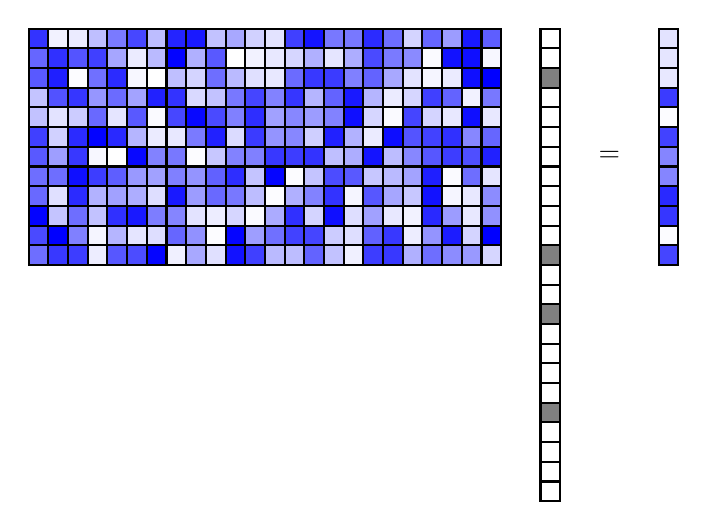
\begin{tikzpicture}
[draw=black, line width=0.75pt,
entry/.style={rectangle, draw, inner sep=0pt, minimum size=2.5mm},
symbol/.style={rectangle, draw, inner sep=0pt, minimum size=2.5mm}]

\node[entry, fill=blue!57] (x0y0) at (0.0,0.0) {};
\node[entry, fill=blue!71] (x0y1) at (0.0,0.25) {};
\node[entry, fill=blue!99] (x0y2) at (0.0,0.5) {};
\node[entry, fill=blue!59] (x0y3) at (0.0,0.75) {};
\node[entry, fill=blue!57] (x0y4) at (0.0,1.0) {};
\node[entry, fill=blue!65] (x0y5) at (0.0,1.25) {};
\node[entry, fill=blue!75] (x0y6) at (0.0,1.5) {};
\node[entry, fill=blue!24] (x0y7) at (0.0,1.75) {};
\node[entry, fill=blue!23] (x0y8) at (0.0,2.0) {};
\node[entry, fill=blue!65] (x0y9) at (0.0,2.25) {};
\node[entry, fill=blue!60] (x0y10) at (0.0,2.5) {};
\node[entry, fill=blue!80] (x0y11) at (0.0,2.75) {};

\node[entry, fill=blue!78] (x1y0) at (0.25,0.0) {};
\node[entry, fill=blue!101] (x1y1) at (0.25,0.25) {};
\node[entry, fill=blue!23] (x1y2) at (0.25,0.5) {};
\node[entry, fill=blue!12] (x1y3) at (0.25,0.75) {};
\node[entry, fill=blue!57] (x1y4) at (0.25,1.0) {};
\node[entry, fill=blue!38] (x1y5) at (0.25,1.25) {};
\node[entry, fill=blue!18] (x1y6) at (0.25,1.5) {};
\node[entry, fill=blue!11] (x1y7) at (0.25,1.75) {};
\node[entry, fill=blue!68] (x1y8) at (0.25,2.0) {};
\node[entry, fill=blue!88] (x1y9) at (0.25,2.25) {};
\node[entry, fill=blue!81] (x1y10) at (0.25,2.5) {};
\node[entry, fill=blue!5] (x1y11) at (0.25,2.75) {};

\node[entry, fill=blue!76] (x2y0) at (0.5,0.0) {};
\node[entry, fill=blue!50] (x2y1) at (0.5,0.25) {};
\node[entry, fill=blue!57] (x2y2) at (0.5,0.5) {};
\node[entry, fill=blue!83] (x2y3) at (0.5,0.75) {};
\node[entry, fill=blue!94] (x2y4) at (0.5,1.0) {};
\node[entry, fill=blue!78] (x2y5) at (0.5,1.25) {};
\node[entry, fill=blue!83] (x2y6) at (0.5,1.5) {};
\node[entry, fill=blue!20] (x2y7) at (0.5,1.75) {};
\node[entry, fill=blue!79] (x2y8) at (0.5,2.0) {};
\node[entry, fill=blue!1] (x2y9) at (0.5,2.25) {};
\node[entry, fill=blue!67] (x2y10) at (0.5,2.5) {};
\node[entry, fill=blue!8] (x2y11) at (0.5,2.75) {};

\node[entry, fill=blue!7] (x3y0) at (0.75,0.0) {};
\node[entry, fill=blue!4] (x3y1) at (0.75,0.25) {};
\node[entry, fill=blue!24] (x3y2) at (0.75,0.5) {};
\node[entry, fill=blue!30] (x3y3) at (0.75,0.75) {};
\node[entry, fill=blue!76] (x3y4) at (0.75,1.0) {};
\node[entry, fill=blue!3] (x3y5) at (0.75,1.25) {};
\node[entry, fill=blue!99] (x3y6) at (0.75,1.5) {};
\node[entry, fill=blue!59] (x3y7) at (0.75,1.75) {};
\node[entry, fill=blue!41] (x3y8) at (0.75,2.0) {};
\node[entry, fill=blue!56] (x3y9) at (0.75,2.25) {};
\node[entry, fill=blue!75] (x3y10) at (0.75,2.5) {};
\node[entry, fill=blue!25] (x3y11) at (0.75,2.75) {};

\node[entry, fill=blue!66] (x4y0) at (1.0,0.0) {};
\node[entry, fill=blue!29] (x4y1) at (1.0,0.25) {};
\node[entry, fill=blue!81] (x4y2) at (1.0,0.5) {};
\node[entry, fill=blue!37] (x4y3) at (1.0,0.75) {};
\node[entry, fill=blue!63] (x4y4) at (1.0,1.0) {};
\node[entry, fill=blue!0] (x4y5) at (1.0,1.25) {};
\node[entry, fill=blue!84] (x4y6) at (1.0,1.5) {};
\node[entry, fill=blue!10] (x4y7) at (1.0,1.75) {};
\node[entry, fill=blue!58] (x4y8) at (1.0,2.0) {};
\node[entry, fill=blue!83] (x4y9) at (1.0,2.25) {};
\node[entry, fill=blue!35] (x4y10) at (1.0,2.5) {};
\node[entry, fill=blue!52] (x4y11) at (1.0,2.75) {};

\node[entry, fill=blue!70] (x5y0) at (1.25,0.0) {};
\node[entry, fill=blue!10] (x5y1) at (1.25,0.25) {};
\node[entry, fill=blue!90] (x5y2) at (1.25,0.5) {};
\node[entry, fill=blue!32] (x5y3) at (1.25,0.75) {};
\node[entry, fill=blue!40] (x5y4) at (1.25,1.0) {};
\node[entry, fill=blue!97] (x5y5) at (1.25,1.25) {};
\node[entry, fill=blue!29] (x5y6) at (1.25,1.5) {};
\node[entry, fill=blue!65] (x5y7) at (1.25,1.75) {};
\node[entry, fill=blue!36] (x5y8) at (1.25,2.0) {};
\node[entry, fill=blue!3] (x5y9) at (1.25,2.25) {};
\node[entry, fill=blue!8] (x5y10) at (1.25,2.5) {};
\node[entry, fill=blue!72] (x5y11) at (1.25,2.75) {};

\node[entry, fill=blue!98] (x6y0) at (1.5,0.0) {};
\node[entry, fill=blue!13] (x6y1) at (1.5,0.25) {};
\node[entry, fill=blue!51] (x6y2) at (1.5,0.5) {};
\node[entry, fill=blue!13] (x6y3) at (1.5,0.75) {};
\node[entry, fill=blue!37] (x6y4) at (1.5,1.0) {};
\node[entry, fill=blue!49] (x6y5) at (1.5,1.25) {};
\node[entry, fill=blue!8] (x6y6) at (1.5,1.5) {};
\node[entry, fill=blue!2] (x6y7) at (1.5,1.75) {};
\node[entry, fill=blue!87] (x6y8) at (1.5,2.0) {};
\node[entry, fill=blue!0] (x6y9) at (1.5,2.25) {};
\node[entry, fill=blue!27] (x6y10) at (1.5,2.5) {};
\node[entry, fill=blue!26] (x6y11) at (1.5,2.75) {};

\node[entry, fill=blue!6] (x7y0) at (1.75,0.0) {};
\node[entry, fill=blue!60] (x7y1) at (1.75,0.25) {};
\node[entry, fill=blue!48] (x7y2) at (1.75,0.5) {};
\node[entry, fill=blue!90] (x7y3) at (1.75,0.75) {};
\node[entry, fill=blue!50] (x7y4) at (1.75,1.0) {};
\node[entry, fill=blue!53] (x7y5) at (1.75,1.25) {};
\node[entry, fill=blue!9] (x7y6) at (1.75,1.5) {};
\node[entry, fill=blue!72] (x7y7) at (1.75,1.75) {};
\node[entry, fill=blue!80] (x7y8) at (1.75,2.0) {};
\node[entry, fill=blue!25] (x7y9) at (1.75,2.25) {};
\node[entry, fill=blue!99] (x7y10) at (1.75,2.5) {};
\node[entry, fill=blue!86] (x7y11) at (1.75,2.75) {};

\node[entry, fill=blue!34] (x8y0) at (2.0,0.0) {};
\node[entry, fill=blue!43] (x8y1) at (2.0,0.25) {};
\node[entry, fill=blue!11] (x8y2) at (2.0,0.5) {};
\node[entry, fill=blue!39] (x8y3) at (2.0,0.75) {};
\node[entry, fill=blue!42] (x8y4) at (2.0,1.0) {};
\node[entry, fill=blue!1] (x8y5) at (2.0,1.25) {};
\node[entry, fill=blue!52] (x8y6) at (2.0,1.5) {};
\node[entry, fill=blue!97] (x8y7) at (2.0,1.75) {};
\node[entry, fill=blue!15] (x8y8) at (2.0,2.0) {};
\node[entry, fill=blue!17] (x8y9) at (2.0,2.25) {};
\node[entry, fill=blue!31] (x8y10) at (2.0,2.5) {};
\node[entry, fill=blue!90] (x8y11) at (2.0,2.75) {};

\node[entry, fill=blue!12] (x9y0) at (2.25,0.0) {};
\node[entry, fill=blue!1] (x9y1) at (2.25,0.25) {};
\node[entry, fill=blue!7] (x9y2) at (2.25,0.5) {};
\node[entry, fill=blue!59] (x9y3) at (2.25,0.75) {};
\node[entry, fill=blue!62] (x9y4) at (2.25,1.0) {};
\node[entry, fill=blue!22] (x9y5) at (2.25,1.25) {};
\node[entry, fill=blue!87] (x9y6) at (2.25,1.5) {};
\node[entry, fill=blue!71] (x9y7) at (2.25,1.75) {};
\node[entry, fill=blue!24] (x9y8) at (2.25,2.0) {};
\node[entry, fill=blue!57] (x9y9) at (2.25,2.25) {};
\node[entry, fill=blue!65] (x9y10) at (2.25,2.5) {};
\node[entry, fill=blue!24] (x9y11) at (2.25,2.75) {};

\node[entry, fill=blue!93] (x10y0) at (2.5,0.0) {};
\node[entry, fill=blue!98] (x10y1) at (2.5,0.25) {};
\node[entry, fill=blue!16] (x10y2) at (2.5,0.5) {};
\node[entry, fill=blue!53] (x10y3) at (2.5,0.75) {};
\node[entry, fill=blue!82] (x10y4) at (2.5,1.0) {};
\node[entry, fill=blue!49] (x10y5) at (2.5,1.25) {};
\node[entry, fill=blue!14] (x10y6) at (2.5,1.5) {};
\node[entry, fill=blue!50] (x10y7) at (2.5,1.75) {};
\node[entry, fill=blue!53] (x10y8) at (2.5,2.0) {};
\node[entry, fill=blue!27] (x10y9) at (2.5,2.25) {};
\node[entry, fill=blue!0] (x10y10) at (2.5,2.5) {};
\node[entry, fill=blue!34] (x10y11) at (2.5,2.75) {};

\node[entry, fill=blue!75] (x11y0) at (2.75,0.0) {};
\node[entry, fill=blue!38] (x11y1) at (2.75,0.25) {};
\node[entry, fill=blue!2] (x11y2) at (2.75,0.5) {};
\node[entry, fill=blue!26] (x11y3) at (2.75,0.75) {};
\node[entry, fill=blue!23] (x11y4) at (2.75,1.0) {};
\node[entry, fill=blue!50] (x11y5) at (2.75,1.25) {};
\node[entry, fill=blue!77] (x11y6) at (2.75,1.5) {};
\node[entry, fill=blue!82] (x11y7) at (2.75,1.75) {};
\node[entry, fill=blue!73] (x11y8) at (2.75,2.0) {};
\node[entry, fill=blue!12] (x11y9) at (2.75,2.25) {};
\node[entry, fill=blue!5] (x11y10) at (2.75,2.5) {};
\node[entry, fill=blue!18] (x11y11) at (2.75,2.75) {};

\node[entry, fill=blue!27] (x12y0) at (3.0,0.0) {};
\node[entry, fill=blue!56] (x12y1) at (3.0,0.25) {};
\node[entry, fill=blue!33] (x12y2) at (3.0,0.5) {};
\node[entry, fill=blue!1] (x12y3) at (3.0,0.75) {};
\node[entry, fill=blue!98] (x12y4) at (3.0,1.0) {};
\node[entry, fill=blue!78] (x12y5) at (3.0,1.25) {};
\node[entry, fill=blue!42] (x12y6) at (3.0,1.5) {};
\node[entry, fill=blue!37] (x12y7) at (3.0,1.75) {};
\node[entry, fill=blue!49] (x12y8) at (3.0,2.0) {};
\node[entry, fill=blue!9] (x12y9) at (3.0,2.25) {};
\node[entry, fill=blue!9] (x12y10) at (3.0,2.5) {};
\node[entry, fill=blue!11] (x12y11) at (3.0,2.75) {};

\node[entry, fill=blue!26] (x13y0) at (3.25,0.0) {};
\node[entry, fill=blue!74] (x13y1) at (3.25,0.25) {};
\node[entry, fill=blue!81] (x13y2) at (3.25,0.5) {};
\node[entry, fill=blue!31] (x13y3) at (3.25,0.75) {};
\node[entry, fill=blue!1] (x13y4) at (3.25,1.0) {};
\node[entry, fill=blue!76] (x13y5) at (3.25,1.25) {};
\node[entry, fill=blue!47] (x13y6) at (3.25,1.5) {};
\node[entry, fill=blue!47] (x13y7) at (3.25,1.75) {};
\node[entry, fill=blue!79] (x13y8) at (3.25,2.0) {};
\node[entry, fill=blue!58] (x13y9) at (3.25,2.25) {};
\node[entry, fill=blue!16] (x13y10) at (3.25,2.5) {};
\node[entry, fill=blue!75] (x13y11) at (3.25,2.75) {};

\node[entry, fill=blue!61] (x14y0) at (3.5,0.0) {};
\node[entry, fill=blue!73] (x14y1) at (3.5,0.25) {};
\node[entry, fill=blue!17] (x14y2) at (3.5,0.5) {};
\node[entry, fill=blue!49] (x14y3) at (3.5,0.75) {};
\node[entry, fill=blue!23] (x14y4) at (3.5,1.0) {};
\node[entry, fill=blue!80] (x14y5) at (3.5,1.25) {};
\node[entry, fill=blue!19] (x14y6) at (3.5,1.5) {};
\node[entry, fill=blue!39] (x14y7) at (3.5,1.75) {};
\node[entry, fill=blue!29] (x14y8) at (3.5,2.0) {};
\node[entry, fill=blue!78] (x14y9) at (3.5,2.25) {};
\node[entry, fill=blue!31] (x14y10) at (3.5,2.5) {};
\node[entry, fill=blue!92] (x14y11) at (3.5,2.75) {};

\node[entry, fill=blue!24] (x15y0) at (3.75,0.0) {};
\node[entry, fill=blue!20] (x15y1) at (3.75,0.25) {};
\node[entry, fill=blue!94] (x15y2) at (3.75,0.5) {};
\node[entry, fill=blue!80] (x15y3) at (3.75,0.75) {};
\node[entry, fill=blue!70] (x15y4) at (3.75,1.0) {};
\node[entry, fill=blue!25] (x15y5) at (3.75,1.25) {};
\node[entry, fill=blue!87] (x15y6) at (3.75,1.5) {};
\node[entry, fill=blue!49] (x15y7) at (3.75,1.75) {};
\node[entry, fill=blue!61] (x15y8) at (3.75,2.0) {};
\node[entry, fill=blue!77] (x15y9) at (3.75,2.25) {};
\node[entry, fill=blue!10] (x15y10) at (3.75,2.5) {};
\node[entry, fill=blue!53] (x15y11) at (3.75,2.75) {};

\node[entry, fill=blue!6] (x16y0) at (4.0,0.0) {};
\node[entry, fill=blue!13] (x16y1) at (4.0,0.25) {};
\node[entry, fill=blue!13] (x16y2) at (4.0,0.5) {};
\node[entry, fill=blue!4] (x16y3) at (4.0,0.75) {};
\node[entry, fill=blue!65] (x16y4) at (4.0,1.0) {};
\node[entry, fill=blue!32] (x16y5) at (4.0,1.25) {};
\node[entry, fill=blue!30] (x16y6) at (4.0,1.5) {};
\node[entry, fill=blue!94] (x16y7) at (4.0,1.75) {};
\node[entry, fill=blue!90] (x16y8) at (4.0,2.0) {};
\node[entry, fill=blue!50] (x16y9) at (4.0,2.25) {};
\node[entry, fill=blue!32] (x16y10) at (4.0,2.5) {};
\node[entry, fill=blue!53] (x16y11) at (4.0,2.75) {};

\node[entry, fill=blue!76] (x17y0) at (4.25,0.0) {};
\node[entry, fill=blue!62] (x17y1) at (4.25,0.25) {};
\node[entry, fill=blue!37] (x17y2) at (4.25,0.5) {};
\node[entry, fill=blue!66] (x17y3) at (4.25,0.75) {};
\node[entry, fill=blue!22] (x17y4) at (4.25,1.0) {};
\node[entry, fill=blue!92] (x17y5) at (4.25,1.25) {};
\node[entry, fill=blue!8] (x17y6) at (4.25,1.5) {};
\node[entry, fill=blue!16] (x17y7) at (4.25,1.75) {};
\node[entry, fill=blue!29] (x17y8) at (4.25,2.0) {};
\node[entry, fill=blue!61] (x17y9) at (4.25,2.25) {};
\node[entry, fill=blue!71] (x17y10) at (4.25,2.5) {};
\node[entry, fill=blue!83] (x17y11) at (4.25,2.75) {};

\node[entry, fill=blue!78] (x18y0) at (4.5,0.0) {};
\node[entry, fill=blue!78] (x18y1) at (4.5,0.25) {};
\node[entry, fill=blue!9] (x18y2) at (4.5,0.5) {};
\node[entry, fill=blue!35] (x18y3) at (4.5,0.75) {};
\node[entry, fill=blue!27] (x18y4) at (4.5,1.0) {};
\node[entry, fill=blue!26] (x18y5) at (4.5,1.25) {};
\node[entry, fill=blue!95] (x18y6) at (4.5,1.5) {};
\node[entry, fill=blue!2] (x18y7) at (4.5,1.75) {};
\node[entry, fill=blue!8] (x18y8) at (4.5,2.0) {};
\node[entry, fill=blue!34] (x18y9) at (4.5,2.25) {};
\node[entry, fill=blue!52] (x18y10) at (4.5,2.5) {};
\node[entry, fill=blue!57] (x18y11) at (4.5,2.75) {};

\node[entry, fill=blue!31] (x19y0) at (4.75,0.0) {};
\node[entry, fill=blue!7] (x19y1) at (4.75,0.25) {};
\node[entry, fill=blue!5] (x19y2) at (4.75,0.5) {};
\node[entry, fill=blue!22] (x19y3) at (4.75,0.75) {};
\node[entry, fill=blue!36] (x19y4) at (4.75,1.0) {};
\node[entry, fill=blue!47] (x19y5) at (4.75,1.25) {};
\node[entry, fill=blue!67] (x19y6) at (4.75,1.5) {};
\node[entry, fill=blue!73] (x19y7) at (4.75,1.75) {};
\node[entry, fill=blue!16] (x19y8) at (4.75,2.0) {};
\node[entry, fill=blue!11] (x19y9) at (4.75,2.25) {};
\node[entry, fill=blue!46] (x19y10) at (4.75,2.5) {};
\node[entry, fill=blue!17] (x19y11) at (4.75,2.75) {};

\node[entry, fill=blue!57] (x20y0) at (5.0,0.0) {};
\node[entry, fill=blue!42] (x20y1) at (5.0,0.25) {};
\node[entry, fill=blue!84] (x20y2) at (5.0,0.5) {};
\node[entry, fill=blue!93] (x20y3) at (5.0,0.75) {};
\node[entry, fill=blue!88] (x20y4) at (5.0,1.0) {};
\node[entry, fill=blue!66] (x20y5) at (5.0,1.25) {};
\node[entry, fill=blue!74] (x20y6) at (5.0,1.5) {};
\node[entry, fill=blue!17] (x20y7) at (5.0,1.75) {};
\node[entry, fill=blue!75] (x20y8) at (5.0,2.0) {};
\node[entry, fill=blue!4] (x20y9) at (5.0,2.25) {};
\node[entry, fill=blue!2] (x20y10) at (5.0,2.5) {};
\node[entry, fill=blue!60] (x20y11) at (5.0,2.75) {};

\node[entry, fill=blue!45] (x21y0) at (5.25,0.0) {};
\node[entry, fill=blue!89] (x21y1) at (5.25,0.25) {};
\node[entry, fill=blue!39] (x21y2) at (5.25,0.5) {};
\node[entry, fill=blue!4] (x21y3) at (5.25,0.75) {};
\node[entry, fill=blue!2] (x21y4) at (5.25,1.0) {};
\node[entry, fill=blue!76] (x21y5) at (5.25,1.25) {};
\node[entry, fill=blue!81] (x21y6) at (5.25,1.5) {};
\node[entry, fill=blue!9] (x21y7) at (5.25,1.75) {};
\node[entry, fill=blue!61] (x21y8) at (5.25,2.0) {};
\node[entry, fill=blue!8] (x21y9) at (5.25,2.25) {};
\node[entry, fill=blue!93] (x21y10) at (5.25,2.5) {};
\node[entry, fill=blue!39] (x21y11) at (5.25,2.75) {};

\node[entry, fill=blue!40] (x22y0) at (5.5,0.0) {};
\node[entry, fill=blue!17] (x22y1) at (5.5,0.25) {};
\node[entry, fill=blue!9] (x22y2) at (5.5,0.5) {};
\node[entry, fill=blue!9] (x22y3) at (5.5,0.75) {};
\node[entry, fill=blue!57] (x22y4) at (5.5,1.0) {};
\node[entry, fill=blue!69] (x22y5) at (5.5,1.25) {};
\node[entry, fill=blue!47] (x22y6) at (5.5,1.5) {};
\node[entry, fill=blue!94] (x22y7) at (5.5,1.75) {};
\node[entry, fill=blue!5] (x22y8) at (5.5,2.0) {};
\node[entry, fill=blue!94] (x22y9) at (5.5,2.25) {};
\node[entry, fill=blue!94] (x22y10) at (5.5,2.5) {};
\node[entry, fill=blue!90] (x22y11) at (5.5,2.75) {};

\node[entry, fill=blue!16] (x23y0) at (5.75,0.0) {};
\node[entry, fill=blue!101] (x23y1) at (5.75,0.25) {};
\node[entry, fill=blue!43] (x23y2) at (5.75,0.5) {};
\node[entry, fill=blue!45] (x23y3) at (5.75,0.75) {};
\node[entry, fill=blue!10] (x23y4) at (5.75,1.0) {};
\node[entry, fill=blue!87] (x23y5) at (5.75,1.25) {};
\node[entry, fill=blue!60] (x23y6) at (5.75,1.5) {};
\node[entry, fill=blue!9] (x23y7) at (5.75,1.75) {};
\node[entry, fill=blue!53] (x23y8) at (5.75,2.0) {};
\node[entry, fill=blue!101] (x23y9) at (5.75,2.25) {};
\node[entry, fill=blue!3] (x23y10) at (5.75,2.5) {};
\node[entry, fill=blue!63] (x23y11) at (5.75,2.75) {};

\node[symbol] (s01) at (6.5,-3.00) {};
\node[symbol] (s02) at (6.5,-2.75) {};
\node[symbol] (s03) at (6.5,-2.50) {};
\node[symbol] (s04) at (6.5,-2.25) {};
\node[symbol,fill=gray] (s05) at (6.5,-2.00) {};
\node[symbol] (s06) at (6.5,-1.75) {};
\node[symbol] (s07) at (6.5,-1.50) {};
\node[symbol] (s08) at (6.5,-1.25) {};
\node[symbol] (s09) at (6.5,-1.00) {};
\node[symbol,fill=gray] (s10) at (6.5,-0.75) {};
\node[symbol] (s11) at (6.5,-0.50) {};
\node[symbol] (s12) at (6.5,-0.25) {};
\node[symbol,fill=gray] (s13) at (6.5,0) {};
\node[symbol] (s14) at (6.5,0.25) {};
\node[symbol] (s15) at (6.5,0.50) {};
\node[symbol] (s16) at (6.5,0.75) {};
\node[symbol] (s17) at (6.5,1.00) {};
\node[symbol] (s18) at (6.5,1.25) {};
\node[symbol] (s19) at (6.5,1.50) {};
\node[symbol] (s20) at (6.5,1.75) {};
\node[symbol] (s21) at (6.5,2.00) {};
\node[symbol,fill=gray] (s22) at (6.5,2.25) {};
\node[symbol] (s23) at (6.5,2.50) {};
\node[symbol] (s24) at (6.5,2.75) {};

\node (equal) at (7.25,1.25) {$=$};

\node[entry, fill=blue!73] (o0) at (8.0,0.0) {};
\node[entry, fill=blue!1] (o1) at (8.0,0.25) {};
\node[entry, fill=blue!79] (o2) at (8.0,0.5) {};
\node[entry, fill=blue!84] (o3) at (8.0,0.75) {};
\node[entry, fill=blue!48] (o4) at (8.0,1.0) {};
\node[entry, fill=blue!48] (o5) at (8.0,1.25) {};
\node[entry, fill=blue!74] (o6) at (8.0,1.5) {};
\node[entry, fill=blue!1] (o7) at (8.0,1.75) {};
\node[entry, fill=blue!77] (o8) at (8.0,2.0) {};
\node[entry, fill=blue!9] (o9) at (8.0,2.25) {};
\node[entry, fill=blue!10] (o10) at (8.0,2.5) {};
\node[entry, fill=blue!11] (o11) at (8.0,2.75) {};

\end{tikzpicture}
}
\vspace{-2cm}
% % % % %
\begin{columns}
\column{.80\textwidth}
\scalebox{0.8}{\begin{tikzpicture}
  [
  font=\footnotesize, draw=black, >=stealth', line width=1.25pt,
  channel/.style={rectangle, minimum height=20mm, minimum width=15mm, draw=black, fill=blue!25, rounded corners},
  encoder/.style={rectangle, minimum height=6mm, minimum width=15mm, draw=black, fill=blue!25, rounded corners},
  decoder/.style={rectangle, minimum height=20mm, minimum width=15mm, draw=black, rounded corners},
  message/.style={rectangle, minimum height=6mm, minimum width=15mm, draw=black, fill=blue!25, rounded corners}
  ]

\foreach \e in {1,2,3,5} {
  \node[encoder] (e\e) at (2.25,3-\e) {Encoder};
}

\foreach \m in {1,2,3} {
  \node[message] (m\m) at (0.0,3-\m) {Message~${\m}$}
  edge[->] (e\m);
  \draw[<-] (m\m) -- (-1.25,3-\m);
}

\foreach \m in {5} {
  \node[message] (m\m) at (0.0,3-\m) {Message~$K$}
  edge[->] (e\m);
  \draw[<-] (m\m) -- (-1.25,3-\m);
}

\node at (0,-0.9) {$\vdots$};
\node at (2.25,-0.9) {$\vdots$};

\node[channel,align=center] (channel) at (5,0) {Multiple\\Access\\Channel};
\node[decoder,align=center] (decoder) at (7.25,0) {Joint\\Decoder};
\draw[->] (channel) -- (decoder);

\draw[->] (decoder.east) -- (8.5,0);

\draw[->] (e1.east) -- (channel);
\draw[->] (e2.east) -- (channel);
\draw[->] (e3.east) -- (channel);
\draw[->] (e5.east) -- (channel);

\end{tikzpicture}
}
\column{.15\textwidth}
\end{columns}
% % % % %
\end{frame}

% % % % % % % % % % % % % % % % % % % %

\begin{frame}
\frametitle{Abstract CS Challenge}
% % % % %
\begin{columns}
\column{0.54\textwidth}
\structure{\large Problem setting}
  \begin{itemize}
  \item Noisy compressed sensing
  \begin{equation*}
  \yv = \boldsymbol{\Phi} \sv + \zv
  \end{equation*}
  where $\sv$ is $K$ sparse
  \item $\sv$ has non-negative integer entries
  \item $\boldsymbol{\Phi}.\mathtt{shape} \approx 32,768 \times 2^{128}$
  \item $\zv$ is additive Gaussian noise
  \end{itemize}
\column{0.44\textwidth}
  \hspace{-1cm} \scalebox{0.75}{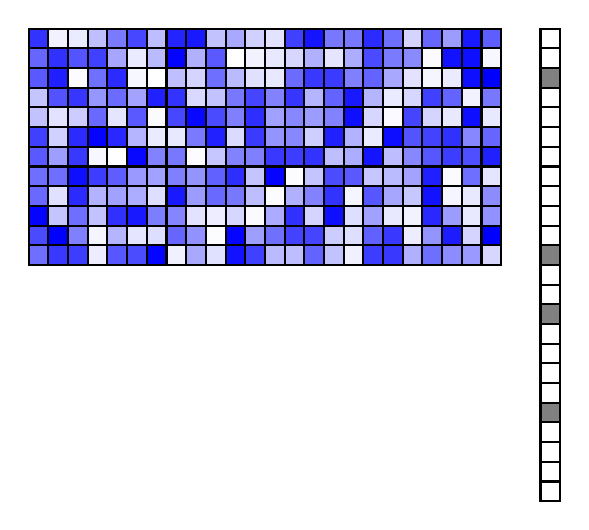
\begin{tikzpicture}
[draw=black, line width=0.75pt,
entry/.style={rectangle, draw, inner sep=0pt, minimum size=2.5mm},
symbol/.style={rectangle, draw, inner sep=0pt, minimum size=2.5mm}]

\node[entry, fill=blue!57] (x0y0) at (0.0,0.0) {};
\node[entry, fill=blue!71] (x0y1) at (0.0,0.25) {};
\node[entry, fill=blue!99] (x0y2) at (0.0,0.5) {};
\node[entry, fill=blue!59] (x0y3) at (0.0,0.75) {};
\node[entry, fill=blue!57] (x0y4) at (0.0,1.0) {};
\node[entry, fill=blue!65] (x0y5) at (0.0,1.25) {};
\node[entry, fill=blue!75] (x0y6) at (0.0,1.5) {};
\node[entry, fill=blue!24] (x0y7) at (0.0,1.75) {};
\node[entry, fill=blue!23] (x0y8) at (0.0,2.0) {};
\node[entry, fill=blue!65] (x0y9) at (0.0,2.25) {};
\node[entry, fill=blue!60] (x0y10) at (0.0,2.5) {};
\node[entry, fill=blue!80] (x0y11) at (0.0,2.75) {};

\node[entry, fill=blue!78] (x1y0) at (0.25,0.0) {};
\node[entry, fill=blue!101] (x1y1) at (0.25,0.25) {};
\node[entry, fill=blue!23] (x1y2) at (0.25,0.5) {};
\node[entry, fill=blue!12] (x1y3) at (0.25,0.75) {};
\node[entry, fill=blue!57] (x1y4) at (0.25,1.0) {};
\node[entry, fill=blue!38] (x1y5) at (0.25,1.25) {};
\node[entry, fill=blue!18] (x1y6) at (0.25,1.5) {};
\node[entry, fill=blue!11] (x1y7) at (0.25,1.75) {};
\node[entry, fill=blue!68] (x1y8) at (0.25,2.0) {};
\node[entry, fill=blue!88] (x1y9) at (0.25,2.25) {};
\node[entry, fill=blue!81] (x1y10) at (0.25,2.5) {};
\node[entry, fill=blue!5] (x1y11) at (0.25,2.75) {};

\node[entry, fill=blue!76] (x2y0) at (0.5,0.0) {};
\node[entry, fill=blue!50] (x2y1) at (0.5,0.25) {};
\node[entry, fill=blue!57] (x2y2) at (0.5,0.5) {};
\node[entry, fill=blue!83] (x2y3) at (0.5,0.75) {};
\node[entry, fill=blue!94] (x2y4) at (0.5,1.0) {};
\node[entry, fill=blue!78] (x2y5) at (0.5,1.25) {};
\node[entry, fill=blue!83] (x2y6) at (0.5,1.5) {};
\node[entry, fill=blue!20] (x2y7) at (0.5,1.75) {};
\node[entry, fill=blue!79] (x2y8) at (0.5,2.0) {};
\node[entry, fill=blue!1] (x2y9) at (0.5,2.25) {};
\node[entry, fill=blue!67] (x2y10) at (0.5,2.5) {};
\node[entry, fill=blue!8] (x2y11) at (0.5,2.75) {};

\node[entry, fill=blue!7] (x3y0) at (0.75,0.0) {};
\node[entry, fill=blue!4] (x3y1) at (0.75,0.25) {};
\node[entry, fill=blue!24] (x3y2) at (0.75,0.5) {};
\node[entry, fill=blue!30] (x3y3) at (0.75,0.75) {};
\node[entry, fill=blue!76] (x3y4) at (0.75,1.0) {};
\node[entry, fill=blue!3] (x3y5) at (0.75,1.25) {};
\node[entry, fill=blue!99] (x3y6) at (0.75,1.5) {};
\node[entry, fill=blue!59] (x3y7) at (0.75,1.75) {};
\node[entry, fill=blue!41] (x3y8) at (0.75,2.0) {};
\node[entry, fill=blue!56] (x3y9) at (0.75,2.25) {};
\node[entry, fill=blue!75] (x3y10) at (0.75,2.5) {};
\node[entry, fill=blue!25] (x3y11) at (0.75,2.75) {};

\node[entry, fill=blue!66] (x4y0) at (1.0,0.0) {};
\node[entry, fill=blue!29] (x4y1) at (1.0,0.25) {};
\node[entry, fill=blue!81] (x4y2) at (1.0,0.5) {};
\node[entry, fill=blue!37] (x4y3) at (1.0,0.75) {};
\node[entry, fill=blue!63] (x4y4) at (1.0,1.0) {};
\node[entry, fill=blue!0] (x4y5) at (1.0,1.25) {};
\node[entry, fill=blue!84] (x4y6) at (1.0,1.5) {};
\node[entry, fill=blue!10] (x4y7) at (1.0,1.75) {};
\node[entry, fill=blue!58] (x4y8) at (1.0,2.0) {};
\node[entry, fill=blue!83] (x4y9) at (1.0,2.25) {};
\node[entry, fill=blue!35] (x4y10) at (1.0,2.5) {};
\node[entry, fill=blue!52] (x4y11) at (1.0,2.75) {};

\node[entry, fill=blue!70] (x5y0) at (1.25,0.0) {};
\node[entry, fill=blue!10] (x5y1) at (1.25,0.25) {};
\node[entry, fill=blue!90] (x5y2) at (1.25,0.5) {};
\node[entry, fill=blue!32] (x5y3) at (1.25,0.75) {};
\node[entry, fill=blue!40] (x5y4) at (1.25,1.0) {};
\node[entry, fill=blue!97] (x5y5) at (1.25,1.25) {};
\node[entry, fill=blue!29] (x5y6) at (1.25,1.5) {};
\node[entry, fill=blue!65] (x5y7) at (1.25,1.75) {};
\node[entry, fill=blue!36] (x5y8) at (1.25,2.0) {};
\node[entry, fill=blue!3] (x5y9) at (1.25,2.25) {};
\node[entry, fill=blue!8] (x5y10) at (1.25,2.5) {};
\node[entry, fill=blue!72] (x5y11) at (1.25,2.75) {};

\node[entry, fill=blue!98] (x6y0) at (1.5,0.0) {};
\node[entry, fill=blue!13] (x6y1) at (1.5,0.25) {};
\node[entry, fill=blue!51] (x6y2) at (1.5,0.5) {};
\node[entry, fill=blue!13] (x6y3) at (1.5,0.75) {};
\node[entry, fill=blue!37] (x6y4) at (1.5,1.0) {};
\node[entry, fill=blue!49] (x6y5) at (1.5,1.25) {};
\node[entry, fill=blue!8] (x6y6) at (1.5,1.5) {};
\node[entry, fill=blue!2] (x6y7) at (1.5,1.75) {};
\node[entry, fill=blue!87] (x6y8) at (1.5,2.0) {};
\node[entry, fill=blue!0] (x6y9) at (1.5,2.25) {};
\node[entry, fill=blue!27] (x6y10) at (1.5,2.5) {};
\node[entry, fill=blue!26] (x6y11) at (1.5,2.75) {};

\node[entry, fill=blue!6] (x7y0) at (1.75,0.0) {};
\node[entry, fill=blue!60] (x7y1) at (1.75,0.25) {};
\node[entry, fill=blue!48] (x7y2) at (1.75,0.5) {};
\node[entry, fill=blue!90] (x7y3) at (1.75,0.75) {};
\node[entry, fill=blue!50] (x7y4) at (1.75,1.0) {};
\node[entry, fill=blue!53] (x7y5) at (1.75,1.25) {};
\node[entry, fill=blue!9] (x7y6) at (1.75,1.5) {};
\node[entry, fill=blue!72] (x7y7) at (1.75,1.75) {};
\node[entry, fill=blue!80] (x7y8) at (1.75,2.0) {};
\node[entry, fill=blue!25] (x7y9) at (1.75,2.25) {};
\node[entry, fill=blue!99] (x7y10) at (1.75,2.5) {};
\node[entry, fill=blue!86] (x7y11) at (1.75,2.75) {};

\node[entry, fill=blue!34] (x8y0) at (2.0,0.0) {};
\node[entry, fill=blue!43] (x8y1) at (2.0,0.25) {};
\node[entry, fill=blue!11] (x8y2) at (2.0,0.5) {};
\node[entry, fill=blue!39] (x8y3) at (2.0,0.75) {};
\node[entry, fill=blue!42] (x8y4) at (2.0,1.0) {};
\node[entry, fill=blue!1] (x8y5) at (2.0,1.25) {};
\node[entry, fill=blue!52] (x8y6) at (2.0,1.5) {};
\node[entry, fill=blue!97] (x8y7) at (2.0,1.75) {};
\node[entry, fill=blue!15] (x8y8) at (2.0,2.0) {};
\node[entry, fill=blue!17] (x8y9) at (2.0,2.25) {};
\node[entry, fill=blue!31] (x8y10) at (2.0,2.5) {};
\node[entry, fill=blue!90] (x8y11) at (2.0,2.75) {};

\node[entry, fill=blue!12] (x9y0) at (2.25,0.0) {};
\node[entry, fill=blue!1] (x9y1) at (2.25,0.25) {};
\node[entry, fill=blue!7] (x9y2) at (2.25,0.5) {};
\node[entry, fill=blue!59] (x9y3) at (2.25,0.75) {};
\node[entry, fill=blue!62] (x9y4) at (2.25,1.0) {};
\node[entry, fill=blue!22] (x9y5) at (2.25,1.25) {};
\node[entry, fill=blue!87] (x9y6) at (2.25,1.5) {};
\node[entry, fill=blue!71] (x9y7) at (2.25,1.75) {};
\node[entry, fill=blue!24] (x9y8) at (2.25,2.0) {};
\node[entry, fill=blue!57] (x9y9) at (2.25,2.25) {};
\node[entry, fill=blue!65] (x9y10) at (2.25,2.5) {};
\node[entry, fill=blue!24] (x9y11) at (2.25,2.75) {};

\node[entry, fill=blue!93] (x10y0) at (2.5,0.0) {};
\node[entry, fill=blue!98] (x10y1) at (2.5,0.25) {};
\node[entry, fill=blue!16] (x10y2) at (2.5,0.5) {};
\node[entry, fill=blue!53] (x10y3) at (2.5,0.75) {};
\node[entry, fill=blue!82] (x10y4) at (2.5,1.0) {};
\node[entry, fill=blue!49] (x10y5) at (2.5,1.25) {};
\node[entry, fill=blue!14] (x10y6) at (2.5,1.5) {};
\node[entry, fill=blue!50] (x10y7) at (2.5,1.75) {};
\node[entry, fill=blue!53] (x10y8) at (2.5,2.0) {};
\node[entry, fill=blue!27] (x10y9) at (2.5,2.25) {};
\node[entry, fill=blue!0] (x10y10) at (2.5,2.5) {};
\node[entry, fill=blue!34] (x10y11) at (2.5,2.75) {};

\node[entry, fill=blue!75] (x11y0) at (2.75,0.0) {};
\node[entry, fill=blue!38] (x11y1) at (2.75,0.25) {};
\node[entry, fill=blue!2] (x11y2) at (2.75,0.5) {};
\node[entry, fill=blue!26] (x11y3) at (2.75,0.75) {};
\node[entry, fill=blue!23] (x11y4) at (2.75,1.0) {};
\node[entry, fill=blue!50] (x11y5) at (2.75,1.25) {};
\node[entry, fill=blue!77] (x11y6) at (2.75,1.5) {};
\node[entry, fill=blue!82] (x11y7) at (2.75,1.75) {};
\node[entry, fill=blue!73] (x11y8) at (2.75,2.0) {};
\node[entry, fill=blue!12] (x11y9) at (2.75,2.25) {};
\node[entry, fill=blue!5] (x11y10) at (2.75,2.5) {};
\node[entry, fill=blue!18] (x11y11) at (2.75,2.75) {};

\node[entry, fill=blue!27] (x12y0) at (3.0,0.0) {};
\node[entry, fill=blue!56] (x12y1) at (3.0,0.25) {};
\node[entry, fill=blue!33] (x12y2) at (3.0,0.5) {};
\node[entry, fill=blue!1] (x12y3) at (3.0,0.75) {};
\node[entry, fill=blue!98] (x12y4) at (3.0,1.0) {};
\node[entry, fill=blue!78] (x12y5) at (3.0,1.25) {};
\node[entry, fill=blue!42] (x12y6) at (3.0,1.5) {};
\node[entry, fill=blue!37] (x12y7) at (3.0,1.75) {};
\node[entry, fill=blue!49] (x12y8) at (3.0,2.0) {};
\node[entry, fill=blue!9] (x12y9) at (3.0,2.25) {};
\node[entry, fill=blue!9] (x12y10) at (3.0,2.5) {};
\node[entry, fill=blue!11] (x12y11) at (3.0,2.75) {};

\node[entry, fill=blue!26] (x13y0) at (3.25,0.0) {};
\node[entry, fill=blue!74] (x13y1) at (3.25,0.25) {};
\node[entry, fill=blue!81] (x13y2) at (3.25,0.5) {};
\node[entry, fill=blue!31] (x13y3) at (3.25,0.75) {};
\node[entry, fill=blue!1] (x13y4) at (3.25,1.0) {};
\node[entry, fill=blue!76] (x13y5) at (3.25,1.25) {};
\node[entry, fill=blue!47] (x13y6) at (3.25,1.5) {};
\node[entry, fill=blue!47] (x13y7) at (3.25,1.75) {};
\node[entry, fill=blue!79] (x13y8) at (3.25,2.0) {};
\node[entry, fill=blue!58] (x13y9) at (3.25,2.25) {};
\node[entry, fill=blue!16] (x13y10) at (3.25,2.5) {};
\node[entry, fill=blue!75] (x13y11) at (3.25,2.75) {};

\node[entry, fill=blue!61] (x14y0) at (3.5,0.0) {};
\node[entry, fill=blue!73] (x14y1) at (3.5,0.25) {};
\node[entry, fill=blue!17] (x14y2) at (3.5,0.5) {};
\node[entry, fill=blue!49] (x14y3) at (3.5,0.75) {};
\node[entry, fill=blue!23] (x14y4) at (3.5,1.0) {};
\node[entry, fill=blue!80] (x14y5) at (3.5,1.25) {};
\node[entry, fill=blue!19] (x14y6) at (3.5,1.5) {};
\node[entry, fill=blue!39] (x14y7) at (3.5,1.75) {};
\node[entry, fill=blue!29] (x14y8) at (3.5,2.0) {};
\node[entry, fill=blue!78] (x14y9) at (3.5,2.25) {};
\node[entry, fill=blue!31] (x14y10) at (3.5,2.5) {};
\node[entry, fill=blue!92] (x14y11) at (3.5,2.75) {};

\node[entry, fill=blue!24] (x15y0) at (3.75,0.0) {};
\node[entry, fill=blue!20] (x15y1) at (3.75,0.25) {};
\node[entry, fill=blue!94] (x15y2) at (3.75,0.5) {};
\node[entry, fill=blue!80] (x15y3) at (3.75,0.75) {};
\node[entry, fill=blue!70] (x15y4) at (3.75,1.0) {};
\node[entry, fill=blue!25] (x15y5) at (3.75,1.25) {};
\node[entry, fill=blue!87] (x15y6) at (3.75,1.5) {};
\node[entry, fill=blue!49] (x15y7) at (3.75,1.75) {};
\node[entry, fill=blue!61] (x15y8) at (3.75,2.0) {};
\node[entry, fill=blue!77] (x15y9) at (3.75,2.25) {};
\node[entry, fill=blue!10] (x15y10) at (3.75,2.5) {};
\node[entry, fill=blue!53] (x15y11) at (3.75,2.75) {};

\node[entry, fill=blue!6] (x16y0) at (4.0,0.0) {};
\node[entry, fill=blue!13] (x16y1) at (4.0,0.25) {};
\node[entry, fill=blue!13] (x16y2) at (4.0,0.5) {};
\node[entry, fill=blue!4] (x16y3) at (4.0,0.75) {};
\node[entry, fill=blue!65] (x16y4) at (4.0,1.0) {};
\node[entry, fill=blue!32] (x16y5) at (4.0,1.25) {};
\node[entry, fill=blue!30] (x16y6) at (4.0,1.5) {};
\node[entry, fill=blue!94] (x16y7) at (4.0,1.75) {};
\node[entry, fill=blue!90] (x16y8) at (4.0,2.0) {};
\node[entry, fill=blue!50] (x16y9) at (4.0,2.25) {};
\node[entry, fill=blue!32] (x16y10) at (4.0,2.5) {};
\node[entry, fill=blue!53] (x16y11) at (4.0,2.75) {};

\node[entry, fill=blue!76] (x17y0) at (4.25,0.0) {};
\node[entry, fill=blue!62] (x17y1) at (4.25,0.25) {};
\node[entry, fill=blue!37] (x17y2) at (4.25,0.5) {};
\node[entry, fill=blue!66] (x17y3) at (4.25,0.75) {};
\node[entry, fill=blue!22] (x17y4) at (4.25,1.0) {};
\node[entry, fill=blue!92] (x17y5) at (4.25,1.25) {};
\node[entry, fill=blue!8] (x17y6) at (4.25,1.5) {};
\node[entry, fill=blue!16] (x17y7) at (4.25,1.75) {};
\node[entry, fill=blue!29] (x17y8) at (4.25,2.0) {};
\node[entry, fill=blue!61] (x17y9) at (4.25,2.25) {};
\node[entry, fill=blue!71] (x17y10) at (4.25,2.5) {};
\node[entry, fill=blue!83] (x17y11) at (4.25,2.75) {};

\node[entry, fill=blue!78] (x18y0) at (4.5,0.0) {};
\node[entry, fill=blue!78] (x18y1) at (4.5,0.25) {};
\node[entry, fill=blue!9] (x18y2) at (4.5,0.5) {};
\node[entry, fill=blue!35] (x18y3) at (4.5,0.75) {};
\node[entry, fill=blue!27] (x18y4) at (4.5,1.0) {};
\node[entry, fill=blue!26] (x18y5) at (4.5,1.25) {};
\node[entry, fill=blue!95] (x18y6) at (4.5,1.5) {};
\node[entry, fill=blue!2] (x18y7) at (4.5,1.75) {};
\node[entry, fill=blue!8] (x18y8) at (4.5,2.0) {};
\node[entry, fill=blue!34] (x18y9) at (4.5,2.25) {};
\node[entry, fill=blue!52] (x18y10) at (4.5,2.5) {};
\node[entry, fill=blue!57] (x18y11) at (4.5,2.75) {};

\node[entry, fill=blue!31] (x19y0) at (4.75,0.0) {};
\node[entry, fill=blue!7] (x19y1) at (4.75,0.25) {};
\node[entry, fill=blue!5] (x19y2) at (4.75,0.5) {};
\node[entry, fill=blue!22] (x19y3) at (4.75,0.75) {};
\node[entry, fill=blue!36] (x19y4) at (4.75,1.0) {};
\node[entry, fill=blue!47] (x19y5) at (4.75,1.25) {};
\node[entry, fill=blue!67] (x19y6) at (4.75,1.5) {};
\node[entry, fill=blue!73] (x19y7) at (4.75,1.75) {};
\node[entry, fill=blue!16] (x19y8) at (4.75,2.0) {};
\node[entry, fill=blue!11] (x19y9) at (4.75,2.25) {};
\node[entry, fill=blue!46] (x19y10) at (4.75,2.5) {};
\node[entry, fill=blue!17] (x19y11) at (4.75,2.75) {};

\node[entry, fill=blue!57] (x20y0) at (5.0,0.0) {};
\node[entry, fill=blue!42] (x20y1) at (5.0,0.25) {};
\node[entry, fill=blue!84] (x20y2) at (5.0,0.5) {};
\node[entry, fill=blue!93] (x20y3) at (5.0,0.75) {};
\node[entry, fill=blue!88] (x20y4) at (5.0,1.0) {};
\node[entry, fill=blue!66] (x20y5) at (5.0,1.25) {};
\node[entry, fill=blue!74] (x20y6) at (5.0,1.5) {};
\node[entry, fill=blue!17] (x20y7) at (5.0,1.75) {};
\node[entry, fill=blue!75] (x20y8) at (5.0,2.0) {};
\node[entry, fill=blue!4] (x20y9) at (5.0,2.25) {};
\node[entry, fill=blue!2] (x20y10) at (5.0,2.5) {};
\node[entry, fill=blue!60] (x20y11) at (5.0,2.75) {};

\node[entry, fill=blue!45] (x21y0) at (5.25,0.0) {};
\node[entry, fill=blue!89] (x21y1) at (5.25,0.25) {};
\node[entry, fill=blue!39] (x21y2) at (5.25,0.5) {};
\node[entry, fill=blue!4] (x21y3) at (5.25,0.75) {};
\node[entry, fill=blue!2] (x21y4) at (5.25,1.0) {};
\node[entry, fill=blue!76] (x21y5) at (5.25,1.25) {};
\node[entry, fill=blue!81] (x21y6) at (5.25,1.5) {};
\node[entry, fill=blue!9] (x21y7) at (5.25,1.75) {};
\node[entry, fill=blue!61] (x21y8) at (5.25,2.0) {};
\node[entry, fill=blue!8] (x21y9) at (5.25,2.25) {};
\node[entry, fill=blue!93] (x21y10) at (5.25,2.5) {};
\node[entry, fill=blue!39] (x21y11) at (5.25,2.75) {};

\node[entry, fill=blue!40] (x22y0) at (5.5,0.0) {};
\node[entry, fill=blue!17] (x22y1) at (5.5,0.25) {};
\node[entry, fill=blue!9] (x22y2) at (5.5,0.5) {};
\node[entry, fill=blue!9] (x22y3) at (5.5,0.75) {};
\node[entry, fill=blue!57] (x22y4) at (5.5,1.0) {};
\node[entry, fill=blue!69] (x22y5) at (5.5,1.25) {};
\node[entry, fill=blue!47] (x22y6) at (5.5,1.5) {};
\node[entry, fill=blue!94] (x22y7) at (5.5,1.75) {};
\node[entry, fill=blue!5] (x22y8) at (5.5,2.0) {};
\node[entry, fill=blue!94] (x22y9) at (5.5,2.25) {};
\node[entry, fill=blue!94] (x22y10) at (5.5,2.5) {};
\node[entry, fill=blue!90] (x22y11) at (5.5,2.75) {};

\node[entry, fill=blue!16] (x23y0) at (5.75,0.0) {};
\node[entry, fill=blue!101] (x23y1) at (5.75,0.25) {};
\node[entry, fill=blue!43] (x23y2) at (5.75,0.5) {};
\node[entry, fill=blue!45] (x23y3) at (5.75,0.75) {};
\node[entry, fill=blue!10] (x23y4) at (5.75,1.0) {};
\node[entry, fill=blue!87] (x23y5) at (5.75,1.25) {};
\node[entry, fill=blue!60] (x23y6) at (5.75,1.5) {};
\node[entry, fill=blue!9] (x23y7) at (5.75,1.75) {};
\node[entry, fill=blue!53] (x23y8) at (5.75,2.0) {};
\node[entry, fill=blue!101] (x23y9) at (5.75,2.25) {};
\node[entry, fill=blue!3] (x23y10) at (5.75,2.5) {};
\node[entry, fill=blue!63] (x23y11) at (5.75,2.75) {};

\node[symbol] (s01) at (6.5,-3.00) {};
\node[symbol] (s02) at (6.5,-2.75) {};
\node[symbol] (s03) at (6.5,-2.50) {};
\node[symbol] (s04) at (6.5,-2.25) {};
\node[symbol,fill=gray] (s05) at (6.5,-2.00) {};
\node[symbol] (s06) at (6.5,-1.75) {};
\node[symbol] (s07) at (6.5,-1.50) {};
\node[symbol] (s08) at (6.5,-1.25) {};
\node[symbol] (s09) at (6.5,-1.00) {};
\node[symbol,fill=gray] (s10) at (6.5,-0.75) {};
\node[symbol] (s11) at (6.5,-0.50) {};
\node[symbol] (s12) at (6.5,-0.25) {};
\node[symbol,fill=gray] (s13) at (6.5,0) {};
\node[symbol] (s14) at (6.5,0.25) {};
\node[symbol] (s15) at (6.5,0.50) {};
\node[symbol] (s16) at (6.5,0.75) {};
\node[symbol] (s17) at (6.5,1.00) {};
\node[symbol] (s18) at (6.5,1.25) {};
\node[symbol] (s19) at (6.5,1.50) {};
\node[symbol] (s20) at (6.5,1.75) {};
\node[symbol] (s21) at (6.5,2.00) {};
\node[symbol,fill=gray] (s22) at (6.5,2.25) {};
\node[symbol] (s23) at (6.5,2.50) {};
\node[symbol] (s24) at (6.5,2.75) {};

\end{tikzpicture}
}
\end{columns}
% % % % %
\vfill
% % % % %
\begin{block}{Performance evaluation}
  \begin{itemize}
  \item Number of mistakes in support recovery normalized by $K$
  \item Related to the per user probability of error in MAC setting
  \end{itemize}
\end{block}
\end{frame}

% % % % % % % % % % % % % % % % % % % %

\begin{frame}
\frametitle{Abstract CS Challenge}
% % % % %
\begin{columns}
\column{0.54\textwidth}
\structure{\large Problem setting}
  \begin{itemize}
  \item Noisy compressed sensing
  \begin{equation*}
  \yv = \boldsymbol{\Phi} \sv + \zv
  \end{equation*}
  where $\sv$ is $K$ sparse
  \item $\sv$ has non-negative integer entries
  \item $\boldsymbol{\Phi}.\mathtt{shape} \approx 32,768 \times 2^{128}$
  \item $\zv$ is additive Gaussian noise
  \end{itemize}
\column{0.44\textwidth}
  \hspace{-1cm} \scalebox{0.75}{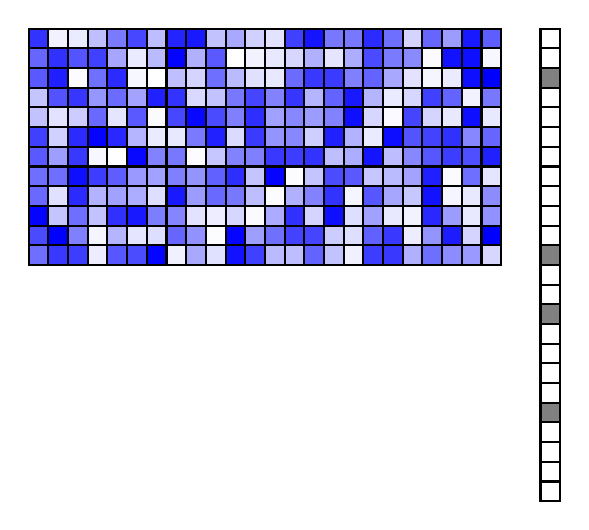
\begin{tikzpicture}
[draw=black, line width=0.75pt,
entry/.style={rectangle, draw, inner sep=0pt, minimum size=2.5mm},
symbol/.style={rectangle, draw, inner sep=0pt, minimum size=2.5mm}]

\node[entry, fill=blue!57] (x0y0) at (0.0,0.0) {};
\node[entry, fill=blue!71] (x0y1) at (0.0,0.25) {};
\node[entry, fill=blue!99] (x0y2) at (0.0,0.5) {};
\node[entry, fill=blue!59] (x0y3) at (0.0,0.75) {};
\node[entry, fill=blue!57] (x0y4) at (0.0,1.0) {};
\node[entry, fill=blue!65] (x0y5) at (0.0,1.25) {};
\node[entry, fill=blue!75] (x0y6) at (0.0,1.5) {};
\node[entry, fill=blue!24] (x0y7) at (0.0,1.75) {};
\node[entry, fill=blue!23] (x0y8) at (0.0,2.0) {};
\node[entry, fill=blue!65] (x0y9) at (0.0,2.25) {};
\node[entry, fill=blue!60] (x0y10) at (0.0,2.5) {};
\node[entry, fill=blue!80] (x0y11) at (0.0,2.75) {};

\node[entry, fill=blue!78] (x1y0) at (0.25,0.0) {};
\node[entry, fill=blue!101] (x1y1) at (0.25,0.25) {};
\node[entry, fill=blue!23] (x1y2) at (0.25,0.5) {};
\node[entry, fill=blue!12] (x1y3) at (0.25,0.75) {};
\node[entry, fill=blue!57] (x1y4) at (0.25,1.0) {};
\node[entry, fill=blue!38] (x1y5) at (0.25,1.25) {};
\node[entry, fill=blue!18] (x1y6) at (0.25,1.5) {};
\node[entry, fill=blue!11] (x1y7) at (0.25,1.75) {};
\node[entry, fill=blue!68] (x1y8) at (0.25,2.0) {};
\node[entry, fill=blue!88] (x1y9) at (0.25,2.25) {};
\node[entry, fill=blue!81] (x1y10) at (0.25,2.5) {};
\node[entry, fill=blue!5] (x1y11) at (0.25,2.75) {};

\node[entry, fill=blue!76] (x2y0) at (0.5,0.0) {};
\node[entry, fill=blue!50] (x2y1) at (0.5,0.25) {};
\node[entry, fill=blue!57] (x2y2) at (0.5,0.5) {};
\node[entry, fill=blue!83] (x2y3) at (0.5,0.75) {};
\node[entry, fill=blue!94] (x2y4) at (0.5,1.0) {};
\node[entry, fill=blue!78] (x2y5) at (0.5,1.25) {};
\node[entry, fill=blue!83] (x2y6) at (0.5,1.5) {};
\node[entry, fill=blue!20] (x2y7) at (0.5,1.75) {};
\node[entry, fill=blue!79] (x2y8) at (0.5,2.0) {};
\node[entry, fill=blue!1] (x2y9) at (0.5,2.25) {};
\node[entry, fill=blue!67] (x2y10) at (0.5,2.5) {};
\node[entry, fill=blue!8] (x2y11) at (0.5,2.75) {};

\node[entry, fill=blue!7] (x3y0) at (0.75,0.0) {};
\node[entry, fill=blue!4] (x3y1) at (0.75,0.25) {};
\node[entry, fill=blue!24] (x3y2) at (0.75,0.5) {};
\node[entry, fill=blue!30] (x3y3) at (0.75,0.75) {};
\node[entry, fill=blue!76] (x3y4) at (0.75,1.0) {};
\node[entry, fill=blue!3] (x3y5) at (0.75,1.25) {};
\node[entry, fill=blue!99] (x3y6) at (0.75,1.5) {};
\node[entry, fill=blue!59] (x3y7) at (0.75,1.75) {};
\node[entry, fill=blue!41] (x3y8) at (0.75,2.0) {};
\node[entry, fill=blue!56] (x3y9) at (0.75,2.25) {};
\node[entry, fill=blue!75] (x3y10) at (0.75,2.5) {};
\node[entry, fill=blue!25] (x3y11) at (0.75,2.75) {};

\node[entry, fill=blue!66] (x4y0) at (1.0,0.0) {};
\node[entry, fill=blue!29] (x4y1) at (1.0,0.25) {};
\node[entry, fill=blue!81] (x4y2) at (1.0,0.5) {};
\node[entry, fill=blue!37] (x4y3) at (1.0,0.75) {};
\node[entry, fill=blue!63] (x4y4) at (1.0,1.0) {};
\node[entry, fill=blue!0] (x4y5) at (1.0,1.25) {};
\node[entry, fill=blue!84] (x4y6) at (1.0,1.5) {};
\node[entry, fill=blue!10] (x4y7) at (1.0,1.75) {};
\node[entry, fill=blue!58] (x4y8) at (1.0,2.0) {};
\node[entry, fill=blue!83] (x4y9) at (1.0,2.25) {};
\node[entry, fill=blue!35] (x4y10) at (1.0,2.5) {};
\node[entry, fill=blue!52] (x4y11) at (1.0,2.75) {};

\node[entry, fill=blue!70] (x5y0) at (1.25,0.0) {};
\node[entry, fill=blue!10] (x5y1) at (1.25,0.25) {};
\node[entry, fill=blue!90] (x5y2) at (1.25,0.5) {};
\node[entry, fill=blue!32] (x5y3) at (1.25,0.75) {};
\node[entry, fill=blue!40] (x5y4) at (1.25,1.0) {};
\node[entry, fill=blue!97] (x5y5) at (1.25,1.25) {};
\node[entry, fill=blue!29] (x5y6) at (1.25,1.5) {};
\node[entry, fill=blue!65] (x5y7) at (1.25,1.75) {};
\node[entry, fill=blue!36] (x5y8) at (1.25,2.0) {};
\node[entry, fill=blue!3] (x5y9) at (1.25,2.25) {};
\node[entry, fill=blue!8] (x5y10) at (1.25,2.5) {};
\node[entry, fill=blue!72] (x5y11) at (1.25,2.75) {};

\node[entry, fill=blue!98] (x6y0) at (1.5,0.0) {};
\node[entry, fill=blue!13] (x6y1) at (1.5,0.25) {};
\node[entry, fill=blue!51] (x6y2) at (1.5,0.5) {};
\node[entry, fill=blue!13] (x6y3) at (1.5,0.75) {};
\node[entry, fill=blue!37] (x6y4) at (1.5,1.0) {};
\node[entry, fill=blue!49] (x6y5) at (1.5,1.25) {};
\node[entry, fill=blue!8] (x6y6) at (1.5,1.5) {};
\node[entry, fill=blue!2] (x6y7) at (1.5,1.75) {};
\node[entry, fill=blue!87] (x6y8) at (1.5,2.0) {};
\node[entry, fill=blue!0] (x6y9) at (1.5,2.25) {};
\node[entry, fill=blue!27] (x6y10) at (1.5,2.5) {};
\node[entry, fill=blue!26] (x6y11) at (1.5,2.75) {};

\node[entry, fill=blue!6] (x7y0) at (1.75,0.0) {};
\node[entry, fill=blue!60] (x7y1) at (1.75,0.25) {};
\node[entry, fill=blue!48] (x7y2) at (1.75,0.5) {};
\node[entry, fill=blue!90] (x7y3) at (1.75,0.75) {};
\node[entry, fill=blue!50] (x7y4) at (1.75,1.0) {};
\node[entry, fill=blue!53] (x7y5) at (1.75,1.25) {};
\node[entry, fill=blue!9] (x7y6) at (1.75,1.5) {};
\node[entry, fill=blue!72] (x7y7) at (1.75,1.75) {};
\node[entry, fill=blue!80] (x7y8) at (1.75,2.0) {};
\node[entry, fill=blue!25] (x7y9) at (1.75,2.25) {};
\node[entry, fill=blue!99] (x7y10) at (1.75,2.5) {};
\node[entry, fill=blue!86] (x7y11) at (1.75,2.75) {};

\node[entry, fill=blue!34] (x8y0) at (2.0,0.0) {};
\node[entry, fill=blue!43] (x8y1) at (2.0,0.25) {};
\node[entry, fill=blue!11] (x8y2) at (2.0,0.5) {};
\node[entry, fill=blue!39] (x8y3) at (2.0,0.75) {};
\node[entry, fill=blue!42] (x8y4) at (2.0,1.0) {};
\node[entry, fill=blue!1] (x8y5) at (2.0,1.25) {};
\node[entry, fill=blue!52] (x8y6) at (2.0,1.5) {};
\node[entry, fill=blue!97] (x8y7) at (2.0,1.75) {};
\node[entry, fill=blue!15] (x8y8) at (2.0,2.0) {};
\node[entry, fill=blue!17] (x8y9) at (2.0,2.25) {};
\node[entry, fill=blue!31] (x8y10) at (2.0,2.5) {};
\node[entry, fill=blue!90] (x8y11) at (2.0,2.75) {};

\node[entry, fill=blue!12] (x9y0) at (2.25,0.0) {};
\node[entry, fill=blue!1] (x9y1) at (2.25,0.25) {};
\node[entry, fill=blue!7] (x9y2) at (2.25,0.5) {};
\node[entry, fill=blue!59] (x9y3) at (2.25,0.75) {};
\node[entry, fill=blue!62] (x9y4) at (2.25,1.0) {};
\node[entry, fill=blue!22] (x9y5) at (2.25,1.25) {};
\node[entry, fill=blue!87] (x9y6) at (2.25,1.5) {};
\node[entry, fill=blue!71] (x9y7) at (2.25,1.75) {};
\node[entry, fill=blue!24] (x9y8) at (2.25,2.0) {};
\node[entry, fill=blue!57] (x9y9) at (2.25,2.25) {};
\node[entry, fill=blue!65] (x9y10) at (2.25,2.5) {};
\node[entry, fill=blue!24] (x9y11) at (2.25,2.75) {};

\node[entry, fill=blue!93] (x10y0) at (2.5,0.0) {};
\node[entry, fill=blue!98] (x10y1) at (2.5,0.25) {};
\node[entry, fill=blue!16] (x10y2) at (2.5,0.5) {};
\node[entry, fill=blue!53] (x10y3) at (2.5,0.75) {};
\node[entry, fill=blue!82] (x10y4) at (2.5,1.0) {};
\node[entry, fill=blue!49] (x10y5) at (2.5,1.25) {};
\node[entry, fill=blue!14] (x10y6) at (2.5,1.5) {};
\node[entry, fill=blue!50] (x10y7) at (2.5,1.75) {};
\node[entry, fill=blue!53] (x10y8) at (2.5,2.0) {};
\node[entry, fill=blue!27] (x10y9) at (2.5,2.25) {};
\node[entry, fill=blue!0] (x10y10) at (2.5,2.5) {};
\node[entry, fill=blue!34] (x10y11) at (2.5,2.75) {};

\node[entry, fill=blue!75] (x11y0) at (2.75,0.0) {};
\node[entry, fill=blue!38] (x11y1) at (2.75,0.25) {};
\node[entry, fill=blue!2] (x11y2) at (2.75,0.5) {};
\node[entry, fill=blue!26] (x11y3) at (2.75,0.75) {};
\node[entry, fill=blue!23] (x11y4) at (2.75,1.0) {};
\node[entry, fill=blue!50] (x11y5) at (2.75,1.25) {};
\node[entry, fill=blue!77] (x11y6) at (2.75,1.5) {};
\node[entry, fill=blue!82] (x11y7) at (2.75,1.75) {};
\node[entry, fill=blue!73] (x11y8) at (2.75,2.0) {};
\node[entry, fill=blue!12] (x11y9) at (2.75,2.25) {};
\node[entry, fill=blue!5] (x11y10) at (2.75,2.5) {};
\node[entry, fill=blue!18] (x11y11) at (2.75,2.75) {};

\node[entry, fill=blue!27] (x12y0) at (3.0,0.0) {};
\node[entry, fill=blue!56] (x12y1) at (3.0,0.25) {};
\node[entry, fill=blue!33] (x12y2) at (3.0,0.5) {};
\node[entry, fill=blue!1] (x12y3) at (3.0,0.75) {};
\node[entry, fill=blue!98] (x12y4) at (3.0,1.0) {};
\node[entry, fill=blue!78] (x12y5) at (3.0,1.25) {};
\node[entry, fill=blue!42] (x12y6) at (3.0,1.5) {};
\node[entry, fill=blue!37] (x12y7) at (3.0,1.75) {};
\node[entry, fill=blue!49] (x12y8) at (3.0,2.0) {};
\node[entry, fill=blue!9] (x12y9) at (3.0,2.25) {};
\node[entry, fill=blue!9] (x12y10) at (3.0,2.5) {};
\node[entry, fill=blue!11] (x12y11) at (3.0,2.75) {};

\node[entry, fill=blue!26] (x13y0) at (3.25,0.0) {};
\node[entry, fill=blue!74] (x13y1) at (3.25,0.25) {};
\node[entry, fill=blue!81] (x13y2) at (3.25,0.5) {};
\node[entry, fill=blue!31] (x13y3) at (3.25,0.75) {};
\node[entry, fill=blue!1] (x13y4) at (3.25,1.0) {};
\node[entry, fill=blue!76] (x13y5) at (3.25,1.25) {};
\node[entry, fill=blue!47] (x13y6) at (3.25,1.5) {};
\node[entry, fill=blue!47] (x13y7) at (3.25,1.75) {};
\node[entry, fill=blue!79] (x13y8) at (3.25,2.0) {};
\node[entry, fill=blue!58] (x13y9) at (3.25,2.25) {};
\node[entry, fill=blue!16] (x13y10) at (3.25,2.5) {};
\node[entry, fill=blue!75] (x13y11) at (3.25,2.75) {};

\node[entry, fill=blue!61] (x14y0) at (3.5,0.0) {};
\node[entry, fill=blue!73] (x14y1) at (3.5,0.25) {};
\node[entry, fill=blue!17] (x14y2) at (3.5,0.5) {};
\node[entry, fill=blue!49] (x14y3) at (3.5,0.75) {};
\node[entry, fill=blue!23] (x14y4) at (3.5,1.0) {};
\node[entry, fill=blue!80] (x14y5) at (3.5,1.25) {};
\node[entry, fill=blue!19] (x14y6) at (3.5,1.5) {};
\node[entry, fill=blue!39] (x14y7) at (3.5,1.75) {};
\node[entry, fill=blue!29] (x14y8) at (3.5,2.0) {};
\node[entry, fill=blue!78] (x14y9) at (3.5,2.25) {};
\node[entry, fill=blue!31] (x14y10) at (3.5,2.5) {};
\node[entry, fill=blue!92] (x14y11) at (3.5,2.75) {};

\node[entry, fill=blue!24] (x15y0) at (3.75,0.0) {};
\node[entry, fill=blue!20] (x15y1) at (3.75,0.25) {};
\node[entry, fill=blue!94] (x15y2) at (3.75,0.5) {};
\node[entry, fill=blue!80] (x15y3) at (3.75,0.75) {};
\node[entry, fill=blue!70] (x15y4) at (3.75,1.0) {};
\node[entry, fill=blue!25] (x15y5) at (3.75,1.25) {};
\node[entry, fill=blue!87] (x15y6) at (3.75,1.5) {};
\node[entry, fill=blue!49] (x15y7) at (3.75,1.75) {};
\node[entry, fill=blue!61] (x15y8) at (3.75,2.0) {};
\node[entry, fill=blue!77] (x15y9) at (3.75,2.25) {};
\node[entry, fill=blue!10] (x15y10) at (3.75,2.5) {};
\node[entry, fill=blue!53] (x15y11) at (3.75,2.75) {};

\node[entry, fill=blue!6] (x16y0) at (4.0,0.0) {};
\node[entry, fill=blue!13] (x16y1) at (4.0,0.25) {};
\node[entry, fill=blue!13] (x16y2) at (4.0,0.5) {};
\node[entry, fill=blue!4] (x16y3) at (4.0,0.75) {};
\node[entry, fill=blue!65] (x16y4) at (4.0,1.0) {};
\node[entry, fill=blue!32] (x16y5) at (4.0,1.25) {};
\node[entry, fill=blue!30] (x16y6) at (4.0,1.5) {};
\node[entry, fill=blue!94] (x16y7) at (4.0,1.75) {};
\node[entry, fill=blue!90] (x16y8) at (4.0,2.0) {};
\node[entry, fill=blue!50] (x16y9) at (4.0,2.25) {};
\node[entry, fill=blue!32] (x16y10) at (4.0,2.5) {};
\node[entry, fill=blue!53] (x16y11) at (4.0,2.75) {};

\node[entry, fill=blue!76] (x17y0) at (4.25,0.0) {};
\node[entry, fill=blue!62] (x17y1) at (4.25,0.25) {};
\node[entry, fill=blue!37] (x17y2) at (4.25,0.5) {};
\node[entry, fill=blue!66] (x17y3) at (4.25,0.75) {};
\node[entry, fill=blue!22] (x17y4) at (4.25,1.0) {};
\node[entry, fill=blue!92] (x17y5) at (4.25,1.25) {};
\node[entry, fill=blue!8] (x17y6) at (4.25,1.5) {};
\node[entry, fill=blue!16] (x17y7) at (4.25,1.75) {};
\node[entry, fill=blue!29] (x17y8) at (4.25,2.0) {};
\node[entry, fill=blue!61] (x17y9) at (4.25,2.25) {};
\node[entry, fill=blue!71] (x17y10) at (4.25,2.5) {};
\node[entry, fill=blue!83] (x17y11) at (4.25,2.75) {};

\node[entry, fill=blue!78] (x18y0) at (4.5,0.0) {};
\node[entry, fill=blue!78] (x18y1) at (4.5,0.25) {};
\node[entry, fill=blue!9] (x18y2) at (4.5,0.5) {};
\node[entry, fill=blue!35] (x18y3) at (4.5,0.75) {};
\node[entry, fill=blue!27] (x18y4) at (4.5,1.0) {};
\node[entry, fill=blue!26] (x18y5) at (4.5,1.25) {};
\node[entry, fill=blue!95] (x18y6) at (4.5,1.5) {};
\node[entry, fill=blue!2] (x18y7) at (4.5,1.75) {};
\node[entry, fill=blue!8] (x18y8) at (4.5,2.0) {};
\node[entry, fill=blue!34] (x18y9) at (4.5,2.25) {};
\node[entry, fill=blue!52] (x18y10) at (4.5,2.5) {};
\node[entry, fill=blue!57] (x18y11) at (4.5,2.75) {};

\node[entry, fill=blue!31] (x19y0) at (4.75,0.0) {};
\node[entry, fill=blue!7] (x19y1) at (4.75,0.25) {};
\node[entry, fill=blue!5] (x19y2) at (4.75,0.5) {};
\node[entry, fill=blue!22] (x19y3) at (4.75,0.75) {};
\node[entry, fill=blue!36] (x19y4) at (4.75,1.0) {};
\node[entry, fill=blue!47] (x19y5) at (4.75,1.25) {};
\node[entry, fill=blue!67] (x19y6) at (4.75,1.5) {};
\node[entry, fill=blue!73] (x19y7) at (4.75,1.75) {};
\node[entry, fill=blue!16] (x19y8) at (4.75,2.0) {};
\node[entry, fill=blue!11] (x19y9) at (4.75,2.25) {};
\node[entry, fill=blue!46] (x19y10) at (4.75,2.5) {};
\node[entry, fill=blue!17] (x19y11) at (4.75,2.75) {};

\node[entry, fill=blue!57] (x20y0) at (5.0,0.0) {};
\node[entry, fill=blue!42] (x20y1) at (5.0,0.25) {};
\node[entry, fill=blue!84] (x20y2) at (5.0,0.5) {};
\node[entry, fill=blue!93] (x20y3) at (5.0,0.75) {};
\node[entry, fill=blue!88] (x20y4) at (5.0,1.0) {};
\node[entry, fill=blue!66] (x20y5) at (5.0,1.25) {};
\node[entry, fill=blue!74] (x20y6) at (5.0,1.5) {};
\node[entry, fill=blue!17] (x20y7) at (5.0,1.75) {};
\node[entry, fill=blue!75] (x20y8) at (5.0,2.0) {};
\node[entry, fill=blue!4] (x20y9) at (5.0,2.25) {};
\node[entry, fill=blue!2] (x20y10) at (5.0,2.5) {};
\node[entry, fill=blue!60] (x20y11) at (5.0,2.75) {};

\node[entry, fill=blue!45] (x21y0) at (5.25,0.0) {};
\node[entry, fill=blue!89] (x21y1) at (5.25,0.25) {};
\node[entry, fill=blue!39] (x21y2) at (5.25,0.5) {};
\node[entry, fill=blue!4] (x21y3) at (5.25,0.75) {};
\node[entry, fill=blue!2] (x21y4) at (5.25,1.0) {};
\node[entry, fill=blue!76] (x21y5) at (5.25,1.25) {};
\node[entry, fill=blue!81] (x21y6) at (5.25,1.5) {};
\node[entry, fill=blue!9] (x21y7) at (5.25,1.75) {};
\node[entry, fill=blue!61] (x21y8) at (5.25,2.0) {};
\node[entry, fill=blue!8] (x21y9) at (5.25,2.25) {};
\node[entry, fill=blue!93] (x21y10) at (5.25,2.5) {};
\node[entry, fill=blue!39] (x21y11) at (5.25,2.75) {};

\node[entry, fill=blue!40] (x22y0) at (5.5,0.0) {};
\node[entry, fill=blue!17] (x22y1) at (5.5,0.25) {};
\node[entry, fill=blue!9] (x22y2) at (5.5,0.5) {};
\node[entry, fill=blue!9] (x22y3) at (5.5,0.75) {};
\node[entry, fill=blue!57] (x22y4) at (5.5,1.0) {};
\node[entry, fill=blue!69] (x22y5) at (5.5,1.25) {};
\node[entry, fill=blue!47] (x22y6) at (5.5,1.5) {};
\node[entry, fill=blue!94] (x22y7) at (5.5,1.75) {};
\node[entry, fill=blue!5] (x22y8) at (5.5,2.0) {};
\node[entry, fill=blue!94] (x22y9) at (5.5,2.25) {};
\node[entry, fill=blue!94] (x22y10) at (5.5,2.5) {};
\node[entry, fill=blue!90] (x22y11) at (5.5,2.75) {};

\node[entry, fill=blue!16] (x23y0) at (5.75,0.0) {};
\node[entry, fill=blue!101] (x23y1) at (5.75,0.25) {};
\node[entry, fill=blue!43] (x23y2) at (5.75,0.5) {};
\node[entry, fill=blue!45] (x23y3) at (5.75,0.75) {};
\node[entry, fill=blue!10] (x23y4) at (5.75,1.0) {};
\node[entry, fill=blue!87] (x23y5) at (5.75,1.25) {};
\node[entry, fill=blue!60] (x23y6) at (5.75,1.5) {};
\node[entry, fill=blue!9] (x23y7) at (5.75,1.75) {};
\node[entry, fill=blue!53] (x23y8) at (5.75,2.0) {};
\node[entry, fill=blue!101] (x23y9) at (5.75,2.25) {};
\node[entry, fill=blue!3] (x23y10) at (5.75,2.5) {};
\node[entry, fill=blue!63] (x23y11) at (5.75,2.75) {};

\node[symbol] (s01) at (6.5,-3.00) {};
\node[symbol] (s02) at (6.5,-2.75) {};
\node[symbol] (s03) at (6.5,-2.50) {};
\node[symbol] (s04) at (6.5,-2.25) {};
\node[symbol,fill=gray] (s05) at (6.5,-2.00) {};
\node[symbol] (s06) at (6.5,-1.75) {};
\node[symbol] (s07) at (6.5,-1.50) {};
\node[symbol] (s08) at (6.5,-1.25) {};
\node[symbol] (s09) at (6.5,-1.00) {};
\node[symbol,fill=gray] (s10) at (6.5,-0.75) {};
\node[symbol] (s11) at (6.5,-0.50) {};
\node[symbol] (s12) at (6.5,-0.25) {};
\node[symbol,fill=gray] (s13) at (6.5,0) {};
\node[symbol] (s14) at (6.5,0.25) {};
\node[symbol] (s15) at (6.5,0.50) {};
\node[symbol] (s16) at (6.5,0.75) {};
\node[symbol] (s17) at (6.5,1.00) {};
\node[symbol] (s18) at (6.5,1.25) {};
\node[symbol] (s19) at (6.5,1.50) {};
\node[symbol] (s20) at (6.5,1.75) {};
\node[symbol] (s21) at (6.5,2.00) {};
\node[symbol,fill=gray] (s22) at (6.5,2.25) {};
\node[symbol] (s23) at (6.5,2.50) {};
\node[symbol] (s24) at (6.5,2.75) {};

\end{tikzpicture}
}
\end{columns}
% % % % %
\vfill
% % % % %
\begin{alertblock}{Practical issue}
  \begin{itemize}
  \item Width of sensing matrix is huge
  \item Existing CS solvers will not execute at that scale
  \end{itemize}
\end{alertblock}
\end{frame}

% % % % % % % % % % % % % % % % % % % %

\begin{frame} \frametitle{Matrix Width \& Sparsity Undersampling Tradeoff}
\begin{center} 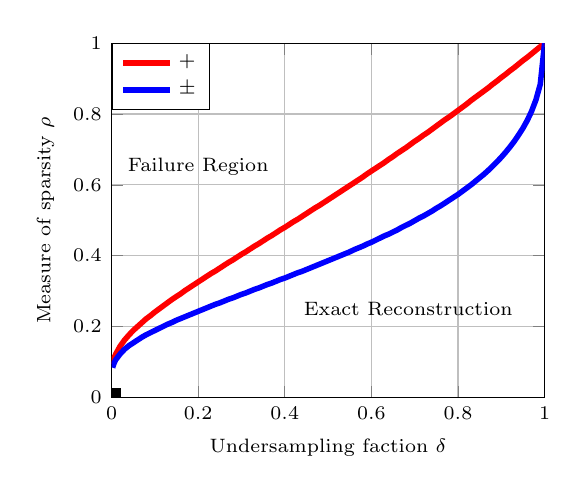
\begin{tikzpicture}

\begin{axis}[%
font=\scriptsize,
width=5.5cm,
height=4.5cm,
scale only axis,
xmin=0,
xmax=1,
xlabel={Undersampling faction $\delta$},
xmajorgrids,
ymin=0,
ymax=1,
ylabel={Measure of sparsity $\rho$},
%ylabel near ticks,
ymajorgrids,
legend style={at={(0,1)},anchor=north west,legend cell align=left,
/tikz/column 2/.style={column sep=3pt}}
]

\addplot [color=red,solid,line width=2.0pt]
  coordinates {
(0.0025,0.094) (0.005,0.107) (0.0075,0.116)
(0.01,0.123) (0.02,0.145) (0.03,0.162) (0.04,0.176) (0.05,0.189) (0.06,0.2) (0.07,0.211) (0.08,0.222) (0.09,0.231) (0.1,0.241) (0.11,0.25) (0.12,0.259) (0.13,0.268) (0.14,0.277) (0.15,0.285) (0.16,0.293) (0.17,0.302) (0.18,0.31) (0.19,0.318) (0.2,0.326) (0.21,0.334) (0.22,0.342) (0.23,0.35) (0.24,0.357) (0.25,0.365) (0.26,0.373) (0.27,0.381) (0.28,0.388) (0.29,0.396) (0.3,0.404) (0.31,0.411) (0.32,0.419) (0.33,0.427) (0.34,0.434) (0.35,0.442) (0.36,0.45) (0.37,0.457) (0.38,0.465) (0.39,0.473) (0.4,0.48) (0.41,0.488) (0.42,0.496) (0.43,0.503) (0.44,0.511) (0.45,0.519) (0.46,0.527) (0.47,0.535) (0.48,0.542) (0.49,0.55) (0.5,0.558) (0.51,0.566) (0.52,0.574) (0.53,0.582) (0.54,0.59) (0.55,0.598) (0.56,0.606) (0.57,0.614) (0.58,0.622) (0.59,0.631) (0.6,0.639) (0.61,0.647) (0.62,0.655) (0.63,0.663) (0.64,0.672) (0.65,0.68) (0.66,0.689) (0.67,0.697) (0.68,0.705) (0.69,0.714) (0.7,0.723) (0.71,0.731) (0.72,0.74) (0.73,0.748) (0.74,0.757) (0.75,0.766) (0.76,0.775) (0.77,0.784) (0.78,0.792) (0.79,0.801) (0.8,0.81) (0.81,0.819) (0.82,0.828) (0.83,0.838) (0.84,0.847) (0.85,0.856) (0.86,0.865) (0.87,0.874) (0.88,0.884) (0.89,0.893) (0.9,0.903) (0.91,0.912) (0.92,0.922) (0.93,0.931) (0.94,0.941) (0.95,0.951) (0.96,0.96) (0.97,0.97) (0.98,0.98) (0.99,0.99) (1,1)
};
\addlegendentry{$+$};

\addplot [color=blue,solid,line width=2.0pt]
  coordinates {
(0.0025,0.084) (0.005,0.094) (0.0075,0.101)
(0.01,0.107) (0.02,0.123) (0.03,0.136) (0.04,0.146) (0.05,0.154) (0.06,0.162) (0.07,0.17) (0.08,0.177) (0.09,0.183) (0.1,0.189) (0.11,0.195) (0.12,0.201) (0.13,0.207) (0.14,0.212) (0.15,0.218) (0.16,0.223) (0.17,0.228) (0.18,0.233) (0.19,0.238) (0.2,0.243) (0.21,0.248) (0.22,0.253) (0.23,0.258) (0.24,0.263) (0.25,0.267) (0.26,0.272) (0.27,0.277) (0.28,0.281) (0.29,0.286) (0.3,0.291) (0.31,0.295) (0.32,0.3) (0.33,0.305) (0.34,0.309) (0.35,0.314) (0.36,0.319) (0.37,0.323) (0.38,0.328) (0.39,0.333) (0.4,0.337) (0.41,0.342) (0.42,0.347) (0.43,0.352) (0.44,0.356) (0.45,0.361) (0.46,0.366) (0.47,0.371) (0.48,0.376) (0.49,0.381) (0.5,0.386) (0.51,0.391) (0.52,0.396) (0.53,0.401) (0.54,0.406) (0.55,0.411) (0.56,0.417) (0.57,0.422) (0.58,0.427) (0.59,0.433) (0.6,0.438) (0.61,0.444) (0.62,0.45) (0.63,0.456) (0.64,0.461) (0.65,0.467) (0.66,0.473) (0.67,0.48) (0.68,0.486) (0.69,0.492) (0.7,0.499) (0.71,0.506) (0.72,0.512) (0.73,0.519) (0.74,0.526) (0.75,0.534) (0.76,0.541) (0.77,0.549) (0.78,0.557) (0.79,0.565) (0.8,0.573) (0.81,0.582) (0.82,0.591) (0.83,0.6) (0.84,0.61) (0.85,0.62) (0.86,0.63) (0.87,0.641) (0.88,0.653) (0.89,0.665) (0.9,0.678) (0.91,0.692) (0.92,0.707) (0.93,0.723) (0.94,0.741) (0.95,0.76) (0.96,0.782) (0.97,0.808) (0.98,0.84) (0.99,0.884) (1,1)
};
\addlegendentry{$\pm$};

\node at (axis cs: 0.2, 0.65) {Failure Region};
\node at (axis cs: 0.685, 0.25) {Exact Reconstruction};

\filldraw [fill=black] (axis cs:0,0) rectangle (axis cs:0.02,0.025);

\end{axis}

\end{tikzpicture}
 \end{center}
% % % % %
\begin{columns}
\column{0.48\textwidth}
\begin{itemize}
\item Undersampling fraction \[ \delta = \frac{32,768}{2^{128}} = 2^{-113} \]
\end{itemize}
\column{0.48\textwidth}
\begin{itemize}
\item Measure of sparsity \[ \rho = \frac{256}{32,768} = 2^{-7} \]
\end{itemize}
\end{columns}
% % % % %
\end{frame}

% % % % % % % % % % % % % % % % % % % %

\begin{frame}
\frametitle{Time-Division Unsourced Random Access}
% % % % %
\begin{columns}
\column{0.54\textwidth}
\structure{\large Slot partitioning}
  \begin{itemize}
  \item Observations become
  \begin{equation*}
  \yv_{\ell} = \boldsymbol{\Phi}_{\ell} \sv_{\ell} + \zv_{\ell}
  \end{equation*}
  where $\ell$ is slot label
  \item Device gets slot based on message
  \item Channel uses divided among slots
  \end{itemize}
\column{0.44\textwidth}
  \hspace{-1cm} \scalebox{0.75}{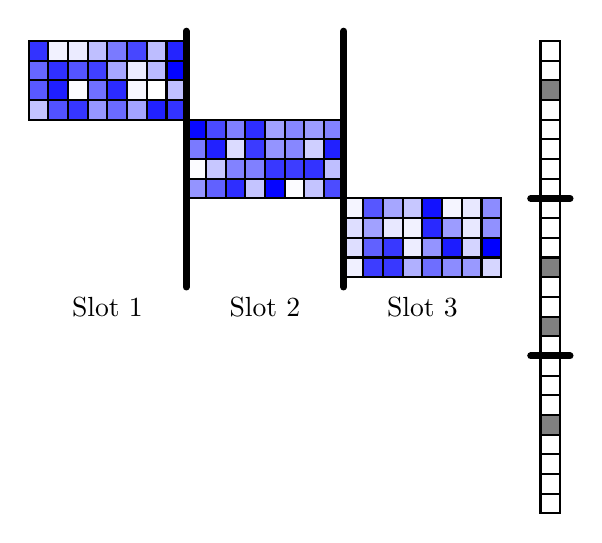
\begin{tikzpicture}
[draw=black, line width=0.75pt,
entry/.style={rectangle, draw, inner sep=0pt, minimum size=2.5mm},
symbol/.style={rectangle, draw, inner sep=0pt, minimum size=2.5mm}]

%\node[entry, fill=blue!57] (x0y0) at (0.0,0.0) {};
%\node[entry, fill=blue!71] (x0y1) at (0.0,0.25) {};
%\node[entry, fill=blue!99] (x0y2) at (0.0,0.5) {};
%\node[entry, fill=blue!59] (x0y3) at (0.0,0.75) {};
%\node[entry, fill=blue!57] (x0y4) at (0.0,1.0) {};
%\node[entry, fill=blue!65] (x0y5) at (0.0,1.25) {};
%\node[entry, fill=blue!75] (x0y6) at (0.0,1.5) {};
%\node[entry, fill=blue!24] (x0y7) at (0.0,1.75) {};
\node[entry, fill=blue!23] (x0y8) at (0.0,2.0) {};
\node[entry, fill=blue!65] (x0y9) at (0.0,2.25) {};
\node[entry, fill=blue!60] (x0y10) at (0.0,2.5) {};
\node[entry, fill=blue!80] (x0y11) at (0.0,2.75) {};

%\node[entry, fill=blue!78] (x1y0) at (0.25,0.0) {};
%\node[entry, fill=blue!101] (x1y1) at (0.25,0.25) {};
%\node[entry, fill=blue!23] (x1y2) at (0.25,0.5) {};
%\node[entry, fill=blue!12] (x1y3) at (0.25,0.75) {};
%\node[entry, fill=blue!57] (x1y4) at (0.25,1.0) {};
%\node[entry, fill=blue!38] (x1y5) at (0.25,1.25) {};
%\node[entry, fill=blue!18] (x1y6) at (0.25,1.5) {};
%\node[entry, fill=blue!11] (x1y7) at (0.25,1.75) {};
\node[entry, fill=blue!68] (x1y8) at (0.25,2.0) {};
\node[entry, fill=blue!88] (x1y9) at (0.25,2.25) {};
\node[entry, fill=blue!81] (x1y10) at (0.25,2.5) {};
\node[entry, fill=blue!5] (x1y11) at (0.25,2.75) {};

%\node[entry, fill=blue!76] (x2y0) at (0.5,0.0) {};
%\node[entry, fill=blue!50] (x2y1) at (0.5,0.25) {};
%\node[entry, fill=blue!57] (x2y2) at (0.5,0.5) {};
%\node[entry, fill=blue!83] (x2y3) at (0.5,0.75) {};
%\node[entry, fill=blue!94] (x2y4) at (0.5,1.0) {};
%\node[entry, fill=blue!78] (x2y5) at (0.5,1.25) {};
%\node[entry, fill=blue!83] (x2y6) at (0.5,1.5) {};
%\node[entry, fill=blue!20] (x2y7) at (0.5,1.75) {};
\node[entry, fill=blue!79] (x2y8) at (0.5,2.0) {};
\node[entry, fill=blue!1] (x2y9) at (0.5,2.25) {};
\node[entry, fill=blue!67] (x2y10) at (0.5,2.5) {};
\node[entry, fill=blue!8] (x2y11) at (0.5,2.75) {};

%\node[entry, fill=blue!7] (x3y0) at (0.75,0.0) {};
%\node[entry, fill=blue!4] (x3y1) at (0.75,0.25) {};
%\node[entry, fill=blue!24] (x3y2) at (0.75,0.5) {};
%\node[entry, fill=blue!30] (x3y3) at (0.75,0.75) {};
%\node[entry, fill=blue!76] (x3y4) at (0.75,1.0) {};
%\node[entry, fill=blue!3] (x3y5) at (0.75,1.25) {};
%\node[entry, fill=blue!99] (x3y6) at (0.75,1.5) {};
%\node[entry, fill=blue!59] (x3y7) at (0.75,1.75) {};
\node[entry, fill=blue!41] (x3y8) at (0.75,2.0) {};
\node[entry, fill=blue!56] (x3y9) at (0.75,2.25) {};
\node[entry, fill=blue!75] (x3y10) at (0.75,2.5) {};
\node[entry, fill=blue!25] (x3y11) at (0.75,2.75) {};

%\node[entry, fill=blue!66] (x4y0) at (1.0,0.0) {};
%\node[entry, fill=blue!29] (x4y1) at (1.0,0.25) {};
%\node[entry, fill=blue!81] (x4y2) at (1.0,0.5) {};
%\node[entry, fill=blue!37] (x4y3) at (1.0,0.75) {};
%\node[entry, fill=blue!63] (x4y4) at (1.0,1.0) {};
%\node[entry, fill=blue!0] (x4y5) at (1.0,1.25) {};
%\node[entry, fill=blue!84] (x4y6) at (1.0,1.5) {};
%\node[entry, fill=blue!10] (x4y7) at (1.0,1.75) {};
\node[entry, fill=blue!58] (x4y8) at (1.0,2.0) {};
\node[entry, fill=blue!83] (x4y9) at (1.0,2.25) {};
\node[entry, fill=blue!35] (x4y10) at (1.0,2.5) {};
\node[entry, fill=blue!52] (x4y11) at (1.0,2.75) {};

%\node[entry, fill=blue!70] (x5y0) at (1.25,0.0) {};
%\node[entry, fill=blue!10] (x5y1) at (1.25,0.25) {};
%\node[entry, fill=blue!90] (x5y2) at (1.25,0.5) {};
%\node[entry, fill=blue!32] (x5y3) at (1.25,0.75) {};
%\node[entry, fill=blue!40] (x5y4) at (1.25,1.0) {};
%\node[entry, fill=blue!97] (x5y5) at (1.25,1.25) {};
%\node[entry, fill=blue!29] (x5y6) at (1.25,1.5) {};
%\node[entry, fill=blue!65] (x5y7) at (1.25,1.75) {};
\node[entry, fill=blue!36] (x5y8) at (1.25,2.0) {};
\node[entry, fill=blue!3] (x5y9) at (1.25,2.25) {};
\node[entry, fill=blue!8] (x5y10) at (1.25,2.5) {};
\node[entry, fill=blue!72] (x5y11) at (1.25,2.75) {};

%\node[entry, fill=blue!98] (x6y0) at (1.5,0.0) {};
%\node[entry, fill=blue!13] (x6y1) at (1.5,0.25) {};
%\node[entry, fill=blue!51] (x6y2) at (1.5,0.5) {};
%\node[entry, fill=blue!13] (x6y3) at (1.5,0.75) {};
%\node[entry, fill=blue!37] (x6y4) at (1.5,1.0) {};
%\node[entry, fill=blue!49] (x6y5) at (1.5,1.25) {};
%\node[entry, fill=blue!8] (x6y6) at (1.5,1.5) {};
%\node[entry, fill=blue!2] (x6y7) at (1.5,1.75) {};
\node[entry, fill=blue!87] (x6y8) at (1.5,2.0) {};
\node[entry, fill=blue!0] (x6y9) at (1.5,2.25) {};
\node[entry, fill=blue!27] (x6y10) at (1.5,2.5) {};
\node[entry, fill=blue!26] (x6y11) at (1.5,2.75) {};

%\node[entry, fill=blue!6] (x7y0) at (1.75,0.0) {};
%\node[entry, fill=blue!60] (x7y1) at (1.75,0.25) {};
%\node[entry, fill=blue!48] (x7y2) at (1.75,0.5) {};
%\node[entry, fill=blue!90] (x7y3) at (1.75,0.75) {};
%\node[entry, fill=blue!50] (x7y4) at (1.75,1.0) {};
%\node[entry, fill=blue!53] (x7y5) at (1.75,1.25) {};
%\node[entry, fill=blue!9] (x7y6) at (1.75,1.5) {};
%\node[entry, fill=blue!72] (x7y7) at (1.75,1.75) {};
\node[entry, fill=blue!80] (x7y8) at (1.75,2.0) {};
\node[entry, fill=blue!25] (x7y9) at (1.75,2.25) {};
\node[entry, fill=blue!99] (x7y10) at (1.75,2.5) {};
\node[entry, fill=blue!86] (x7y11) at (1.75,2.75) {};

%\node[entry, fill=blue!34] (x8y0) at (2.0,0.0) {};
%\node[entry, fill=blue!43] (x8y1) at (2.0,0.25) {};
%\node[entry, fill=blue!11] (x8y2) at (2.0,0.5) {};
%\node[entry, fill=blue!39] (x8y3) at (2.0,0.75) {};
\node[entry, fill=blue!42] (x8y4) at (2.0,1.0) {};
\node[entry, fill=blue!1] (x8y5) at (2.0,1.25) {};
\node[entry, fill=blue!52] (x8y6) at (2.0,1.5) {};
\node[entry, fill=blue!97] (x8y7) at (2.0,1.75) {};
%\node[entry, fill=blue!15] (x8y8) at (2.0,2.0) {};
%\node[entry, fill=blue!17] (x8y9) at (2.0,2.25) {};
%\node[entry, fill=blue!31] (x8y10) at (2.0,2.5) {};
%\node[entry, fill=blue!90] (x8y11) at (2.0,2.75) {};

%\node[entry, fill=blue!12] (x9y0) at (2.25,0.0) {};
%\node[entry, fill=blue!1] (x9y1) at (2.25,0.25) {};
%\node[entry, fill=blue!7] (x9y2) at (2.25,0.5) {};
%\node[entry, fill=blue!59] (x9y3) at (2.25,0.75) {};
\node[entry, fill=blue!62] (x9y4) at (2.25,1.0) {};
\node[entry, fill=blue!22] (x9y5) at (2.25,1.25) {};
\node[entry, fill=blue!87] (x9y6) at (2.25,1.5) {};
\node[entry, fill=blue!71] (x9y7) at (2.25,1.75) {};
%\node[entry, fill=blue!24] (x9y8) at (2.25,2.0) {};
%\node[entry, fill=blue!57] (x9y9) at (2.25,2.25) {};
%\node[entry, fill=blue!65] (x9y10) at (2.25,2.5) {};
%\node[entry, fill=blue!24] (x9y11) at (2.25,2.75) {};

%\node[entry, fill=blue!93] (x10y0) at (2.5,0.0) {};
%\node[entry, fill=blue!98] (x10y1) at (2.5,0.25) {};
%\node[entry, fill=blue!16] (x10y2) at (2.5,0.5) {};
%\node[entry, fill=blue!53] (x10y3) at (2.5,0.75) {};
\node[entry, fill=blue!82] (x10y4) at (2.5,1.0) {};
\node[entry, fill=blue!49] (x10y5) at (2.5,1.25) {};
\node[entry, fill=blue!14] (x10y6) at (2.5,1.5) {};
\node[entry, fill=blue!50] (x10y7) at (2.5,1.75) {};
%\node[entry, fill=blue!53] (x10y8) at (2.5,2.0) {};
%\node[entry, fill=blue!27] (x10y9) at (2.5,2.25) {};
%\node[entry, fill=blue!0] (x10y10) at (2.5,2.5) {};
%\node[entry, fill=blue!34] (x10y11) at (2.5,2.75) {};

%\node[entry, fill=blue!75] (x11y0) at (2.75,0.0) {};
%\node[entry, fill=blue!38] (x11y1) at (2.75,0.25) {};
%\node[entry, fill=blue!2] (x11y2) at (2.75,0.5) {};
%\node[entry, fill=blue!26] (x11y3) at (2.75,0.75) {};
\node[entry, fill=blue!23] (x11y4) at (2.75,1.0) {};
\node[entry, fill=blue!50] (x11y5) at (2.75,1.25) {};
\node[entry, fill=blue!77] (x11y6) at (2.75,1.5) {};
\node[entry, fill=blue!82] (x11y7) at (2.75,1.75) {};
%\node[entry, fill=blue!73] (x11y8) at (2.75,2.0) {};
%\node[entry, fill=blue!12] (x11y9) at (2.75,2.25) {};
%\node[entry, fill=blue!5] (x11y10) at (2.75,2.5) {};
%\node[entry, fill=blue!18] (x11y11) at (2.75,2.75) {};

%\node[entry, fill=blue!27] (x12y0) at (3.0,0.0) {};
%\node[entry, fill=blue!56] (x12y1) at (3.0,0.25) {};
%\node[entry, fill=blue!33] (x12y2) at (3.0,0.5) {};
%\node[entry, fill=blue!1] (x12y3) at (3.0,0.75) {};
\node[entry, fill=blue!98] (x12y4) at (3.0,1.0) {};
\node[entry, fill=blue!78] (x12y5) at (3.0,1.25) {};
\node[entry, fill=blue!42] (x12y6) at (3.0,1.5) {};
\node[entry, fill=blue!37] (x12y7) at (3.0,1.75) {};
%\node[entry, fill=blue!49] (x12y8) at (3.0,2.0) {};
%\node[entry, fill=blue!9] (x12y9) at (3.0,2.25) {};
%\node[entry, fill=blue!9] (x12y10) at (3.0,2.5) {};
%\node[entry, fill=blue!11] (x12y11) at (3.0,2.75) {};

%\node[entry, fill=blue!26] (x13y0) at (3.25,0.0) {};
%\node[entry, fill=blue!74] (x13y1) at (3.25,0.25) {};
%\node[entry, fill=blue!81] (x13y2) at (3.25,0.5) {};
%\node[entry, fill=blue!31] (x13y3) at (3.25,0.75) {};
\node[entry, fill=blue!1] (x13y4) at (3.25,1.0) {};
\node[entry, fill=blue!76] (x13y5) at (3.25,1.25) {};
\node[entry, fill=blue!47] (x13y6) at (3.25,1.5) {};
\node[entry, fill=blue!47] (x13y7) at (3.25,1.75) {};
%\node[entry, fill=blue!79] (x13y8) at (3.25,2.0) {};
%\node[entry, fill=blue!58] (x13y9) at (3.25,2.25) {};
%\node[entry, fill=blue!16] (x13y10) at (3.25,2.5) {};
%\node[entry, fill=blue!75] (x13y11) at (3.25,2.75) {};

%\node[entry, fill=blue!61] (x14y0) at (3.5,0.0) {};
%\node[entry, fill=blue!73] (x14y1) at (3.5,0.25) {};
%\node[entry, fill=blue!17] (x14y2) at (3.5,0.5) {};
%\node[entry, fill=blue!49] (x14y3) at (3.5,0.75) {};
\node[entry, fill=blue!23] (x14y4) at (3.5,1.0) {};
\node[entry, fill=blue!80] (x14y5) at (3.5,1.25) {};
\node[entry, fill=blue!19] (x14y6) at (3.5,1.5) {};
\node[entry, fill=blue!39] (x14y7) at (3.5,1.75) {};
%\node[entry, fill=blue!29] (x14y8) at (3.5,2.0) {};
%\node[entry, fill=blue!78] (x14y9) at (3.5,2.25) {};
%\node[entry, fill=blue!31] (x14y10) at (3.5,2.5) {};
%\node[entry, fill=blue!92] (x14y11) at (3.5,2.75) {};

%\node[entry, fill=blue!24] (x15y0) at (3.75,0.0) {};
%\node[entry, fill=blue!20] (x15y1) at (3.75,0.25) {};
%\node[entry, fill=blue!94] (x15y2) at (3.75,0.5) {};
%\node[entry, fill=blue!80] (x15y3) at (3.75,0.75) {};
\node[entry, fill=blue!70] (x15y4) at (3.75,1.0) {};
\node[entry, fill=blue!25] (x15y5) at (3.75,1.25) {};
\node[entry, fill=blue!87] (x15y6) at (3.75,1.5) {};
\node[entry, fill=blue!49] (x15y7) at (3.75,1.75) {};
%\node[entry, fill=blue!61] (x15y8) at (3.75,2.0) {};
%\node[entry, fill=blue!77] (x15y9) at (3.75,2.25) {};
%\node[entry, fill=blue!10] (x15y10) at (3.75,2.5) {};
%\node[entry, fill=blue!53] (x15y11) at (3.75,2.75) {};

\node[entry, fill=blue!6] (x16y0) at (4.0,0.0) {};
\node[entry, fill=blue!13] (x16y1) at (4.0,0.25) {};
\node[entry, fill=blue!13] (x16y2) at (4.0,0.5) {};
\node[entry, fill=blue!4] (x16y3) at (4.0,0.75) {};
%\node[entry, fill=blue!65] (x16y4) at (4.0,1.0) {};
%\node[entry, fill=blue!32] (x16y5) at (4.0,1.25) {};
%\node[entry, fill=blue!30] (x16y6) at (4.0,1.5) {};
%\node[entry, fill=blue!94] (x16y7) at (4.0,1.75) {};
%\node[entry, fill=blue!90] (x16y8) at (4.0,2.0) {};
%\node[entry, fill=blue!50] (x16y9) at (4.0,2.25) {};
%\node[entry, fill=blue!32] (x16y10) at (4.0,2.5) {};
%\node[entry, fill=blue!53] (x16y11) at (4.0,2.75) {};

\node[entry, fill=blue!76] (x17y0) at (4.25,0.0) {};
\node[entry, fill=blue!62] (x17y1) at (4.25,0.25) {};
\node[entry, fill=blue!37] (x17y2) at (4.25,0.5) {};
\node[entry, fill=blue!66] (x17y3) at (4.25,0.75) {};
%\node[entry, fill=blue!22] (x17y4) at (4.25,1.0) {};
%\node[entry, fill=blue!92] (x17y5) at (4.25,1.25) {};
%\node[entry, fill=blue!8] (x17y6) at (4.25,1.5) {};
%\node[entry, fill=blue!16] (x17y7) at (4.25,1.75) {};
%\node[entry, fill=blue!29] (x17y8) at (4.25,2.0) {};
%\node[entry, fill=blue!61] (x17y9) at (4.25,2.25) {};
%\node[entry, fill=blue!71] (x17y10) at (4.25,2.5) {};
%\node[entry, fill=blue!83] (x17y11) at (4.25,2.75) {};

\node[entry, fill=blue!78] (x18y0) at (4.5,0.0) {};
\node[entry, fill=blue!78] (x18y1) at (4.5,0.25) {};
\node[entry, fill=blue!9] (x18y2) at (4.5,0.5) {};
\node[entry, fill=blue!35] (x18y3) at (4.5,0.75) {};
%\node[entry, fill=blue!27] (x18y4) at (4.5,1.0) {};
%\node[entry, fill=blue!26] (x18y5) at (4.5,1.25) {};
%\node[entry, fill=blue!95] (x18y6) at (4.5,1.5) {};
%\node[entry, fill=blue!2] (x18y7) at (4.5,1.75) {};
%\node[entry, fill=blue!8] (x18y8) at (4.5,2.0) {};
%\node[entry, fill=blue!34] (x18y9) at (4.5,2.25) {};
%\node[entry, fill=blue!52] (x18y10) at (4.5,2.5) {};
%\node[entry, fill=blue!57] (x18y11) at (4.5,2.75) {};

\node[entry, fill=blue!31] (x19y0) at (4.75,0.0) {};
\node[entry, fill=blue!7] (x19y1) at (4.75,0.25) {};
\node[entry, fill=blue!5] (x19y2) at (4.75,0.5) {};
\node[entry, fill=blue!22] (x19y3) at (4.75,0.75) {};
%\node[entry, fill=blue!36] (x19y4) at (4.75,1.0) {};
%\node[entry, fill=blue!47] (x19y5) at (4.75,1.25) {};
%\node[entry, fill=blue!67] (x19y6) at (4.75,1.5) {};
%\node[entry, fill=blue!73] (x19y7) at (4.75,1.75) {};
%\node[entry, fill=blue!16] (x19y8) at (4.75,2.0) {};
%\node[entry, fill=blue!11] (x19y9) at (4.75,2.25) {};
%\node[entry, fill=blue!46] (x19y10) at (4.75,2.5) {};
%\node[entry, fill=blue!17] (x19y11) at (4.75,2.75) {};

\node[entry, fill=blue!57] (x20y0) at (5.0,0.0) {};
\node[entry, fill=blue!42] (x20y1) at (5.0,0.25) {};
\node[entry, fill=blue!84] (x20y2) at (5.0,0.5) {};
\node[entry, fill=blue!93] (x20y3) at (5.0,0.75) {};
%\node[entry, fill=blue!88] (x20y4) at (5.0,1.0) {};
%\node[entry, fill=blue!66] (x20y5) at (5.0,1.25) {};
%\node[entry, fill=blue!74] (x20y6) at (5.0,1.5) {};
%\node[entry, fill=blue!17] (x20y7) at (5.0,1.75) {};
%\node[entry, fill=blue!75] (x20y8) at (5.0,2.0) {};
%\node[entry, fill=blue!4] (x20y9) at (5.0,2.25) {};
%\node[entry, fill=blue!2] (x20y10) at (5.0,2.5) {};
%\node[entry, fill=blue!60] (x20y11) at (5.0,2.75) {};

\node[entry, fill=blue!45] (x21y0) at (5.25,0.0) {};
\node[entry, fill=blue!89] (x21y1) at (5.25,0.25) {};
\node[entry, fill=blue!39] (x21y2) at (5.25,0.5) {};
\node[entry, fill=blue!4] (x21y3) at (5.25,0.75) {};
%\node[entry, fill=blue!2] (x21y4) at (5.25,1.0) {};
%\node[entry, fill=blue!76] (x21y5) at (5.25,1.25) {};
%\node[entry, fill=blue!81] (x21y6) at (5.25,1.5) {};
%\node[entry, fill=blue!9] (x21y7) at (5.25,1.75) {};
%\node[entry, fill=blue!61] (x21y8) at (5.25,2.0) {};
%\node[entry, fill=blue!8] (x21y9) at (5.25,2.25) {};
%\node[entry, fill=blue!93] (x21y10) at (5.25,2.5) {};
%\node[entry, fill=blue!39] (x21y11) at (5.25,2.75) {};

\node[entry, fill=blue!40] (x22y0) at (5.5,0.0) {};
\node[entry, fill=blue!17] (x22y1) at (5.5,0.25) {};
\node[entry, fill=blue!9] (x22y2) at (5.5,0.5) {};
\node[entry, fill=blue!9] (x22y3) at (5.5,0.75) {};
%\node[entry, fill=blue!57] (x22y4) at (5.5,1.0) {};
%\node[entry, fill=blue!69] (x22y5) at (5.5,1.25) {};
%\node[entry, fill=blue!47] (x22y6) at (5.5,1.5) {};
%\node[entry, fill=blue!94] (x22y7) at (5.5,1.75) {};
%\node[entry, fill=blue!5] (x22y8) at (5.5,2.0) {};
%\node[entry, fill=blue!94] (x22y9) at (5.5,2.25) {};
%\node[entry, fill=blue!94] (x22y10) at (5.5,2.5) {};
%\node[entry, fill=blue!90] (x22y11) at (5.5,2.75) {};

\node[entry, fill=blue!16] (x23y0) at (5.75,0.0) {};
\node[entry, fill=blue!101] (x23y1) at (5.75,0.25) {};
\node[entry, fill=blue!43] (x23y2) at (5.75,0.5) {};
\node[entry, fill=blue!45] (x23y3) at (5.75,0.75) {};
%\node[entry, fill=blue!10] (x23y4) at (5.75,1.0) {};
%\node[entry, fill=blue!87] (x23y5) at (5.75,1.25) {};
%\node[entry, fill=blue!60] (x23y6) at (5.75,1.5) {};
%\node[entry, fill=blue!9] (x23y7) at (5.75,1.75) {};
%\node[entry, fill=blue!53] (x23y8) at (5.75,2.0) {};
%\node[entry, fill=blue!101] (x23y9) at (5.75,2.25) {};
%\node[entry, fill=blue!3] (x23y10) at (5.75,2.5) {};
%\node[entry, fill=blue!63] (x23y11) at (5.75,2.75) {};

\node[symbol] (s01) at (6.5,-3.00) {};
\node[symbol] (s02) at (6.5,-2.75) {};
\node[symbol] (s03) at (6.5,-2.50) {};
\node[symbol] (s04) at (6.5,-2.25) {};
\node[symbol,fill=gray] (s05) at (6.5,-2.00) {};
\node[symbol] (s06) at (6.5,-1.75) {};
\node[symbol] (s07) at (6.5,-1.50) {};
\node[symbol] (s08) at (6.5,-1.25) {};
\node[symbol] (s09) at (6.5,-1.00) {};
\node[symbol,fill=gray] (s10) at (6.5,-0.75) {};
\node[symbol] (s11) at (6.5,-0.50) {};
\node[symbol] (s12) at (6.5,-0.25) {};
\node[symbol,fill=gray] (s13) at (6.5,0) {};
\node[symbol] (s14) at (6.5,0.25) {};
\node[symbol] (s15) at (6.5,0.50) {};
\node[symbol] (s16) at (6.5,0.75) {};
\node[symbol] (s17) at (6.5,1.00) {};
\node[symbol] (s18) at (6.5,1.25) {};
\node[symbol] (s19) at (6.5,1.50) {};
\node[symbol] (s20) at (6.5,1.75) {};
\node[symbol] (s21) at (6.5,2.00) {};
\node[symbol,fill=gray] (s22) at (6.5,2.25) {};
\node[symbol] (s23) at (6.5,2.50) {};
\node[symbol] (s24) at (6.5,2.75) {};

\draw[line width=2.5pt,line cap=round] (1.875,-0.25) to (1.875,3);
\draw[line width=2.5pt,line cap=round] (3.875,-0.25) to (3.875,3);
\draw[line width=2.5pt,line cap=round] (6.25,-1.125) to (6.75,-1.125);
\draw[line width=2.5pt,line cap=round] (6.25,0.875) to (6.75,0.875);

\node at (0.875,-0.5) {Slot~1};
\node at (2.875,-0.5) {Slot~2};
\node at (4.875,-0.5) {Slot~3};

\end{tikzpicture}
}
\end{columns}
% % % % %
\vfill
% % % % %
\begin{alertblock}{Drawbacks}
  \begin{itemize}
  \item Matrices remain wide $2^{128}/L$
  \item Devices assigned randomly within slots
  \end{itemize}
\end{alertblock}
\end{frame}

% % % % % % % % % % % % % % % % % % % %

\begin{frame}
\frametitle{Classical Coding Techniques}
% % % % %
\begin{columns}
\column{0.54\textwidth}
\structure{\large Multi-User Coding}
  \begin{itemize}
  \item Matrix becomes codebooks
  \begin{equation*}
  \yv = \boldsymbol{\Phi}_1 \sv_1 + \boldsymbol{\Phi}_2 \sv_2 + \zv
  \end{equation*}
  \item Device picks code based on bits
  \item Well-studied for single user
  \item Fast decoding for large dictionary
  \end{itemize}
\column{0.44\textwidth}
  \hspace{-1cm} \scalebox{0.75}{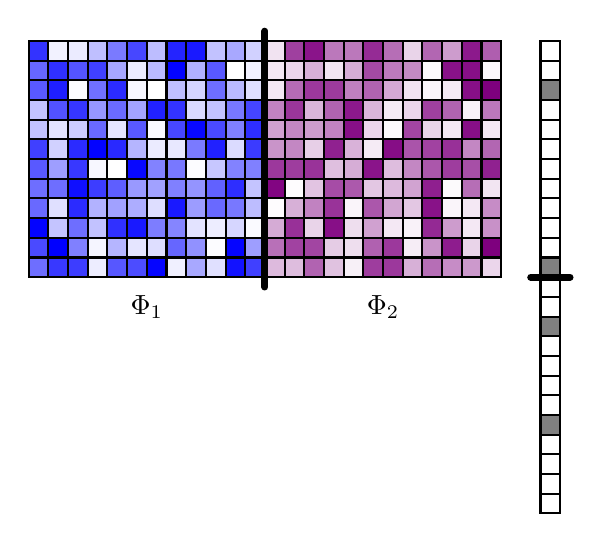
\begin{tikzpicture}
[draw=black, line width=0.75pt,
entry/.style={rectangle, draw, inner sep=0pt, minimum size=2.5mm},
symbol/.style={rectangle, draw, inner sep=0pt, minimum size=2.5mm}]

\node[entry, fill=blue!57] (x0y0) at (0.0,0.0) {};
\node[entry, fill=blue!71] (x0y1) at (0.0,0.25) {};
\node[entry, fill=blue!99] (x0y2) at (0.0,0.5) {};
\node[entry, fill=blue!59] (x0y3) at (0.0,0.75) {};
\node[entry, fill=blue!57] (x0y4) at (0.0,1.0) {};
\node[entry, fill=blue!65] (x0y5) at (0.0,1.25) {};
\node[entry, fill=blue!75] (x0y6) at (0.0,1.5) {};
\node[entry, fill=blue!24] (x0y7) at (0.0,1.75) {};
\node[entry, fill=blue!23] (x0y8) at (0.0,2.0) {};
\node[entry, fill=blue!65] (x0y9) at (0.0,2.25) {};
\node[entry, fill=blue!60] (x0y10) at (0.0,2.5) {};
\node[entry, fill=blue!80] (x0y11) at (0.0,2.75) {};

\node[entry, fill=blue!78] (x1y0) at (0.25,0.0) {};
\node[entry, fill=blue!101] (x1y1) at (0.25,0.25) {};
\node[entry, fill=blue!23] (x1y2) at (0.25,0.5) {};
\node[entry, fill=blue!12] (x1y3) at (0.25,0.75) {};
\node[entry, fill=blue!57] (x1y4) at (0.25,1.0) {};
\node[entry, fill=blue!38] (x1y5) at (0.25,1.25) {};
\node[entry, fill=blue!18] (x1y6) at (0.25,1.5) {};
\node[entry, fill=blue!11] (x1y7) at (0.25,1.75) {};
\node[entry, fill=blue!68] (x1y8) at (0.25,2.0) {};
\node[entry, fill=blue!88] (x1y9) at (0.25,2.25) {};
\node[entry, fill=blue!81] (x1y10) at (0.25,2.5) {};
\node[entry, fill=blue!5] (x1y11) at (0.25,2.75) {};

\node[entry, fill=blue!76] (x2y0) at (0.5,0.0) {};
\node[entry, fill=blue!50] (x2y1) at (0.5,0.25) {};
\node[entry, fill=blue!57] (x2y2) at (0.5,0.5) {};
\node[entry, fill=blue!83] (x2y3) at (0.5,0.75) {};
\node[entry, fill=blue!94] (x2y4) at (0.5,1.0) {};
\node[entry, fill=blue!78] (x2y5) at (0.5,1.25) {};
\node[entry, fill=blue!83] (x2y6) at (0.5,1.5) {};
\node[entry, fill=blue!20] (x2y7) at (0.5,1.75) {};
\node[entry, fill=blue!79] (x2y8) at (0.5,2.0) {};
\node[entry, fill=blue!1] (x2y9) at (0.5,2.25) {};
\node[entry, fill=blue!67] (x2y10) at (0.5,2.5) {};
\node[entry, fill=blue!8] (x2y11) at (0.5,2.75) {};

\node[entry, fill=blue!7] (x3y0) at (0.75,0.0) {};
\node[entry, fill=blue!4] (x3y1) at (0.75,0.25) {};
\node[entry, fill=blue!24] (x3y2) at (0.75,0.5) {};
\node[entry, fill=blue!30] (x3y3) at (0.75,0.75) {};
\node[entry, fill=blue!76] (x3y4) at (0.75,1.0) {};
\node[entry, fill=blue!3] (x3y5) at (0.75,1.25) {};
\node[entry, fill=blue!99] (x3y6) at (0.75,1.5) {};
\node[entry, fill=blue!59] (x3y7) at (0.75,1.75) {};
\node[entry, fill=blue!41] (x3y8) at (0.75,2.0) {};
\node[entry, fill=blue!56] (x3y9) at (0.75,2.25) {};
\node[entry, fill=blue!75] (x3y10) at (0.75,2.5) {};
\node[entry, fill=blue!25] (x3y11) at (0.75,2.75) {};

\node[entry, fill=blue!66] (x4y0) at (1.0,0.0) {};
\node[entry, fill=blue!29] (x4y1) at (1.0,0.25) {};
\node[entry, fill=blue!81] (x4y2) at (1.0,0.5) {};
\node[entry, fill=blue!37] (x4y3) at (1.0,0.75) {};
\node[entry, fill=blue!63] (x4y4) at (1.0,1.0) {};
\node[entry, fill=blue!0] (x4y5) at (1.0,1.25) {};
\node[entry, fill=blue!84] (x4y6) at (1.0,1.5) {};
\node[entry, fill=blue!10] (x4y7) at (1.0,1.75) {};
\node[entry, fill=blue!58] (x4y8) at (1.0,2.0) {};
\node[entry, fill=blue!83] (x4y9) at (1.0,2.25) {};
\node[entry, fill=blue!35] (x4y10) at (1.0,2.5) {};
\node[entry, fill=blue!52] (x4y11) at (1.0,2.75) {};

\node[entry, fill=blue!70] (x5y0) at (1.25,0.0) {};
\node[entry, fill=blue!10] (x5y1) at (1.25,0.25) {};
\node[entry, fill=blue!90] (x5y2) at (1.25,0.5) {};
\node[entry, fill=blue!32] (x5y3) at (1.25,0.75) {};
\node[entry, fill=blue!40] (x5y4) at (1.25,1.0) {};
\node[entry, fill=blue!97] (x5y5) at (1.25,1.25) {};
\node[entry, fill=blue!29] (x5y6) at (1.25,1.5) {};
\node[entry, fill=blue!65] (x5y7) at (1.25,1.75) {};
\node[entry, fill=blue!36] (x5y8) at (1.25,2.0) {};
\node[entry, fill=blue!3] (x5y9) at (1.25,2.25) {};
\node[entry, fill=blue!8] (x5y10) at (1.25,2.5) {};
\node[entry, fill=blue!72] (x5y11) at (1.25,2.75) {};

\node[entry, fill=blue!98] (x6y0) at (1.5,0.0) {};
\node[entry, fill=blue!13] (x6y1) at (1.5,0.25) {};
\node[entry, fill=blue!51] (x6y2) at (1.5,0.5) {};
\node[entry, fill=blue!13] (x6y3) at (1.5,0.75) {};
\node[entry, fill=blue!37] (x6y4) at (1.5,1.0) {};
\node[entry, fill=blue!49] (x6y5) at (1.5,1.25) {};
\node[entry, fill=blue!8] (x6y6) at (1.5,1.5) {};
\node[entry, fill=blue!2] (x6y7) at (1.5,1.75) {};
\node[entry, fill=blue!87] (x6y8) at (1.5,2.0) {};
\node[entry, fill=blue!0] (x6y9) at (1.5,2.25) {};
\node[entry, fill=blue!27] (x6y10) at (1.5,2.5) {};
\node[entry, fill=blue!26] (x6y11) at (1.5,2.75) {};

\node[entry, fill=blue!6] (x7y0) at (1.75,0.0) {};
\node[entry, fill=blue!60] (x7y1) at (1.75,0.25) {};
\node[entry, fill=blue!48] (x7y2) at (1.75,0.5) {};
\node[entry, fill=blue!90] (x7y3) at (1.75,0.75) {};
\node[entry, fill=blue!50] (x7y4) at (1.75,1.0) {};
\node[entry, fill=blue!53] (x7y5) at (1.75,1.25) {};
\node[entry, fill=blue!9] (x7y6) at (1.75,1.5) {};
\node[entry, fill=blue!72] (x7y7) at (1.75,1.75) {};
\node[entry, fill=blue!80] (x7y8) at (1.75,2.0) {};
\node[entry, fill=blue!25] (x7y9) at (1.75,2.25) {};
\node[entry, fill=blue!99] (x7y10) at (1.75,2.5) {};
\node[entry, fill=blue!86] (x7y11) at (1.75,2.75) {};

\node[entry, fill=blue!34] (x8y0) at (2.0,0.0) {};
\node[entry, fill=blue!43] (x8y1) at (2.0,0.25) {};
\node[entry, fill=blue!11] (x8y2) at (2.0,0.5) {};
\node[entry, fill=blue!39] (x8y3) at (2.0,0.75) {};
\node[entry, fill=blue!42] (x8y4) at (2.0,1.0) {};
\node[entry, fill=blue!1] (x8y5) at (2.0,1.25) {};
\node[entry, fill=blue!52] (x8y6) at (2.0,1.5) {};
\node[entry, fill=blue!97] (x8y7) at (2.0,1.75) {};
\node[entry, fill=blue!15] (x8y8) at (2.0,2.0) {};
\node[entry, fill=blue!17] (x8y9) at (2.0,2.25) {};
\node[entry, fill=blue!31] (x8y10) at (2.0,2.5) {};
\node[entry, fill=blue!90] (x8y11) at (2.0,2.75) {};

\node[entry, fill=blue!12] (x9y0) at (2.25,0.0) {};
\node[entry, fill=blue!1] (x9y1) at (2.25,0.25) {};
\node[entry, fill=blue!7] (x9y2) at (2.25,0.5) {};
\node[entry, fill=blue!59] (x9y3) at (2.25,0.75) {};
\node[entry, fill=blue!62] (x9y4) at (2.25,1.0) {};
\node[entry, fill=blue!22] (x9y5) at (2.25,1.25) {};
\node[entry, fill=blue!87] (x9y6) at (2.25,1.5) {};
\node[entry, fill=blue!71] (x9y7) at (2.25,1.75) {};
\node[entry, fill=blue!24] (x9y8) at (2.25,2.0) {};
\node[entry, fill=blue!57] (x9y9) at (2.25,2.25) {};
\node[entry, fill=blue!65] (x9y10) at (2.25,2.5) {};
\node[entry, fill=blue!24] (x9y11) at (2.25,2.75) {};

\node[entry, fill=blue!93] (x10y0) at (2.5,0.0) {};
\node[entry, fill=blue!98] (x10y1) at (2.5,0.25) {};
\node[entry, fill=blue!16] (x10y2) at (2.5,0.5) {};
\node[entry, fill=blue!53] (x10y3) at (2.5,0.75) {};
\node[entry, fill=blue!82] (x10y4) at (2.5,1.0) {};
\node[entry, fill=blue!49] (x10y5) at (2.5,1.25) {};
\node[entry, fill=blue!14] (x10y6) at (2.5,1.5) {};
\node[entry, fill=blue!50] (x10y7) at (2.5,1.75) {};
\node[entry, fill=blue!53] (x10y8) at (2.5,2.0) {};
\node[entry, fill=blue!27] (x10y9) at (2.5,2.25) {};
\node[entry, fill=blue!0] (x10y10) at (2.5,2.5) {};
\node[entry, fill=blue!34] (x10y11) at (2.5,2.75) {};

\node[entry, fill=blue!75] (x11y0) at (2.75,0.0) {};
\node[entry, fill=blue!38] (x11y1) at (2.75,0.25) {};
\node[entry, fill=blue!2] (x11y2) at (2.75,0.5) {};
\node[entry, fill=blue!26] (x11y3) at (2.75,0.75) {};
\node[entry, fill=blue!23] (x11y4) at (2.75,1.0) {};
\node[entry, fill=blue!50] (x11y5) at (2.75,1.25) {};
\node[entry, fill=blue!77] (x11y6) at (2.75,1.5) {};
\node[entry, fill=blue!82] (x11y7) at (2.75,1.75) {};
\node[entry, fill=blue!73] (x11y8) at (2.75,2.0) {};
\node[entry, fill=blue!12] (x11y9) at (2.75,2.25) {};
\node[entry, fill=blue!5] (x11y10) at (2.75,2.5) {};
\node[entry, fill=blue!18] (x11y11) at (2.75,2.75) {};

\node[entry, fill=violet!27] (x12y0) at (3.0,0.0) {};
\node[entry, fill=violet!56] (x12y1) at (3.0,0.25) {};
\node[entry, fill=violet!33] (x12y2) at (3.0,0.5) {};
\node[entry, fill=violet!1] (x12y3) at (3.0,0.75) {};
\node[entry, fill=violet!98] (x12y4) at (3.0,1.0) {};
\node[entry, fill=violet!78] (x12y5) at (3.0,1.25) {};
\node[entry, fill=violet!42] (x12y6) at (3.0,1.5) {};
\node[entry, fill=violet!37] (x12y7) at (3.0,1.75) {};
\node[entry, fill=violet!49] (x12y8) at (3.0,2.0) {};
\node[entry, fill=violet!9] (x12y9) at (3.0,2.25) {};
\node[entry, fill=violet!9] (x12y10) at (3.0,2.5) {};
\node[entry, fill=violet!11] (x12y11) at (3.0,2.75) {};

\node[entry, fill=violet!26] (x13y0) at (3.25,0.0) {};
\node[entry, fill=violet!74] (x13y1) at (3.25,0.25) {};
\node[entry, fill=violet!81] (x13y2) at (3.25,0.5) {};
\node[entry, fill=violet!31] (x13y3) at (3.25,0.75) {};
\node[entry, fill=violet!1] (x13y4) at (3.25,1.0) {};
\node[entry, fill=violet!76] (x13y5) at (3.25,1.25) {};
\node[entry, fill=violet!47] (x13y6) at (3.25,1.5) {};
\node[entry, fill=violet!47] (x13y7) at (3.25,1.75) {};
\node[entry, fill=violet!79] (x13y8) at (3.25,2.0) {};
\node[entry, fill=violet!58] (x13y9) at (3.25,2.25) {};
\node[entry, fill=violet!16] (x13y10) at (3.25,2.5) {};
\node[entry, fill=violet!75] (x13y11) at (3.25,2.75) {};

\node[entry, fill=violet!61] (x14y0) at (3.5,0.0) {};
\node[entry, fill=violet!73] (x14y1) at (3.5,0.25) {};
\node[entry, fill=violet!17] (x14y2) at (3.5,0.5) {};
\node[entry, fill=violet!49] (x14y3) at (3.5,0.75) {};
\node[entry, fill=violet!23] (x14y4) at (3.5,1.0) {};
\node[entry, fill=violet!80] (x14y5) at (3.5,1.25) {};
\node[entry, fill=violet!19] (x14y6) at (3.5,1.5) {};
\node[entry, fill=violet!39] (x14y7) at (3.5,1.75) {};
\node[entry, fill=violet!29] (x14y8) at (3.5,2.0) {};
\node[entry, fill=violet!78] (x14y9) at (3.5,2.25) {};
\node[entry, fill=violet!31] (x14y10) at (3.5,2.5) {};
\node[entry, fill=violet!92] (x14y11) at (3.5,2.75) {};

\node[entry, fill=violet!24] (x15y0) at (3.75,0.0) {};
\node[entry, fill=violet!20] (x15y1) at (3.75,0.25) {};
\node[entry, fill=violet!94] (x15y2) at (3.75,0.5) {};
\node[entry, fill=violet!80] (x15y3) at (3.75,0.75) {};
\node[entry, fill=violet!70] (x15y4) at (3.75,1.0) {};
\node[entry, fill=violet!25] (x15y5) at (3.75,1.25) {};
\node[entry, fill=violet!87] (x15y6) at (3.75,1.5) {};
\node[entry, fill=violet!49] (x15y7) at (3.75,1.75) {};
\node[entry, fill=violet!61] (x15y8) at (3.75,2.0) {};
\node[entry, fill=violet!77] (x15y9) at (3.75,2.25) {};
\node[entry, fill=violet!10] (x15y10) at (3.75,2.5) {};
\node[entry, fill=violet!53] (x15y11) at (3.75,2.75) {};

\node[entry, fill=violet!6] (x16y0) at (4.0,0.0) {};
\node[entry, fill=violet!13] (x16y1) at (4.0,0.25) {};
\node[entry, fill=violet!13] (x16y2) at (4.0,0.5) {};
\node[entry, fill=violet!4] (x16y3) at (4.0,0.75) {};
\node[entry, fill=violet!65] (x16y4) at (4.0,1.0) {};
\node[entry, fill=violet!32] (x16y5) at (4.0,1.25) {};
\node[entry, fill=violet!30] (x16y6) at (4.0,1.5) {};
\node[entry, fill=violet!94] (x16y7) at (4.0,1.75) {};
\node[entry, fill=violet!90] (x16y8) at (4.0,2.0) {};
\node[entry, fill=violet!50] (x16y9) at (4.0,2.25) {};
\node[entry, fill=violet!32] (x16y10) at (4.0,2.5) {};
\node[entry, fill=violet!53] (x16y11) at (4.0,2.75) {};

\node[entry, fill=violet!76] (x17y0) at (4.25,0.0) {};
\node[entry, fill=violet!62] (x17y1) at (4.25,0.25) {};
\node[entry, fill=violet!37] (x17y2) at (4.25,0.5) {};
\node[entry, fill=violet!66] (x17y3) at (4.25,0.75) {};
\node[entry, fill=violet!22] (x17y4) at (4.25,1.0) {};
\node[entry, fill=violet!92] (x17y5) at (4.25,1.25) {};
\node[entry, fill=violet!8] (x17y6) at (4.25,1.5) {};
\node[entry, fill=violet!16] (x17y7) at (4.25,1.75) {};
\node[entry, fill=violet!29] (x17y8) at (4.25,2.0) {};
\node[entry, fill=violet!61] (x17y9) at (4.25,2.25) {};
\node[entry, fill=violet!71] (x17y10) at (4.25,2.5) {};
\node[entry, fill=violet!83] (x17y11) at (4.25,2.75) {};

\node[entry, fill=violet!78] (x18y0) at (4.5,0.0) {};
\node[entry, fill=violet!78] (x18y1) at (4.5,0.25) {};
\node[entry, fill=violet!9] (x18y2) at (4.5,0.5) {};
\node[entry, fill=violet!35] (x18y3) at (4.5,0.75) {};
\node[entry, fill=violet!27] (x18y4) at (4.5,1.0) {};
\node[entry, fill=violet!26] (x18y5) at (4.5,1.25) {};
\node[entry, fill=violet!95] (x18y6) at (4.5,1.5) {};
\node[entry, fill=violet!2] (x18y7) at (4.5,1.75) {};
\node[entry, fill=violet!8] (x18y8) at (4.5,2.0) {};
\node[entry, fill=violet!34] (x18y9) at (4.5,2.25) {};
\node[entry, fill=violet!52] (x18y10) at (4.5,2.5) {};
\node[entry, fill=violet!57] (x18y11) at (4.5,2.75) {};

\node[entry, fill=violet!31] (x19y0) at (4.75,0.0) {};
\node[entry, fill=violet!7] (x19y1) at (4.75,0.25) {};
\node[entry, fill=violet!5] (x19y2) at (4.75,0.5) {};
\node[entry, fill=violet!22] (x19y3) at (4.75,0.75) {};
\node[entry, fill=violet!36] (x19y4) at (4.75,1.0) {};
\node[entry, fill=violet!47] (x19y5) at (4.75,1.25) {};
\node[entry, fill=violet!67] (x19y6) at (4.75,1.5) {};
\node[entry, fill=violet!73] (x19y7) at (4.75,1.75) {};
\node[entry, fill=violet!16] (x19y8) at (4.75,2.0) {};
\node[entry, fill=violet!11] (x19y9) at (4.75,2.25) {};
\node[entry, fill=violet!46] (x19y10) at (4.75,2.5) {};
\node[entry, fill=violet!17] (x19y11) at (4.75,2.75) {};

\node[entry, fill=violet!57] (x20y0) at (5.0,0.0) {};
\node[entry, fill=violet!42] (x20y1) at (5.0,0.25) {};
\node[entry, fill=violet!84] (x20y2) at (5.0,0.5) {};
\node[entry, fill=violet!93] (x20y3) at (5.0,0.75) {};
\node[entry, fill=violet!88] (x20y4) at (5.0,1.0) {};
\node[entry, fill=violet!66] (x20y5) at (5.0,1.25) {};
\node[entry, fill=violet!74] (x20y6) at (5.0,1.5) {};
\node[entry, fill=violet!17] (x20y7) at (5.0,1.75) {};
\node[entry, fill=violet!75] (x20y8) at (5.0,2.0) {};
\node[entry, fill=violet!4] (x20y9) at (5.0,2.25) {};
\node[entry, fill=violet!2] (x20y10) at (5.0,2.5) {};
\node[entry, fill=violet!60] (x20y11) at (5.0,2.75) {};

\node[entry, fill=violet!45] (x21y0) at (5.25,0.0) {};
\node[entry, fill=violet!89] (x21y1) at (5.25,0.25) {};
\node[entry, fill=violet!39] (x21y2) at (5.25,0.5) {};
\node[entry, fill=violet!4] (x21y3) at (5.25,0.75) {};
\node[entry, fill=violet!2] (x21y4) at (5.25,1.0) {};
\node[entry, fill=violet!76] (x21y5) at (5.25,1.25) {};
\node[entry, fill=violet!81] (x21y6) at (5.25,1.5) {};
\node[entry, fill=violet!9] (x21y7) at (5.25,1.75) {};
\node[entry, fill=violet!61] (x21y8) at (5.25,2.0) {};
\node[entry, fill=violet!8] (x21y9) at (5.25,2.25) {};
\node[entry, fill=violet!93] (x21y10) at (5.25,2.5) {};
\node[entry, fill=violet!39] (x21y11) at (5.25,2.75) {};

\node[entry, fill=violet!40] (x22y0) at (5.5,0.0) {};
\node[entry, fill=violet!17] (x22y1) at (5.5,0.25) {};
\node[entry, fill=violet!9] (x22y2) at (5.5,0.5) {};
\node[entry, fill=violet!9] (x22y3) at (5.5,0.75) {};
\node[entry, fill=violet!57] (x22y4) at (5.5,1.0) {};
\node[entry, fill=violet!69] (x22y5) at (5.5,1.25) {};
\node[entry, fill=violet!47] (x22y6) at (5.5,1.5) {};
\node[entry, fill=violet!94] (x22y7) at (5.5,1.75) {};
\node[entry, fill=violet!5] (x22y8) at (5.5,2.0) {};
\node[entry, fill=violet!94] (x22y9) at (5.5,2.25) {};
\node[entry, fill=violet!94] (x22y10) at (5.5,2.5) {};
\node[entry, fill=violet!90] (x22y11) at (5.5,2.75) {};

\node[entry, fill=violet!16] (x23y0) at (5.75,0.0) {};
\node[entry, fill=violet!101] (x23y1) at (5.75,0.25) {};
\node[entry, fill=violet!43] (x23y2) at (5.75,0.5) {};
\node[entry, fill=violet!45] (x23y3) at (5.75,0.75) {};
\node[entry, fill=violet!10] (x23y4) at (5.75,1.0) {};
\node[entry, fill=violet!87] (x23y5) at (5.75,1.25) {};
\node[entry, fill=violet!60] (x23y6) at (5.75,1.5) {};
\node[entry, fill=violet!9] (x23y7) at (5.75,1.75) {};
\node[entry, fill=violet!53] (x23y8) at (5.75,2.0) {};
\node[entry, fill=violet!101] (x23y9) at (5.75,2.25) {};
\node[entry, fill=violet!3] (x23y10) at (5.75,2.5) {};
\node[entry, fill=violet!63] (x23y11) at (5.75,2.75) {};

\node[symbol] (s01) at (6.5,-3.00) {};
\node[symbol] (s02) at (6.5,-2.75) {};
\node[symbol] (s03) at (6.5,-2.50) {};
\node[symbol] (s04) at (6.5,-2.25) {};
\node[symbol,fill=gray] (s05) at (6.5,-2.00) {};
\node[symbol] (s06) at (6.5,-1.75) {};
\node[symbol] (s07) at (6.5,-1.50) {};
\node[symbol] (s08) at (6.5,-1.25) {};
\node[symbol] (s09) at (6.5,-1.00) {};
\node[symbol,fill=gray] (s10) at (6.5,-0.75) {};
\node[symbol] (s11) at (6.5,-0.50) {};
\node[symbol] (s12) at (6.5,-0.25) {};
\node[symbol,fill=gray] (s13) at (6.5,0) {};
\node[symbol] (s14) at (6.5,0.25) {};
\node[symbol] (s15) at (6.5,0.50) {};
\node[symbol] (s16) at (6.5,0.75) {};
\node[symbol] (s17) at (6.5,1.00) {};
\node[symbol] (s18) at (6.5,1.25) {};
\node[symbol] (s19) at (6.5,1.50) {};
\node[symbol] (s20) at (6.5,1.75) {};
\node[symbol] (s21) at (6.5,2.00) {};
\node[symbol,fill=gray] (s22) at (6.5,2.25) {};
\node[symbol] (s23) at (6.5,2.50) {};
\node[symbol] (s24) at (6.5,2.75) {};

\draw[line width=2.5pt,line cap=round] (2.875,-0.25) to (2.875,3);
\draw[line width=2.5pt,line cap=round] (6.25,-0.125) to (6.75,-0.125);

\node at (1.375,-0.5) {$\boldsymbol{\Phi}_1$};
\node at (4.375,-0.5) {$\boldsymbol{\Phi}_2$};

\end{tikzpicture}
}
\end{columns}
% % % % %
\vfill
% % % % %
\begin{alertblock}{Drawbacks}
  \begin{itemize}
  \item Low complexity joint multi-user decoders are not available
  \item Devices may collide within codebook selection
  \end{itemize}
\end{alertblock}
\end{frame}

% % % % % % % % % % % % % % % % % % % %

\begin{frame}
\frametitle{Data Fragmentation}
% % % % %
\begin{center}
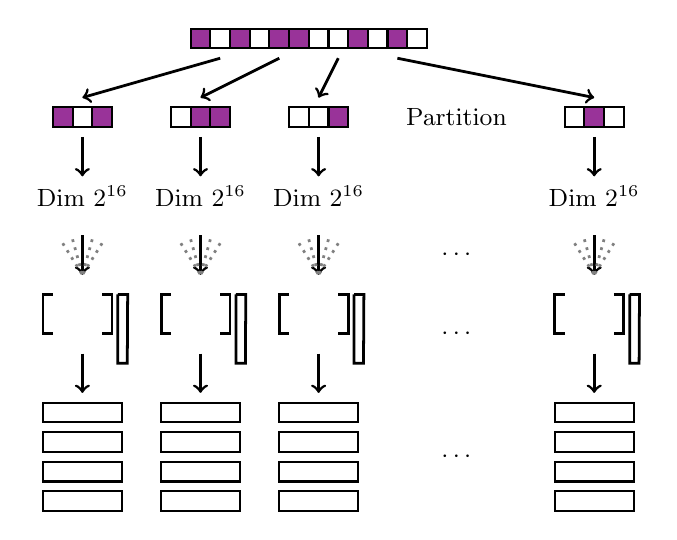
\begin{tikzpicture}
[font=\small, draw=black, line width=0.75pt,
sub0/.style={rectangle, draw, inner sep=0pt, minimum width=10mm, minimum height=2.5mm},
parity/.style={rectangle, draw, fill=cyan, inner sep=0pt, minimum size=2.5mm},
bit0/.style={rectangle, draw, inner sep=0pt, minimum size=2.5mm},
bit1/.style={rectangle, draw, fill=violet!80, inner sep=0pt, minimum size=2.5mm}]

\node[bit1] (bit0) at (0.50,8.25) {};
\node[bit0] (bit1) at (0.75,8.25) {};
\node[bit1] (bit2) at (1.00,8.25) {};
\node[bit0] (bit3) at (1.25,8.25) {};
\node[bit1] (bit4) at (1.50,8.25) {};
\node[bit1] (bit5) at (1.75,8.25) {};
\node[bit0] (bit6) at (2.00,8.25) {};
\node[bit0] (bit7) at (2.25,8.25) {};
\node[bit1] (bit8) at (2.50,8.25) {};
\node[bit0] (bit9) at (2.75,8.25) {};
\node[bit1] (bit10) at (3.00,8.25) {};
\node[bit0] (bit11) at (3.25,8.25) {};

\draw[->, line width=1pt]  (0.75,8.00) -- (-1.00,7.50);
\draw[->, line width=1pt]  (1.50,8.00) -- (0.50,7.50);
\draw[->, line width=1pt]  (2.25,8.00) -- (2.00,7.50);
\draw[->, line width=1pt]  (3.00,8.00) -- (5.50,7.50);
\node (partition) at (3.75,7.25) {Partition};

\node[bit1] (s00) at (-1.25,7.25) {};
\node[bit0] (s01) at (-1.00,7.25) {};
\node[bit1] (s02) at (-0.75,7.25) {};

\node[bit0] (s03) at (0.25,7.25) {};
\node[bit1] (s04) at (0.50,7.25) {};
\node[bit1] (s05) at (0.75,7.25) {};

\node[bit0] (s06) at (1.75,7.25) {};
\node[bit0] (s07) at (2.00,7.25) {};
\node[bit1] (s08) at (2.25,7.25) {};

\node[bit0] (s09) at (5.25,7.25) {};
\node[bit1] (s10) at (5.50,7.25) {};
\node[bit0] (s11) at (5.75,7.25) {};

\draw[->, line width=1pt]  (-1.00,7) -- (-1.00,6.5);
\draw[->, line width=1pt]  (0.50,7) -- (0.50,6.5);
\draw[->, line width=1pt]  (2.00,7) -- (2.00,6.5);
\draw[->, line width=1pt]  (5.50,7) -- (5.50,6.5);

\node (cs1) at (-1.00,6.25) {Dim~$2^{16}$};
\node (cs2) at (0.50,6.25) {Dim~$2^{16}$};
\node (cs3) at (2.00,6.25) {Dim~$2^{16}$};
\node (cs4) at (5.50,6.25) {Dim~$2^{16}$};

\foreach \v in {-1.00,0.50,2.00,5.50} {
  \draw[->, line width=1pt]  (\v,4.25) -- (\v,3.75);
  \draw[->, line width=1pt]  (\v,5.75) -- (\v,5.25);
  \draw[dotted, line width=1pt, draw=gray]  (\v-0.25,5.65) -- (\v,5.25);
  \draw[dotted, line width=1pt, draw=gray]  (\v-0.125,5.7) -- (\v,5.25);
  \draw[dotted, line width=1pt, draw=gray]  (\v+0.125,5.7) -- (\v,5.25);
  \draw[dotted, line width=1pt, draw=gray]  (\v+0.25,5.65) -- (\v,5.25);
}

\node (dots1) at (3.75,5.5) {$\cdots$};

\foreach \v in {-1.00,0.50,2.00,5.50} {
  \draw[line width=1pt] (\v-0.375,5) -- (\v-0.5,5) -- (\v-0.5,4.5) -- (\v-0.375,4.5);
  \draw[line width=1pt] (\v+0.25,5) -- (\v+0.375,5) -- (\v+0.375,4.5) -- (\v+0.25,4.5);
  \draw[line width=1pt] (\v+0.45,5) -- (\v+0.45,4.125) -- (\v+0.57,4.125) -- (\v+0.575,5) -- (\v+0.45,5);
}

\node (dots2) at (3.75,4.5) {$\cdots$};
\node (dots3) at (3.75,2.9375) {$\cdots$};

\foreach \c in {3.50, 3.125, 2.75, 2.375} {
  \node[sub0] (subcs0\c) at (-1.00,\c) {};
  \node[sub0] (subcs2\c) at (0.50,\c) {};
  \node[sub0] (subcs3\c) at (2.00,\c) {};
  \node[sub0] (subcsz\c) at (5.50,\c) {};
}

%\node (list1) at (-1.00,1.875) {List~1};
%\node (list2) at (0.50,1.875) {List~2};
%\node (list3) at (2.00,1.875) {List~3};
%\node (list4) at (5.50,1.875) {List~$L$};
\end{tikzpicture}

\end{center}
% % % % %
\begin{alertblock}{Drawbacks}
  \begin{itemize}
  \item Unordered lists of fragments
  \item Need to perform disambiguation
  \end{itemize}
\end{alertblock}
\end{frame}

% % % % % % % % % % % % % % % % % % % %

\begin{frame} \frametitle{Drastic Reduction in Matrix Width}
\begin{center} 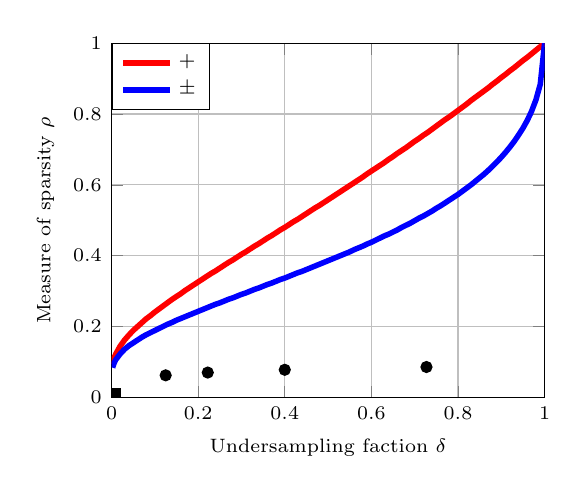
\begin{tikzpicture}

\begin{axis}[%
font=\scriptsize,
width=5.5cm,
height=4.5cm,
scale only axis,
xmin=0,
xmax=1,
xlabel={Undersampling faction $\delta$},
xmajorgrids,
ymin=0,
ymax=1,
ylabel={Measure of sparsity $\rho$},
%ylabel near ticks,
ymajorgrids,
legend style={at={(0,1)},anchor=north west,legend cell align=left,
/tikz/column 2/.style={column sep=3pt}}
]

\addplot [color=red,solid,line width=2.0pt]
  coordinates {
(0.0025,0.094) (0.005,0.107) (0.0075,0.116)
(0.01,0.123) (0.02,0.145) (0.03,0.162) (0.04,0.176) (0.05,0.189) (0.06,0.2) (0.07,0.211) (0.08,0.222) (0.09,0.231) (0.1,0.241) (0.11,0.25) (0.12,0.259) (0.13,0.268) (0.14,0.277) (0.15,0.285) (0.16,0.293) (0.17,0.302) (0.18,0.31) (0.19,0.318) (0.2,0.326) (0.21,0.334) (0.22,0.342) (0.23,0.35) (0.24,0.357) (0.25,0.365) (0.26,0.373) (0.27,0.381) (0.28,0.388) (0.29,0.396) (0.3,0.404) (0.31,0.411) (0.32,0.419) (0.33,0.427) (0.34,0.434) (0.35,0.442) (0.36,0.45) (0.37,0.457) (0.38,0.465) (0.39,0.473) (0.4,0.48) (0.41,0.488) (0.42,0.496) (0.43,0.503) (0.44,0.511) (0.45,0.519) (0.46,0.527) (0.47,0.535) (0.48,0.542) (0.49,0.55) (0.5,0.558) (0.51,0.566) (0.52,0.574) (0.53,0.582) (0.54,0.59) (0.55,0.598) (0.56,0.606) (0.57,0.614) (0.58,0.622) (0.59,0.631) (0.6,0.639) (0.61,0.647) (0.62,0.655) (0.63,0.663) (0.64,0.672) (0.65,0.68) (0.66,0.689) (0.67,0.697) (0.68,0.705) (0.69,0.714) (0.7,0.723) (0.71,0.731) (0.72,0.74) (0.73,0.748) (0.74,0.757) (0.75,0.766) (0.76,0.775) (0.77,0.784) (0.78,0.792) (0.79,0.801) (0.8,0.81) (0.81,0.819) (0.82,0.828) (0.83,0.838) (0.84,0.847) (0.85,0.856) (0.86,0.865) (0.87,0.874) (0.88,0.884) (0.89,0.893) (0.9,0.903) (0.91,0.912) (0.92,0.922) (0.93,0.931) (0.94,0.941) (0.95,0.951) (0.96,0.96) (0.97,0.97) (0.98,0.98) (0.99,0.99) (1,1)
};
\addlegendentry{$+$};

\addplot [color=blue,solid,line width=2.0pt]
  coordinates {
(0.0025,0.084) (0.005,0.094) (0.0075,0.101)
(0.01,0.107) (0.02,0.123) (0.03,0.136) (0.04,0.146) (0.05,0.154) (0.06,0.162) (0.07,0.17) (0.08,0.177) (0.09,0.183) (0.1,0.189) (0.11,0.195) (0.12,0.201) (0.13,0.207) (0.14,0.212) (0.15,0.218) (0.16,0.223) (0.17,0.228) (0.18,0.233) (0.19,0.238) (0.2,0.243) (0.21,0.248) (0.22,0.253) (0.23,0.258) (0.24,0.263) (0.25,0.267) (0.26,0.272) (0.27,0.277) (0.28,0.281) (0.29,0.286) (0.3,0.291) (0.31,0.295) (0.32,0.3) (0.33,0.305) (0.34,0.309) (0.35,0.314) (0.36,0.319) (0.37,0.323) (0.38,0.328) (0.39,0.333) (0.4,0.337) (0.41,0.342) (0.42,0.347) (0.43,0.352) (0.44,0.356) (0.45,0.361) (0.46,0.366) (0.47,0.371) (0.48,0.376) (0.49,0.381) (0.5,0.386) (0.51,0.391) (0.52,0.396) (0.53,0.401) (0.54,0.406) (0.55,0.411) (0.56,0.417) (0.57,0.422) (0.58,0.427) (0.59,0.433) (0.6,0.438) (0.61,0.444) (0.62,0.45) (0.63,0.456) (0.64,0.461) (0.65,0.467) (0.66,0.473) (0.67,0.48) (0.68,0.486) (0.69,0.492) (0.7,0.499) (0.71,0.506) (0.72,0.512) (0.73,0.519) (0.74,0.526) (0.75,0.534) (0.76,0.541) (0.77,0.549) (0.78,0.557) (0.79,0.565) (0.8,0.573) (0.81,0.582) (0.82,0.591) (0.83,0.6) (0.84,0.61) (0.85,0.62) (0.86,0.63) (0.87,0.641) (0.88,0.653) (0.89,0.665) (0.9,0.678) (0.91,0.692) (0.92,0.707) (0.93,0.723) (0.94,0.741) (0.95,0.76) (0.96,0.782) (0.97,0.808) (0.98,0.84) (0.99,0.884) (1,1)
};
\addlegendentry{$\pm$};

%\node at (axis cs: 0.2, 0.65) {Failure Region};
%\node at (axis cs: 0.685, 0.25) {Exact Reconstruction};

\filldraw [fill=black] (axis cs:0,0) rectangle (axis cs:0.02,0.025);

\filldraw (axis cs: 0.125, 0.0625) circle (2pt);
\filldraw (axis cs: 0.2222,0.0703125) circle (2pt);
\filldraw (axis cs: 0.4, 0.078125) circle (2pt);
\filldraw (axis cs: 0.7272,0.0859375) circle (2pt);

%\filldraw[color=darkgray] (axis cs: 0.000001, 0.0625) circle (1.5pt);
%\filldraw[color=darkgray] (axis cs: 0.000006, 0.0703125) circle (1.5pt);
%\filldraw[color=darkgray] (axis cs: 0.00004, 0.078125) circle (1.5pt);
%\filldraw[color=darkgray] (axis cs: 0.00018, 0.0859375) circle (1.5pt);
%\filldraw[color=darkgray] (axis cs: 0.00065, 0.09375) circle (1.5pt);
%\filldraw[color=darkgray] (axis cs: 0.00240, 0.1015625) circle (1.5pt);
%\filldraw[color=darkgray] (axis cs: 0.00446, 0.109375) circle (1.5pt);
%\filldraw[color=darkgray] (axis cs: 0.00833, 0.1171875) circle (1.5pt);
%\filldraw[color=darkgray] (axis cs: 0.03125, 0.125) circle (1.5pt);
%\filldraw[color=darkgray] (axis cs: 0.055555, 0.140625) circle (1.5pt);
%\filldraw[color=darkgray] (axis cs: 0.2, 0.15625) circle (1.5pt);
\end{axis}

\end{tikzpicture}
 \end{center}
% % % % %
\begin{columns}
\column{0.48\textwidth}
\begin{itemize}
\item Undersampling fraction \[ \delta = \frac{32,768}{L \cdot 2^{\lceil 128/L \rceil}} \]
\end{itemize}
\column{0.48\textwidth}
\begin{itemize}
\item Measure of sparsity \[ \rho = \frac{L \cdot 256}{32,768} = \frac{L}{2^7} \]
\end{itemize}
\end{columns}
% % % % %
\end{frame}

% % % % % % % % % % % % % % % % % % % %

\begin{frame}
\frametitle{Section Summary}
% % % % %
\begin{columns}
\column{0.54\textwidth}
\structure{\large Problem formulation}
  \begin{itemize}
  \item Noisy compressed sensing
  \begin{equation*}
  \yv = \boldsymbol{\Phi} \sv + \zv
  \end{equation*}
  \item URA is noisy support recovery
  \item Full control over $\boldsymbol{\Phi}$
  \item Width of sensing matrix is huge
  \item Uncoordinated access produces stochastic binning
  \end{itemize}
\column{0.44\textwidth}
  \hspace{-1cm} \scalebox{0.75}{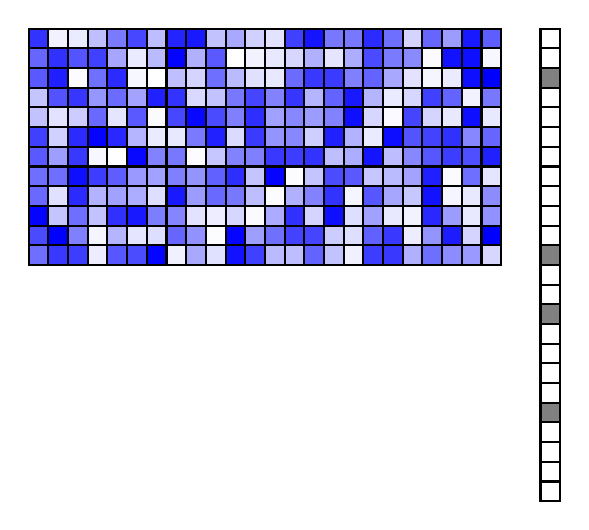
\begin{tikzpicture}
[draw=black, line width=0.75pt,
entry/.style={rectangle, draw, inner sep=0pt, minimum size=2.5mm},
symbol/.style={rectangle, draw, inner sep=0pt, minimum size=2.5mm}]

\node[entry, fill=blue!57] (x0y0) at (0.0,0.0) {};
\node[entry, fill=blue!71] (x0y1) at (0.0,0.25) {};
\node[entry, fill=blue!99] (x0y2) at (0.0,0.5) {};
\node[entry, fill=blue!59] (x0y3) at (0.0,0.75) {};
\node[entry, fill=blue!57] (x0y4) at (0.0,1.0) {};
\node[entry, fill=blue!65] (x0y5) at (0.0,1.25) {};
\node[entry, fill=blue!75] (x0y6) at (0.0,1.5) {};
\node[entry, fill=blue!24] (x0y7) at (0.0,1.75) {};
\node[entry, fill=blue!23] (x0y8) at (0.0,2.0) {};
\node[entry, fill=blue!65] (x0y9) at (0.0,2.25) {};
\node[entry, fill=blue!60] (x0y10) at (0.0,2.5) {};
\node[entry, fill=blue!80] (x0y11) at (0.0,2.75) {};

\node[entry, fill=blue!78] (x1y0) at (0.25,0.0) {};
\node[entry, fill=blue!101] (x1y1) at (0.25,0.25) {};
\node[entry, fill=blue!23] (x1y2) at (0.25,0.5) {};
\node[entry, fill=blue!12] (x1y3) at (0.25,0.75) {};
\node[entry, fill=blue!57] (x1y4) at (0.25,1.0) {};
\node[entry, fill=blue!38] (x1y5) at (0.25,1.25) {};
\node[entry, fill=blue!18] (x1y6) at (0.25,1.5) {};
\node[entry, fill=blue!11] (x1y7) at (0.25,1.75) {};
\node[entry, fill=blue!68] (x1y8) at (0.25,2.0) {};
\node[entry, fill=blue!88] (x1y9) at (0.25,2.25) {};
\node[entry, fill=blue!81] (x1y10) at (0.25,2.5) {};
\node[entry, fill=blue!5] (x1y11) at (0.25,2.75) {};

\node[entry, fill=blue!76] (x2y0) at (0.5,0.0) {};
\node[entry, fill=blue!50] (x2y1) at (0.5,0.25) {};
\node[entry, fill=blue!57] (x2y2) at (0.5,0.5) {};
\node[entry, fill=blue!83] (x2y3) at (0.5,0.75) {};
\node[entry, fill=blue!94] (x2y4) at (0.5,1.0) {};
\node[entry, fill=blue!78] (x2y5) at (0.5,1.25) {};
\node[entry, fill=blue!83] (x2y6) at (0.5,1.5) {};
\node[entry, fill=blue!20] (x2y7) at (0.5,1.75) {};
\node[entry, fill=blue!79] (x2y8) at (0.5,2.0) {};
\node[entry, fill=blue!1] (x2y9) at (0.5,2.25) {};
\node[entry, fill=blue!67] (x2y10) at (0.5,2.5) {};
\node[entry, fill=blue!8] (x2y11) at (0.5,2.75) {};

\node[entry, fill=blue!7] (x3y0) at (0.75,0.0) {};
\node[entry, fill=blue!4] (x3y1) at (0.75,0.25) {};
\node[entry, fill=blue!24] (x3y2) at (0.75,0.5) {};
\node[entry, fill=blue!30] (x3y3) at (0.75,0.75) {};
\node[entry, fill=blue!76] (x3y4) at (0.75,1.0) {};
\node[entry, fill=blue!3] (x3y5) at (0.75,1.25) {};
\node[entry, fill=blue!99] (x3y6) at (0.75,1.5) {};
\node[entry, fill=blue!59] (x3y7) at (0.75,1.75) {};
\node[entry, fill=blue!41] (x3y8) at (0.75,2.0) {};
\node[entry, fill=blue!56] (x3y9) at (0.75,2.25) {};
\node[entry, fill=blue!75] (x3y10) at (0.75,2.5) {};
\node[entry, fill=blue!25] (x3y11) at (0.75,2.75) {};

\node[entry, fill=blue!66] (x4y0) at (1.0,0.0) {};
\node[entry, fill=blue!29] (x4y1) at (1.0,0.25) {};
\node[entry, fill=blue!81] (x4y2) at (1.0,0.5) {};
\node[entry, fill=blue!37] (x4y3) at (1.0,0.75) {};
\node[entry, fill=blue!63] (x4y4) at (1.0,1.0) {};
\node[entry, fill=blue!0] (x4y5) at (1.0,1.25) {};
\node[entry, fill=blue!84] (x4y6) at (1.0,1.5) {};
\node[entry, fill=blue!10] (x4y7) at (1.0,1.75) {};
\node[entry, fill=blue!58] (x4y8) at (1.0,2.0) {};
\node[entry, fill=blue!83] (x4y9) at (1.0,2.25) {};
\node[entry, fill=blue!35] (x4y10) at (1.0,2.5) {};
\node[entry, fill=blue!52] (x4y11) at (1.0,2.75) {};

\node[entry, fill=blue!70] (x5y0) at (1.25,0.0) {};
\node[entry, fill=blue!10] (x5y1) at (1.25,0.25) {};
\node[entry, fill=blue!90] (x5y2) at (1.25,0.5) {};
\node[entry, fill=blue!32] (x5y3) at (1.25,0.75) {};
\node[entry, fill=blue!40] (x5y4) at (1.25,1.0) {};
\node[entry, fill=blue!97] (x5y5) at (1.25,1.25) {};
\node[entry, fill=blue!29] (x5y6) at (1.25,1.5) {};
\node[entry, fill=blue!65] (x5y7) at (1.25,1.75) {};
\node[entry, fill=blue!36] (x5y8) at (1.25,2.0) {};
\node[entry, fill=blue!3] (x5y9) at (1.25,2.25) {};
\node[entry, fill=blue!8] (x5y10) at (1.25,2.5) {};
\node[entry, fill=blue!72] (x5y11) at (1.25,2.75) {};

\node[entry, fill=blue!98] (x6y0) at (1.5,0.0) {};
\node[entry, fill=blue!13] (x6y1) at (1.5,0.25) {};
\node[entry, fill=blue!51] (x6y2) at (1.5,0.5) {};
\node[entry, fill=blue!13] (x6y3) at (1.5,0.75) {};
\node[entry, fill=blue!37] (x6y4) at (1.5,1.0) {};
\node[entry, fill=blue!49] (x6y5) at (1.5,1.25) {};
\node[entry, fill=blue!8] (x6y6) at (1.5,1.5) {};
\node[entry, fill=blue!2] (x6y7) at (1.5,1.75) {};
\node[entry, fill=blue!87] (x6y8) at (1.5,2.0) {};
\node[entry, fill=blue!0] (x6y9) at (1.5,2.25) {};
\node[entry, fill=blue!27] (x6y10) at (1.5,2.5) {};
\node[entry, fill=blue!26] (x6y11) at (1.5,2.75) {};

\node[entry, fill=blue!6] (x7y0) at (1.75,0.0) {};
\node[entry, fill=blue!60] (x7y1) at (1.75,0.25) {};
\node[entry, fill=blue!48] (x7y2) at (1.75,0.5) {};
\node[entry, fill=blue!90] (x7y3) at (1.75,0.75) {};
\node[entry, fill=blue!50] (x7y4) at (1.75,1.0) {};
\node[entry, fill=blue!53] (x7y5) at (1.75,1.25) {};
\node[entry, fill=blue!9] (x7y6) at (1.75,1.5) {};
\node[entry, fill=blue!72] (x7y7) at (1.75,1.75) {};
\node[entry, fill=blue!80] (x7y8) at (1.75,2.0) {};
\node[entry, fill=blue!25] (x7y9) at (1.75,2.25) {};
\node[entry, fill=blue!99] (x7y10) at (1.75,2.5) {};
\node[entry, fill=blue!86] (x7y11) at (1.75,2.75) {};

\node[entry, fill=blue!34] (x8y0) at (2.0,0.0) {};
\node[entry, fill=blue!43] (x8y1) at (2.0,0.25) {};
\node[entry, fill=blue!11] (x8y2) at (2.0,0.5) {};
\node[entry, fill=blue!39] (x8y3) at (2.0,0.75) {};
\node[entry, fill=blue!42] (x8y4) at (2.0,1.0) {};
\node[entry, fill=blue!1] (x8y5) at (2.0,1.25) {};
\node[entry, fill=blue!52] (x8y6) at (2.0,1.5) {};
\node[entry, fill=blue!97] (x8y7) at (2.0,1.75) {};
\node[entry, fill=blue!15] (x8y8) at (2.0,2.0) {};
\node[entry, fill=blue!17] (x8y9) at (2.0,2.25) {};
\node[entry, fill=blue!31] (x8y10) at (2.0,2.5) {};
\node[entry, fill=blue!90] (x8y11) at (2.0,2.75) {};

\node[entry, fill=blue!12] (x9y0) at (2.25,0.0) {};
\node[entry, fill=blue!1] (x9y1) at (2.25,0.25) {};
\node[entry, fill=blue!7] (x9y2) at (2.25,0.5) {};
\node[entry, fill=blue!59] (x9y3) at (2.25,0.75) {};
\node[entry, fill=blue!62] (x9y4) at (2.25,1.0) {};
\node[entry, fill=blue!22] (x9y5) at (2.25,1.25) {};
\node[entry, fill=blue!87] (x9y6) at (2.25,1.5) {};
\node[entry, fill=blue!71] (x9y7) at (2.25,1.75) {};
\node[entry, fill=blue!24] (x9y8) at (2.25,2.0) {};
\node[entry, fill=blue!57] (x9y9) at (2.25,2.25) {};
\node[entry, fill=blue!65] (x9y10) at (2.25,2.5) {};
\node[entry, fill=blue!24] (x9y11) at (2.25,2.75) {};

\node[entry, fill=blue!93] (x10y0) at (2.5,0.0) {};
\node[entry, fill=blue!98] (x10y1) at (2.5,0.25) {};
\node[entry, fill=blue!16] (x10y2) at (2.5,0.5) {};
\node[entry, fill=blue!53] (x10y3) at (2.5,0.75) {};
\node[entry, fill=blue!82] (x10y4) at (2.5,1.0) {};
\node[entry, fill=blue!49] (x10y5) at (2.5,1.25) {};
\node[entry, fill=blue!14] (x10y6) at (2.5,1.5) {};
\node[entry, fill=blue!50] (x10y7) at (2.5,1.75) {};
\node[entry, fill=blue!53] (x10y8) at (2.5,2.0) {};
\node[entry, fill=blue!27] (x10y9) at (2.5,2.25) {};
\node[entry, fill=blue!0] (x10y10) at (2.5,2.5) {};
\node[entry, fill=blue!34] (x10y11) at (2.5,2.75) {};

\node[entry, fill=blue!75] (x11y0) at (2.75,0.0) {};
\node[entry, fill=blue!38] (x11y1) at (2.75,0.25) {};
\node[entry, fill=blue!2] (x11y2) at (2.75,0.5) {};
\node[entry, fill=blue!26] (x11y3) at (2.75,0.75) {};
\node[entry, fill=blue!23] (x11y4) at (2.75,1.0) {};
\node[entry, fill=blue!50] (x11y5) at (2.75,1.25) {};
\node[entry, fill=blue!77] (x11y6) at (2.75,1.5) {};
\node[entry, fill=blue!82] (x11y7) at (2.75,1.75) {};
\node[entry, fill=blue!73] (x11y8) at (2.75,2.0) {};
\node[entry, fill=blue!12] (x11y9) at (2.75,2.25) {};
\node[entry, fill=blue!5] (x11y10) at (2.75,2.5) {};
\node[entry, fill=blue!18] (x11y11) at (2.75,2.75) {};

\node[entry, fill=blue!27] (x12y0) at (3.0,0.0) {};
\node[entry, fill=blue!56] (x12y1) at (3.0,0.25) {};
\node[entry, fill=blue!33] (x12y2) at (3.0,0.5) {};
\node[entry, fill=blue!1] (x12y3) at (3.0,0.75) {};
\node[entry, fill=blue!98] (x12y4) at (3.0,1.0) {};
\node[entry, fill=blue!78] (x12y5) at (3.0,1.25) {};
\node[entry, fill=blue!42] (x12y6) at (3.0,1.5) {};
\node[entry, fill=blue!37] (x12y7) at (3.0,1.75) {};
\node[entry, fill=blue!49] (x12y8) at (3.0,2.0) {};
\node[entry, fill=blue!9] (x12y9) at (3.0,2.25) {};
\node[entry, fill=blue!9] (x12y10) at (3.0,2.5) {};
\node[entry, fill=blue!11] (x12y11) at (3.0,2.75) {};

\node[entry, fill=blue!26] (x13y0) at (3.25,0.0) {};
\node[entry, fill=blue!74] (x13y1) at (3.25,0.25) {};
\node[entry, fill=blue!81] (x13y2) at (3.25,0.5) {};
\node[entry, fill=blue!31] (x13y3) at (3.25,0.75) {};
\node[entry, fill=blue!1] (x13y4) at (3.25,1.0) {};
\node[entry, fill=blue!76] (x13y5) at (3.25,1.25) {};
\node[entry, fill=blue!47] (x13y6) at (3.25,1.5) {};
\node[entry, fill=blue!47] (x13y7) at (3.25,1.75) {};
\node[entry, fill=blue!79] (x13y8) at (3.25,2.0) {};
\node[entry, fill=blue!58] (x13y9) at (3.25,2.25) {};
\node[entry, fill=blue!16] (x13y10) at (3.25,2.5) {};
\node[entry, fill=blue!75] (x13y11) at (3.25,2.75) {};

\node[entry, fill=blue!61] (x14y0) at (3.5,0.0) {};
\node[entry, fill=blue!73] (x14y1) at (3.5,0.25) {};
\node[entry, fill=blue!17] (x14y2) at (3.5,0.5) {};
\node[entry, fill=blue!49] (x14y3) at (3.5,0.75) {};
\node[entry, fill=blue!23] (x14y4) at (3.5,1.0) {};
\node[entry, fill=blue!80] (x14y5) at (3.5,1.25) {};
\node[entry, fill=blue!19] (x14y6) at (3.5,1.5) {};
\node[entry, fill=blue!39] (x14y7) at (3.5,1.75) {};
\node[entry, fill=blue!29] (x14y8) at (3.5,2.0) {};
\node[entry, fill=blue!78] (x14y9) at (3.5,2.25) {};
\node[entry, fill=blue!31] (x14y10) at (3.5,2.5) {};
\node[entry, fill=blue!92] (x14y11) at (3.5,2.75) {};

\node[entry, fill=blue!24] (x15y0) at (3.75,0.0) {};
\node[entry, fill=blue!20] (x15y1) at (3.75,0.25) {};
\node[entry, fill=blue!94] (x15y2) at (3.75,0.5) {};
\node[entry, fill=blue!80] (x15y3) at (3.75,0.75) {};
\node[entry, fill=blue!70] (x15y4) at (3.75,1.0) {};
\node[entry, fill=blue!25] (x15y5) at (3.75,1.25) {};
\node[entry, fill=blue!87] (x15y6) at (3.75,1.5) {};
\node[entry, fill=blue!49] (x15y7) at (3.75,1.75) {};
\node[entry, fill=blue!61] (x15y8) at (3.75,2.0) {};
\node[entry, fill=blue!77] (x15y9) at (3.75,2.25) {};
\node[entry, fill=blue!10] (x15y10) at (3.75,2.5) {};
\node[entry, fill=blue!53] (x15y11) at (3.75,2.75) {};

\node[entry, fill=blue!6] (x16y0) at (4.0,0.0) {};
\node[entry, fill=blue!13] (x16y1) at (4.0,0.25) {};
\node[entry, fill=blue!13] (x16y2) at (4.0,0.5) {};
\node[entry, fill=blue!4] (x16y3) at (4.0,0.75) {};
\node[entry, fill=blue!65] (x16y4) at (4.0,1.0) {};
\node[entry, fill=blue!32] (x16y5) at (4.0,1.25) {};
\node[entry, fill=blue!30] (x16y6) at (4.0,1.5) {};
\node[entry, fill=blue!94] (x16y7) at (4.0,1.75) {};
\node[entry, fill=blue!90] (x16y8) at (4.0,2.0) {};
\node[entry, fill=blue!50] (x16y9) at (4.0,2.25) {};
\node[entry, fill=blue!32] (x16y10) at (4.0,2.5) {};
\node[entry, fill=blue!53] (x16y11) at (4.0,2.75) {};

\node[entry, fill=blue!76] (x17y0) at (4.25,0.0) {};
\node[entry, fill=blue!62] (x17y1) at (4.25,0.25) {};
\node[entry, fill=blue!37] (x17y2) at (4.25,0.5) {};
\node[entry, fill=blue!66] (x17y3) at (4.25,0.75) {};
\node[entry, fill=blue!22] (x17y4) at (4.25,1.0) {};
\node[entry, fill=blue!92] (x17y5) at (4.25,1.25) {};
\node[entry, fill=blue!8] (x17y6) at (4.25,1.5) {};
\node[entry, fill=blue!16] (x17y7) at (4.25,1.75) {};
\node[entry, fill=blue!29] (x17y8) at (4.25,2.0) {};
\node[entry, fill=blue!61] (x17y9) at (4.25,2.25) {};
\node[entry, fill=blue!71] (x17y10) at (4.25,2.5) {};
\node[entry, fill=blue!83] (x17y11) at (4.25,2.75) {};

\node[entry, fill=blue!78] (x18y0) at (4.5,0.0) {};
\node[entry, fill=blue!78] (x18y1) at (4.5,0.25) {};
\node[entry, fill=blue!9] (x18y2) at (4.5,0.5) {};
\node[entry, fill=blue!35] (x18y3) at (4.5,0.75) {};
\node[entry, fill=blue!27] (x18y4) at (4.5,1.0) {};
\node[entry, fill=blue!26] (x18y5) at (4.5,1.25) {};
\node[entry, fill=blue!95] (x18y6) at (4.5,1.5) {};
\node[entry, fill=blue!2] (x18y7) at (4.5,1.75) {};
\node[entry, fill=blue!8] (x18y8) at (4.5,2.0) {};
\node[entry, fill=blue!34] (x18y9) at (4.5,2.25) {};
\node[entry, fill=blue!52] (x18y10) at (4.5,2.5) {};
\node[entry, fill=blue!57] (x18y11) at (4.5,2.75) {};

\node[entry, fill=blue!31] (x19y0) at (4.75,0.0) {};
\node[entry, fill=blue!7] (x19y1) at (4.75,0.25) {};
\node[entry, fill=blue!5] (x19y2) at (4.75,0.5) {};
\node[entry, fill=blue!22] (x19y3) at (4.75,0.75) {};
\node[entry, fill=blue!36] (x19y4) at (4.75,1.0) {};
\node[entry, fill=blue!47] (x19y5) at (4.75,1.25) {};
\node[entry, fill=blue!67] (x19y6) at (4.75,1.5) {};
\node[entry, fill=blue!73] (x19y7) at (4.75,1.75) {};
\node[entry, fill=blue!16] (x19y8) at (4.75,2.0) {};
\node[entry, fill=blue!11] (x19y9) at (4.75,2.25) {};
\node[entry, fill=blue!46] (x19y10) at (4.75,2.5) {};
\node[entry, fill=blue!17] (x19y11) at (4.75,2.75) {};

\node[entry, fill=blue!57] (x20y0) at (5.0,0.0) {};
\node[entry, fill=blue!42] (x20y1) at (5.0,0.25) {};
\node[entry, fill=blue!84] (x20y2) at (5.0,0.5) {};
\node[entry, fill=blue!93] (x20y3) at (5.0,0.75) {};
\node[entry, fill=blue!88] (x20y4) at (5.0,1.0) {};
\node[entry, fill=blue!66] (x20y5) at (5.0,1.25) {};
\node[entry, fill=blue!74] (x20y6) at (5.0,1.5) {};
\node[entry, fill=blue!17] (x20y7) at (5.0,1.75) {};
\node[entry, fill=blue!75] (x20y8) at (5.0,2.0) {};
\node[entry, fill=blue!4] (x20y9) at (5.0,2.25) {};
\node[entry, fill=blue!2] (x20y10) at (5.0,2.5) {};
\node[entry, fill=blue!60] (x20y11) at (5.0,2.75) {};

\node[entry, fill=blue!45] (x21y0) at (5.25,0.0) {};
\node[entry, fill=blue!89] (x21y1) at (5.25,0.25) {};
\node[entry, fill=blue!39] (x21y2) at (5.25,0.5) {};
\node[entry, fill=blue!4] (x21y3) at (5.25,0.75) {};
\node[entry, fill=blue!2] (x21y4) at (5.25,1.0) {};
\node[entry, fill=blue!76] (x21y5) at (5.25,1.25) {};
\node[entry, fill=blue!81] (x21y6) at (5.25,1.5) {};
\node[entry, fill=blue!9] (x21y7) at (5.25,1.75) {};
\node[entry, fill=blue!61] (x21y8) at (5.25,2.0) {};
\node[entry, fill=blue!8] (x21y9) at (5.25,2.25) {};
\node[entry, fill=blue!93] (x21y10) at (5.25,2.5) {};
\node[entry, fill=blue!39] (x21y11) at (5.25,2.75) {};

\node[entry, fill=blue!40] (x22y0) at (5.5,0.0) {};
\node[entry, fill=blue!17] (x22y1) at (5.5,0.25) {};
\node[entry, fill=blue!9] (x22y2) at (5.5,0.5) {};
\node[entry, fill=blue!9] (x22y3) at (5.5,0.75) {};
\node[entry, fill=blue!57] (x22y4) at (5.5,1.0) {};
\node[entry, fill=blue!69] (x22y5) at (5.5,1.25) {};
\node[entry, fill=blue!47] (x22y6) at (5.5,1.5) {};
\node[entry, fill=blue!94] (x22y7) at (5.5,1.75) {};
\node[entry, fill=blue!5] (x22y8) at (5.5,2.0) {};
\node[entry, fill=blue!94] (x22y9) at (5.5,2.25) {};
\node[entry, fill=blue!94] (x22y10) at (5.5,2.5) {};
\node[entry, fill=blue!90] (x22y11) at (5.5,2.75) {};

\node[entry, fill=blue!16] (x23y0) at (5.75,0.0) {};
\node[entry, fill=blue!101] (x23y1) at (5.75,0.25) {};
\node[entry, fill=blue!43] (x23y2) at (5.75,0.5) {};
\node[entry, fill=blue!45] (x23y3) at (5.75,0.75) {};
\node[entry, fill=blue!10] (x23y4) at (5.75,1.0) {};
\node[entry, fill=blue!87] (x23y5) at (5.75,1.25) {};
\node[entry, fill=blue!60] (x23y6) at (5.75,1.5) {};
\node[entry, fill=blue!9] (x23y7) at (5.75,1.75) {};
\node[entry, fill=blue!53] (x23y8) at (5.75,2.0) {};
\node[entry, fill=blue!101] (x23y9) at (5.75,2.25) {};
\node[entry, fill=blue!3] (x23y10) at (5.75,2.5) {};
\node[entry, fill=blue!63] (x23y11) at (5.75,2.75) {};

\node[symbol] (s01) at (6.5,-3.00) {};
\node[symbol] (s02) at (6.5,-2.75) {};
\node[symbol] (s03) at (6.5,-2.50) {};
\node[symbol] (s04) at (6.5,-2.25) {};
\node[symbol,fill=gray] (s05) at (6.5,-2.00) {};
\node[symbol] (s06) at (6.5,-1.75) {};
\node[symbol] (s07) at (6.5,-1.50) {};
\node[symbol] (s08) at (6.5,-1.25) {};
\node[symbol] (s09) at (6.5,-1.00) {};
\node[symbol,fill=gray] (s10) at (6.5,-0.75) {};
\node[symbol] (s11) at (6.5,-0.50) {};
\node[symbol] (s12) at (6.5,-0.25) {};
\node[symbol,fill=gray] (s13) at (6.5,0) {};
\node[symbol] (s14) at (6.5,0.25) {};
\node[symbol] (s15) at (6.5,0.50) {};
\node[symbol] (s16) at (6.5,0.75) {};
\node[symbol] (s17) at (6.5,1.00) {};
\node[symbol] (s18) at (6.5,1.25) {};
\node[symbol] (s19) at (6.5,1.50) {};
\node[symbol] (s20) at (6.5,1.75) {};
\node[symbol] (s21) at (6.5,2.00) {};
\node[symbol,fill=gray] (s22) at (6.5,2.25) {};
\node[symbol] (s23) at (6.5,2.50) {};
\node[symbol] (s24) at (6.5,2.75) {};

\end{tikzpicture}
}
\end{columns}
% % % % %
\vfill
% % % % %
\begin{block}{Possible URA design strategies}
  \begin{itemize}
  \item Sparsifying collisions
  \item Advanced coding and spreading
  \item Data fragmentation
  \end{itemize}
\end{block}
\end{frame}

% % % % % % % % % % % % % % % % % % % %


\begin{frame}
\frametitle{Pertinent References}
\begin{footnotesize}
\begin{itemize}

\item
Y.~Polyanskiy.
A perspective on massive random-access.
\emph{Proc.~Int.\ Symp.\ on Information Theory (ISIT)}, 2017.

\item
O.~Ordentlich and Y.~Polyanskiy.
Low complexity schemes for the random access Gaussian channel.
\emph{Proc.~Int.\ Symp.\ on Information Theory (ISIT)}, 2017.

\item
A.~Vem, K.~R. Narayanan, J.-F. Chamberland, and J.~Cheng.
A user-independent successive interference cancellation based coding scheme for the unsourced random access Gaussian channel.
\emph{IEEE Trans.\ on~Communications}, 2019.

\item
V.~K. Amalladinne, J.-F. Chamberland, and K.~R. Narayanan.
A coded compressed sensing scheme for unsourced multiple access.
\emph{IEEE Trans.\ on Information Theory}, 2020.

\item
R.~Calderbank and A.~Thompson.
CHIRRUP: A practical algorithm for unsourced multiple access.
\emph{Information and Inference}, December 2019.

\end{itemize}
\end{footnotesize}
\end{frame}

% % % % % % % % % % % % % % % % % % % %
